\documentclass[11pt,a4paper,oldfontcommands]{memoir}
\usepackage{ctex}
\usepackage[utf8]{inputenc}
\usepackage[T1]{fontenc}
\usepackage{microtype}
\usepackage[dvips]{graphicx}
\usepackage{subcaption}
\usepackage{xcolor}
\definecolor{linkColor}{RGB}{0, 153, 230}
\usepackage{amssymb}

\usepackage{times}
\usepackage{listings}
\usepackage{courier}
\lstset{
    columns=fixed,       
    %numbers=left,                                        % 在左侧显示行号
    frame=none,                                          % 不显示背景边框
    backgroundcolor=\color[RGB]{245,245,244},            % 设定背景颜色
    keywordstyle=\color[RGB]{40,40,255},                 % 设定关键字颜色
    %numberstyle=\footnotesize\color{darkgray},           % 设定行号格式
    commentstyle=\color[RGB]{0,96,96},                   % 设置代码注释的格式
    stringstyle=\rmfamily\slshape\color[RGB]{128,0,0},   % 设置字符串格式
    showstringspaces=false,                              % 不显示字符串中的空格
    language=c++,                                        % 设置语言
    basicstyle=\small\ttfamily
}

\usepackage[
breaklinks=true,colorlinks=true,
%linkcolor=blue,urlcolor=blue,citecolor=blue,% PDF VIEW
linkcolor=black,urlcolor=black,citecolor=black,% PRINT
bookmarks=true,bookmarksopenlevel=2]{hyperref}

\usepackage{amsmath}
\usepackage{hyperref}

\usepackage{geometry}
% PDF VIEW
\geometry{total={210mm,297mm},
left=25mm,right=25mm,%
bindingoffset=0mm, top=25mm,bottom=25mm}

% PRINT
%\geometry{total={210mm,297mm},
%left=20mm,right=20mm,
%bindingoffset=10mm, top=25mm,bottom=25mm}

\OnehalfSpacing
\chapterstyle{bianchi}
\setsecheadstyle{\Large\bfseries\sffamily\raggedright}
\setsubsecheadstyle{\large\bfseries\sffamily\raggedright}
\setsubsubsecheadstyle{\bfseries\sffamily\raggedright}

\pagestyle{plain}
\makepagestyle{plain}
\makeevenfoot{plain}{\thepage}{}{}
\makeoddfoot{plain}{}{}{\thepage}
\makeevenhead{plain}{}{}{}
\makeoddhead{plain}{}{}{}
\maxsecnumdepth{subsection} % chapters, sections, and subsections are numbered
\maxtocdepth{subsection} % chapters, sections, and subsections are in the Table of Contents

\graphicspath{ {./figure/} }

\begin{document}
\thispagestyle{empty}
{
\sffamily
\centering
{\LARGE
Introduction To 3D Game Programming with DirectX12 笔记
}

\vspace{3.5cm}
(草稿)\\
翻译参考\\
\href{http://shiba.hpe.sh.cn/jiaoyanzu/WULI/Soft/NotXNA}{\textcolor{linkColor}{DirecX11 学习笔记}}\\
Google 翻译
\clearpage
\tableofcontents*
\clearpage

\chapter{算法在计算机的作用}
%---------- 1.1 ----------------
\section{插入排序}
\begin{flushleft}

\end{flushleft}

\chapter{矩阵代数(Matrix Algebra)}
\chapter{矩阵变换(Transformation)}
\chapter{Direct3D 初始化(Direct3D Initialization)}
// TODO 补充完整
\section{准备(Preliminaries)}
\subsection{Direct3D 12 概览(Direct3D 12 Overview)}
\subsection{COM}
\subsection{纹理格式(Textures Formats)}
\subsection{交换链与翻页(The Swap Chain and Page Flipping)}
\subsection{深度缓冲(Depth buffering)}
\subsection{资源与描述符(Resources and Descriptors)}
\subsection{多重采样理论(Multisampling Theory)}

\section{CPU/GPU 相互作用(CPU/GPU Interaction)}
\subsection{命令队列和命令列表(The Command Queue and Command Lists)}
\subsection{CPU/GPU 同步(CPU/GPU synchronization)}
\subsection{资源过渡(Resource Transitions)}
\begin{flushleft}
由于有两个并行运行的处理器,出现了许多同步问题。\\
假设我们有一些资源R存储我们想绘制的几何几何的位置。 此外,假设CPU更新R的数据以存储位置p1,然后将引用R的绘图命令C添加到命令队列中,以便在位置p1处绘制几何图形。 将命令添加到命令队列不会阻塞CPU,因此CPU将继续运行。 在GPU执行绘图命令C之前(如图4.7),CPU继续并覆盖R的数据以存储新位置p2将会是错误的。
\end{flushleft}
TODO
\subsection{资源转换(Resource Transitions)}
\begin{flushleft}
为了实现常见的渲染效果,GPU通常在一步中写入资源R,然后在后面的步骤中从资源R中读取。但是,GPU尚未完成写入或未开始写入资源时,读取资源会造成资源危险 。为了解决这个问题,Direct3D将一个状态关联到资源。资源在创建时处于默认状态,并由应用程序告知Direct3D任何状态转换。这使GPU可以做任何需要做的工作来完成转换并防止资源危害。例如,如果我们正在写入资源,比如说纹理,我们会将纹理状态设置为渲染目标状态;当我们需要读取纹理时,我们会将其状态更改为着色器资源状态。通过向Direct3D通知转换,GPU可以采取措施避免危害,例如,在从资源读取之前等待所有写入操作完成。出于性能原因,资源转移的负担落在应用程序开发人员身上。应用程序开发人员知道这些转换何时发生。自动转换跟踪系统会带来额外的开销。\\
通过在命令列表上设置转换资源障碍数组来指定资源转换; 它是一个数组,以防您想要通过一次API调用转换多个资源。 在代码中,资源屏障由D3D12\_RESOURCE\_BARRIER\_DESC结构表示。 以下辅助函数(在d3dx12.h中定义)返回给定资源的转换资源屏障描述,并指定之前和之后的状态:\\
\begin{lstlisting}
struct CD3DX12_RESOURCE_BARRIER : public D3D12_RESOURCE_BARRIER
{
    // […] convenience methods
    static inline CD3DX12_RESOURCE_BARRIER Transition(
        _In_ ID3D12Resource* pResource,
        D3D12_RESOURCE_STATES stateBefore,
        D3D12_RESOURCE_STATES stateAfter,
        UINT subresource = D3D12_RESOURCE_BARRIER_ALL_SUBRESOURCES,
        D3D12_RESOURCE_BARRIER_FLAGS flags = D3D12_RESOURCE_BARRIER_FLAG_NONE)
    {
        CD3DX12_RESOURCE_BARRIER result;
        ZeroMemory(&result, sizeof(result));
        D3D12_RESOURCE_BARRIER &barrier = result;
        result.Type = D3D12_RESOURCE_BARRIER_TYPE_TRANSITION;
        result.Flags = flags;
        barrier.Transition.pResource = pResource;
        barrier.Transition.StateBefore = stateBefore;
        barrier.Transition.StateAfter = stateAfter;
        barrier.Transition.Subresource = subresource;
        return result;
    }
    // […] more convenience methods
};
\end{lstlisting}
注意到CD3DX12\_RESOURCE\_BARRIER扩展了D3D12\_RESOURCE\_BARRIER\_DESC并添加了便利方法。 大多数Direct3D 12结构都有助手的变体,我们更喜欢这些变体以方便使用。 CD3DX12的变体全部在d3dx12.h中定义。 该文件不是核心DirectX 12 SDK的一部分,但可以从Microsoft下载。 为方便起见,本书源代码的Common目录中包含一个副本。\\
本章示例应用程序中的一个函数示例如下:\\
\begin{lstlisting}
mCommandList->ResourceBarrier(1,
        &CD3DX12_RESOURCE_BARRIER::Transition(
            CurrentBackBuffer(),
            D3D12_RESOURCE_STATE_PRESENT,
            D3D12_RESOURCE_STATE_RENDER_TARGET));
\end{lstlisting}
此代码将表示我们在屏幕上显示的图像的纹理从呈现状态转换为呈现目标状态。 注意资源屏障已被添加到命令列表中。 您可以将资源屏障转换看作是指示GPU资源状态正在转换的命令,以便在执行后续命令时可以采取必要的步骤来防止资源危险。\\
~\\
NOTICE:除转换类型外,还有其他类型的资源屏障。 目前,我们只需要转换类型。 我们将在需要时介绍其他类型。
\end{flushleft}
\subsection{多线程命令(Multithreading with Commands)}
TODO....
\chapter{渲染管道(The Rendering Pipeline)}
\section{3D图像(The 3D Illusion)}
\section{模型表达(Model Representation)}
\section{基本计算颜色(Basic Computer Color)}
\begin{flushleft}
计算机显示器在每个像素发射一种混合红、绿、蓝三种颜色的光。当这种混合光到达眼睛并且击中视网膜区域,视锥细胞收到刺激并将产生的神经冲动通过视觉神经传递到大脑。大脑解释这种信号为颜色。随着混合光的变化,使这些视锥细胞收到不同的刺激,从而使大脑中产生不同的颜色。\\
\end{flushleft}

\subsection{颜色运算(Color Operations)}
\begin{itemize}
    \item 加法:$(0.0, 0.5, 0) + (0, 0.0, 0.25) = (0.0, 0.5, 0.25)$
    \item 减法:$(1, 1, 1) - (1, 1, 0) = (0, 0, 1)$
    \item 标量乘法:$0.5(1, 1, 1) = (0.5, 0.5, 0.5)$
    \item 显然,点乘和叉乘对于颜色向量来说没有意义。然而,颜色向量有一特殊的运算称为调制或分量乘法:$(c_{r},c_{g},c_{b}) \otimes (k_{r},k_{g},k_{b}) = (c_{r}k_{r},c_{g}k_{g},c_{b}k_{b})$。该运算主要用来作为照明方程。举个例子,假设我们有一束入射光线(r,g,b),它会照射一个反射50%红光,75%绿光和25%蓝光的表面,并吸收剩余的光线。 然后反射光线的颜色由下式给出:$(r,g,b) \otimes (0.5,0.75,0.25) = (0.5r,0.75g,0.25b)$
\end{itemize}

\subsection{128位颜色(128-Bit Color)}
\begin{flushleft}
通常我们会合并另外的颜色分量,称作 alpha 分量。alpha 分量常用来表示颜色的透明度(透明度在混合中很有用,因为我们还没有使用混合,目前只需将 alpha 分量设为 1 即可)。包含 alpha 分量意味着我们用 4D 颜色向量$(r, g, b, a), 0 \leq r,g,b,a \leq 1$ 为了用 128-bits 表示一种颜色,每个分量使用浮点型值。因为数学上,一种颜色就是一个 4D 向量,我们能在代码中使用 XMVECTOR 类型来表示一种颜色,并且每当调用 DirectX Math 中的向量函数时都会受益于 SIMD (如,颜色加减和标量乘法)。为了方便分量乘法,DirectX Math 库提供了下面方法:
\begin{lstlisting}
// Return c1 \otimes c2
XMVECTOR XM_CALLCONV XMColorModulate(FXMVECTOR C1, FXMVECTOR C2);
\end{lstlisting}
\end{flushleft}

\subsection{32位颜色(32-Bit Color)}
\begin{flushleft}
要以32位大小来表示一个颜色,可以给每个分量分配一个字节(8-bit)大小。这样一来,每个分量最多能表现256种色调——0代表无强度,255代表满强度,中间值代表中间强度。看似每个分量一个字节很小,但是组合在一起$(256 \times 256 \times 256)$就表示百万种不同的颜色。DirectX Math 库(\#include <DirectXPackedVector.h>) DirectX::PackedVector 命名空间(namespace)下提供了以下数据结构来存储32位颜色:
\begin{lstlisting}
namespace DirectX
{
namespace PackedVector
{
    // ARGB Color; 8-8-8-8 bit unsigned normalized integer components packed
    // into a 32 bit integer. The normalized color is packed into 32 bits
    // using 8 bit unsigned, normalized integers for the alpha, red, green,
    // and blue components.
    // The alpha component is stored in the most significant bits and the
    // blue component in the least significant bits (A8R8G8B8):
    // [32] aaaaaaaa rrrrrrrr gggggggg bbbbbbbb [0]
    struct XMCOLOR
    {
        union
        {
            struct
            {
                uint8_t b; // Blue: 0/255 to 255/255
                uint8_t g; // Green: 0/255 to 255/255
                uint8_t r; // Red: 0/255 to 255/255
                uint8_t a; // Alpha: 0/255 to 255/255
            };
            uint32_t c;
        };
        XMCOLOR() {}
        XMCOLOR(uint32_t Color) : c(Color) {}
        XMCOLOR(float _r, float _g, float _b, float _a);
        explicit XMCOLOR(_In_reads_(4) const float *pArray);
        operator uint32_t () const { return c; }
        XMCOLOR& operator= (const XMCOLOR& Color) 
        { c = Color.c; return *this; }
        XMCOLOR& operator= (const uint32_t Color) 
        { c = Color; return *this; }
    };
} // end PackedVector namespace
} // end DirectX namespace
\end{lstlisting}
一个32位颜色数据能被转换为128位颜色数据: 将整数区间$[0, 255]$ 映射到实数区间$[0, 1]$。每个数除以255即可,也就是说 设$0 \leq n \leq 255$,且 n 是整数,则 $0 \leq \frac{n}{255} \leq 1$ 就是需要的范围 0 到 1 的颜色强度。例:(80,140,200,255)转换如下:
$$ (80,140,200,255)\rightarrow (\frac{80}{255},\frac{140}{255},\frac{200}{255},\frac{255}{255}) \approx (0.31,0.55,0.78,1.0)$$
另一方面,128位颜色能转换为32位颜色:将每个分量乘以255并且四舍五入取整。例:
$$(0.3,0.6,0.9,1.0)\rightarrow (0.3\cdot 255,0.6\cdot 255,0.9\cdot 255,1.0\cdot 255)=(77,153,230,255)$$

在将32位颜色转换为128位颜色时通常必须执行额外的位操作,反之,因为8位颜色组件通常打包为32位整数值(如 unsigned int),XMCOLOR 就是如此。DirectXMath 库定义了一个方法以 XMCOLOR 作为参数,返回XMVECTOR:
\begin{lstlisting}
XMVECTOR XM_CALLCONV PackedVector::XMLoadColor(const XMCOLOR* pSource);
\end{lstlisting}
\end{flushleft}

\section{渲染管道概览(Overview of the rendering pipeline)}
\section{输入汇编程序阶段(The Input Assembler Stage)}
\subsection{顶点(Vertices)}
\subsection{原始拓扑(Primitive Topology)}
\subsection{指数(Indices)}

\section{顶点着色器阶段(The Vertex Shader Stage)}
\begin{flushleft}
在整合(assembled)基本数据(primitives)之后,将顶点送到顶点着色器阶段。 顶点着色器可以被认为是输入顶点并输出顶点的函数。 绘制的每个顶点都将通过顶点着色器进行抽取; 事实上,我们可以在概念上考虑硬件上发生的以下情况:
\end{flushleft}
\begin{lstlisting}
for (UINT i = 0; i < numVertices; ++i)
    outputVertex[i] = VertexShader(inputVertex[i]);
\end{lstlisting}
\begin{flushleft}
顶点着色器函数是我们实现的,但它由GPU为每个顶点执行,因此它非常快。\\
许多特殊效果可以在顶点着色器中执行,例如变换,光照和置换贴图。 请记住,我们不仅可以访问输入顶点数据,还可以访问存储在GPU内存中的纹理和其他数据,例如转换矩阵和场景灯。\\
我们将在本书中看到许多不同顶点着色器的例子; 所以到最后,你应该知道可以用它们做些什么。 但是,对于我们的第一个代码示例,我们将使用顶点着色器来变换顶点。 以下小节解释了通常需要完成的转换类型。\\
\end{flushleft}

\subsection{局部空间和世界空间(Local Space and World Space)}
\begin{flushleft}
假设您正在制作一部电影并且您的团队必须为一些特殊效果镜头构建一个微型版本的火车场景。 特别是,假设你的任务是建造一座小桥。 现在,你不会在场景的中间构建桥梁,在那里你可能需要从一个困难的角度工作,并注意不要弄乱组成场景的其他微缩模型。 相反,您将在远离场景的工作台上工作。 然后,当完成所有操作后,您可以将桥放置在场景中的正确位置和角度。\\
3D艺术家在构建3D对象时会做类似的事情。它们不是用相对于全局场景坐标系(世界空间)的坐标构建对象的几何,而是相对于局部坐标系(局部空间)指定它们;局部坐标系通常是位于物体附近并与物体轴对齐的一些方便的坐标系。一旦在局部空间中定义了3D模型的顶点,就将其放置在全局场景中。为了做到这一点,我们必须确定当地空间和世界空间的相关性;这是通过指定我们想要局部空间坐标系的原点和轴相对于全局场景坐标系的位置,并执行坐标转换的更改来完成的(参见图\ref{fig:5-16}并回顾3.4节)。将相对于局部坐标系的坐标改变为全局场景坐标系的过程称为世界变换,相应的矩阵称为世界矩阵。场景中的每个对象都有自己的世界矩阵。在每个对象从其局部空间转换到世界空间之后,所有对象的所有坐标都相对于同一坐标系(世界空间)。如果要直接在世界空间中定义对象,则可以提供标识世界矩阵。\\
\end{flushleft}
\begin{figure}[t]
    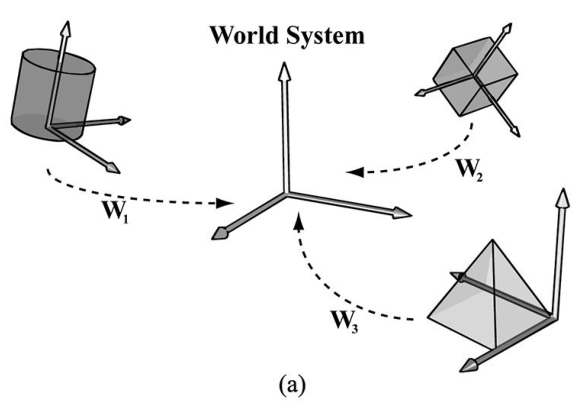
\includegraphics[width=\textwidth]{5-16}
    \centering
    \caption{(a)每个对象的顶点用相对于它们自己的局部坐标系的坐标定义。 另外,我们根据我们想要场景中的对象来定义每个局部坐标系相对于世界空间坐标系的位置和方向。 然后我们执行坐标变换的更改,以使所有坐标相对于世界空间系统。 (b)在世界变换之后,对象的顶点具有相对于同一世界系统的所有坐标。}
    \label{fig:5-16}
\end{figure}

\begin{figure}[t]
    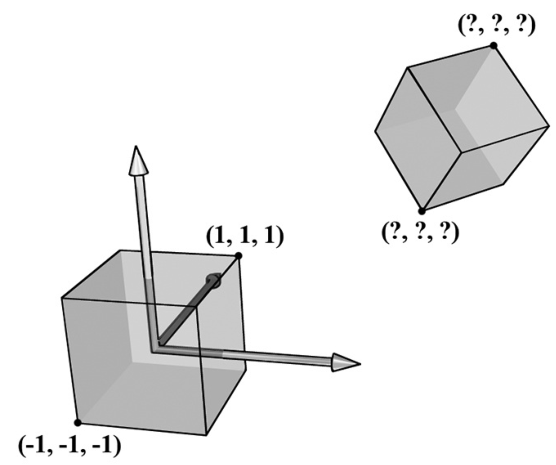
\includegraphics[width=\textwidth]{5-17}
    \centering
    \caption{当立方体在原点居中并与坐标系轴对齐时,可以轻松指定立方体的顶点。 当立方体相对于坐标系处于任意位置和方向时,指定坐标并不容易。 因此,当我们构造一个对象的几何体时,我们通常总是在对象附近选择一个方便的坐标系并与对象对齐,从中构建对象。}
    \label{fig:5-17}
\end{figure}
\begin{flushleft}
相对于自己的局部坐标系定义每个模型有几个优点:\\
\end{flushleft}
\begin{itemize}
  \item 1. 更方便。例如,通常在局部空间中,对象将以原点为中心并相对于一个主轴对称。 另一个例子,如果我们选择一个原点位于立方体并且轴与立方体面正交的局部坐标系,则立方体的顶点更容易指定; 见图\ref{fig:5-17}。
  \item 2. 该对象可以在多个场景中重复使用,在这种情况下,相对于特定场景硬编码对象的坐标是没有意义的。 相反,最好相对于局部坐标系存储其坐标,然后通过坐标矩阵的变化来定义局部坐标系和世界坐标系如何与每个场景相关。
  \item 3. 最后,有时我们在场景中不止一次地绘制相同的对象,但是在不同的位置,方向和比例(例如,树对象可以多次重复使用以构建森林)。 复制每个实例的对象的顶点和索引数据将是浪费的。 相反,我们存储相对于其局部空间的几何(即顶点和索引列表)的单个副本。 然后我们多次绘制对象,但每次都使用不同的世界矩阵来指定实例在世界空间中的位置,方向和比例。 这称为实例化。
\end{itemize}
\begin{flushleft}
如3.4.3节所示,对象的世界矩阵是通过用相对于世界空间的坐标描述其局部空间,并将这些坐标放在矩阵的行中给出的。如果$Q_{w}=(Q_{x},Q_{y},Q_{z},1)$,则$u_{w}=(u_{x},u_{y},u_{z},0)$,$v_{w}=(v_{x},v_{y},v_{z},0)$,并且$w_{w}=(w_{x},w_{y},w_{z},0)$分别描述了具有相对于世界空间的齐次坐标的局部空间的原点,x轴,y轴和z轴,然后我们从3.4.3节中知道坐标矩阵从局部空间到世界空间变化是:\\
\end{flushleft}
\begin{align*}
W=
\begin{bmatrix}
u_{x} & u_{y} & u_{z} & 0\\
v_{x} & v_{y} & v_{z} & 0\\
w_{x} & w_{y} & w_{z} & 0\\
Q_{x} & Q_{y} & Q_{z} & 1
\end{bmatrix}\\
\end{align*}
\begin{flushleft}
我们看到,要构造一个世界矩阵,我们必须直接计算出局部空间原点的坐标和相对于世界空间的轴。 这有时不那么容易或直观。更常见的方法是将 $W$ 定义为变换序列,例如 $W=SRT$,缩放矩阵 $S$ 的乘积,用于将对象缩放到世界中,接着是旋转矩阵 $R$,以定义局部空间相对于的方向。 世界空间,后面是一个平移矩阵 $T$,用于定义相对于世界空间的局部空间的起源。 从3.5节开始,我们知道这个变换序列可以解释为坐标变换的变化,并且 $W=SRT$ 的行向量存储$x$轴,$y$轴,$z$轴和原点的齐次坐标。相对于世界空间的局部空间。
\end{flushleft}

\begin{flushleft}
例子:\\
假设我们有一个相对于某个局部空间定义的单位方形平面,分别具有最小和最大点$(-0.5,0,-0.5)$和$(0.5,0,0.5)$。 找到世界矩阵,使得正方形在世界空间中的长度为$2$,正方形在世界空间的$xz$平面中顺时针旋转$45^{\circ}$,并且正方形位于世界空间的 $(10,0,10)$ 处。 我们按如下方式构造 $S$,$R$,$T$和$W$:\\
\end{flushleft}
\begin{align*}
S=
\begin{bmatrix}
2 & 0 & 0 & 0\\
0 & 1 & 0 & 0\\
0 & 0 & 2 & 0\\
0 & 0 & 0 & 1
\end{bmatrix}
R=
\begin{bmatrix}
\sqrt{2}/2 & 0 & -\sqrt{2}/2 & 0\\
0 & 1 & 0 & 0\\
\sqrt{2}/2 & 0 & \sqrt{2}/2 & 0\\
0 & 0 & 0 & 1
\end{bmatrix}
T=
\begin{bmatrix}
1 & 0 & 0 & 0\\
0 & 1 & 0 & 0\\
0 & 0 & 1 & 0\\
10 & 0 & 10 & 1
\end{bmatrix}\\
W=SRT=
\begin{bmatrix}
\sqrt{2} & 0 & -\sqrt{2} & 0\\
0 & 1 & 0 & 0\\
\sqrt{2} & 0 & \sqrt{2} & 0\\
10 & 0 & 10 & 1
\end{bmatrix}
\end{align*}

\begin{flushleft}
现在从3.5节开始,$W$ 中的行描述了相对于世界空间的局部坐标系; 也就是说,$u_{w}=(\sqrt{2},0,-\sqrt{2},0),v_{w}=(0,1,0,0),w_{w}=(\sqrt{2},0,\sqrt{2},0)$,并且 $Q_{w}=(10,0,10,1)$。 当我们用 $W$ 将局部空间转变为世界空间的坐标时,方形平面也就位于世界空间中的所需位置了(见图\ref{fig:5-18})。
\end{flushleft}

\begin{align*}
[-0.5,0,-0.5,1]W=[10-\sqrt{2},0,0,1]\\
[-0.5,0,+0.5,1]W=[0,0,10+\sqrt{2},1]\\
[+0.5,0,+0.5,1]W=[10+\sqrt{2},0,0,1]\\
[+0.5,0,-0.5,1]W=[0,0,10-\sqrt{2},1]\\
\end{align*}
\begin{flushleft}
这个例子的要点是,我们不是直接计算$Q_{w}$,$u_{w}$,$v_{w}$ 和 $w_{w}$来形成世界矩阵,而是通过合成一系列简单变换来构造世界矩阵。 这通常比直接计算$Q_{w}$,$u_{w}$,$v_{w}$ 和 $w_{w}$容易得多,因为我们只需要问:我们希望物体在世界空间中的大小,我们希望物体在世界空间中的方向, 我们在什么位置想要世界空间中的物体。
\end{flushleft}

\begin{figure}[t]
    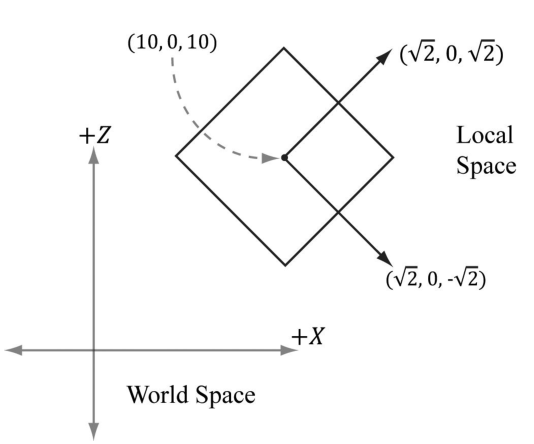
\includegraphics[width=\textwidth]{5-18}
    \centering
    \caption{世界矩阵的行向量描述了具有相对于世界坐标系的坐标的局部坐标系。}
    \label{fig:5-18}
\end{figure}

\begin{flushleft}
考虑世界变换的另一种方法是仅采用局部空间坐标并将它们视为世界空间坐标(这相当于使用单位矩阵作为世界变换)。 因此,如果对象在其局部空间的中心建模,则该对象恰好位于世界空间的中心。 一般来说,世界的中心可能不是我们想要定位所有物体的地方。 所以现在,对于每个对象,只需应用一系列变换来缩放,旋转和定位您想要在世界空间中的对象。 在数学上,这将给出与从局部空间到世界空间的坐标矩阵变化相同的世界变换。
\end{flushleft}

\subsection{视图空间(View Space)}
\begin{flushleft}
为了形成场景的二维图像,我们必须在场景中放置一个虚拟相机。 相机指定了观众可以看到的世界的多大的体积,以及我们需要生成多大的世界体积来生成二维图像。让我们将一个局部坐标系统(称为视图空间,眼图空间或相机空间)附加到相机,如图\ref{fig:5-19}所示; 也就是说,摄像机坐落在正视z轴的原点处,x轴指向摄像机的右侧,y轴指向摄像机的上方。 而不是描述相对于世界空间的场景顶点,基于相机坐标系,渲染管线的后面阶段很方便地描述它们。从世界空间到视图空间的坐标变换称为视图变换,相应的矩阵称为视图矩阵。\\
\begin{figure}[t]
    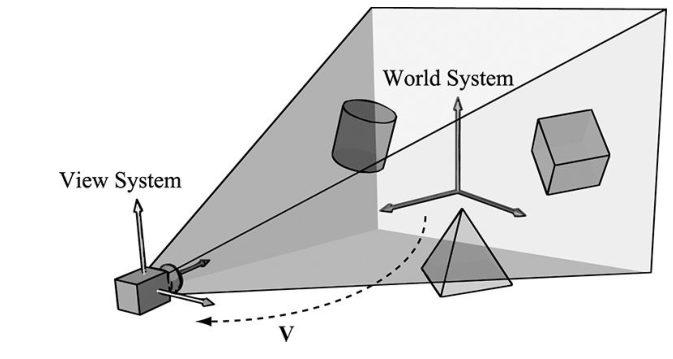
\includegraphics[width=\textwidth]{5-19}
    \centering
    \caption{转换顶点相对于世界空间的坐标,使它们相对于相机空间。}
    \label{fig:5-19}
\end{figure}
如果$Q_{w}=(Q_{x},Q_{y},Q_{z},1)$,$u_{w}=(u_{x},u_{y},u_{z},0)$,$v_{w}=(v_{x},v_{y},v_{z},0)$,$w_{w}=(w_{x},w_{y},w_{z},0)$分别用相对于世界空间的齐次坐标来描述视图空间的原点,x轴,y轴和z轴,然后我们从3.4.3一节知道坐标矩阵从视图空间的变化到世界空间是:
$$W=
\begin{bmatrix}
u_{x} & u_{y} & u_{z} & 0\\
v_{x} & v_{y} & v_{z} & 0\\
w_{x} & w_{y} & w_{z} & 0\\
Q_{x} & Q_{y} & Q_{z} & 1
\end{bmatrix}$$\\
然而,这不是我们想要的转换。我们想要的是倒置转换,即从世界空间转换成视图空间。回忆3.4.3节,倒置转换就是求矩阵的逆。因此$W^{-1}$就是从世界空间到视图空间的转换。\\
世界坐标系统和视图坐标系统仅在位置和方向有区别,所以直观地得到 $W=RT$(也就是说世界矩阵能被分解为一个旋转跟一个平移(translation))\footnote{$R$是\href{https://en.wikipedia.org/wiki/Orthogonal_matrix}{\textcolor{linkColor}{正交矩阵}},所以有 $R^{-1}=R^{T}$}。这让求逆变得简单:
\begin{align*}
V&=W^{-1}=(RT)^{-1}=T^{-1}R^{-1}=T^{-1}R^{T} \\
&=\begin{bmatrix}
1 & 0 & 0 & 0\\
0 & 1 & 0 & 0\\
0 & 0 & 1 & 0\\
-Q_{x} & -Q_{y} & -Q_{z} & 1
\end{bmatrix}
\begin{bmatrix}
u_{x} & v_{x} & w_{x} & 0\\
u_{y} & v_{y} & w_{y} & 0\\
u_{z} & v_{z} & w_{z} & 0\\
0 & 0 & 0 & 0
\end{bmatrix} \\
&=\begin{bmatrix}
u_{x} & v_{x} & w_{x} & 0\\
u_{y} & v_{y} & w_{y} & 0\\
u_{z} & v_{z} & w_{z} & 0\\
\mathbf{-Q\cdot u} & \mathbf{-Q\cdot v} & \mathbf{-Q\cdot w} & 1
\end{bmatrix}
\end{align*}

所以,视图矩阵就是:
\begin{align*}
V=\begin{bmatrix}
u_{x} & v_{x} & w_{x} & 0\\
u_{y} & v_{y} & w_{y} & 0\\
u_{z} & v_{z} & w_{z} & 0\\
\mathbf{-Q\cdot u} & \mathbf{-Q\cdot v} & \mathbf{-Q\cdot w} & 1
\end{bmatrix}
\end{align*}
现在我们用一种直观的方式来构造向量,这些向量用来建立视图矩阵。令\textbf{Q}为摄像机的位置,\textbf{T}为摄像机对准的目标点。然后,令\textbf{j}为世界空间向上方向的单位向量。(本书中,世界坐标系的 xz 构成的平面作为世界地平面,世界 y 轴描述了向上的方向;所以,$j=(0,1,0)$ 就是和世界 y 轴平行的单位向量。然而这只是约定,一些应用可能会选择 xy构成的平面作为地平面,z轴作为向上方向。)参考图片\ref{fig:5-20},摄像机的朝向如下:
$$w=\frac{T-Q}{||T-Q||}$$
该向量描述的是摄像机的z轴,对准\textbf{w}右侧的单位向量:\\
$$u=\frac{j\times w}{||j \times w||}$$
该向量描述的是摄像机的 x 轴。最后,摄像机的y轴单位向量为:\\
$$v=w \times u$$
因为\textbf{w}和\textbf{u}是互相正交的单位向量,$w\times u$也必定是单位向量,没必要正规化。\\
综上所述,给定摄像机的位置,目标点,和世界向上方向,我们就能求得摄像机的本地坐标系统,作为视图矩阵。
\begin{figure}[t]
    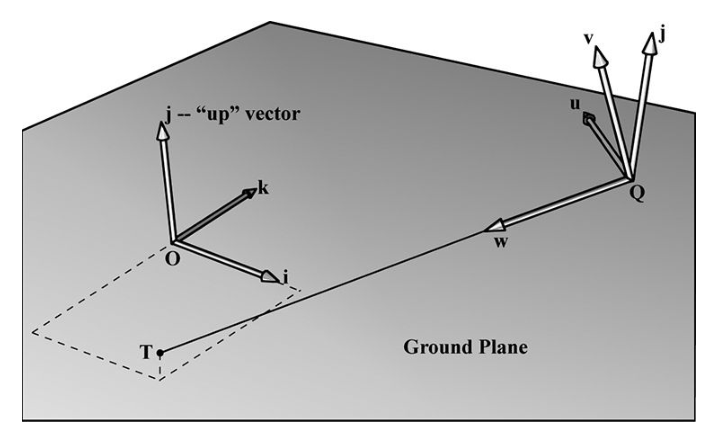
\includegraphics[width=\textwidth]{5-20}
    \centering
    \caption{根据相机位置,目标点和世界“向上”矢量构造相机坐标系。}
    \label{fig:5-20}
\end{figure}

DirectXMath 库提供了计算视图矩阵的方法:
\begin{lstlisting}
// Outputs view matrix V
XMVECTOR XM_CALLCONV XMMatrixLookAtLH(
    FXMVECTOR EyePosition,    // Input camera position Q
    FXMVECTOR FocusPosition,  // Input target point T
    FXMVECTOR UpDirection);   // Input world up direction j
\end{lstlisting}
通常世界y轴就是向上的方向,所以$j=(0,1,0)$ 就是向上的向量。例:假设我们将摄像机放在相对于世界坐标的$(5,3,-10)$处,并且对准世界原点坐标$(0,0,0)$。可以通过下面方式获得视图矩阵:\\
\begin{lstlisting}
XMVECTOR pos    = XMVectorSet(5, 3, -10, 1.0f);
XMVECTOR target = XMVectorZero();
XMVECTOR up     = XMVectorSet(0.0f, 1.0f, 0.0f, 0.0f);
XMMATRIX V      = XMMatrixLookAtLH(pos, target, up);
\end{lstlisting}
\end{flushleft}
\subsection{投影和齐次裁剪空间(Projection and Homogeneous Clip Space)}
\begin{flushleft}
到目前为止我们描述了在世界空间中摄像机的位置和方向,但摄像机还有一个部分需要解决,即摄像机看到的空间体积。体积由视锥来描述(见图\ref{fig:5-21})。
\end{flushleft}
\begin{figure}[t]
    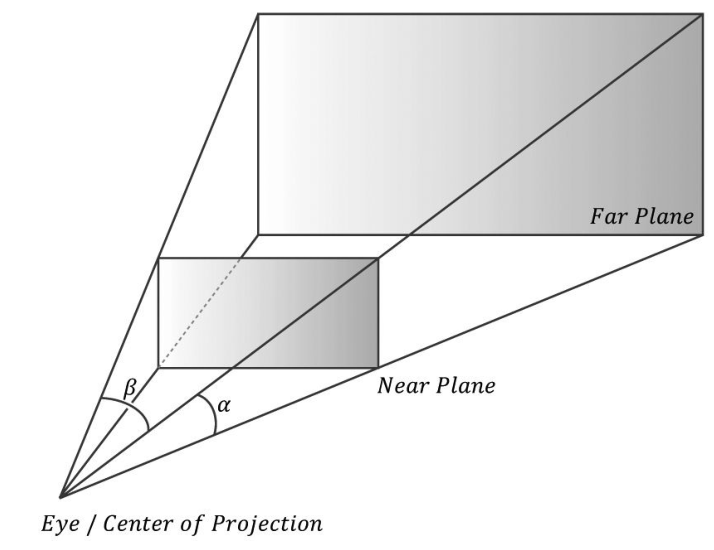
\includegraphics[width=\textwidth]{5-21}
    \centering
    \caption{视锥定义了摄像机“看到”的空间体积}
    \label{fig:5-21}
\end{figure}
\begin{flushleft}
我们接下来的任务是将一个 3D 几何体在视锥中投影到 2D 投影窗口中。投影必须以平行线汇聚到消失点的方式完成,当一个物体的3D深度增加(距离拉远),投影的大小就减小。这就是\href{https://en.wikipedia.org/wiki/Perspective_(graphical)}{\textcolor{linkColor}{透视投影}}(如图\ref{fig:5-22})。我们将一个顶点到视点(眼睛所在的位置,姑且叫视点吧)的连线称为顶点的投影线。然后我们定义透视投影变换就是3D顶点\textbf{v}变换成它的投影线和2D投影面板交叉点\textbf{v'}的过程;我们认为\textbf{v'}就是\textbf{v}的投影。一个3D物体的投影就是组成这个物体的所有顶点的投影。
\end{flushleft}
\begin{figure}[t]
    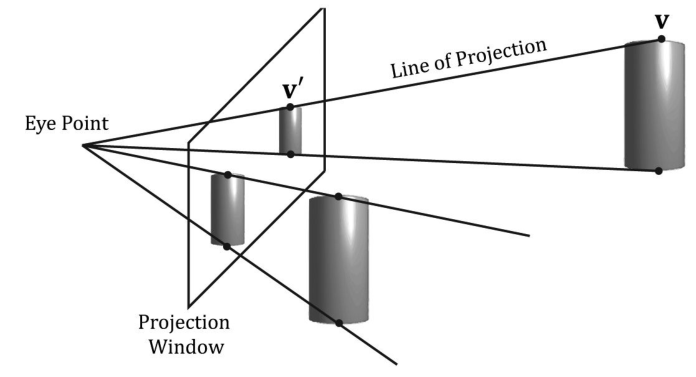
\includegraphics[width=\textwidth]{5-22}
    \centering
    \caption{两个圆柱体大小相同,但深度不同。距离眼睛近的圆柱体比距离远的圆柱体投影大。视锥中的几何体被投影到投影窗口;视锥外的集合体,投影到投影面板上,但在投影窗口外面(投影面板和投影窗口共面)}
    \label{fig:5-22}
\end{figure}

\paragraph{定义一个视锥(Defining a Frustum)}
\begin{flushleft}
我们可以在视图空间中定义一个视锥,其投影中心位于原点处,并沿着正z轴向下看,通过以下四个量:近平面$n$,远平面$f$,垂直视场角$\alpha$ 和纵横比 $r$。请注意,在视图空间中,近平面和远平面平行于$xy$平面; 因此我们只需指定它们沿着z轴的原点距离。 纵横比由 $r=w/h$ 定义,其中$w$是投影窗口的宽度,$h$是投影窗口的高度(视图空间中的单位)。 投影窗口本质上是视图空间中场景的二维图像。 这里的图像最终将映射到后台缓冲区(back buffer); 因此,我们喜欢投影窗口尺寸的比率与后台缓冲区尺寸的比率相同。所以后缓冲区维度的比率通常被指定为长宽比(这是一个比例,所以它没有单位)。例,如果后台缓冲区尺寸是 $800 \times 600$,则 $r=\frac{800}{600} \approx 1.333$。如果投影窗口与后台缓冲区的纵横比不相同,则需要非均匀缩放来将投影窗口映射到后台缓冲区,这将导致失真(例如,投影窗口上的圆圈可能当映射到后台缓冲区时被拉伸成一个椭圆)。\\
我们将水平视角标记为$\beta$,垂直视角标记为$\alpha$,纵横比为$r$。要看看$r$如何帮助我们找到$\beta$,请考虑图\ref{fig:5-23}。 请注意,投影窗口的实际尺寸并不重要,只需要保持纵横比。 因此,我们会选择2的方便高度,因此宽度必须为:\\
$$r=\frac{w}{h}=\frac{w}{2}\Rightarrow w=2r$$
\end{flushleft}
\begin{figure}[t]
    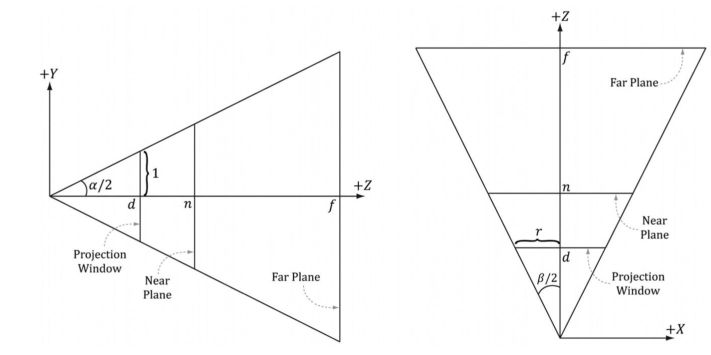
\includegraphics[width=\textwidth]{5-23}
    \centering
    \caption{给定垂直视角$\alpha$和纵横比$r$,得出水平视角$\beta$}
    \label{fig:5-23}
\end{figure}
\begin{flushleft}
为了具有指定的垂直视场$\alpha$,投影窗口必须放置在距离原点的距离$d$处:
$$\tan(\frac{\alpha}{2})=\frac{1}{d}\Rightarrow d=\cot(\frac{\alpha}{2})$$
现在我们已经将投影窗沿$z$轴的距离d固定为当投影窗的高度为2时垂直视场$\alpha$。现在我们可以求解$\beta$。 看一下图\ref{fig:5-23}中的$xz$平面,我们现在看到:
$$\tan(\frac{\beta}{2})=\frac{r}{d}=\frac{r}{\cot(\frac{\alpha}{2})}=r\cdot \tan(\frac{\alpha}{2})$$
因此,考虑到垂直视角α和纵横比r,我们总能得到水平视角β:
$$\beta=2\tan^{-1}(r\cdot\tan(\frac{\alpha}{2}))$$
\end{flushleft}

\paragraph{投影顶点(Projecting Vertices)}
\begin{figure}[t]
    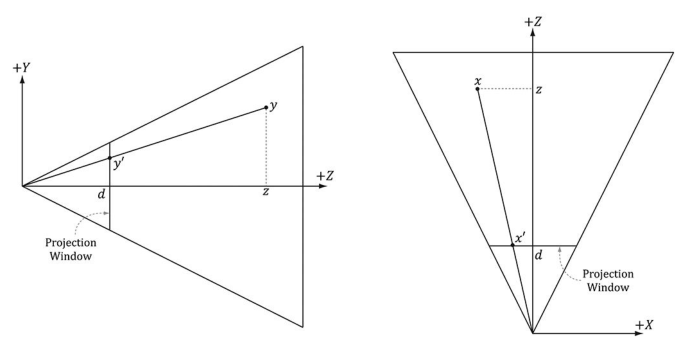
\includegraphics[width=\textwidth]{5-24}
    \centering
    \caption{相似三角}
    \label{fig:5-24}
\end{figure}
\begin{flushleft}
参考图\ref{fig:5-24}。 给定一个点$(x,y,z)$,我们希望在投影平面$z = d$上找到它的投影$(x',y',d)$。 通过分别考虑$x$和$y$坐标并使用相似的三角形,我们发现:
\begin{align*}
\frac{x'}{d}=\frac{x}{z}\Rightarrow x'=\frac{xd}{z}=\frac{x\cot(\alpha/2)}{z}=\frac{x}{z\tan(\alpha/2)}\\
\frac{y'}{d}=\frac{y}{z}\Rightarrow y'=\frac{yd}{z}=\frac{y\cot(\alpha/2)}{z}=\frac{y}{z\tan(\alpha/2)}\\
\end{align*}
显然对于点$(x,y,z)$, $-r\leq x'\leq r,-1\leq y'\leq 1,n\leq z\leq f$
\end{flushleft}

\paragraph{标准化的设备坐标(Normalized Device Coordinate-NDC)}
\begin{flushleft}
上一节中投影点的坐标是在视图空间中计算的。 在视图空间中,投影窗口的高度为2,宽度为$2r$,其中$r$是纵横比。 问题在于,尺寸取决于宽高比。 这意味着我们需要告诉硬件高宽比,因为硬件稍后需要做一些涉及投影窗口尺寸的操作(比如将其映射到后台缓冲区)。 如果我们能够消除这种对长宽比的依赖性会更方便。 解决的办法是将投影的$x$坐标从区间$[-r,r]$缩放到$[-1,1]$像这样:
\begin{align*}
-r\leq x' \leq r \\
-1\leq x'/r \leq 1
\end{align*}

在映射之后,$x$坐标和$y$坐标被称为标准化的设备坐标(NDC)(z坐标还没有被标准化),并且点$(x,y,z)$在视锥内当且仅当:
\begin{align*}
-1\leq x'/r \leq 1 \\
-1\leq y' \leq 1 \\
n \leq z \leq f
\end{align*}

从视图空间到NDC空间的转换可视为单位转换。 我们有一个关系,即一个NDC单位在$x$轴上等于视图空间中的$r$个单位(即 1ndc = \textbf{r} vs)。 所以给定$x$个视图空间单位,我们可以使用这个关系来转换单位:
$$x\mathit{vs}\cdot \frac{1\mathit{ndc}}{r\mathit{vs}}=\frac{x}{r}\mathit{ndc}$$
我们可以修改我们的投影公式,直接在NDC坐标中为我们提供投影的$x$坐标和$y$坐标:
\begin{align*}\tag{eq.5.1}\label{eq.5.1}
x'&=\frac{x}{rz\tan(\alpha/2)}\\
y'&=\frac{y}{z\tan(\alpha/2)}
\end{align*}
请注意,在NDC坐标中,投影窗口的高度为2,宽度为2.因此,现在尺寸是固定的,硬件无需知道纵横比,但我们有责任始终在NDC中提供投影坐标空间(图形硬件假设我们会)。
\end{flushleft}

\paragraph{用矩阵来描述投影公式(Writing the Projection Equations with a Matrix)}
\begin{flushleft}
为了保持一致,我们将用一个矩阵来描述投影变换。不过,公式\ref{eq.5.1}是非线性的,无法用矩阵描述。所以我们要使用一种“技巧”将它分为两部分来实现:一个线性部分和一个非线性部分。非线性部分要除以$z$。我们会在下一节讨论“如何规范化$z$坐标”时讲解这一问题;现在读者只需要知道,我们会因为个除法操作而失去原始的z坐标。所以,我们必须在变换之前保存输入的z坐标;我们可以利用齐次坐标来解决一问题,将输入的$z$坐标复制给输出的$w$坐标。在矩阵乘法中,我们要将元素[2][3]设为1、元素[3][3]设为0(从0开始的索引)。我们的投影矩阵大致如下:
\begin{align*}
P=\begin{bmatrix}
\frac{1}{r\tan(\alpha/2)} & 0 & 0 & 0\\
0 & \frac{1}{\tan(\alpha/2)} & 0 & 0\\
0 & 0 & A & 1\\
0 & 0 & B & 0
\end{bmatrix}
\end{align*}
注意矩阵中的常量$A$和$B$(它们将在下一节讨论);这些常量用于把输入的$z$坐标变换到规范化区间。将一个任意点$(x,y,z,1)$与该矩阵相乘,可以得到:
\begin{align*}\tag{eq.5.2}\label{eq.5.2}
[x,y,z,1]\begin{bmatrix}
\frac{1}{r\tan(\alpha/2)} & 0 & 0 & 0\\
0 & \frac{1}{\tan(\alpha/2)} & 0 & 0\\
0 & 0 & A & 1\\
0 & 0 & B & 0
\end{bmatrix}=\left[ \frac{x}{r\tan(\alpha/2)},\frac{y}{\tan(\alpha/2)},Az+B,z\right]
\end{align*}
在与投影矩阵(线性部分)相乘之后,我们要将每个坐标除以$w = z$(非线性部分),得到最终的变换结果:
\begin{align*}\tag{eq.5.3}\label{eq.5.3}
\left[ \frac{x}{r\tan(\alpha/2)},\frac{y}{\tan(\alpha/2)},Az+B,z\right]
\xrightarrow[]{\text{除以$w$}}
\left[ \frac{x}{rz\tan(\alpha/2)},\frac{y}{z\tan(\alpha/2)},A+\frac{B}{z},1\right]
\end{align*}
顺便提一句,你可能会问:“如何处理除数为0的情况”;对于一问题我们不必担心,因为近平面总是大于0的,其他的点都会被裁剪掉(参见5.9节)。有时,与$w$相除的过程也称为透视除法(perspective divide)或齐次除法(homogeneous divide)。我们可以看到$x$、$y$的投影坐标与公式\ref{eq.5.1}相同。
\end{flushleft}

\paragraph{规范化深度值}
\begin{flushleft}
你可能认为在投影之后可以丢弃原始的3D $z$坐标,因为所有的投影点已经摆放在2D投影窗口上,形成了我们最终看到的2D图像,不会再使用3D $z$坐标了。其实不然,我们仍然需要为深度缓存算法提供3D深度信息。就如同Direct3D希望我们把$x$、$y$投影坐标映射到一个规范化区间一样,Direct3D也希望我们将深度坐标映射到一个规范化区间$[0,1]$中。所以,我们需要创建一个保序函数(order preserving function)$g(x)$把$[n,f]$区间映射到$[0,1]$区间。由于该函数是保序的,所以当$z_{1},z_{2}∈[n,f]$且$z_{1}<z_{2}$时,必有$g(z_{1})<g(z_{2})$。这样,即使深度值已经被变换过了,相对的深度关系还是会被完好无损地保留下来,我们依然可以在规范化区间中得到正确的深度测试结果,这就是我们要为深度缓存算法做的全部工作。
通过缩放和平移可以实现从$[n ,f]$到$[0,1]$的映射。但是,这种方式无法与我们当前的投影方程整合。我们可以从公式\ref{eq.5.3}中看到经过变换的$z$坐标为:
$$g(z)=A+\frac{B}{z}$$
我们现在需要让$A$和$B$满足以下条件:
\begin{itemize}
    \item 条件1:$g(n)=A+\frac{B}{n}$(近平面映射为0)
    \item 条件2:$g(f)=A+\frac{B}{f}$(远平面映射为1)
\end{itemize}
由条件1得到$B$的结果为:$B=-An$。把它代入条件2,得到$A$的结果为:
\begin{align*}
A+\frac{-An}{f}=1\\
\frac{Af-An}{f}=1\\
Af-An=f\\
A=\frac{f}{f-n}
\end{align*}
所以:
\begin{align*}
g(z)=\frac{f}{f-n}-\frac{nf}{(f-n)z}
\end{align*}
从$g(z)$的曲线图(图\ref{fig:5-25})中可以看出,它会限制增长的幅度(保序)而且是非线性的。从图中我们还可以看到,区间中的大部分取值落在近平面附近。因此,大多数深度值被映射到了一个很窄的取值范围内。这会导致深度缓冲区出现精度问题(由于所能表示的数值范围有限,计算机将无法识别变换后的深度值之间的微小差异)。通常的建议是让近平面和远平面尽可能接近,把深度的精度性问题减小到最低程度。
\end{flushleft}
\begin{figure}[b]
    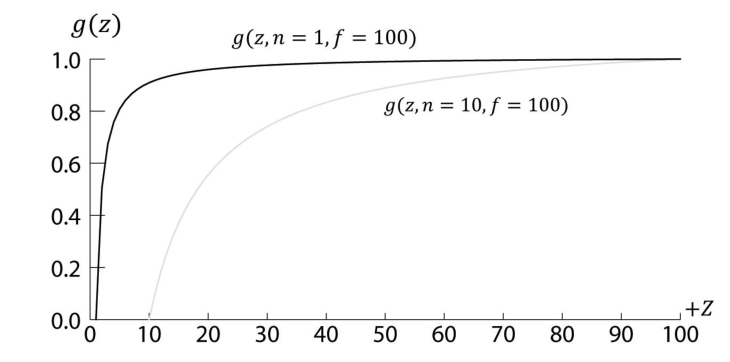
\includegraphics[width=\textwidth]{5-25}
    \centering
    \caption{相对于不同近平面的$g(z)$曲线图}
    \label{fig:5-25}
\end{figure}
\begin{flushleft}
现在我们已经解出了A和B,我们可以确定出完整的透视投影矩阵:
\begin{align*}
P=\begin{bmatrix}
\frac{1}{r\tan(\alpha/2)} & 0 & 0 & 0\\
0 & \frac{1}{\tan(\alpha/2)} & 0 & 0\\
0 & 0 & \frac{f}{f-n} & 1\\
0 & 0 & \frac{-nf}{f-n} & 0
\end{bmatrix}
\end{align*}
在与投影矩阵相乘之后,进行透视除法之前,几何体所处的空间称为齐次裁剪空间(homogeneous clip space)或投影空间(projection space)。在透视除法之后,几何体所处的空间称为规范化设备空间(normalized device coordinates,简称NDC)。
\end{flushleft}

\paragraph{XMMatrixPerspectiveFovLH}
\begin{flushleft}
一个透视投影矩阵能由下面的 DirectX Math 函数生成:
\begin{lstlisting}
// Return the projection matrix
XMMATRIX XM_CALLCONV XMMatrixPerspectiveFovLH(
    float FovAngleY, // vertical field of view angle in radians
    float Aspecct,     // aspect ratio = width / height
    float NearZ,       // distance to near plane
    float FarZ);         // distance to far plane
\end{lstlisting}
下面代码展示了如何使用 XMMatrixPerspectiveFovLH。这里,我们定义垂直视角为$45^{\circ}$,近平面$z=1$,远平面$z=1000$(这些长度都在视图空间)
\begin{lstlisting}
XMMATRIX P= XMMatrixPerspectiveFovLH(0.25f*XM_PI, AspectRatio(),1.0f,1000.0f);
\end{lstlisting}
纵横比匹配窗口的纵横比:
\begin{lstlisting}
float D3DApp::AspectRatio() const
{
  return static_cast<float>(mClientWidth) / mClientHeight;
}
\end{lstlisting}
\end{flushleft}

\section{镶嵌阶段(曲面细分阶段)(The Tessellation Stages)}
\begin{flushleft}
镶嵌(Tessellation)是指通过添加三角形的方式对一个网格的三角形进行细分,这些新添加的三角形可以偏移到一个新的位置,让网格的细节更加丰富。如图\ref{fig:5-26}
\end{flushleft}
\begin{figure}[h]
    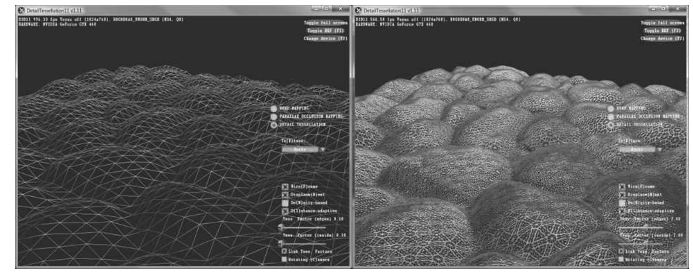
\includegraphics[width=\textwidth]{5-26}
    \centering
    \caption{左图是原网格,右图是镶嵌后的网格}
    \label{fig:5-26}
\end{figure}

\begin{flushleft}
下面是曲面细分的好处:
\begin{itemize}
    \item 我们可以实现细节层次(level-of-detail, LOD),使靠近相机的三角形通过细分产生更多细节,而那些远离相机的三角形则保持不变。通过这种方式,我们只需在需要细节的地方使用更多的三角形就可以了。
    \item 我们可以在内存中保存一个低细节(低细节意味着三角形数量少)的网格,但可以实时地添加额外的三角形,这样可以节省内存。
    \item 我们可以在一个低细节的网格上处理动画和物理效果,而只在渲染时才使用细分过的高细节网格。
\end{itemize}
曲面细分阶段是Direct3D 11中新添加的,这样我们就可以在GPU上对几何体进行细分了。而在Direct3D 11之前,如果你想要实现曲面细分,则必须在CPU上完成,经过细分的几何体还要发送到GPU用于渲染。然而,将新的几何体从CPU内存发送到显存是很慢的,而且还会增加CPU的负担。因此,在Direct3D 11出现之前,曲面细分的方法在实时图形中并不流行。Direct3D 11提供了一个可以完全在硬件上实现的曲面细分API。这样曲面细分就成为了一个非常有吸引力的技术了。曲面细分阶段是可选的(即在需要的时候才使用它)。我们要在第14章才会详细介绍曲面细分。
\end{flushleft}

\section{几何着色阶段(The Geometry Shader Stage)}
\begin{flushleft}
几何着色器阶段(geometry shader stage)是可选的,我们在第12章之前不会用到它,所以这里只做一个简短的概述。几何着色器以完整的图元作为输入数据。例如,当我们绘制三角形列表时,输入到几何着色器的数据是构成三角形的三个点。(注意,这三个点是从顶点着色器传递过来的。)几何着色器的主要优势是它可以创建或销毁几何体。例如,输入图元可以被扩展为一个或多个其他图元,或者几何着色器可以根据某些条件拒绝输出某些图元。这一点与顶点着色器有明显的不同:顶点着色器无法创建顶点,只要输入一个顶点,那么就必须输出一个顶点。几何着色器通常用于将一个点扩展为一个四边形,或者将一条线扩展为一个四边形。\\
~\\
我们可以在图5.11中看到一个“流输出(stream output)”箭头。也就是,几何着色器可以将顶点数据流输出到内存中的一个顶点缓冲区内,这些顶点可以在管线的随后阶段中渲染出来。这是一项高级技术,我们会在后面的章节中对它进行讨论。\\
~\\
NOTICE:顶点位置在离开几何着色器之前,必须被变换到齐次裁剪空间。
\end{flushleft}

\section{裁剪(Clipping)}
\begin{flushleft}
我们必须完全丢弃在平截头体之外的几何体,裁剪与平截头体边界相交的几何体,只留下平截头体内的部分;图 \ref{fig:5-27}以2D形式说明了一概念。
\begin{figure}[h]
    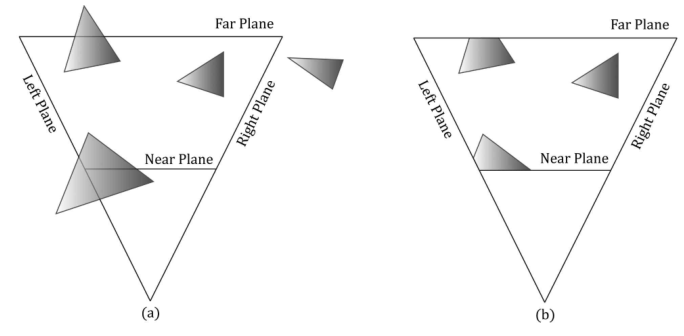
\includegraphics[width=\textwidth]{5-27}
    \centering
    \caption{(a)裁剪之前,(b)裁剪之后}
    \label{fig:5-27}
\end{figure}
我们可以将平截头体视为由6个平面界定的空间范围:顶、底、左、右、近、远平面。要裁剪与平截头体方向相反的多边形,其实就是逐个裁剪与每个平截头体平面方向相反的多边形,当裁剪一个与平面方向相反的多边形时(参见图\ref{fig:5-28}),我们将保留平面正半空间中的部分,而丢弃平面负半空间中的部分。对一个与平面方向相反的凸多边形进行裁剪,得到的结果仍然会是一个凸多边形。由于硬件会自动完成所有的裁剪工作,所以我们不在这里讲解具体的实现细节;有兴趣的读者可以参阅[Sutherland74],了解一下目前流行的Sutherland-Hodgeman裁剪算法。它基本思路是:求出平面与多边形边之间的交点,然后对顶点进行排序,形成新的裁剪后的多边形。\\
\begin{figure}[h]
    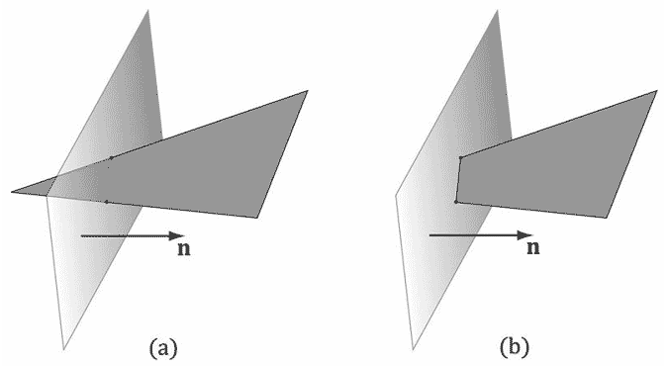
\includegraphics[width=\textwidth]{5-28}
    \centering
    \caption{(a)裁剪一个与平面方向相反的三角形,(b)裁剪后的三角形。注意,裁剪后的三角形已经不再是一个三角形了,它是一个四边形。所以,硬件必须将这个四边形重新划分为三角形,对于凸多边形来说这是一个非常简单的处理过程。}
    \label{fig:5-28}
\end{figure}
\begin{figure}[h]
    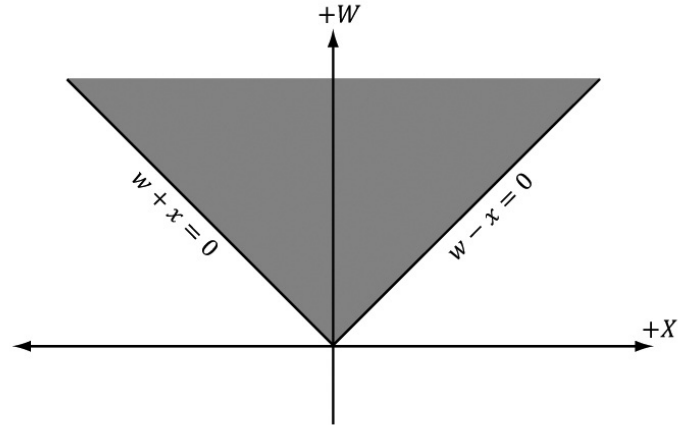
\includegraphics[width=\textwidth]{5-29}
    \centering
    \caption{齐次裁剪空间中$xw$平面上的截头体边界}
    \label{fig:5-29}
\end{figure}
[Blinn78]描述了如何在4D齐次空间中实现裁剪算法(图\ref{fig:5-29})。在透视除法之后,平截头体内的点$ (\frac{x}{w},\frac{y}{w},\frac{z}{w},1) $将位于规范化设备空间,它的边界如下:
\begin{align*}
-1\leq x/w \leq 1\\
-1\leq y/w \leq 1\\
0 \leq z/w \leq 1
\end{align*}
那么在透视除法之前,平截头体内的4D点(x , y , z , w)在齐次裁剪空间中的边界为:
\begin{align*}
-w\leq x \leq w\\
-w\leq y \leq w\\
0 \leq z \leq w
\end{align*}
也就是,顶点被限定在以下4D平面构成的空间范围内:
\begin{align*}
\mathit{Left:}&w=-x\\
\mathit{Right:}&w=x\\
\mathit{Bottom:}&w=-y\\
\mathit{Top:}&w=y\\
\mathit{Near:}&z=0\\
\mathit{Far:}&z=w
\end{align*}
只要我们知道齐次剪裁空间中的平截头体平面方程,我们就能使用任何一种裁剪算法(比如Sutherland-Hodgeman)。注意,由线段/平面相交测试的数学推论可知,这个测试在$\mathbf{R}^{4}$也能使用,所以我们可以在齐次裁剪空间中进行4D点和4D平面的相交测试。
\end{flushleft}

\section{光栅化阶段(The Rasterization Stage)}
\begin{flushleft}
光栅化(rasterization)阶段的主要任务是为投影后的3D三角形计算像素颜色。
\end{flushleft}
\subsection{视口变换(Viewport Transform)}
\begin{flushleft}
在裁剪之后,硬件会自动执行透视除法,将顶点从齐次裁剪空间变换到规范化设备空间(NDC)。一旦顶点进入NDC空间,构成2D图像的2D x、y坐标就会被变换到后台缓冲区中的一个称为视口的矩形区域内(回顾4.2.8节)。在该变换之后,$x$、$y$坐标将以像素为单位。通常,视口变换不修改$z$坐标,因为z坐标还要由深度缓存使用,但是我们可以通过 D3D12\_VIEWPORT 结构体的 MinDepth 和 MaxDepth 值修改z坐标的取值范围。MinDepth 和 MaxDepth 的值必须在0和1之间。
\end{flushleft}
\subsection{背面剔除(Backface Culling)}
\begin{flushleft}
一个三角形有两个面。我们使用如下约定来区分这两个面。假设三角形的顶点按照$v_{0}$、$v_{1}$、$v_{2}$的顺序排列,我们这样来计算三角形的法线$n$:
\begin{align*}
e_{0}&=v_{1}-v_{0}\\
e_{1}&=v_{2}-v_{1}\\
n&=\frac{e_{0}\times e_{1}}{||e_{0}\times e_{1}||}
\end{align*}
带有法线向量的面为正面,而另一个面为背面。图\ref{fig:5-30}说明了这一概念。
\begin{figure}[h]
    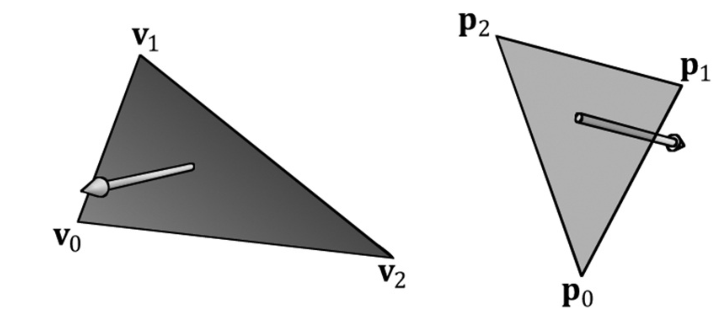
\includegraphics[width=\textwidth]{5-30}
    \centering
    \caption{左边的三角形正对我们的观察点,而右边的三角形背对我们的观察点。}
    \label{fig:5-30}
\end{figure}
当观察者看到三角形的正面时,我们说三角形是朝前的;当观察者看到三角形的背面时, 我们说三角形是朝后的。如图\ref{fig:5-30}所示,左边的三角形是朝前的,而右边的三角形是朝后的。而且,按照我们的观察角度,左边的三角形会按顺时针方向环绕,而右边的三角形会按逆时针方向环绕。这不是巧合:因为按照我们选择的约定(即,我们计算三角形法线的方式),按顺时针方向环绕的三角形(相对于观察者)是朝前的,而按逆时针方向环绕的三角形(相对于观察者)是朝后的。\\
~\\
现在,3D空间中的大部分物体都是封闭实心物体。当我们按照这一方式将每个三角形的法线指向物体外侧时,摄像机就不会看到实心物体朝后的三角形,因为朝前的三角形挡住了朝后的三角形;图\ref{fig:5-31}和图\ref{fig:5-32}分别以2D和3D形式说明了一概念。由于朝前的三角形挡住了朝后的三角形,所以绘制它们是毫无意义的。背面消隐(backface culling)是指让管线放弃对朝后的三角形的处理。这可以将所要处理的三角形的数量降低到原数量的一半。
\end{flushleft}
\begin{figure}[h]
    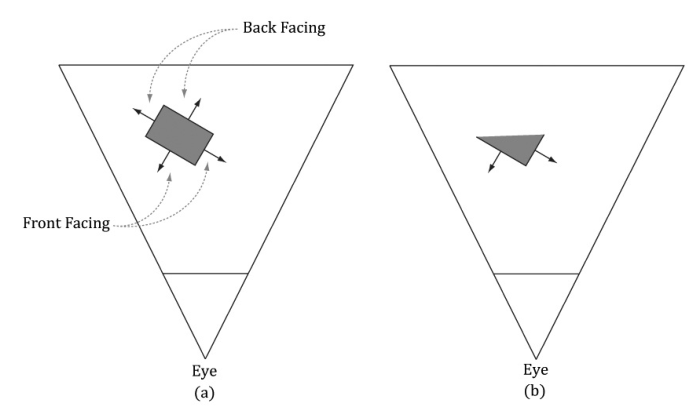
\includegraphics[width=\textwidth]{5-31}
    \centering
    \caption{(a)一个带有朝前和朝后三角形的实心物体。(b)在剔除了朝后的三角形之后的场景。注意,背面消隐不会影响最终的图像,因为朝后的三角形会被朝前的三角形阻挡。}
    \label{fig:5-31}
\end{figure}
\begin{figure}[h]
    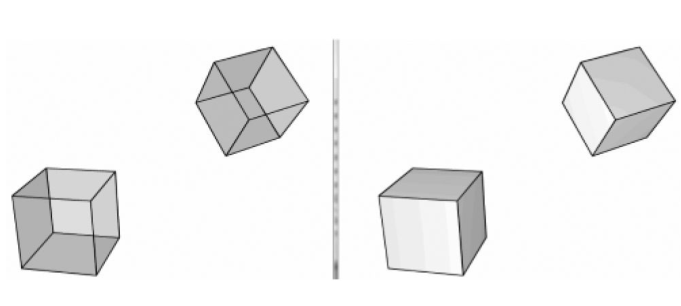
\includegraphics[width=\textwidth]{5-32}
    \centering
    \caption{(左图)当以透明方式绘制立方体时,我们可以看到所有的6个面。(右图)当以实心方式绘制立方体时,我们无法看到朝后的3个面,因为朝前的3个面挡住了它们——所以朝后的三角形可以被直接丢弃,不再接受后续处理,没人能看到些朝后的三角形。}
    \label{fig:5-32}
\end{figure}
\begin{flushleft}
默认情况下,Direct3D将(相对于观察者)顺时针方向环绕的三角形视为朝前的三角形,将(相对于观察者)逆时针方向环绕的三角形视为朝后的三角形。不过,这一约定可以通过修改Direct3D渲染状态颠倒过来。
\end{flushleft}

\subsection{顶点属性插值(Vertex Attribute Interpolation)}
\begin{flushleft}
如前所述,我们通过指定三角形的3个顶点来定义一个三角形。除位置外,顶点还可以包含其他属性,比如颜色、法线向量和纹理坐标。在视口变换之后,这些属性必须为三角形表面上的每个像素进行插值。顶点深度值也必须进行插值,以使每个像素都有一个可用于深度缓存算法的深度值。对屏幕空间中的顶点属性进行插值,其实就是对3D空间中的三角形表面进行线性插值(如图\ref{fig:5-33}所示);这一工作需要借助所谓的透视矫正插值(perspective
correct interpolation)来实现。本质上,三角形表面内部的像素颜色都是通过顶点插值得到的。
\end{flushleft}
\begin{figure}[h]
    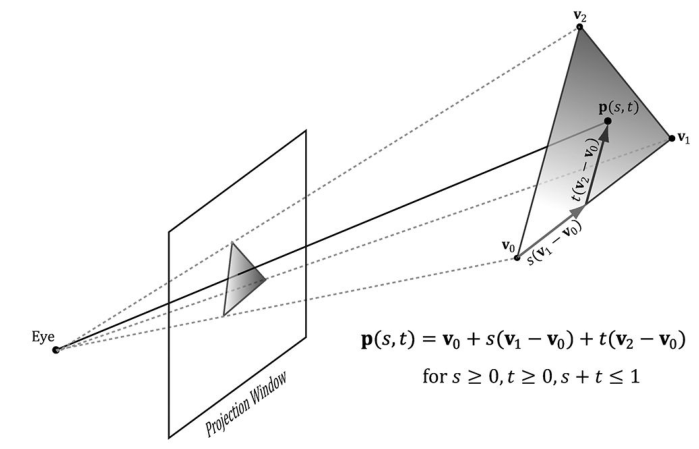
\includegraphics[width=\textwidth]{5-33}
    \centering
    \caption{通过对三角形顶点之间的属性值进行线性插值,可以得到三角形表面上的任一属性值p(s,t)。}
    \label{fig:5-33}
\end{figure}
\begin{flushleft}
我们不必关心透视精确插值的数学细节,因为硬件会自动完成这一工作;不过,有兴趣的读者可以在[Eberly01]中查阅相关的数学推导过程。图5.34介绍了一点基本思路:
\end{flushleft}
\begin{figure}[h]
    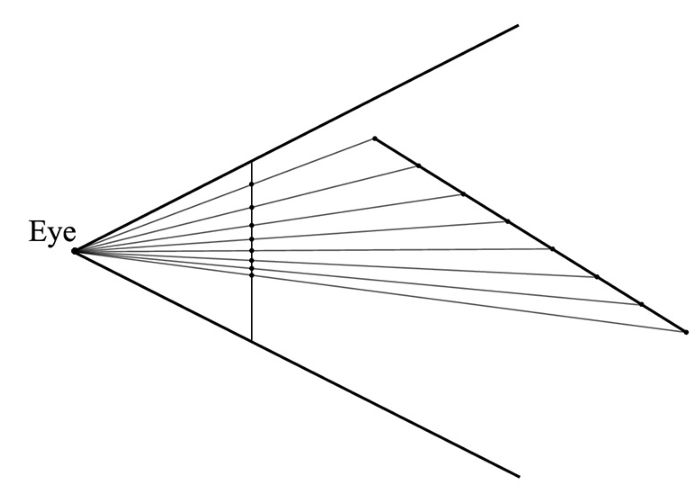
\includegraphics[width=\textwidth]{5-34}
    \centering
    \caption{一条3D线被投影到投影窗口上(在屏幕空间中投影是一条2D线)。我们看到,在3D线上取等距离的点,在2D屏幕空间上的投影点却不是等距离的。所以,我们在3D空间中执行线性插值,在屏幕空间需要执行非线性插值。}
    \label{fig:5-34}
\end{figure}

\section{像素着色器阶段(The Pixel Shader Stage)}
\begin{flushleft}
像素着色器(Pixel shader)是由我们编写的在GPU上执行的程序。像素着色器会处理每个像素片段(pixel fragment),它的输入是插值后的顶点属性,由此计算出一个颜色。像素着色器可以非常简单地输出一个颜色,也可以很复杂,例如实现逐像素光照、反射和阴影等效果。
\end{flushleft}
\section{输出合并阶段(The Output Merger Stage)}
\begin{flushleft}
当像素片段由像素着色器生成之后,它们会被传送到渲染管线的输出合并(output
merger,简称OM)阶段。在该阶段中,某些像素片段会被丢弃(例如,未能通过深度测试或模板测试)。未丢弃的像素片段会被写入后台缓冲区。混合(blending)工作是在该阶段中完成的,一个像素可以与后台缓冲区中的当前像素进行混合,并以混合后的值作为该像素的最终颜色。某些特殊效果,比如透明度,就是通过混合来实现的;我们会在第10章专门讲解混合。
\end{flushleft}
\chapter{在Direct3D中绘制(Drawing in Direct3D)}
\begin{flushleft}
在前一章中,我们主要关注渲染管线的概念和数学方面。 本章反过来关注配置渲染管道,定义顶点和像素着色器以及将几何图形提交到渲染管道进行绘制所需的Direct3D API接口和方法。 到本章结束时,您将能够绘制出具有纯色的3D框或线框模式。\\
~\\
{\large Objectives:}
\begin{itemize}
    \item 发现用于定义,存储和绘制几何数据的Direct3D接口方法。
    \item 学习如何写一个基本顶点和像素着色器
    \item 了解如何用管线状态对象配置渲染管线
    \item 理解如何创建和绑定缓冲数据常量到管线中,并且熟悉根签名
\end{itemize}
\end{flushleft}
\section{顶点和顶点布局(Vertices and Input Layouts)}
\begin{flushleft}
5.5.1节已经讲过,在Direct3D中,顶点由空间位置和各种附加属性组成,Direct3D可以让我们灵活地建立属于我们自己的顶点格式;换句话说,它允许我们定义顶点的分量。要创建一个自定义的顶点格式,我们必须先创建一个包含顶点数据的结构体。例如,下面是两种不同类型的顶点格式;一个由位置和颜色组成,另一个由位置、法线和纹理坐标组成。
\end{flushleft}
\begin{lstlisting}
struct Vertex1
{
    XMFLOAT3 Pos;
    XMFLOAT4 Color;
}
struct Vertex2
{
    XMFLOAT3 Pos;
    XMFLOAT3 Normal;
    XMFLOAT2 Tex0;
    XMFLOAT2 Tex1;
}
\end{lstlisting}
\begin{flushleft}
我们定义好顶点构造体后,需要对该定点构造体进行描述然后提供给 Direct3D,让它知道如何去处理每个分量。此描述以D3D12\_INPUT\_LAYOUT\_DESC结构表示的输入布局描述(input layout description)的形式提供给Direct3D:
\begin{lstlisting}
typedef struct D3D12_INPUT_LAYOUT_DESC
{
    const D3D12_INPUT_ELEMENT_DESC *pInputElementDescs;
    UINT NumElements;
} D3D12_INPUT_LAYOUT_DESC;
\end{lstlisting}
一个输入布局描述就是一个简单的 D3D12\_INPUT\_ELEMENT\_DESC 元素数组和元素的数量。\\
~\\
D3D12\_INPUT\_ELEMENT\_DESC数组中的每个元素描述了对应的顶点结构体的分量。如果顶点构造体有两个分量,则对应的 D3D12\_INPUT\_ELEMENT\_DESC数组就有2个元素。D3D12\_INPUT\_ELEMENT\_DESC 定义如下:
\begin{lstlisting}
typedef struct D3D12_INPUT_ELEMENT_DESC
{
    LPCSTR SemanticName;
    UINT SemanticIndex;
    DXGI_FORMAT Format;
    UINT InputSlot;
    UINT AlignedByteOffset;
    D3D12_INPUT_CLASSIFICATION InputSlotClass;
    UINT InstanceDataStepRate;
} D3D12_INPUT_ELEMENT_DESC;
\end{lstlisting}
1. SemanticName: 一个与元素相关的字符串。它可以是任何有效的语义名。语义(semantic)用于将顶点结构体中的元素映射为顶点着色器参数(参见图\ref{fig:6-1})。\\
\begin{figure}[h]
    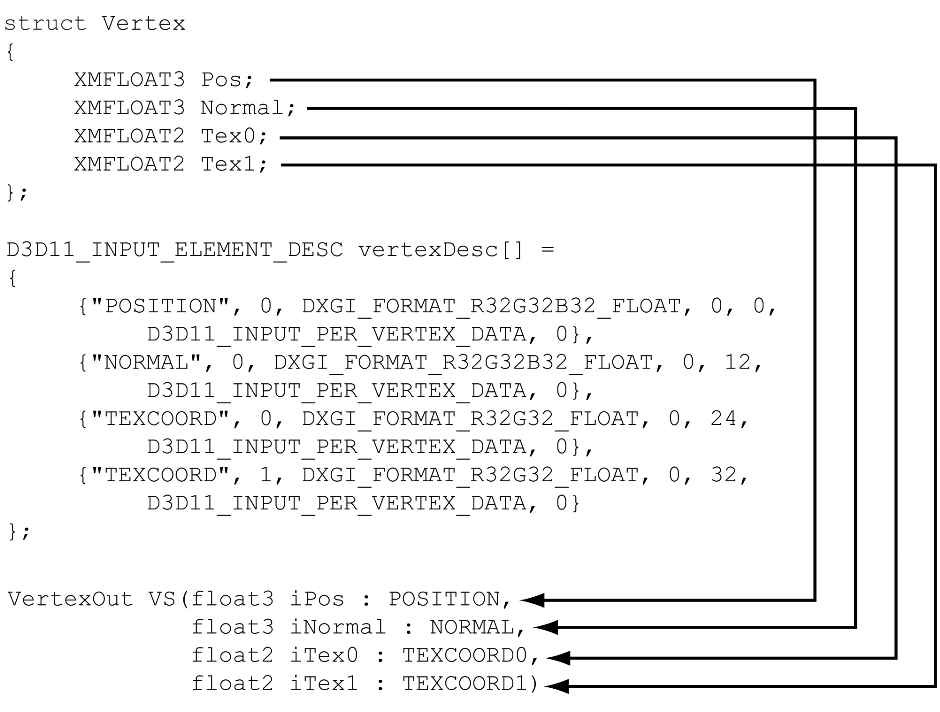
\includegraphics[width=\textwidth]{6-1}
    \centering
    \caption{顶点结构体中的每个元素分别由D3D11\_INPUT\_ELEMENT\_DESC数组中的对应元素描述。语义名和语义索引提供了一种将顶点元素映射为顶点着色器参数的方法。}
    \label{fig:6-1}
\end{figure}
2. SemanticIndex:附加在语义上的索引值。图\ref{fig:6-1}说明了使用该索引的原因;举例来说,当顶点结构体包含多组纹理坐标时,我们不是添加一个新的语义名,而是在语义名的后面加上一个索引值。在着色器代码中没有指定索引的语义默认索引为0,例如,在图\ref{fig:6-1}中的POSITION相当于POSITION0。\\
3. Format:一个用于指定元素格式的DXGI\_FORMAT枚举类型成员;下面是一些常用的格式:
\begin{lstlisting}
DXGI_FORMAT_R32_FLOAT          // 1D 32-bit float scalar
DXGI_FORMAT_R32G32_FLOAT       // 2D 32-bit float vector
DXGI_FORMAT_R32G32B32_FLOAT    // 3D 32-bit float vector
DXGI_FORMAT_R32G32B32A32_FLOAT // 4D 32-bit float vector
DXGI_FORMAT_R8_UINT            // 1D 8-bit unsigned integer scalar
DXGI_FORMAT_R16G16_SINT        // 2D 16-bit signed integer vector
DXGI_FORMAT_R32G32B32_UINT     // 3D 32-bit unsigned integer vector
DXGI_FORMAT_R8G8B8A8_SINT      // 4D 8-bit signed integer vector
DXGI_FORMAT_R8G8B8A8_UINT      // 4D 8-bit unsigned integer vector
\end{lstlisting}
4. InputSlot:指定当前元素来自于哪个输入槽(input slot)。Direct3D支持16个输入槽(索引依次为 0到15),通过这些输入槽我们可以向Direct3D传入顶点数据。例如,当一个顶点由位置元素和颜色元素组成时,我们既可以使用一个输入槽传送两种元素,也可以将两种元素分开,使用第一个输入槽传送顶点元素,使用第二个输入槽传送颜色元素。Direct3D可以将来自于不同输入槽的元素重新组合为顶点。在本书中,我们只使用一个输入槽,但是在本章结尾的练习2中我们会引导读者做一个使用两个输入槽的练习。\\
5. AlignedByteOffset:对于单个输入槽来说,该参数表示从顶点结构体的起始位置到顶点元素的起始位置之间的字节偏移量。例如在下面的顶点结构体中,元素Pos的字节偏移量为0,因为它的起始位置与顶点结构体的起始位置相同;元素Normal的字节偏移量为12,因为必须跳过由Pos占用的字节才能到达Normal的起始位置;元素Tex0的字节偏移量为24,因为必须跳过由Pos和Normal占用的字节才能到达Tex0的起始位置;元素Tex1的字节偏移量为32,因为必须跳过由Pos,Normal和Tex0占用的字节才能到达Tex1的起始位置。\\
\begin{lstlisting}
struct Vertex2
{
    XMFLOAT3 Pos;     // 0-byte offset
    XMFLOAT3 Normal;  // 12-byte offset
    XMFLOAT2 Tex0;    // 24-byte offset
    XMFLOAT2 Tex1;    // 32-byte offset
}
\end{lstlisting}
6. InputSlotClass:目前指定为D3D12\_INPUT\_PER\_VERTEX\_DATA;其他选项用于高级实例技术。\\
7. InstanceDataStepRate:目前指定为0;其他值只用于高级实例技术。\\
~\\
对于前面的两个示例顶点结构体Vertex1和Vertex2来说,对应的输入布局描述为:
\begin{lstlisting}
D3D12_INPUT_ELEMENT_DESC desc1[] = 
{
    {"POSITION", 0, DXGI_FORMAT_R32G32B32_FLOAT, 0, 0, 
                 D3D12_INPUT_PRE_VERTEX_DATA, 0},
    {"COLOR",    0, DXGI_FORMAT_R32G32B32A32_FLOAT, 0, 12, 
                 D3D12_INPUT_PRE_VERTEX_DATA, 0}
};
D3D12_INPUT_ELEMENT_DESC desc2[] =
{
    {"POSITION", 0, DXGI_FORMAT_R32G32B32_FLOAT, 0, 0,  
                 D3D12_INPUT_PRE_VERTEX_DATA, 0},
    {"NORMAL",   0, DXGI_FORMAT_R32G32B32_FLOAT, 0, 12, 
                 D3D12_INPUT_PRE_VERTEX_DATA, 0},
    {"TEXCOORD", 0, DXGI_FORMAT_R32G32_FLOAT, 0, 24, 
                 D3D12_INPUT_PRE_VERTEX_DATA, 0},
    {"TEXCOORD", 1, DXGI_FORMAT_R32G32_FLOAT, 0, 32, 
                 D3D12_INPUT_PRE_VERTEX_DATA, 0}
};
\end{lstlisting}
\end{flushleft}
\section{顶点缓冲(Vertex Buffers)}
\begin{flushleft}
为了让GPU访问顶点数组,我们必须把它放置在一个称为缓冲(buffer)的GPU资源容器中, 我们称存储顶点的缓冲区叫顶点缓冲区。 缓冲区比纹理资源简单; 它们不是多维的,并且没有mipmap,过滤器或多采样支持。 无论何时我们需要为GPU提供一系列数据元素(如顶点),我们都会使用缓冲区。\\
~\\
就像4.3.8节一样,我们通过填充一个 D3D12\_RESOURCE\_DESC结构体来创建一个 ID3D12Resource 对象,并将其作为缓冲区资源。然后调用 ID3D12Device::CreateCommitedResource 方法。D3D12\_RESOURCE\_DESC 成员详情见 4.3.8 节。Direct3D 12 提供一个 C++ 包装类 CD3DX12\_RESOURCE\_DESC,它是 D3D12\_RESOURCE\_DESC 的衍生类,提供了方便的构造函数和方法。特别是,它提供了以下方法来简化描述缓冲区的D3D12\_RESOURCE\_DESC的构造:
\begin{lstlisting}
static inline CD3DX12_RESOURCE_DESC Buffer(
    UINT64 width, 
    D3D12_RESOURCE_FLAGS flags = D3D12_RESOURCE_FLAG_NONE,
    UINT64 alignment = 0)
{
    return CD3DX12_RESOURCE_DESC(D3D12_RESOURCE_DIMENSION_BUFFER, 
            alignment, width, 1, 1, 1, 
            DXGI_FORMAT_UNKNOWN, 1, 0,
            D3D12_TEXTURE_LAYOUT_ROW_MAJOR, flags);
}
\end{lstlisting}
对于一个缓冲区,width 相当于缓冲区的字节数。例,如果一个缓冲区存储64个浮点型(float),则 width 就是 64*sizeof(float)。\\
~\\
NOTICE: CD3DX12\_RESOURCE\_DESC类还提供了其他针对纹理资源和查询资源的方法:\\
\begin{itemize}
    \item 1. CD3DX12\_RESOURCE\_DESC::Tex1D
    \item 2. CD3DX12\_RESOURCE\_DESC::Tex2D
    \item 3. CD3DX12\_RESOURCE\_DESC::Tex3D
\end{itemize}
~\\
NOTICE:回忆第4章深度/模板缓冲区(depth/stencil buffer),这一阶段用ID3D12Resource 来表现 2D 纹理。所有在 Direct3D 12 的资源都用 ID3D12Resource 接口来表示。着和 Direct3D 11 中使用不同的接口表示不同的资源相反,像 ID3D11Buffer,ID3D11Texture2D。资源类型由 D3D12\_RESOURCE\_DESC::D3D12\_RESOURCE\_DIMENSION 属性指定。例:缓冲区有 D3D12\_RESOURCE\_DIMENSION\_BUFFER 和 2D 纹理 D3D12\_RESOURCE\_DIMENSION\_TEXTURE2D。\\
~\\
对于常量几何(不以每帧为基础改变的几何图形),我们将顶点缓冲区(vertex buffer)放入默认堆(D3D12\_HEAP\_TYPE\_DEFAULT)中,以提升性能。通常,一个游戏中大多数几何图形都是常量集合,像树、建筑、地形、人物等。顶点缓冲区初始化之后,只有GPU需要从顶点缓冲区中读取并画几何图形,所以默认堆就变得有意义了。然而,如果CPU不能将顶点缓冲区写入到默认堆中,我们如何才能初始化顶点缓冲区呢?\\
~\\
另外要新建实际的缓冲区资源,我们需要用D3D12\_HEAP\_TYPE\_UPLOAD新建一个中间上传缓冲资源。回忆4.3.8节,当我们需要从CPU到GPU复制数据时,我们将一个资源提交到上传队中。在创建上传缓冲区之后,从系统内存中复制顶点数据到上传缓冲区,然后从上传缓冲区复制顶点数据到实际的顶点缓冲区中。\\
~\\
因为一个中间上传缓冲区需要初始化数据后的默认缓冲区(D3D12\_HEAP\_TYPE\_DEFAULT),所以为了代码重用性 d3dUtil.h/cpp 中建立了下面工具方法:
\begin{lstlisting}
Microsoft::WRL::ComPtr<ID3D12Resource> d3dUtil::CreateDefaultBuffer(
    ID3D12Device* device,
    ID3D12GraphicsCommandList* cmdList,
    const void* initData,
    UINT64 byteSize,
    Microsoft::WRL::ComPtr<ID3D12Resource>& uploadBuffer)
{
ComPtr<ID3D12Resource> defaultBuffer;

    // Create the actual default buffer resource.
    ThrowIfFailed(device->CreateCommittedResource(
        &CD3DX12_HEAP_PROPERTIES(D3D12_HEAP_TYPE_DEFAULT),
        D3D12_HEAP_FLAG_NONE,
        &CD3DX12_RESOURCE_DESC::Buffer(byteSize),
        D3D12_RESOURCE_STATE_COMMON,
        nullptr,
        IID_PPV_ARGS(defaultBuffer.GetAddressOf())));

    // In order to copy CPU memory data into our default buffer, 
    // we need to create an intermediate upload heap. 
    ThrowIfFailed(device->CreateCommittedResource(
        &CD3DX12_HEAP_PROPERTIES(D3D12_HEAP_TYPE_UPLOAD),
        D3D12_HEAP_FLAG_NONE,
        &CD3DX12_RESOURCE_DESC::Buffer(byteSize),
        D3D12_RESOURCE_STATE_GENERIC_READ,
        nullptr,
        IID_PPV_ARGS(uploadBuffer.GetAddressOf())));

    // Describe the data we want to copy into the default buffer.
    D3D12_SUBRESOURCE_DATA subResourceData = {};
    subResourceData.pData = initData;
    subResourceData.RowPitch = byteSize;
    subResourceData.SlicePitch = subResourceData.RowPitch;

    // Schedule to copy the data to the default buffer resource.  
    // At a high level, the helper function UpdateSubresources
    // will copy the CPU memory into the intermediate upload heap.  
    // Then, using ID3D12CommandList::CopySubresourceRegion,
    // the intermediate upload heap data will be copied to mBuffer.
    cmdList->ResourceBarrier(1, 
            &CD3DX12_RESOURCE_BARRIER::Transition(defaultBuffer.Get(), 
                D3D12_RESOURCE_STATE_COMMON, 
                D3D12_RESOURCE_STATE_COPY_DEST));

    UpdateSubresources<1>(cmdList, 
                          defaultBuffer.Get(), 
                          uploadBuffer.Get(),
                          0, 0, 1, 
                          &subResourceData);

    cmdList->ResourceBarrier(1, 
            &CD3DX12_RESOURCE_BARRIER::Transition(defaultBuffer.Get(),
                D3D12_RESOURCE_STATE_COPY_DEST, 
                D3D12_RESOURCE_STATE_GENERIC_READ));

    // Note: uploadBuffer has to be kept alive 
    // after the above function calls because
    // the command list has not been executed 
    // yet that performs the actual copy.
    // The caller can Release the uploadBuffer 
    // after it knows the copy has been executed.
    return defaultBuffer;
}
\end{lstlisting}
D3D12\_SUBRESOURCE\_DATA 结构体定义如下:\\
\begin{lstlisting}
typedef struct D3D12_SUBRESOURCE_DATA
{
    const void *pData;
    LONG_PTR RowPitch;
    LONG_PTR SlicePitch;
} D3D12_SUBRESOURCE_DATA;
\end{lstlisting}
1. pData: 指向系统内存数组的指针,该系统内存数组包含了初始化缓冲区所需要的数据。如果缓冲区能保存 n 个顶点,则系统内存数组必须包含至少 n 个顶点的空间,以此来初始化整个缓冲区。\\
2. RowPitch:对于缓冲区,数据复制的字节大小。\\
3. SlicePitch:对于缓冲区,数据复制的字节大小。\\
~\\
下面代码展示了如何该类如何用于创建一个8顶点立方体的默认缓冲区,并且各个定点颜色不同:\\
\begin{lstlisting}
Vertex vertices[] = 
{
    {XMFLOAT3(-1.0f, -1.0f, -1.0f), XMFLOAT4(Colors::White)},
    {XMFLOAT3(-1.0f, +1.0f, -1.0f), XMFLOAT4(Colors::Black)},
    {XMFLOAT3(+1.0f, +1.0f, -1.0f), XMFLOAT4(Colors::Red)},
    {XMFLOAT3(+1.0f, -1.0f, -1.0f), XMFLOAT4(Colors::Green)},
    {XMFLOAT3(-1.0f, -1.0f, +1.0f), XMFLOAT4(Colors::Blue)},
    {XMFLOAT3(-1.0f, +1.0f, +1.0f), XMFLOAT4(Colors::Yellow)},
    {XMFLOAT3(+1.0f, +1.0f, +1.0f), XMFLOAT4(Colors::Cyan)},
    {XMFLOAT3(+1.0f, -1.0f, +1.0f), XMFLOAT4(Colors::Magenta)}
};
const UINT64 vbByteSize = 8 * sizeof(Vertex);
ComPtr<ID3D12Resource> VertexBufferGPU = nullptr;
ComPtr<ID3D12Resource> VertexBufferUploader = nullptr;
VertexBufferGPU = d3dUtil::CreateDefaultBuffer(
    md3dDevice.Get(),
    mCommandList.Get(),
    vertices, vbByteSize,
    VertexBufferUploader);
\end{lstlisting}
Vertex 类型定义如下:\\
\begin{lstlisting}
struct Vertex
{
    XMFLOAT3 Pos;
    XMFLOAT4 Color;
}
\end{lstlisting}
为了将顶点缓冲区绑定到管道,我们需要为顶点缓冲区资源创建一个顶点缓冲区视图(vertex buffer view)。不像一个RTV(render target view),我们不需要一个针对顶点缓冲区视图的描述堆(descriptor heap)。一个顶点缓冲区视图由 D3D12\_VERTEX\_BUFFER\_VIEW\_DESC 结构体表示:\\
\begin{lstlisting}
typedef struct D3D12_VERTEX_BUFFER_VIEW
{
    D3D12_GPU_VIRTUAL_ADDRESS BufferLocation;
    UINT SizeInBytes;
    UINT StrideInBytes;
} D3D12_VERTEX_BUFFER_VIEW;
\end{lstlisting}
1. BufferLocation:创建一个视图所需要的顶点缓冲区资源的虚拟地址。我们可以使用 ID3D12Resource::GetGPUVirtualAddress 方法获得该值。\\
2. SizeInBytes:从BufferLocation开始在顶点缓冲区中查看的字节数。 \\
3. StrideInBytes:每个顶点元素的字节大小。\\
在顶点缓冲区创建之后,我们再创建它的视图,我们能将其绑定到管道(pipeline)的一个输入槽(input slot),给输入汇编程序阶段(input assembler stage)提供顶点数据。使用下面方法就能做到:\\
\begin{lstlisting}
void ID3D12GraphicsCommandList::IASetVertexBuffers(
    UINT StartSlot,
    UINT NumBuffer,
    const D3D12_VERTEX_BUFFER_VIEW *pViews);
\end{lstlisting}
1. StartSlot:绑定顶点缓冲区的开始输入槽。共16个输入槽,0-15。\\
2. NumBuffers:绑定到输入槽的顶点缓冲区个数。如果开始槽索引为k,绑定了 n 个缓冲区,则绑定缓冲区的输入槽分别是$I_{k},I_{k}+1,...,I_{k}+n-1$。\\
3. pViews:指向顶点缓冲区视图数组的第一个元素的指针。\\
调用例子:\\
\begin{lstlisting}
D3D12_VERTEX_BUFFER_VIEW vbv;
vbv.BufferLocation = VertexBufferGPU->GetGPUVirtualAddress();
vbv.StrideInBytes = sizeof(Vertex);
vbv.SizeInBytes = 8 * sizeof(Vertex);
D3D12_VERTEX_BUFFER_VIEW vertexBuffers[1] = {vbv};
mCommandList->IASetVertexBuffers(0, 1, vertexBuffers);
\end{lstlisting}
IASetVertexBuffers 方法可能看起来有点复杂,因为它支持一个顶点缓冲区数组设置到不同的输入槽。然而,我们只使用一个输入槽。本章结尾会有练习,让你使用两个输入槽。\\
一个顶点缓冲区将保持绑定到输入插槽,直到您更改为止。 因此,如果您使用多个顶点缓冲区,则可以像这样构造代码:\\
\begin{lstlisting}
ID3D12Resource* mVB1; // stores vertices of type Vertex1
ID3D12Resource* mVB2; // stores vertices of type Vertex2
D3D12_VERTEX_BUFFER_VIEW_DESC mVBView1; // view to mVB1
D3D12_VERTEX_BUFFER_VIEW_DESC mVBView2; // view to mVB2

/*...Create the vertex buffers and views...*/
mCommandList->IASetVertexBuffers(0, 1, &VBView1);
/*...draw objects using vertex buffer 1...*/

mCommandList->IASetVertexBuffers(0, 1, &mVBView2);
/*...draw objects using vertex buffer 2...*/
\end{lstlisting}
给输入槽设置顶点缓冲区并不意味着绘制它们;这一步只是给管道提供顶点数据。最后一步才是绘制顶点,使用 ID3D12GraphicsCommandList::DrawInstanced 方法:\\

\begin{lstlisting}
void ID3D12GraphicsCommandList::DrawInstanced(
    UINT VertexCountPerInstance,
    UINT InstanceCount,
    UINT StartVertexLocation,
    UINT StartInstanceLocation);
\end{lstlisting}
1. VertexCountPerInstance:绘制顶点的数量(每个实例)。\\
2. InstanceCount:用于称为实例的高级技术; 现在,将其设置为1,因为我们只绘制一个实例。\\
3. StartVertexLocation:指定开始绘制的顶点缓冲区中第一个顶点的索引(从零开始)。\\
4. StartInstanceLocation:用于称为实例的高级技术; 现在,将其设置为0。\\
VertexCountPerInstance和StartVertexLocation这两个参数定义要绘制的顶点缓冲区中的顶点的连续子集;见图\ref{fig:6-2}。\\

\begin{figure}[h]
    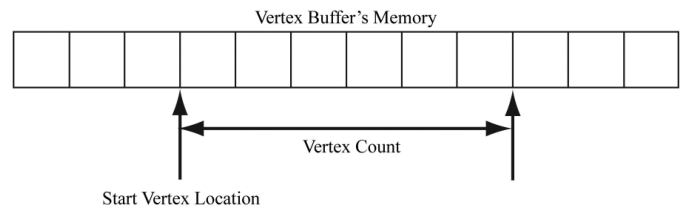
\includegraphics[width=\textwidth]{6-2}
    \centering
    \caption{StartVertexLocation 表示开始绘制的顶点缓冲区的第一个元素。VertexCountPerInstance 表示绘制顶点的个数。}
    \label{fig:6-2}
\end{figure}

DrawInstanced 方法没有制定顶点的基本类型。它们需要被绘制成点,线列表,还是三角列表?回忆5.5.2节,基本拓扑状态是通过 ID3D12GraphicsCommandList::IASetPrimitiveTopology 方法设置的。例:\\
\begin{lstlisting}
mCommandList->IASetPrimitiveTopology(D3D_PRIMITIVE_TOPOLOGY_TRIANGLELIST);
\end{lstlisting}
\end{flushleft}
\section{索引和索引缓冲区(Indices and Index Buffers)}
\begin{flushleft}
与顶点类似,为了让GPU访问索引数组,需要将索引数组放到GPU缓冲区资源中(ID3D12Resource)。我们将存储索引的缓冲区叫索引缓冲区(index buffer)。因为 d3dUtil::CreateDefaultBuffer 方法能通过 void* 作用于一般数据,我们同样使用该方法来创建索引缓冲区(或任何默认缓冲区)。\\
为了将索引缓冲区绑定到管道,我们需要为索引缓冲区资源创建一个索引缓冲区视图。 与顶点缓冲区视图一样,我们不需要一个描述符堆用于索引缓冲区视图。 索引缓冲区视图由D3D12\_INDEX\_BUFFER\_VIEW结构表示:\\
\begin{lstlisting}
typedef struct D3D12_INDEX_BUFFER_VIEW
{
    D3D12_GPU_VIRTUAL_ADDRESS bufferLocation;
    UINT SizeInBytes;
    DXGI_FORMAT Format;
} D3D12_INDEX_BUFFER_VIEW;
\end{lstlisting}
1. BufferLocation: 创建视图的顶点缓冲区资源的虚拟地址。 我们可以使用ID3D12Resource :: GetGPUVirtualAddress方法来获取它。\\
2. SizeInBytes:从BufferLocation开始在索引缓冲区中查看的字节数。\\
3. Format:索引的格式必须是16位索引的 DXGI\_FORMAT\_R16\_UINT 或32位索引的 DXGI\_FORMAT\_R32\_UINT。 如果索引值需要额外的32位范围,则应使用16位索引来减少内存和带宽,并仅使用32位索引。\\
~\\
就顶点缓冲区和其他Direct3D资源而言,在我们可以使用它之前,我们需要将它绑定到管道。 使用 ID3D12CommandList::SetIndexBuffer方法将索引缓冲区绑定到输入汇编程序阶段。 以下代码显示了如何创建一个定义多维数据集三角形的索引缓冲区,创建一个视图并将其绑定到管道:\\
\begin{lstlisting}
std::uint16_t indices[] = {
    // front face
    0, 1, 2,
    0, 2, 3,
    
    // back face
    4, 6, 5,
    4, 7, 6,
    
    // left face
    4, 6, 1,
    4, 1, 0,
    
    // right face
    3, 2, 6,
    3, 6, 7,
    
    // top face
    1, 5, 6,
    1, 6, 2,
    
    // bottom face
    4, 0, 3,
    4, 3, 7
};

const UINT ibByteSize = 36 * sizeof(std::uint16_t);

ComPtr<ID3D12Resource> IndexBufferGPU = nullptr;
ComPtr<ID3D12Resource> IndexBufferUploader = nullptr;
IndexBufferGPU = d3dUtil::CreateDefaultBuffer(md3dDevice.Get(), 
                       mCommandList.Get(), indices, ibByteSize, 
                       IndexBufferUploader);

D3D12_INDEX_BUFFER_VIEW ibv;
ibv.BufferLocation = IndexBufferGPU->GetGPUVirtualAddress();
ibv.Format = DXGI_FORMAT_R16_UINT;
ibv.SizeInBytes = ibByteSize;

mCommandList->IASetIndexBuffer(&ibv);
\end{lstlisting}
最后,使用索引时,用 ID3D12GraphicsCommandList::DrawIndexedInstanced 方法,而不是 DrawInstanced:\\
\begin{lstlisting}
void ID3D12GraphicsCommandList::DrawIndexedInstanced(
    UINT IndexCountPerInstance,
    UINT InstanceCount,
    UINT StartIndexLocation,
    INT BaseVertexLocation,
    UINT StartInstanceLocation);
\end{lstlisting}
1. IndexCountPerInstance:要绘制的索引数量(每个实例)。\\
2. InstanceCount:用于称为实例的高级技术; 现在,将其设置为1,因为我们只绘制一个实例。\\
3. StartIndexLocation:索引缓冲区中的一个元素索引,标志着开始读取索引的起始点。\\
4. BaseVertexLocation:在获取顶点之前,要将此整数值添加到此绘图调用使用的索引中。\\
5. StartInstanceLocation:用于称为实例的高级技术, 目前指定为0。\\
~\\
为了说明这些参数,请考虑以下情况。假设我们有三个对象:一个球体,一个盒子和一个圆柱体。首先,每个对象都有自己的顶点缓冲区和自己的索引缓冲区。每个本地索引缓冲区中的索引都与相应的本地顶点缓冲区有关。现在假设我们将球体,盒子和圆柱体的顶点和索引连接成一个全局顶点和索引缓冲区,如图\ref{fig:6-3}所示。 (可能会连接顶点和索引缓冲区,因为在更改顶点和索引缓冲区时会有一些API开销,这很可能不是瓶颈,但是如果有许多小的顶点和索引缓冲区可以很容易地合并,值得这样做是出于性能方面的原因。)在这个串联之后,索引不再是正确的,因为它们存储索引位置相对于它们相应的本地顶点缓冲区而不是全局索引位置;因此需要重新计算索引以正确地将索引指向全局顶点缓冲区。原始盒子索引是在假设盒子的顶点贯穿索引的情况下计算出来的 0, 1, ..., numBoxVertices-1\\
但是合并之后,就成为:\\
\begin{lstlisting}
firstBoxVertexPos,
firstBoxVertexPos+1,
...,
firstBoxVertexPos+numBoxVertices-1
\end{lstlisting}
 
\begin{figure}[h]
    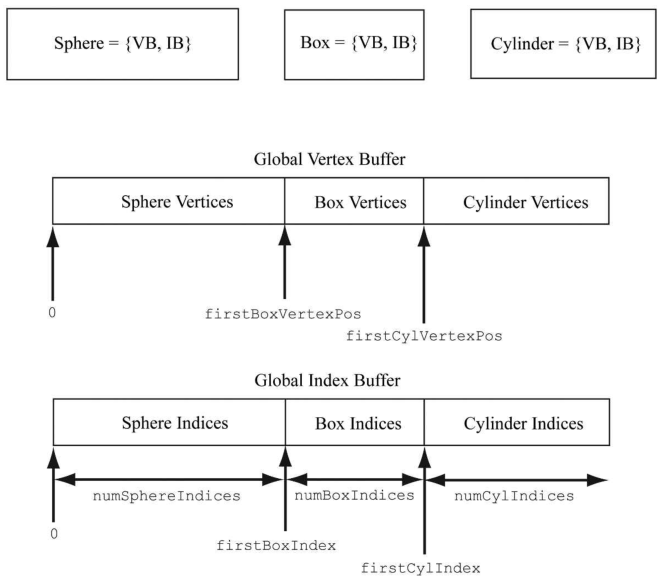
\includegraphics[width=\textwidth]{6-3}
    \centering
    \caption{将几个顶点缓冲区连接成一个大的顶点缓冲区,并将几个索引缓冲区连接成一个大的索引缓冲区。}
    \label{fig:6-3}
\end{figure}

因此,要更新索引,我们需要为每个Box索引添加第一个 firstBoxVertexPos。 同样,我们需要为每个柱面索引添加 firstCylVertexPos。 请注意,球体的指标不需要改变(因为第一个球体顶点位置为零)。 让我们把对象的第一个顶点相对于全局顶点缓冲区的位置称为它的基本顶点位置。 通常,对象的新索引是通过将其基本顶点位置添加到每个索引来计算的。 我们可以让 Direct3D 通过将基本顶点位置传递给 DrawIndexedInstanced 的第四个参数来完成它,而不必自己计算新的索引。\\
然后我们可以用以下三个调用一个接一个地绘制球体,盒子和圆柱体:\\
\begin{lstlisting}
mCmdList->DrawIndexedInstanced(numSphereIndices, 1, 
                               0, 0, 0);
mCmdList->DrawIndexedInstanced(numBoxIndices, 1, 
                               firstBoxIndex, firstBoxVertexPos, 0);
mCmdList->DrawIndexedInstanced(numCylIndices, 1, 
                               firstCylIndex, firstCylVertexPos, 0);
\end{lstlisting}
下一章(chapter)"Shapes"代码样例就使用了这样的技术。
\end{flushleft}

\clearpage
\section{顶点着色器例子(Example Vertex Shader)}
\begin{flushleft}
下面是简单顶点着色器的实现(回忆5.6节):
\end{flushleft}
\begin{lstlisting}
cbuffer cbPerObject : register(b0)
{
    float4x4 gWorldViewProj;
};

void VS(float3 iPosL      : POSITION,
        float4 iColor     : COLOR,
        out float4 oPosH  : SV_POSITION,
        out float4 oColor : COLOR)
{
    // Transform to homogeneous clip space.
    oPosH = mul(float4(iPosL, 1.0f), gWorldViewProj);
    // Just pass vertex color into the pixel shader.
    oColor = iColor;
}
\end{lstlisting}
\begin{flushleft}
着色器使用一种称为高级着色语言(HLSL)的语言编写,它具有与 C++ 类似的语法,因此很容易学习。 附录B提供了对HLSL的简明参考。 我们教授HLSL和编程着色器的方法将以示例为基础。 也就是说,随着本书的进展,我们将介绍我们需要的任何新的HLSL概念,以便实现手头的演示。 着色器通常用基于文本的文件编写,扩展名为.hlsl。\\
顶点着色器是名为VS的函数。 请注意,您可以为顶点着色器指定任何有效的函数名称。 该顶点着色器有四个参数; 前两个是输入参数,后两个是输出参数(由out关键字表示)。 HLSL没有引用或指针,因此要从函数返回多个值,您需要使用结构或输出参数。 在HLSL中,函数始终内联。\\
前两个输入参数构成顶点着色器的输入签名(input signature),并对应于我们用于绘制的自定义顶点结构中的数据成员。 参数语义“:POSITION”和“:COLOR”用于将顶点结构中的元素映射到顶点着色器输入参数,如图\ref{fig:6-4}所示。
\end{flushleft}
\begin{figure}[h]
    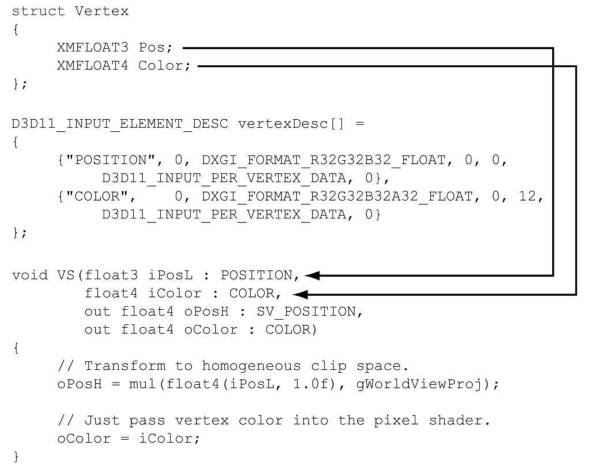
\includegraphics[width=\textwidth]{6-4}
    \centering
    \caption{每个顶点元素都有一个由 D3D12\_INPUT\_ELEMENT\_DESC 数组指定的相关语义。 顶点着色器的每个参数也具有附加的语义。语义用于将顶点元素与顶点着色器参数进行匹配。}
    \label{fig:6-4}
\end{figure}

\begin{flushleft}
输出参数也有附加的语义(“:SV\_POSITION”和“:COLOR”)。 这些用于将顶点着色器输出映射到下一级的相应输入(几何着色器或像素着色器)。 请注意,SV\_POSITION 语义是特殊的(SV代表系统值)。 它用于表示在同构剪辑空间中保存顶点位置的顶点着色器输出元素。 我们必须将SV\_POSITION语义附加到位置输出,因为GPU需要知道这个值,因为它涉及其他属性不涉及的操作,例如剪切,深度测试和光栅化。 非系统值的输出参数的语义名称可以是任何有效的语义名称。\\
第一行通过乘以4x4矩阵 gWorldViewProj 将顶点位置从局部空间转换为齐次剪辑空间:\\
\end{flushleft}
\begin{lstlisting}
// Transform to homogeneous clip space.
oPosH = mul(float4(iPosL, 1.0f), gWorldViewProj);
\end{lstlisting}
\begin{flushleft}
构造函数语法 float4(iPosL,1.0f) 构造一个4D向量,相当于 float4(iPosL.x,iPosL.y,iPosL.z,1.0f); 因为我们知道顶点的位置是点而不是矢量,所以我们在第四个分量中放置 1(w = 1)。float2 和 float3 类型分别代表2D和3D向量。 矩阵变量 gWorldViewProj 存在于所谓的常量缓冲区中,这将在下一节中讨论。 内置函数 mul 用于向量矩阵乘法。顺便提一下,对于不同大小的矩阵乘法,mul 函数是重载(overloaded)的; 例如,您可以使用它来乘以两个4x4矩阵,两个3x3矩阵,或1x3矢量和3x3矩阵。 着色器主体中的最后一行只是将输入颜色复制到输出参数,以便将颜色输入到管道的下一个阶段:\\
\end{flushleft}
\begin{lstlisting}
oColor = iColor;
\end{lstlisting}
\begin{flushleft}
我们可以使用返回类型和输入签名(input signature)的结构(而不是长参数列表)等效地重写上面的顶点着色器:\\
\end{flushleft}
\begin{lstlisting}
cbuffer cbPerObject : register(b0)
{
    float4x4 gWorldViewProj;
};
struct VertexIn
{
    float3 PosL : POSITION;
    float4 Color : COLOR;
};
struct VertexOut
{
    float4 PosH : SV_POSITION;
    float4 Color : COLOR;
};
VertexOut VS(VertexIn vin)
{
    VertexOut vout;
    // Transform to homogeneous clip space.
    vout.PosH = mul(float4(vin.PosL, 1.0f), gWorldViewProj);
    // Just pass vertex color into the pixel shader.
    vout.Color = vin.Color;
    return vout;
}
\end{lstlisting}
\begin{flushleft}
NOTICE: 如果没有几何着色器(第12章中介绍几何着色器),则顶点着色器必须使用 SV\_POSITION 语义输出齐次剪辑空间中的顶点位置,因为这是硬件在离开顶点时期望顶点所在的空间 着色器(如果没有几何着色器)。 如果存在几何着色器,则输出齐次剪辑空间位置的作业可以推迟到几何着色器。\\
~\\
NOTICE: 顶点着色器(或几何着色器)不执行透视分割; 它只是投影矩阵部分。 透视分割将稍后由硬件完成。
\end{flushleft}

\subsection{输入布局描述和输入签名链接(Input Layout Description and Input Signature Linking)}
\begin{flushleft}
从图\ref{fig:6-4}中可以看出,提供给管道的顶点属性之间存在链接,这是由输入布局描述定义的。 如果您输入的顶点不提供顶点着色器所需的所有输入,则会产生错误。 例如,以下顶点着色器输入签名和顶点数据不兼容:\\
\end{flushleft}
\begin{lstlisting}
//––––—
// C++ app code
//––––—
struct Vertex
{
    XMFLOAT3 Pos;
    XMFLOAT4 Color;
};
D3D12_INPUT_ELEMENT_DESC desc[] =
{
    {"POSITION", 0, DXGI_FORMAT_R32G32B32_FLOAT, 0, 0,
                 D3D12_INPUT_PER_VERTEX_DATA, 0},
    {"COLOR",    0, DXGI_FORMAT_R32G32B32A32_FLOAT, 0, 12,
                 D3D12_INPUT_PER_VERTEX_DATA, 0}
};
//––––—
// Vertex shader
//––––—
struct VertexIn
{
    float3 PosL   : POSITION;
    float4 Color  : COLOR;
    float3 Normal : NORMAL;
};
struct VertexOut
{
    float4 PosH  : SV_POSITION;
    float4 Color : COLOR;
};
VertexOut VS(VertexIn vin) {...}
\end{lstlisting}

\begin{flushleft}
正如我们将在6.9节中看到的那样,当我们创建一个 ID3D12PipelineState 对象时,我们必须同时指定输入布局描述和顶点着色器。 然后,Direct3D将验证输入布局描述和顶点着色器是否兼容。\\
顶点数据和输入签名不需要完全匹配。 所需要的是顶点数据提供顶点着色器期望的所有数据。 因此,允许顶点数据提供顶点着色器不使用的附加数据。 也就是说,以下是兼容的:
\end{flushleft}

\begin{lstlisting}
//––––—
// C++ app code
//––––—
struct Vertex
{
   XMFLOAT3 Pos;
   XMFLOAT4 Color;
   XMFLOAT3 Normal;
};
D3D12_INPUT_ELEMENT_DESC desc[] =
{
    {"POSITION", 0, DXGI_FORMAT_R32G32B32_FLOAT, 0, 0,
                 D3D12_INPUT_PER_VERTEX_DATA, 0},
    {"COLOR",    0, DXGI_FORMAT_R32G32B32A32_FLOAT, 0, 12,
                 D3D12_INPUT_PER_VERTEX_DATA, 0},
    {"NORMAL",   0, DXGI_FORMAT_R32G32B32_FLOAT, 0, 28,
                 D3D12_INPUT_PER_VERTEX_DATA, 0 }
};
//––––—
// Vertex shader
//––––—
struct VertexIn
{
    float3 PosL  : POSITION;
    float4 Color : COLOR;
};
struct VertexOut
{
    float4 PosH  : SV_POSITION;
    float4 Color : COLOR;
};
VertexOut VS(VertexIn vin) {...}
\end{lstlisting}
\begin{flushleft}
现在考虑顶点结构和输入签名具有匹配的顶点元素的情况,但颜色属性的类型是不同的:\\
\end{flushleft}
\begin{lstlisting}
//––––—
// C++ app code
//––––—
struct Vertex
{
    XMFLOAT3 Pos;
    XMFLOAT4 Color;
};
D3D12_INPUT_ELEMENT_DESC desc[] =
{
    {"POSITION", 0, DXGI_FORMAT_R32G32B32_FLOAT, 0, 0,
                 D3D12_INPUT_PER_VERTEX_DATA, 0},
    {"COLOR",    0, DXGI_FORMAT_R32G32B32A32_FLOAT, 0, 12,
                 D3D12_INPUT_PER_VERTEX_DATA, 0}
};
//––––—
// Vertex shader
//––––—
struct VertexIn
{
    float3 PosL : POSITION;
    int4 Color  : COLOR;
};
struct VertexOut
{
    float4 PosH  : SV_POSITION;
    float4 Color : COLOR;
};
VertexOut VS(VertexIn vin) {...}
\end{lstlisting}

\begin{flushleft}
这实际上是合法的,因为Direct3D允许重新解释输入寄存器中的位。 但是,VC++调试输出窗口提供以下警告:\\
\end{flushleft}
\begin{lstlisting}
D3D12 WARNING: ID3D11Device::CreateInputLayout: The
provided input signature expects to read an element with
SemanticName/Index: ‘COLOR’/0 and component(s) of the
type ‘int32’. However, the matching entry in the Input
Layout declaration, element[1], specifies mismatched
format: ‘R32G32B32A32_FLOAT’. This is not an error, since
behavior is well defined: The element format determines
what data conversion algorithm gets applied before it
shows up in a shader register. Independently, the shader
input signature defines how the shader will interpret the
data that has been placed in its input registers, with no
change in the bits stored. It is valid for the
application to reinterpret data as a different type once
it is in the vertex shader, so this warning is issued
just in case reinterpretation was not intended by the
author.
\end{lstlisting}

\begin{figure}[h]
	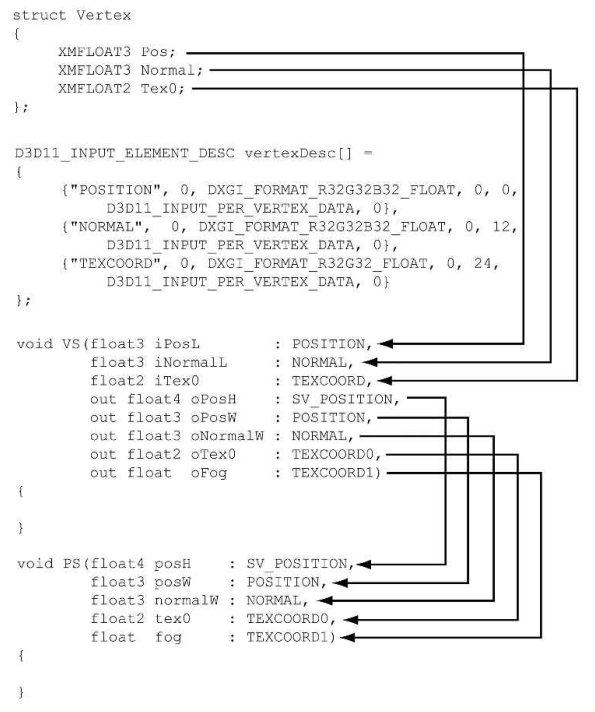
\includegraphics[width=\textwidth]{6-5}
	\centering
	\caption{每个顶点元素都有一个由 D3D12\_INPUT\_ELEMENT\_DESC 数组指定的相关语义。 顶点着色器的每个参数也具有附加的语义。 语义用于将顶点元素与顶点着色器参数进行匹配。 同样,顶点着色器的每个输出都有一个附加的语义,每个像素着色器输入参数都有一个附加的语义。 这些语义用于将顶点着色器输出映射到像素着色器输入参数。}
	\label{fig:6-5}
\end{figure}

\section{像素着色器例子(Example Pixel Shader)}
\begin{flushleft}
如5.10.3节中所述,在光栅化期间,从顶点着色器(或几何着色器)输出的顶点属性在三角形的像素上进行插值。 然后将插值作为输入(5.11节)输入像素着色器。 假设没有几何着色器,图\ref{fig:6-5}说明了到目前为止顶点数据的路径。
\end{flushleft}

\begin{flushleft}
像素着色器就像顶点着色器,因为它是为每个像素片段执行的函数。 给定像素着色器输入,像素着色器的作用是计算像素片段的颜色值。 我们注意到像素片段可能无法存活并使其进入后缓冲区; 例如,它可能被剪裁在像素着色器中(HLSL包含clip 函数,可以丢弃进一步处理的像素片段),被另一个具有较小深度值的像素片段遮挡,或者像素片段可能被稍后丢弃 管道测试就像模板缓冲测试一样。 因此,后缓冲器上的像素可以具有多个像素片段候选; 这是“像素片段”和“像素”的含义之间的区别,尽管有时这些术语可以互换使用,但上下文通常会明确其含义。\\
~\\
NOTICE: 作为硬件优化,在将像素片段设置到像素着色器之前(例如,early-z rejection),可能会使管道拒绝像素片段。 这是首先进行深度测试的地方,并且如果确定像素片段被深度测试遮挡,则跳过像素着色器。 但是,有些情况可能会禁用early-z rejection优化。 例如,如果像素着色器修改像素的深度,则必须执行像素着色器,因为如果像素着色器更改像素着色器,我们实际上不知道像素着色器的深度。\\
~\\
下面是一个简单的像素着色器,它对应于§6.4中给出的顶点着色器。 为完整起见,再次显示顶点着色器。\\
\end{flushleft}
\begin{lstlisting}
cbuffer cbPerObject : register(b0)
{
    float4x4 gWorldViewProj;
};
void VS(float3 iPos : POSITION, 
        float4 iColor : COLOR,
        out float4 oPosH : SV_POSITION,
        out float4 oColor : COLOR)
{
    // Transform to homogeneous clip space.
    oPosH = mul(float4(iPos, 1.0f), gWorldViewProj);
    // Just pass vertex color into the pixel shader.
    oColor = iColor;
}

float4 PS(float4 posH  : SV_POSITION, 
          float4 color : COLOR) : SV_Target
{
    return pin.Color;
}
\end{lstlisting}
\begin{flushleft}
在此示例中,像素着色器仅返回插值颜色值。 请注意,像素着色器输入与顶点着色器输出完全匹配; 这是一项要求。 像素着色器返回4D颜色值,函数参数列表后面的SV\_TARGET语义指示返回值类型应与渲染目标格式匹配。\\
我们可以使用输入/输出结构等效地重写上面的顶点和像素着色器。 符号的不同之处在于我们将语义附加到输入/输出结构的成员,并且我们使用return语句来输出而不是输出参数。
\end{flushleft}
\begin{lstlisting}
cbuffer cbPerObject : register(b0)
{
    float4x4 gWorldViewProj;
};
struct VertexIn
{
    float3 Pos   : POSITION;
    float4 Color : COLOR;
};
struct VertexOut
{
    float4 PosH : SV_POSITION;
    float4 Color : COLOR;
};
VertexOut VS(VertexIn vin)
{
    VertexOut vout;
    // Transform to homogeneous clip space.
    vout.PosH = mul(float4(vin.Pos, 1.0f), gWorldViewProj);
    // Just pass vertex color into the pixel shader.
    vout.Color = vin.Color;
    return vout;
}
float4 PS(VertexOut pin) : SV_Target
{
    return pin.Color;
}
\end{lstlisting}

\section{常量缓冲区(Constant Buffers)}
\subsection{创建常量缓冲区(Creating Constant Buffers)}
\begin{flushleft}
常量缓冲区是GPU资源(ID3D12Resource)的一个例子,其数据内容可在着色器程序中引用。 正如我们将在本书中学习的那样,着色器程序中也可以引用纹理和其他类型的缓冲区资源。 6.4节中的示例顶点着色器的代码如下:
\begin{lstlisting}
cbuffer cbPerObject: register(b0)
{
    float4x4 gWorldViewProj;
}
\end{lstlisting}
此代码引用一个名为cbPerObject的cbuffer对象(常量缓冲区)。 在这个例子中,常量缓冲区存储一个名为gWorldViewProj的4x4矩阵,表示用于将点从本地空间转换为同类剪辑空间的组合世界,视图和投影矩阵。 在HLSL中,4x4矩阵由内置的float4x4类型声明; 要声明3x4矩阵和2x4矩阵,例如,您将分别使用float3x4和float2x2类型。\\
与顶点和索引缓冲区不同,常量缓冲区通常由CPU每帧更新一次。 例如,如果摄像机每帧移动一次,则每帧必须使用新的视图矩阵更新常量缓冲区。 因此,我们在上传堆而不是默认堆中创建常量缓冲区,以便我们可以从CPU更新内容。\\
常量缓冲区也有特殊的硬件要求,它们的大小必须是最小硬件分配大小(256字节)的倍数。\\
通常我们需要多个相同类型的常量缓冲区。 例如,上面的常量缓冲区cbPerObject存储每个对象不同的常量,所以如果我们有n个对象,那么我们将需要n个这种类型的常量缓冲区。 以下代码显示了我们如何创建一个存储NumElements多个常量缓冲区的缓冲区:
\begin{lstlisting}
struct ObjectConstants
{
    DirectX::XMFLOAT4X4 WorldViewProj = MathHelper::Identity4x4();
};

UINT elementByteSize = d3dUtil::CalcConstantBufferByteSize(
                                     sizeof(ObjectConstants));

ComPtr<ID3D12Resource> mUploadCBuffer;
device->CreateCommittedResource(
    &CB3DX12_HEAP_PROPERTIES(D3D12_HEAP_TYPE_UPLOAD), 
    D3D12_HEAP_FLAG_NONE, 
    &CD3DX12_RESOURCE_DESC::Buffer(elementByteSize * NumElements),
    D3D12_RESOURCE_STATE_GENERIC_READ,
    nullptr, 
    IID_PPV_ARGS(&mUploadCBuffer));
\end{lstlisting}
我们可以将mUploadCBuffer视为存储ObjectConstants类型的常量缓冲区数组(使用填充为256的倍数)。 当需要绘制一个对象时,我们只需将一个常量缓冲区视图(CBV)绑定到缓冲区的一个存储该对象常量的子区域。 请注意,我们经常会调用缓冲区mUploadCBuffer作为常量缓冲区,因为它存储了一个常量缓冲区数组。\\
工具函数 d3dUtil::CalcConstantBufferByteSize 会进行算术运算将缓冲区的字节大小舍入为最小硬件分配大小(256字节)的倍数:\\
\begin{lstlisting}
static UINT CalcConstantBufferByteSize(UINT byteSize)
{
    // Constant buffers must be a multiple of the minimum hardware
    // allocation size (usually 256 bytes).  So round up to nearest
    // multiple of 256.  We do this by adding 255 and then masking off
    // the lower 2 bytes which store all bits < 256.
    // Example: Suppose byteSize = 300.
    // (300 + 255) & ~255
    // 555 & ~255
    // 0x022B & ~0x00ff
    // 0x022B & 0xff00
    // 0x0200
    // 512
    return (byteSize + 255) & ~255;
}
\end{lstlisting}
NOTICE: 即使我们以256的倍数分配常量数据,也不需要在HLSL结构中明确填充相应的常量数据,因为它是隐式完成的:\\
\begin{lstlisting}
// Implicitly padded to 256 bytes.
cbuffer cbPerObject : register(b0)
{
    float4x4 gWorldViewProj;
};

// Explicitly padded to 256 bytes.
cbuffer cbPerObject : register(b0)
{
    float4x4 gWorldViewProj;
    float4x4 Pad0;
    float4x4 Pad1;
    float4x4 Pad1;
}
\end{lstlisting}
NOTICE: 为避免处理将常量缓冲区元素舍入为256字节的倍数,可以明确地将所有常量缓冲区结构填充为256字节的整数倍。\\
~\\
Direct3D 12推出了着色器模型5.1。 Shader model 5.1引入了一种替代HLSL语法来定义一个常量缓冲区,如下所示:\\
\begin{lstlisting}
struct ObjectConstants
{
    float4x4 gWorldViewProj;
    uint matIndex;
};
ConstantBuffer<ObjectConstants> gObjConstants : register(b0);
\end{lstlisting}
这里常量缓冲区的数据元素只是在一个单独的结构中定义,然后从该结构创建一个常量缓冲区。 然后使用数据成员语法在着色器中访问常量缓冲区的字段:\\
\begin{lstlisting}
uint index = gObjConstants.matIndex;
\end{lstlisting}
\end{flushleft}

\subsection{更新常量缓冲区(Updating Constant Buffers)}
\begin{flushleft}
因为一个常量缓冲区是由 D3D12\_HEAP\_TYPE\_UPLOAD 的堆类型创建的,所以我们能从CPU上传常量缓冲区资源。为了做到这一点,要先通过 Map 方法获得资源数据的指针:\\
\begin{lstlisting}
ComPtr<ID3D12Resource> mUploadBuffer;
BYTE* mMappedData = nullptr;
mUploadBuffer->Map(0, nullptr, reinterpret_cast<void**>(&mMappedData));
\end{lstlisting}
第一个参数表示要映射的子资源索引。 对于一个缓冲区,唯一的子资源就是缓冲区本身,所以我们将其设置为0.第二个参数是一个指向D3D12\_RANGE结构的可选指针,该结构描述要映射的内存范围; 指定null映射整个资源。 第三个参数返回一个指向映射数据的指针。 要将数据从系统内存复制到常量缓冲区,我们只需执行一个memcpy即可:\\
\begin{lstlisting}
memcpy(mMappedData, &data, dataSizeInBytes);
\end{lstlisting}
当我们处理完常量缓冲区后,我们应该在释放内存之前 Unmap 它:\\
\begin{lstlisting}
if (mUploadBuffer != nullptr)
    mUploadBuffer->Unmap(0, nullptr);
mMappedData = nullptr;
\end{lstlisting}
Unmap 的第一个参数表示要映射的子资源索引,对于 buffer,这里设为0。第二个参数是一个指向D3D12\_RANGE结构的可选指针,该结构描述要unmap的内存范围; 指定null,unmap 整个资源。
\end{flushleft}

\subsection{上传缓冲区帮助工具(Upload Buffer Helper)}
\begin{flushleft}
在上传缓冲区周围构建一个简单的包装器很方便。 我们在UploadBuffer.h中定义了以下类,以便更轻松地处理上传缓冲区。 它为我们处理上传缓冲区资源的构建和销毁,处理映射和取消映射资源,并提供CopyData方法来更新缓冲区中的特定元素。 当我们需要从CPU更改上传缓冲区的内容时(例如,当视图矩阵发生变化时),我们使用CopyData方法。 请注意,这个类可以用于任何上传缓冲区,不一定是一个常量缓冲区。 但是,如果我们将它用于常量缓冲区,则需要通过isConstantBuffer构造函数参数进行指示。 如果它正在存储一个常量缓冲区,那么它会自动填充内存,使每个常量缓冲区为256字节的倍数。
\end{flushleft}
\begin{lstlisting}
template<typename T>
class UploadBuffer
{
public:
    UploadBuffer(ID3D12Device* device, UINT elementCount, 
                 bool isConstantBuffer) 
                 : mIsConstantBuffer(isConstantBuffer)
    {
        mElementByteSize = sizeof(T);

        // Constant buffer elements need to be multiples of 256 bytes.
        // This is because the hardware can only view constant data 
        // at m*256 byte offsets and of n*256 byte lengths. 
        // typedef struct D3D12_CONSTANT_BUFFER_VIEW_DESC {
        // UINT64 OffsetInBytes; // multiple of 256
        // UINT   SizeInBytes;   // multiple of 256
        // } D3D12_CONSTANT_BUFFER_VIEW_DESC;
        if(isConstantBuffer)
            mElementByteSize = d3dUtil::CalcConstantBufferByteSize(
                                                         sizeof(T));

        ThrowIfFailed(device->CreateCommittedResource(
            &CD3DX12_HEAP_PROPERTIES(D3D12_HEAP_TYPE_UPLOAD),
            D3D12_HEAP_FLAG_NONE,
            &CD3DX12_RESOURCE_DESC::Buffer(mElementByteSize*elementCount),
            D3D12_RESOURCE_STATE_GENERIC_READ,
            nullptr,
            IID_PPV_ARGS(&mUploadBuffer)));

        ThrowIfFailed(mUploadBuffer->Map(0, nullptr, 
                          reinterpret_cast<void**>(&mMappedData)));

        // We do not need to unmap until we are done with the resource.
        // However, we must not write to
        // the resource while it is in use by the GPU 
        // (so we must use synchronization techniques).
    }

    UploadBuffer(const UploadBuffer& rhs) = delete;
    UploadBuffer& operator=(const UploadBuffer& rhs) = delete;
    ~UploadBuffer()
    {
        if(mUploadBuffer != nullptr)
            mUploadBuffer->Unmap(0, nullptr);

        mMappedData = nullptr;
    }

    ID3D12Resource* Resource()const
    {
        return mUploadBuffer.Get();
    }

    void CopyData(int elementIndex, const T& data)
    {
        memcpy(&mMappedData[elementIndex*mElementByteSize], &data, 
                                                         sizeof(T));
    }

private:
    Microsoft::WRL::ComPtr<ID3D12Resource> mUploadBuffer;
    BYTE* mMappedData = nullptr;

    UINT mElementByteSize = 0;
    bool mIsConstantBuffer = false;
};
\end{lstlisting}
\begin{flushleft}
通常情况下,对象的世界矩阵在移动/旋转/缩放时会发生变化,视图矩阵会在摄像机移动/旋转时发生变化,并且在窗口大小调整时投影矩阵发生变化。 在本章的演示中,我们允许用户使用鼠标旋转和移动摄像头,并且我们在更新函数的每一帧中使用新的视图矩阵更新组合的世界视图投影矩阵:
\end{flushleft}
\begin{lstlisting}
void BoxApp::OnMouseMove(WPARAM btnState, int x, int y)
TODO....
\end{lstlisting}

\subsection{常量缓冲区描述符(Constant Buffer Descriptor)}
\begin{flushleft}
回想一下4.1.6节,我们通过描述符对象将资源绑定到渲染管道。 到目前为止,我们已经使用渲染目标,深度/模板缓冲区,顶点和索引缓冲区的描述符/视图。 我们还需要描述符来将常量缓冲区绑定到管道。 常量缓冲区描述符位于D3D12\_DESCRIPTOR\_HEAP\_TYPE\_CBV\_SRV\_UAV类型的描述符堆中。 这样的堆可以存储常量缓冲区,着色器资源和无序访问描述符的混合。 为了存储这些新类型的描述符,我们需要创建一个新的描述符堆类型:\\
\end{flushleft}
\begin{lstlisting}
D3D12_DESCRIPTOR_HEAP_DESC cbvHeapDesc;
cbvHeapDesc.NumDescriptors = 1;
cbvHeapDesc.Type = D3D12_DESCRIPTOR_HEAP_TYPE_CBV_SRV_UAV;
cbvHeapDesc.Flags = D3D12_DESCRIPTOR_HEAP_FLAG_SHADER_VISIBLE;
cbvHeapDesc.NodeMask = 0;

ComPtr<ID3D12DescriptorHeap> mCbvHeap;
md3dDevice->CreateDescriptorHeap(&cbvHeapDesc, IID_PPV_ARGS(&mCbvHeap));
\end{lstlisting}
\begin{flushleft}
这段代码与我们如何创建渲染目标和深度/模板缓冲区描述符堆相似。 然而,一个重要的区别是我们指定了D3D12\_DESCRIPTOR\_HEAP\_FLAG\_SHADER\_VISIBLE标志来表示这些描述符将被着色器程序访问。 在4.1.6节的演示中,我们没有SRV或UAV描述符,我们只绘制一个对象; 因此,我们只需要1个描述符来存储1个CBV。\\
通过填写一个D3D12\_CONSTANT\_BUFFER\_VIEW\_DESC实例并调用ID3D12Device::CreateConstantBufferView来创建一个常量缓冲区视图:\\
\end{flushleft}
\begin{lstlisting}
// Constant data per-object.
struct ObjectConstants
{
    XMFLOAT4X4 WorldViewProj = MathHelper::Identity4x4();
};

// Constant buffer to store the constants of n object.
std::unique_ptr<UploadBuffer<ObjectConstants>> mObjectCB = nullptr;
mObjectCB = std::make_unique<UploadBuffer<ObjectConstants>>(
                                        md3dDevice.Get(), n, true);

UINT objCBByteSize = d3dUtil::CalcConstantBufferByteSize(
                                           sizeof(ObjectConstants));

// Address to start of the buffer (0th constant buffer).
D3D12_CPU_VIRTUAL_ADDRESS cbAddress = mObjectCB->Resource()
                                          ->GetGPUVirtualAddress();

// Offset to the ith object constant buffer in the buffer.
int boxCBufIndex = i;
cbAddress += boxCBufIndex * objCBByteSize;

D3D12_CONSTANT_BUFFER_VIEW_DESC cbvDesc;
cbvDesc.BufferLocation = cbAddress;
cbvDesc.SizeInBytes = d3dUtil::CalcConstantBufferByteSize(
                                           sizeof(ObjectConstants));

md3dDevice->CreateConstantBufferView(&cbvDesc, mCbvHeap
                             ->GetCPUDescriptorHandleForHeapStart());
\end{lstlisting}
\begin{flushleft}
D3D12\_CONSTANT\_BUFFER\_VIEW\_DESC 结构描述了要绑定到HLSL常量缓冲区结构的常量缓冲区资源的子集。 如前所述,通常一个常量缓冲区存储n个对象的每个对象常量数组,但我们可以通过使用 BufferLocation 和 SizeInBytes 来获取第i个对象常量数据的视图。 由于硬件要求,D3D12\_CONSTANT\_BUFFER\_VIEW\_DESC::SizeInBytes 和D3D12\_CONSTANT\_BUFFER\_VIEW\_DESC::OffsetInBytes 成员必须为256个字节的倍数。 例如,如果您指定了64,那么您将得到以下调试错误:\\
\end{flushleft}
\begin{lstlisting}
D3D12 ERROR: ID3D12Device::CreateConstantBufferView: 
             SizeInBytes of 64 is invalid. 
             Device requires SizeInBytes be multiple of 256.

D3D12 ERROR: ID3D12Device::CreateConstantBufferView: 
             OffsetInBytes of 64 is invalid. 
             Device requires OffsetInBytes be a multiple of 256.
\end{lstlisting}

\subsection{根签名和描述符表(Root Signature and Descriptor Tables)}
\begin{flushleft}
通常,不同的着色器程序会希望在执行绘制调用之前将不同的资源绑定到渲染管道。 资源被绑定到特定的寄存器插槽,在那里它们可以被着色器程序访问。 例如,以前的顶点和像素着色器只需要一个常量缓冲区被绑定到寄存器b0。 本书稍后将使用的更高级的顶点和像素着色器集合将期望将几个常量缓冲区,纹理和采样器绑定到各种寄存器槽:\\
\begin{lstlisting}
// Texture resourcce bound to texture register slot 0.
Texture2D gDiffuseMap : register(t0);

// Sampler resources bound to sampler register slots 0-5.
SamplerState gsamPointWrap        : register(s0);
SamplerState gsamPointClamp       : register(s1);
SamplerState gsamLinearWrap       : register(s2);
SamplerState gsamLinearClamp      : register(s3);
SamplerState gsamAnisotropicWrap  : register(s4);
SamplerState gsamAnisotropicClamp : register(s5);

// cbuffer resource bound to cbuffer register slots 0-2
cbuffer cbPerObject : register(b0)
{
    float4x4 gWorld;
    float4x4 gTexTransform;
};

// Constant data that varies per material.
cbuffer cbPass : register(b1)
{
    float4x4 gView;
    float4x4 gProj;
    [...] // Other fields omitted for brevity.
};

cbuffer cbMaterial : register(b2)
{
    float4   gDiffuseAlbedo;
    float3   gFresnelR0;
    float    gRoughness;
    float4x4 gMatTransform;
};
\end{lstlisting}
根签名定义了在绘制调用可以执行之前应用程序将绑定到渲染管道的资源以及这些资源被映射到着色器输入寄存器的位置。 根签名必须与将要使用的着色器兼容(即,根签名必须提供着色器期望在绘制调用执行之前绑定到渲染管道的所有资源); 这将在创建管道状态对象时进行验证(6.9节)。 不同的绘制调用可能会使用一组不同的着色器程序,这需要不同的根签名。\\
~\\
NOTICE: 如果我们将着色器程序看作函数,并将着色器期望的输入资源作为函数参数来考虑,那么根签名可以被认为是定义函数签名(因此称为根签名)。 通过绑定不同的资源作为参数,着色器输出将会不同。 所以,例如,顶点着色器将取决于输入到着色器的实际顶点以及绑定资源。\\
~\\
Direct3D中的根签名由ID3D12RootSignature接口表示。 它由一组根参数定义,这些参数描述了着色器对绘制调用所期望的资源。 根参数可以是根常量,根描述符或描述符表。 我们将在下一章讨论根常量和根描述符; 在本章中,我们将只使用描述符表。 描述符表指定描述符堆中描述符的连续范围。\\
下面的代码创建一个根签名,该签名具有一个根描述符表,该描述符表足够大以存储一个CBV(常量缓冲区视图):\\
\begin{lstlisting}
// Root parameter can be a table, root descriptor or root constants.
CD3DX12_ROOT_PARAMETER slotRootParameter[1];

// Create a single descriptor table of CBVs.
CD3DX12_DESCRIPTOR_RANGE cbvTable;
cbvTable.Init(
    D3D12_DESCRIPTOR_RANGE_TYPE_CBV,
    1,  // Number of descriptors in table
    0); // base shader register arguments are bound to 
        // for this root parameter

slotRootParameter[0].InitAsDescriptorTable(
    1,          // Number of ranges
    &cbvTable); // Pointer to array of ranges

// A root signature is an array of root parameters.
CD3DX12_ROOT_SIGNATURE_DESC rootSigDesc(1, 
    slotRootParameter, 0, nullptr, 
    D3D12_ROOT_SIGNATURE_FLAG_ALLOW_INPUT_ASSEMBLER_INPUT);

// create a root signature with a single slot with pints to a
// descriptor range consisting of a single constant buffer.
ComPtr<ID3DBlob> serializedRootSig = nullptr;
ComPtr<ID3DBlob> errorBlob = nullptr;

HRESULT hr = D3D12SerializeRootSignature(&rootSigDesc, 
    D3D_ROOT_SIGNATURE_VERSION_1,
    serializedRootSig.GetAddressOf(),
    errorBlob.GetAddressOf());

ThrowIfFailed(md3dDevice->CreateRootSignature(
    0,
    serializedRootSig->GetBufferPointer(),
    serializedRootSig->GetBufferSize(),
    IID_PPV_ARGS(&mRootSignature)));
\end{lstlisting}
下一章我们再解释 CD3DX12\_ROOT\_PARAMETER 和 CD3DX12\_DESCRIPTOR\_RANGE,现在仅理解如下代码:\\
\begin{lstlisting}
CD3DX12_ROOT_PARAMETER slotRootParameter[1];

CD3DX12_DESCRIPTOR_RANGE cbvTable;
cbvTable.Init(
    D3D12_DESCRIPTOR_RANGE_TYPE_CBV, // table type
    1,  // Number of descriptors in table
    0); // base shader register arguments are bound to 
        // for this root parameter

slotRootParameter[0].InitAsDescriptorTable(
    1,          // Number of ranges
    &cbvTable); // Pointer to array of ranges
\end{lstlisting}
创建一个根参数,该参数需要1个CBV的描述符表被绑定到常量缓冲寄存器0(即,HLSL代码中的寄存器(b0))。\\
~\\
NOTICE: 我们在本章中的根签名示例非常简单。 在本书中,我们将看到许多根签名的例子,并且它们会根据需要增加复杂性。
~\\
根签名仅定义应用程序将绑定到渲染管道的资源; 它实际上并没有做任何资源绑定。 一旦使用命令列表设置了根签名,我们使用ID3D12GraphicsCommandList::SetGraphicsRootDescriptorTable将描述符表绑定到管道:\\
\begin{lstlisting}
void ID3D12GraphicsCommandList::SetGraphicsRootDescriptorTable(
    UINT RootParameterIndex,
    D3D12_GPU_DESCRIPTOR_HANDLE BaseDescriptor);
\end{lstlisting}
1. RootParameterIndex: 设置根参数的索引。\\
2. BaseDescriptor: 处理堆中的描述符,指定要设置的表中的第一个描述符。 例如,如果根签名指定该表具有五个描述符,则将BaseDescriptor和堆中接下来的四个描述符设置为此根表。\\
以下代码将根签名和CBV堆设置为命令列表,并将描述符表设置为标识要绑定到管道的资源:\\
\begin{lstlisting}
mCommandList->SetGraphicsRootSignature(mRootSignature.Get());
ID3D12DescriptorHeap* descriptorHeaps[] = {mCbvHeap.Get()};
mCommandList->SetDescriptorHeaps(_countof(descriptorHeaps), descriptorHeaps);

// Offset the CBV we want to use for this draw call.
CD3DX12_GPU_DESCRIPTOR_HANDLE cbv(mCbvHeap->GetGPUDescriptorHandleForheapStart());
cbv.Offset(cbvIndex, mCbvSrvUavDescriptorSize);
mCommandList->SetGraphicsRootDescriptorTable(0, cbv);
\end{lstlisting}
~\\
NOTICE: 为了提高性能,请尽可能缩小根签名,并尽量减少每个渲染帧更改根签名的次数。\\
NOTICE: 只要内容的任何部分在绘图/分派调用之间发生变化,应用程序绑定的根签名(描述符表,根常量和根描述符)的内容就会自动得到D3D12驱动程序的版本控制。 所以每个绘图/分派都会得到一个独特的全套根签名状态。\\
NOTICE: 如果更改根签名,则会丢失所有现有的绑定。 也就是说,您需要重新绑定新根签名所需的所有资源。
\end{flushleft}

\section{编译着色器(Compiling Shaders)}
\begin{flushleft}
在Direct3D中,着色器程序必须首先编译为便携式字节码。 然后,图形驱动程序将获取该字节码并将其重新编译为系统GPU [ATI1]的最佳本机指令。 在运行时,我们可以使用以下函数编译着色器:\\
\begin{lstlisting}
HRESULT D3DCompileFromFile(
    LPCWSTR pFileName,
    const D3D_SHADER_MACRO *pDefines,
    ID3DInclude *pInclude,
    LPCSTR pEntrypoint,
    LPCSTR pTarget,
    UINT Flags1,
    UINT Flags2,
    ID3DBlob **ppCode,
    ID3DBlob **ppErrorMsgs);
\end{lstlisting}
1. pFileName: .hlsl 后缀的文件名称,该文件包含了需要编译的HLSL源代码。\\
2. pDefines: 不使用的高级选项; 请参阅SDK文档。 我们在本书中总是指定null。\\
3. pInclude: 不使用的高级选项; 请参阅SDK文档。 我们在本书中总是指定null。\\
4. pEntrypoint: 着色器入口点的函数名称。 一个.hlsl可以包含多个着色器程序(例如,一个顶点着色器和一个像素着色器),所以我们需要指定我们想要编译的特定着色器的入口点。\\
5. pTarget: 指定我们正在使用的着色器程序类型和版本的字符串。在本书中,我们的目标是版本5.0和5.1。\\
\begin{itemize}
  \item a) vs\_5\_0 和 vs\_5\_1: 顶点着色器(vertex shader) 5.0 和 5.1。
  \item b) hs\_5\_0 和 hs\_5\_1: 外壳着色器(hull shader) 5.0 和 5.1。
  \item c) ds\_5\_0 和 ds\_5\_1: 域着色器(domain shader) 5.0 和 5.1。
  \item c) gs\_5\_0 和 gs\_5\_1: 几何着色器(geometry shader) 5.0 和 5.1。
  \item c) ps\_5\_0 和 ps\_5\_1: 像素着色器(pixel shader) 5.0 和 5.1。
  \item c) cs\_5\_0 和 cs\_5\_1: 计算着色器(compute shader) 5.0 和 5.1。
\end{itemize}
5. Flags1: 用于指定应该如何编译着色器代码的标志。 SDK文档中列出了相当多的这些标志,但本书中仅有的两个标志是:\\
\begin{itemize}
  \item a) D3DCOMPILE\_DEBUG: 以DEBUG模式编译着色器。
  \item b) D3DCOMPILE\_SKIP\_OPTIMIZATION: 让编译器跳过优化(调试时很有用)。
\end{itemize}
8. ppCode: 返回一个指针,指向存储编译着色器对象字节码的ID3DBlob数据结构。\\
9. ppErrorMsgs: 返回一个指针,只想存储编译错误字符串的ID3DBlob数据结构。\\
ID3DBlob 类型是一个泛化(通用)的内存块(chunck of memory),它有两个方法:\\
\begin{itemize}
    \item 1. LPVOID GetBufferPointer: 返回一个 void* 值,所以它在使用前必须被转换为合适的类型(参见下面的例子)。
    \item 2. SIZE\_T GetBufferSize: 返回缓冲区的字节大小。
\end{itemize}
为了支持错误输出,d3dUtil.h/.cpp 提供了以下函数用来运行期编译着色器:\\
\begin{lstlisting}
ComPtr<ID3DBlob> d3dUtil::CompileShader(
    const std::wstring& filename,
    const D3D_SHADER_MACRO* defines,
    const std::string& entrypoint,
    const std::string& target)
{
    UINT compileFlags = 0;
#if defined(DEBUG) || defined(_DEBUG)  
    compileFlags = D3DCOMPILE_DEBUG | D3DCOMPILE_SKIP_OPTIMIZATION;
#endif

    HRESULT hr = S_OK;

    ComPtr<ID3DBlob> byteCode = nullptr;
    ComPtr<ID3DBlob> errors;
    hr = D3DCompileFromFile(filename.c_str(), defines, 
                            D3D_COMPILE_STANDARD_FILE_INCLUDE,
                            entrypoint.c_str(), target.c_str(), 
                            compileFlags, 0, &byteCode, &errors);

    if(errors != nullptr)
        OutputDebugStringA((char*)errors->GetBufferPointer());

    ThrowIfFailed(hr);

    return byteCode;
}
// Here is an example of calling this function:
ComPtr<ID3DBlob> mvsByteCode = nullptr;
ComPtr<ID3DBlob> mpsByteCode = nullptr;
mvsByteCode = d3dUtil::CompileShader(L"Shaders\color.hlsl", 
                                     nullptr, "VS", "vs_5_0");
mpsByteCode = d3dUtil::CompileShader(L"Shaders\color.hlsl", 
                                     nullptr, "PS", "ps_5_0");
\end{lstlisting}
HLSL错误和警告将通过ppErrorMsgs参数返回。 例如,如果我们拼错了mul函数,那么我们得到以下错误输出到调试窗口:\\
\begin{lstlisting}
Shaders\color.hlsl(29, 14-55): error X3004: undecleared identifier 'mu'
\end{lstlisting}
编译着色器不会将其绑定到渲染管道以供使用。 我们将在6.9节中看到如何做到这一点。
\end{flushleft}

\subsection{离线编译(Offline Compilation)}
\begin{flushleft}
除了在运行期编译着色器,还可以通过离线方式分步骤编译(例如构建步骤或作为资产内容管道过程的一部分)。以下是这么做的原因:\\
\begin{itemize}
    \item 1. 对于复杂的着色器,编译可能需要很长时间。 因此,离线编译将使您的加载时间更快。
    \item 2. 在编译时期提早看到着色器的编译错误比在运行时期方便。
    \item 3. Windows8 APP 商店必须使用离线编译。
\end{itemize}
对编译着色器使用.cso(compiled shader object)扩展名是常见做法。\\
要离线编译着色器,我们使用DirectX附带的FXC工具。 这是一个命令行工具。 要通过入口点分别编译VS和PS(保存在color.hlsl中的顶点和像素着色器),为了debug,我们将编写指令:\\
\begin{lstlisting}
fxc "color.hlsl" /Od /Zi /T vs_5_0 /E "VS" /Fo 
    "color_vs.cso" /Fc "color_vs.asm"
fxc "color.hlsl" /Od /Zi /T ps_5_0 /E "PS" /Fo 
    "color_ps.cso" /Fc "color_ps.asm"
\end{lstlisting}
要通过入口点分别编译VS和PS(保存在color.hlsl中的顶点和像素着色器),为了发布,我们将编写指令:\\
\begin{lstlisting}
fxc "color.hlsl" /T vs_5_0 /E "VS" /Fo "color_vs.cso" /Fc "color_vs.asm"
fxc "color.hlsl" /T ps_5_0 /E "PS" /Fo "color_ps.cso" /Fc "color_ps.asm"
\end{lstlisting}
\begin{tabular}{|p{5em}|p{35em}|} 
\hline
Parameter & Description\\ 
\hline
/Od & Disables optimizations(useful for debugging).\\ 
\hline
/Zi & Enables debug information\\
\hline 
/T<string> & Shader type and target version.\\
\hline 
/E<string> & Shader entry point.\\
\hline 
/Fo<string> & Compiled shader object bytecode.\\
\hline 
/Fc<string> & Outputs an assembly file listing (useful for debugging, checking instruction counts, seeing what kind of code is being generated).\\ 
\hline
\end{tabular}
如果您尝试编译语法错误的着色器,FXC会将错误/警告输出到命令窗口。 例如,如果我们在color.hlsl效果文件中错误地命名了一个变量:\\
\begin{lstlisting}
// Should be gWorldViewProj, not worldViewProj!
vout.PosH = mul(float4(vin.Pos, 1.0f), worldViewProj);
\end{lstlisting}
然后,我们从输出窗口中看到这一个错误的日志(最重要的错误是修复的关键错误):\\
\begin{lstlisting}
color.hlsl(29,42-54): error X3004: undeclared identifier 'worldViewProj'
color.hlsl(29,14-55): error X3013: 'mul': no matching 2 parameter 
                      intrinsic function
color.hlsl(29,14-55): error X3013: Possible intriinsic function are:
color.hlsl(29,14-55): error X3013: mul(float|half...
\end{lstlisting}
在编译期看到错误比运行期方便得多。\\
我们已经展示了如何将顶点和像素着色器离线编译为.cso文件。 因此,我们不再需要在运行时执行它(即,我们不需要调用D3DCompileFromFile)。 但是,我们仍然需要将编译的着色器对象字节码从.cso文件加载到我们的应用程序中。 这可以使用标准C ++文件输入机制完成,如下所示:\\
\begin{lstlisting}
ComPtr<ID3DBlob> d3dUtil::LoadBinary(const std::wstring& filename)
{
    std::ifstream fin(filename, std::ios::binary);
    
    fin.seekg(0, std::ios_base::end);
    std::ifstream::pos_type size = (int)fin.tellg();
    fin.seekg(0, std::ios_base::beg);
    
    ComPtr<ID3DBlob> blob;
    ThrowIfFailed(D3DCreateBlob(size, blob.GetAddressOf()));
    
    fin.read((char*)blob->GetBufferPointer(), size);
    fin.close();

    return blob;
}
...
ComPtr<ID3DBlob> mvsByteCode = d3dUtil::LoadBinary(L"Shaders\color_vs.cso");
ComPtr<ID3DBlob> mpsByteCode = d3dUtil::LoadBinary(L"Shaders\color_ps.cso");
\end{lstlisting}
\end{flushleft}

\subsection{生成汇编代码(Generated Assembly)}
\begin{flushleft}
FXC的/Fc可选参数能生成可移植汇编代码。 随时查看着色器的汇编对于检查着色器指令计数以及查看正在生成的代码类型非常有用 - 有时它可能与你所期望的不同。 例如,如果你的HLSL代码中有条件语句,那么你可能希望汇编代码中存在分支指令。 在早期GPU编程中,着色器中的分支代价过高,因此编译器有时会通过对两个分支进行评估来平滑(flatten)条件语句,然后在两者之间进行插值以选择正确的答案。 也就是说,下面的代码会给出相同的答案:\\
~\\
\begin{tabular}{|p{20em}|p{20em}|} 
\hline
Conditional & Flattened\\ 
\hline
\begin{lstlisting}
float x = 0;

// s == 1 (true) or s == 0 (false)
if (s)
  x = sqrt(y);
else
  x = 2*y;
\end{lstlisting}
&
\begin{lstlisting}
float a = 2*y;
float b = sqrt(y);
float x = a + s * (b - a);
// s == 1: x = a + b - a = b = sqrt(y);
// s == 0: x = a + 0*(b - a) = a = 2*y;
\end{lstlisting}\\
\hline
\end{tabular}
所以Flattened方法给了我们相同的结果,没有任何分支,但是没有看到汇编代码,我们不知道是否发生了扁平化,或者是否生成了真正的分支指令。 问题的关键在于,有时候你想看看程序集来看看到底发生了什么。 以下是在color.hlsl中为顶点着色器生成的汇编示例:\\
\begin{lstlisting}
//
// Generated by Microsoft (R) HLSL Shader Compiler 6.4.9844.0
//
//
// Buffer Definitions:
//
// cbuffer cbPerObject
// {
//     float4x4 gWorldViewProj; // Offset: 0 Size: 64
// }
//
// Resource Bindings:
//
// Name         Type     Format Dim  Slot Elements
// ------------ -------- ------ ---- ---- --------
// cbPerObject  cbuffer  NA     NA   0    1
//
// Input signature:
// Name         Index Mask Register SysValue Format Used
// ------------ ----- ---- -------- -------- ------ -----
// POSITION     0     xyz  0        NONE     float  xyz
// COLOR        0     xyzw 1        NONE     float  xyzw
//
// Output signature:
// Name         Index Mask Register SysValue Format Used
// ------------ ----- ---- -------- -------- ------ -----
// SV_POSITION  0     xyzw 0        POS      float   xyzw
// COLOR        0     xyzw 1        NONE     float   xyzw
//
vs_5_0
dcl_globalFlags refactoringAllowed | skipOptimization
dcl_constantbuffer cb0[4], immediateIndexed
dcl_input v0.xyz
dcl_input v1.xyzw
dcl_output_siv o0.xyzw, position
dcl_output o1.xyzw
dcl_temps 2
//
// Initial variable locations:
// v0.x <- vin.PosL.x; v0.y <- vin.PosL.y; v0.z <- vin.PosL.z;
// v1.x <- vin.Color.x; v1.y <- vin.Color.y; v1.z <- vin.Color.z;
           v1.w <- vin.Color.w;
// o1.x <- <VS return value>.Color.x;
// o1.y <- <VS return value>.Color.y;
// o1.z <- <VS return value>.Color.z;
// o1.w <- <VS return value>.Color.w;
// o0.x <- <VS return value>.PosH.x;
// o0.y <- <VS return value>.PosH.y;
// o0.z <- <VS return value>.PosH.z;
// o0.w <- <VS return value>.PosH.w;
//
#line 29 "color.hlsl"
mov r0.xyz, v0.xyzx
mov r0.w, l(1.000000)
dp4 r1.x, r0.xyzw, cb0[0].xyzw // r1.x <- vout.PosH.x
dp4 r1.y, r0.xyzw, cb0[1].xyzw // r1.y <- vout.PosH.y
dp4 r1.z, r0.xyzw, cb0[2].xyzw // r1.z <- vout.PosH.z
dp4 r1.w, r0.xyzw, cb0[3].xyzw // r1.w <- vout.PosH.w

#line 32
mov r0.xyzw, v1.xyzw // r0.x <- vout.Color.x; r0.y <- vout.Color.y;
                     // r0.z <- vout.Color.z; r0.w <- vout.Color.w;
mov o0.xyzw, r1.xyzw
mov o1.xyzw, r0.xyzw
ret
// Approximately 10 instruction slots used
\end{lstlisting}
\end{flushleft}

\subsection{使用Visual Studio来离线编译着色器(Using Visual Studio to Compile Shaders Offline)}
\begin{flushleft}
Visual Studio 2013对编译着色器程序提供了一些集成支持。 您可以将.hlsl文件添加到项目中,Visual Studio(VS)将识别它们并提供编译选项(请参见图\ref{fig:6-6})。 这些选项为FXC参数提供了一个UI。 将HLSL文件添加到VS项目时,它将成为构建过程的一部分,并且将使用FXC编译着色器。\\
\begin{figure}[h]
    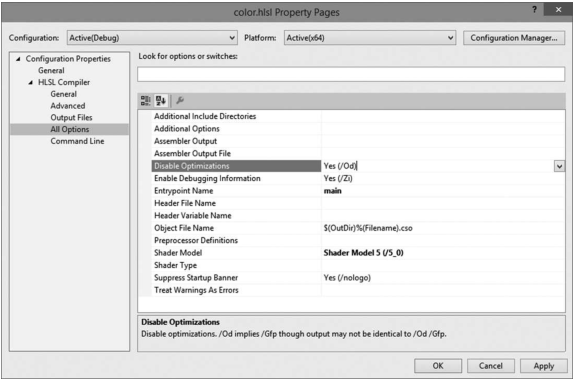
\includegraphics[width=\textwidth]{6-6}
    \centering
    \caption{添加一个自定义编译工具到项目中}
    \label{fig:6-6}
\end{figure}

使用VS集成HLSL支持的一个缺点是它只支持每个文件一个着色器程序。 因此,您不能将顶点和像素着色器存储在一个文件中。 此外,有时候我们希望使用不同的预处理器指令编译相同的着色器程序,以获得着色器的不同变体。 同样,这将不可能使用集成VS支持,因为它是每个.hlsl输入一个.cso输出。
\end{flushleft}

\section{光栅化器状态(Rasterizer State)}
\begin{flushleft}
虽然渲染管线的许多部分都是可编程的,但某些部分只能配置。 由D3D12\_RASTERIZER\_DESC结构表示的光栅化器状态组用于配置渲染管线的光栅化阶段:\\
\begin{lstlisting}
typedef struct D3D12_RASTERIZER_DESC
{
    D3D12_FILL_MODE FillMode;   // Default: D3D12_FILL_SOLID
    D3D12_CULL_MODE CullMode;   // Default: D3D12_CULL_BACK
    BOOL FrontCounterClockwise; // Default: false
    INT DepthBias;              // Default: 0
    FLOAT DepthBiasClamp;       // Default: 0.0f
    FLOAT SlopeScaledDepthBias; // Default: 0.0f
    BOOL DepthClipEnable;       // Default: true
    BOOL ScissorEnable;         // Default: false
    BOOL MultisampleEnable;     // Default: false
    BOOL AntialiasedLineEnable; // Default: false
    UINT ForcedSampleCount;     // Default: 0

    // Default: D3D12_CONSERVATIVE_RASTERIZATION_MODE_OFF
    D3D12_CONSERVATIVE_RASTERIZATION_MODE ConservativeRaster;
} D3D12_RASTERIZER_DESC;
\end{lstlisting}
这些成员大多数是高级选项或不经常使用;详细描述请参阅SDK文档。我们在这里只描述四个。\\
~\\
1.FillMode: 指定 D3D12\_FILL\_WIREFRAME 进行线框渲染或 D3D12\_FILL\_SOLID 用于实体渲染。固体渲染是默认的。\\
2.CullMode: 指定 D3D12\_CULL\_NONE 禁用剔除,D3D12\_CULL\_BACK 剔除背向三角形,或 D3D12\_CULL\_FRONT 剔除前向三角形。 背面三角形默认为剔除。\\
3.FrontCounterClockwise: 如果希望顺时针(相对于相机)顺时针排列的三角形被视为正面,并且逆时针(相对于相机)排列的三角形被视为背面,则指定false。 如果您希望将逆时针(相对于相机)排列的三角形视为正面,并将顺时针(相对于相机)排列的三角形视为背面,请指定true。 此状态默认为false。\\
4.ScissorEnable: 指定true以启用裁剪测试(第4.3.10节),如果为false则禁用它。 默认值是false。\\
~\\
以下代码表示如何创建打开线框模式并禁用背面剔除的栅格化状态:\\
\begin{lstlisting}
CD3DX12_RASTERIZER_DESC rsDesc(D3D12_DEFAULT);
rsDesc.FillMode = D3D12_FILL_WIREFRAME;
rsDesc.CullMode = D3D12_CULL_MODE;
\end{lstlisting}
CD3DX12\_RASTERIZER\_DESC 是一个便捷类,它扩展了 D3D12\_RASTERIZER\_DESC 并添加了一些辅助构造函数。 特别是,它有一个构造函数,它接受一个类型为 CD3D12\_DEFAULT 的对象,该对象只是一个用于重载的虚拟类型,用于将光栅化器状态成员初始化为默认值。CD3D12\_DEFAULT 和 D3D12\_DEFAULT 定义如下:\\
\begin{lstlisting}
struct CD3D12_DEFAULT {};
extern const DECLSPEC_SELECTANY CD3D12_DEFAULT D3D12_DEFAULT;
\end{lstlisting}
几个 Direct3D 便利类会使用 D3D12\_DEFAULT。
\end{flushleft}

\section{管道状态对象(Pipeline State Object)}
\begin{flushleft}
我们已经展示了如何描述输入布局描述,如何创建顶点和像素着色器,以及如何配置光栅器状态组。 但是,我们尚未显示如何将这些对象绑定到图形管道以供实际使用。 控制图形管道状态的大多数对象都被指定为一个称为管道状态对象(PSO)的聚合,它由 ID3D12PipelineState 接口表示。 为了创建一个PSO,我们首先通过填写一个D3D12\_GRAPHICS\_PIPELINE\_STATE\_DESC实例来描述它:\\
\end{flushleft}
\begin{lstlisting}
typedef struct D3D12_GRAPHICS_PIPELINE_STATE_DESC
{
    ID3D12RootSignature *pRootSignature;
    D3D12_SHADER_BYTECODE VS;
    D3D12_SHADER_BYTECODE PS;
    D3D12_SHADER_BYTECODE DS;
    D3D12_SHADER_BYTECODE HS;
    D3D12_SHADER_BYTECODE GS;
    D3D12_STREAM_OUTPUT_DESC StreamOutput;
    D3D12_BLEND_DESC BlendState;
    UINT SampleMask;
    D3D12_RASTERIZER_DESC RasterizerState;
    D3D12_DEPTH_STENCIL_DESC DepthStencilState;
    D3D12_INPUT_LAYOUT_DESC InputLayout;
    D3D12_PRIMITIVE_TOPOLOGY_TYPE PrimitiveTopologyType;
    UINT NumRenderTargets;
    DXGI_FORMAT RTVFormats[8];
    DXGI_FORMAT DSVFormat;
    DXGI_SAMPLE_DESC SampleDesc;
} D3D12_GRAPHICS_PIPELINE_STATE_DESC;
\end{lstlisting}
\begin{flushleft}
1.pRootSignature: 指向与此PSO绑定的根签名的指针。根签名必须与此PSO指定的着色器兼容。\\
2.VS: 要绑定的顶点着色器。 这由 D3D12\_SHADER\_BYTECODE 结构指定,该结构是指向编译的字节码数据的指针,以及字节码数据的大小(以字节为单位)。\\
3.PS: 要绑定的像素着色器。\\
4.DS: 要绑定的域着色器。(我们将在之后的章节讨论)\\
5.HS: 要绑定的外壳着色器。(我们将在之后的章节讨论)\\
6.GS: 要绑定的几何着色器。(我们将在之后的章节讨论)\\
7.StreamOutput: 用于称(流出)stream-out的高级技术。现在我们只是把这个领域归零(zero-out)。\\
8.BlendState: 指定配置混合的混合状态。 我们将在后面的章节中讨论这个状态组; 现在,指定默认 CD3DX12\_BLEND\_DESC(D3D12\_DEFAULT)。\\
9.SampleMask: 多重采样可能需要多达32个样本。 该32位整数值用于启用/禁用采样。 例如,如果关闭第5位,则第5个采样不会被采用。 当然,如果您实际使用至少5个采样的多重采样,则禁用第5个采样只会产生任何结果。 如果应用程序使用单个采样,则只有该参数的第一位很重要。 通常使用默认的0xffffffff,这不会禁用任何样本。\\
10.RasterizerState: 指定配置光栅化器的光栅化状态。\\
11.DepthStencilState: 指定配置深度/模板测试的深度/模板状态。 我们将在后面的章节中讨论这个状态组; 现在,指定默认CD3DX12\_DEPTH\_STENCIL\_DESC(D3D12\_DEFAULT)。
12.InputLayout: 输入布局描述,它只是D3D12\_INPUT\_ELEMENT\_DESC元素的一个数组,以及数组中的元素数。\\
\begin{lstlisting}
typedef struct D3D12_INPUT_LAYOUT_DESC
{
    const D3D12_INPUT_ELEMENT_DESC *pInputElementDescs;
    UINT NumElements;
} D3D12_INPUT_LAYOUT_DESC;
\end{lstlisting}
13.PrimitiveTopologyType: 指定原始拓扑类型。\\
\begin{lstlisting}
typedef enum D3D12_PRIMITIVE_TOPOLOGY_TYPE
{
    D3D12_PRIMITIVE_TOPOLOGY_TYPE_UNDEFINED = 0,
    D3D12_PRIMITIVE_TOPOLOGY_TYPE_POINT = 1,
    D3D12_PRIMITIVE_TOPOLOGY_TYPE_LINE = 2,
    D3D12_PRIMITIVE_TOPOLOGY_TYPE_TRIANGLE = 3,
    D3D12_PRIMITIVE_TOPOLOGY_TYPE_PATCH = 4
} D3D12_PRIMITIVE_TOPOLOGY_TYPE;
\end{lstlisting}
14.NumRenderTargets: 我们正在同时使用的渲染目标的数量。\\
15.RTVFormats: 呈现目标格式。 这是一个支持同时写入多个渲染目标的数组。 这应该与我们使用PSO的渲染目标的设置相匹配。\\
16.DSVFormat: 深度/模板缓冲区的格式。 这应该与我们使用PSO的深度/模板缓冲区的设置匹配。\\
17.SampleDesc: 介绍多重采样计数和质量级别。 这应该与我们正在使用的渲染目标的设置相匹配。\\
~\\
在我们填写完一个 D3D12\_GRAPHICS\_PIPELINE\_STATE\_DESC 实例后,我们使用 ID3D12Device::CreateGraphicsPipelineState 方法创建一个 ID3D12PipelineState 对象:\\
\begin{lstlisting}
ComPtr<ID3D12RootSignature> mRootSignature;
std::vector<D3D12_INPUT_ELEMENT_DESC> mInputLayout;
ComPtr<ID3DBlob> mvsByteCode;
ComPtr<ID3DBlob> mpsByteCode;
...
D3D12_GRAPHICS_PIPELINE_STATE_DESC psoDesc;
ZeroMemory(&psoDesc, 
           sizeof(D3D12_GRAPHICS_PIPELINE_STATE_DESC));
psoDesc.InputLayout = {
    mInputLayout.data(),
   (UINT)mInputLayout.size()
};
psoDesc.pRootSignature = mRootSignature.Get();
psoDesc.VS = {
    reinterpret_cast<BYTE*>(mvsByteCode->GetBufferPointer()),
    mvsByteCode->GetBufferSize()
};
psoDesc.PS = {
    reinterpret_cast<BYTE*>(mpsByteCode->GetBufferPointer()),
    mpsByteCode->GetBufferSize()
};
psoDesc.RasterizerState = CD3D12_RASTERIZER_DESC(D3D12_DEFAULT);
psoDesc.BlendState = CD3D12_BLEND_DESC(D3D12_DEFAULT);
psoDesc.DepthStencilState = CD3D12_DEPTH_STENCIL_DESC(D3D12_DEFAULT);
psoDesc.SampleMask = UINT_MAX;
psoDesc.PrimitiveTopologyType = D3D12_PRIMITIVE_TOPOLOGY_TYPE_TRIANGLE;
psoDesc.NumRenderTargets = 1;
psoDesc.RTVFormats[0] = mBackBufferFormat;
psoDesc.SampleDesc.Count = m4xMsaaState ? 4 : 1;
psoDesc.SampleDesc.Quality = m4xMsaaState ? (m4xMsaaQuality - 1) : 0;
psoDesc.DSVFormat = mDepthStencilFormat;

ComPtr<ID3D12PipelineState> mPSO;
md3dDevice->CreateGraphicsPipelineState(&psoDesc,IID_PPV_ARGS(&mPSO)));
\end{lstlisting}
上述代码用 ID3D12PipelineState 对象聚合(aggregate)了很多状态,出于性能考虑,我们指定所有这些对象都作为一个聚合传递到图形管线中。通过将它们作为聚合,Direct3D可以验证所有状态是否兼容,驱动程序可以预先生成所有代码以编写硬件状态。在Direct3D 11状态模型中,这些渲染状态片段是分开设置的。但是,各个状态是相关的; 如果一个状态被改变,它可能会另外要求驱动程序重新编程硬件以获取另一个依赖状态。由于配置流水线的许多状态会被改变,所以硬件的状态可能会被多次重新编写。为了避免这种情况,驱动程序通常推迟对硬件状态进行编写,直到在整个管道状态将被知道时发出绘制调用。但是这种延期需要驱动在运行时进行额外的记录工作; 它需要跟踪哪些状态发生了变化,然后生成代码以在运行时对硬件状态进行编程。 在新的Direct3D 12模型中,驱动程序可以在初始化时生成编程流水线状态所需的所有代码,因为我们将大部分流水线状态指定为聚合。\\
~\\
NOTICE:由于PSO验证和创建可能非常耗时,PSO应该在初始化时生成。 对此的一个例外可能是在运行时第一次引用PSO时创建PSO; 然后将其存储在哈希表等集合中,以便将来可以快速获取以供将来使用。\\
~\\
并非所有渲染状态都封装在PSO中。 一些像视口和裁剪矩形的状态是独立于PSO的。 这种状态可以独立于另一个管道状态而有效地设置,因此将它们包含在PSO中没有任何优势。\\
Direct3D基本上是一个状态机。 在我们改变它们之前,事物会保持现状。 如果您正在绘制的某些对象使用一个PSO,并且您正在绘制的其他对象需要不同的PSO,那么您需要像这样构造代码:\\
\begin{lstlisting}
// Reset specifies initial PSO.
mCommandList->Reset(mDirectCmdListAlloc.Get(), mPSO1.Get());
/*...draw objects using PSO 1...*/
// Change PSO
mCommandList->SetPipelineState(mPSO2.Get());
/*...draw objects using PSO 2...*/
// Change PSO
mCommandList->SetPipelineState(mPSO3.Get());
/*...draw objects using PSO 3...*/
\end{lstlisting}
换句话说,当PSO绑定到命令列表时,它不会改变,直到你覆盖它(或命令列表被重置)。\\
~\\
NOTICE: 出于性能考虑,PSO状态变化应该保持在最小。 一起绘制可以使用相同PSO的所有对象。 不要更改每次绘制调用的PSO!
\end{flushleft}

\section{几何工具结构体(Geometry Helper Structure)}
\begin{flushleft}
创建一个将顶点和索引缓冲区组合在一起以定义一组几何体的结构会很有帮助。 另外,这种结构可以保留顶点和索引数据的系统内存支持,以便可以由CPU读取。 CPU将需要访问几何数据以进行拾取和碰撞检测等操作。 另外,结构缓存顶点和索引缓冲区的重要属性,如格式和碰撞,并提供返回视图到缓冲区的方法。 每当我们定义一个几何体块时,我们在整本书中使用下面的MeshGeometry(在d3dUtil.h中定义)结构。\\
\begin{lstlisting}
// Defines a subrange of geometry in a MeshGeometry. This is for when
// multiple geometries are stored in one vertex and index buffer. It
// provides the offsets and data needed to draw a subset of geometry
// stores in the vertex and index buffers so that we can implement the
// technique described by Figure \ref{fig:6-3}.
struct SubmeshGeometry
{
    UINT IndexCount = 0;
    UINT StartIndexLocation = 0;
    INT  BaseVertexLocation = 0;

    // Bounding box of the geometry defined by this submesh.
    // This is used in later chapters of the book.
    DirectX::BoundingBox Bounds;
};

struct MeshGeometry
{
    // Give it a name so we can look it up by name.
    std::string Name;

    // System memory copies. Use Blobs because the vertex/index format can
    // be generic.
    // It is up to the client to cast appropriately.
    Microsoft::WRL::ComPtr<ID3DBlob> VertexBufferCPU = nullptr;
    Microsoft::WRL::ComPtr<ID3DBlob> IndexBufferCPU = nullptr;

    Microsoft::WRL::ComPtr<ID3D12Resource> VertexBufferGPU = nullptr;
    Microsoft::WRL::ComPtr<ID3D12Resource> IndexBufferGPU = nullptr;
    
    Microsoft::WRL::ComPtr<ID3D12Resource> VertexBufferUploader = nullptr;
    Microsoft::WRL::ComPtr<ID3D12Resource> IndexBufferUploader = nullptr;
    
    // Data about the buffers
    UINT VertexByteStride = 0;
    UINT VertexBufferByteSize = 0;
    DXGI_FORMAT IndexFormat = DXGI_FORMAT_R16_UINT;
    UINT IndexBufferByteSize = 0;
    
    // A MeshGeometry may store multiple geometries in one vertex/index
    // buffer.
    // Use this container to define the Submesh geometries so we can draw
    // the Submeshes individually.
    std::unordered_map<std::string, SubmeshGeometry> DrawArgs;
    
    D3D12_VERTEX_BUFFER_VIEW VertexBufferView() const
        D3D12_VERTEX_BUFFER_VIEW vbv;
    {
        vbv.BufferLocation = VertexBufferGPU->GetGPUVirtualAddress();
        vbv.StrideInBytes = VertexByteStride;
        vbv.SizeInBytes = VertexBufferByteSize;

        return vbv;
    }
    
    D3D12_INDEX_BUFFER_VIEW IndexBufferView() const
    {
        D3D12_INDEX_BUFFER_VIEW ibv;
        ibv.BufferLocation = IndexBufferGPU->GetGPUVirtualAddress();
        ibv.Format = IndexFormat;
        ibv.SizeInBytes = IndexBufferByteSize;

        return ibv;
    }
    
    // We can free this memory after we finish upload to the GPU.
    void DisposeUploaders()
    {
       VertexBufferUploader = nullptr;
       IndexBufferUploader = nullptr;
    }
};
\end{lstlisting}
\end{flushleft}

\section{BOX DEMO}
\begin{flushleft}
最后,我们已经有足够的能力去做出渲染一个彩箱(彩色立方体)的DEMO。这个例子基本上将我们在本章中讨论过的所有内容都放到了一个程序中。 读者应该研究代码并参考本章前面的部分,直到理解每一行。程序所使用的 Shaders\\color.hlsl, 见 6.5 节(像素着色器例子)末尾。
\end{flushleft}
\begin{lstlisting}
//**************************************************************************
// BoxApp.cpp by Frank Luna (C) 2015 All Rights Reserved.
//
// Shows how to draw a box in Direct3D 12.
//
// Controls:
//   Hold the left mouse button down and move the mouse to rotate.
//   Hold the right mouse button down and move the mouse to zoom in and out.
//**************************************************************************

#include "../../Common/d3dApp.h"
#include "../../Common/MathHelper.h"
#include "../../Common/UploadBuffer.h"

using Microsoft::WRL::ComPtr;
using namespace DirectX;
using namespace DirectX::PackedVector;

struct Vertex
{
    XMFLOAT3 Pos;
    XMFLOAT4 Color;
};

struct ObjectConstants
{
    XMFLOAT4X4 WorldViewProj = MathHelper::Identity4x4();
};

class BoxApp : public D3DApp
{
public:
    BoxApp(HINSTANCE hInstance);
    BoxApp(const BoxApp& rhs) = delete;
    BoxApp& operator=(const BoxApp& rhs) = delete;
    ~BoxApp();

    virtual bool Initialize()override;

private:
    virtual void OnResize()override;
    virtual void Update(const GameTimer& gt)override;
    virtual void Draw(const GameTimer& gt)override;

    virtual void OnMouseDown(WPARAM btnState, int x, int y)override;
    virtual void OnMouseUp(WPARAM btnState, int x, int y)override;
    virtual void OnMouseMove(WPARAM btnState, int x, int y)override;

    void BuildDescriptorHeaps();
    void BuildConstantBuffers();
    void BuildRootSignature();
    void BuildShadersAndInputLayout();
    void BuildBoxGeometry();
    void BuildPSO();

private:
    
    ComPtr<ID3D12RootSignature> mRootSignature = nullptr;
    ComPtr<ID3D12DescriptorHeap> mCbvHeap = nullptr;

    std::unique_ptr<UploadBuffer<ObjectConstants>> mObjectCB = nullptr;

    std::unique_ptr<MeshGeometry> mBoxGeo = nullptr;

    ComPtr<ID3DBlob> mvsByteCode = nullptr;
    ComPtr<ID3DBlob> mpsByteCode = nullptr;

    std::vector<D3D12_INPUT_ELEMENT_DESC> mInputLayout;

    ComPtr<ID3D12PipelineState> mPSO = nullptr;

    XMFLOAT4X4 mWorld = MathHelper::Identity4x4();
    XMFLOAT4X4 mView = MathHelper::Identity4x4();
    XMFLOAT4X4 mProj = MathHelper::Identity4x4();

    float mTheta = 1.5f*XM_PI;
    float mPhi = XM_PIDIV4;
    float mRadius = 5.0f;

    POINT mLastMousePos;
};

int WINAPI WinMain(HINSTANCE hInstance, HINSTANCE prevInstance,
                   PSTR cmdLine, int showCmd)
{
    // Enable run-time memory check for debug builds.
#if defined(DEBUG) | defined(_DEBUG)
    _CrtSetDbgFlag( _CRTDBG_ALLOC_MEM_DF | _CRTDBG_LEAK_CHECK_DF );
#endif

    try
    {
        BoxApp theApp(hInstance);
        if(!theApp.Initialize())
            return 0;

        return theApp.Run();
    }
    catch(DxException& e)
    {
        MessageBox(nullptr, e.ToString().c_str(), L"HR Failed", MB_OK);
        return 0;
    }
}

BoxApp::BoxApp(HINSTANCE hInstance)
: D3DApp(hInstance) 
{
}

BoxApp::~BoxApp()
{
}

bool BoxApp::Initialize()
{
    if(!D3DApp::Initialize())
        return false;
        
    // Reset the command list to prep for initialization commands.
    ThrowIfFailed(mCommandList->Reset(mDirectCmdListAlloc.Get(), nullptr));
 
    BuildDescriptorHeaps();
    BuildConstantBuffers();
    BuildRootSignature();
    BuildShadersAndInputLayout();
    BuildBoxGeometry();
    BuildPSO();

    // Execute the initialization commands.
    ThrowIfFailed(mCommandList->Close());
    ID3D12CommandList* cmdsLists[] = { mCommandList.Get() };
    mCommandQueue->ExecuteCommandLists(_countof(cmdsLists), cmdsLists);

    // Wait until initialization is complete.
    FlushCommandQueue();

    return true;
}

void BoxApp::OnResize()
{
    D3DApp::OnResize();

    // The window resized, so update the aspect ratio 
    // and recompute the projection matrix.
    XMMATRIX P = XMMatrixPerspectiveFovLH(
                     0.25f*MathHelper::Pi, 
                     AspectRatio(), 
                     1.0f, 1000.0f);
    XMStoreFloat4x4(&mProj, P);
}

void BoxApp::Update(const GameTimer& gt)
{
    // Convert Spherical to Cartesian coordinates.
    float x = mRadius*sinf(mPhi)*cosf(mTheta);
    float z = mRadius*sinf(mPhi)*sinf(mTheta);
    float y = mRadius*cosf(mPhi);

    // Build the view matrix.
    XMVECTOR pos = XMVectorSet(x, y, z, 1.0f);
    XMVECTOR target = XMVectorZero();
    XMVECTOR up = XMVectorSet(0.0f, 1.0f, 0.0f, 0.0f);

    XMMATRIX view = XMMatrixLookAtLH(pos, target, up);
    XMStoreFloat4x4(&mView, view);

    XMMATRIX world = XMLoadFloat4x4(&mWorld);
    XMMATRIX proj = XMLoadFloat4x4(&mProj);
    XMMATRIX worldViewProj = world*view*proj;

    // Update the constant buffer with 
    // the latest worldViewProj matrix.
    ObjectConstants objConstants;
    XMStoreFloat4x4(&objConstants.WorldViewProj, 
                    XMMatrixTranspose(worldViewProj));
    mObjectCB->CopyData(0, objConstants);
}

void BoxApp::Draw(const GameTimer& gt)
{
    // Reuse the memory associated with command recording.
    // We can only reset when the associated command lists 
    // have finished execution on the GPU.
    ThrowIfFailed(mDirectCmdListAlloc->Reset());

    // A command list can be reset after it has 
    // been added to the command queue via ExecuteCommandList.
    // Reusing the command list reuses memory.
    ThrowIfFailed(mCommandList->Reset(mDirectCmdListAlloc.Get(), 
                                      mPSO.Get()));

    mCommandList->RSSetViewports(1, &mScreenViewport);
    mCommandList->RSSetScissorRects(1, &mScissorRect);

    // Indicate a state transition on the resource usage.
    mCommandList->ResourceBarrier(1, 
                 &CD3DX12_RESOURCE_BARRIER::Transition(
                      CurrentBackBuffer(),
                      D3D12_RESOURCE_STATE_PRESENT, 
                      D3D12_RESOURCE_STATE_RENDER_TARGET));

    // Clear the back buffer and depth buffer.
    mCommandList->ClearRenderTargetView(
                      CurrentBackBufferView(), 
                      Colors::LightSteelBlue, 
                      0, nullptr);
    mCommandList->ClearDepthStencilView(
                      DepthStencilView(), 
                      D3D12_CLEAR_FLAG_DEPTH | D3D12_CLEAR_FLAG_STENCIL, 
                      1.0f, 0, 0, nullptr);
    
    // Specify the buffers we are going to render to.
    mCommandList->OMSetRenderTargets(1, 
                        &CurrentBackBufferView(), 
                        true, 
                        &DepthStencilView());

    ID3D12DescriptorHeap* descriptorHeaps[] = { mCbvHeap.Get() };
    mCommandList->SetDescriptorHeaps(_countof(descriptorHeaps), 
                                     descriptorHeaps);

    mCommandList->SetGraphicsRootSignature(mRootSignature.Get());

    mCommandList->IASetVertexBuffers(
                      0, 1, &mBoxGeo->VertexBufferView());
    mCommandList->IASetIndexBuffer(
                      &mBoxGeo->IndexBufferView());
    mCommandList->IASetPrimitiveTopology(
                      D3D11_PRIMITIVE_TOPOLOGY_TRIANGLELIST);
    
    mCommandList->SetGraphicsRootDescriptorTable(0, 
                      mCbvHeap->GetGPUDescriptorHandleForHeapStart());

    mCommandList->DrawIndexedInstanced(
        mBoxGeo->DrawArgs["box"].IndexCount, 
        1, 0, 0, 0);
    
    // Indicate a state transition on the resource usage.
    mCommandList->ResourceBarrier(1, 
                 &CD3DX12_RESOURCE_BARRIER::Transition(
                      CurrentBackBuffer(),
                      D3D12_RESOURCE_STATE_RENDER_TARGET, 
                      D3D12_RESOURCE_STATE_PRESENT));

    // Done recording commands.
    ThrowIfFailed(mCommandList->Close());
 
    // Add the command list to the queue for execution.
    ID3D12CommandList* cmdsLists[] = { mCommandList.Get() };
    mCommandQueue->ExecuteCommandLists(_countof(cmdsLists), cmdsLists);
    
    // swap the back and front buffers
    ThrowIfFailed(mSwapChain->Present(0, 0));
    mCurrBackBuffer = (mCurrBackBuffer + 1) % SwapChainBufferCount;

    // Wait until frame commands are complete.  
    // This waiting is inefficient and is
    // done for simplicity.  Later we will 
    // show how to organize our rendering code
    // so we do not have to wait per frame.
    FlushCommandQueue();
}

void BoxApp::OnMouseDown(WPARAM btnState, int x, int y)
{
    mLastMousePos.x = x;
    mLastMousePos.y = y;

    SetCapture(mhMainWnd);
}

void BoxApp::OnMouseUp(WPARAM btnState, int x, int y)
{
    ReleaseCapture();
}

void BoxApp::OnMouseMove(WPARAM btnState, int x, int y)
{
    if((btnState & MK_LBUTTON) != 0)
    {
        // Make each pixel correspond to a quarter of a degree.
        float dx = XMConvertToRadians(
                       0.25f*static_cast<float>(x - mLastMousePos.x));
        float dy = XMConvertToRadians(
                       0.25f*static_cast<float>(y - mLastMousePos.y));

        // Update angles based on input to orbit camera around box.
        mTheta += dx;
        mPhi += dy;

        // Restrict the angle mPhi.
        mPhi = MathHelper::Clamp(mPhi, 0.1f, MathHelper::Pi - 0.1f);
    }
    else if((btnState & MK_RBUTTON) != 0)
    {
        // Make each pixel correspond to 0.005 unit in the scene.
        float dx = 0.005f*static_cast<float>(x - mLastMousePos.x);
        float dy = 0.005f*static_cast<float>(y - mLastMousePos.y);

        // Update the camera radius based on input.
        mRadius += dx - dy;

        // Restrict the radius.
        mRadius = MathHelper::Clamp(mRadius, 3.0f, 15.0f);
    }

    mLastMousePos.x = x;
    mLastMousePos.y = y;
}

void BoxApp::BuildDescriptorHeaps()
{
    D3D12_DESCRIPTOR_HEAP_DESC cbvHeapDesc;
    cbvHeapDesc.NumDescriptors = 1;
    cbvHeapDesc.Type = D3D12_DESCRIPTOR_HEAP_TYPE_CBV_SRV_UAV;
    cbvHeapDesc.Flags = D3D12_DESCRIPTOR_HEAP_FLAG_SHADER_VISIBLE;
    cbvHeapDesc.NodeMask = 0;
    ThrowIfFailed(md3dDevice->CreateDescriptorHeap(&cbvHeapDesc,
        IID_PPV_ARGS(&mCbvHeap)));
}

void BoxApp::BuildConstantBuffers()
{
    mObjectCB = std::make_unique<UploadBuffer<ObjectConstants>>(
                    md3dDevice.Get(), 1, true);

    UINT objCBByteSize = d3dUtil::CalcConstantBufferByteSize(
                             sizeof(ObjectConstants));

    D3D12_GPU_VIRTUAL_ADDRESS cbAddress = mObjectCB->Resource()
                                              ->GetGPUVirtualAddress();

    // Offset to the ith object constant buffer in the buffer.
    int boxCBufIndex = 0;
    cbAddress += boxCBufIndex*objCBByteSize;

    D3D12_CONSTANT_BUFFER_VIEW_DESC cbvDesc;
    cbvDesc.BufferLocation = cbAddress;
    cbvDesc.SizeInBytes = d3dUtil::CalcConstantBufferByteSize(
                              sizeof(ObjectConstants));

    md3dDevice->CreateConstantBufferView(
        &cbvDesc,
        mCbvHeap->GetCPUDescriptorHandleForHeapStart());
}

void BoxApp::BuildRootSignature()
{
    // Shader programs typically require resources as input 
    // (constant buffers, textures, samplers).  
    // The root signature defines the resources the shader
    // programs expect.  If we think of the shader programs 
    // as a function, and the input resources as function parameters,
    // then the root signature can be thought of as defining
    // the function signature.  

    // Root parameter can be a table, root descriptor or root constants.
    CD3DX12_ROOT_PARAMETER slotRootParameter[1];

    // Create a single descriptor table of CBVs.
    CD3DX12_DESCRIPTOR_RANGE cbvTable;
    cbvTable.Init(D3D12_DESCRIPTOR_RANGE_TYPE_CBV, 1, 0);
    slotRootParameter[0].InitAsDescriptorTable(1, &cbvTable);

    // A root signature is an array of root parameters.
    CD3DX12_ROOT_SIGNATURE_DESC rootSigDesc(1, slotRootParameter, 
                                            0, nullptr, 
        D3D12_ROOT_SIGNATURE_FLAG_ALLOW_INPUT_ASSEMBLER_INPUT_LAYOUT);

    // create a root signature with a single slot
    // which points to a descriptor range consisting 
    // of a single constant buffer
    ComPtr<ID3DBlob> serializedRootSig = nullptr;
    ComPtr<ID3DBlob> errorBlob = nullptr;
    HRESULT hr = D3D12SerializeRootSignature(&rootSigDesc, 
                     D3D_ROOT_SIGNATURE_VERSION_1,
                     serializedRootSig.GetAddressOf(), 
                     errorBlob.GetAddressOf());

    if(errorBlob != nullptr)
    {
        ::OutputDebugStringA((char*)errorBlob->GetBufferPointer());
    }
    ThrowIfFailed(hr);

    ThrowIfFailed(md3dDevice->CreateRootSignature(
        0,
        serializedRootSig->GetBufferPointer(),
        serializedRootSig->GetBufferSize(),
        IID_PPV_ARGS(&mRootSignature)));
}

void BoxApp::BuildShadersAndInputLayout()
{
    HRESULT hr = S_OK;
    
    mvsByteCode = d3dUtil::CompileShader(L"Shaders\\color.hlsl", 
                      nullptr, "VS", "vs_5_0");
    mpsByteCode = d3dUtil::CompileShader(L"Shaders\\color.hlsl", 
                      nullptr, "PS", "ps_5_0");

    mInputLayout =
    {
        { "POSITION", 0, DXGI_FORMAT_R32G32B32_FLOAT, 0, 0, 
                      D3D12_INPUT_CLASSIFICATION_PER_VERTEX_DATA, 0 },
        { "COLOR",    0, DXGI_FORMAT_R32G32B32A32_FLOAT, 0, 12, 
                      D3D12_INPUT_CLASSIFICATION_PER_VERTEX_DATA, 0 }
    };
}

void BoxApp::BuildBoxGeometry()
{
    std::array<Vertex, 8> vertices =
    {
        Vertex({ XMFLOAT3(-1.0f, -1.0f, -1.0f), XMFLOAT4(Colors::White) }),
        Vertex({ XMFLOAT3(-1.0f, +1.0f, -1.0f), XMFLOAT4(Colors::Black) }),
        Vertex({ XMFLOAT3(+1.0f, +1.0f, -1.0f), XMFLOAT4(Colors::Red) }),
        Vertex({ XMFLOAT3(+1.0f, -1.0f, -1.0f), XMFLOAT4(Colors::Green) }),
        Vertex({ XMFLOAT3(-1.0f, -1.0f, +1.0f), XMFLOAT4(Colors::Blue) }),
        Vertex({ XMFLOAT3(-1.0f, +1.0f, +1.0f), XMFLOAT4(Colors::Yellow) }),
        Vertex({ XMFLOAT3(+1.0f, +1.0f, +1.0f), XMFLOAT4(Colors::Cyan) }),
        Vertex({ XMFLOAT3(+1.0f, -1.0f, +1.0f), XMFLOAT4(Colors::Magenta) })
    };

    std::array<std::uint16_t, 36> indices =
    {
        // front face
        0, 1, 2,
        0, 2, 3,

        // back face
        4, 6, 5,
        4, 7, 6,

        // left face
        4, 5, 1,
        4, 1, 0,

        // right face
        3, 2, 6,
        3, 6, 7,

        // top face
        1, 5, 6,
        1, 6, 2,

        // bottom face
        4, 0, 3,
        4, 3, 7
    };

    const UINT vbByteSize = (UINT)vertices.size() * sizeof(Vertex);
    const UINT ibByteSize = (UINT)indices.size() * sizeof(std::uint16_t);

    mBoxGeo = std::make_unique<MeshGeometry>();
    mBoxGeo->Name = "boxGeo";

    ThrowIfFailed(D3DCreateBlob(vbByteSize, 
                                &mBoxGeo->VertexBufferCPU));
    CopyMemory(mBoxGeo->VertexBufferCPU->GetBufferPointer(),
               vertices.data(), vbByteSize);

    ThrowIfFailed(D3DCreateBlob(ibByteSize, 
                                &mBoxGeo->IndexBufferCPU));
    CopyMemory(mBoxGeo->IndexBufferCPU->GetBufferPointer(), 
               indices.data(), ibByteSize);

    mBoxGeo->VertexBufferGPU = d3dUtil::CreateDefaultBuffer(
                                   md3dDevice.Get(),
                                   mCommandList.Get(), 
                                   vertices.data(), 
                                   vbByteSize, 
                                   mBoxGeo->VertexBufferUploader);

    mBoxGeo->IndexBufferGPU = d3dUtil::CreateDefaultBuffer(
                                  md3dDevice.Get(),
                                  mCommandList.Get(),
                                  indices.data(), 
                                  ibByteSize, 
                                  mBoxGeo->IndexBufferUploader);

    mBoxGeo->VertexByteStride = sizeof(Vertex);
    mBoxGeo->VertexBufferByteSize = vbByteSize;
    mBoxGeo->IndexFormat = DXGI_FORMAT_R16_UINT;
    mBoxGeo->IndexBufferByteSize = ibByteSize;

    SubmeshGeometry submesh;
    submesh.IndexCount = (UINT)indices.size();
    submesh.StartIndexLocation = 0;
    submesh.BaseVertexLocation = 0;

    mBoxGeo->DrawArgs["box"] = submesh;
}

void BoxApp::BuildPSO()
{
    D3D12_GRAPHICS_PIPELINE_STATE_DESC psoDesc;
    ZeroMemory(&psoDesc, sizeof(D3D12_GRAPHICS_PIPELINE_STATE_DESC));
    psoDesc.InputLayout = { mInputLayout.data(), 
                            (UINT)mInputLayout.size() };
    psoDesc.pRootSignature = mRootSignature.Get();
    psoDesc.VS = 
    { 
        reinterpret_cast<BYTE*>(mvsByteCode->GetBufferPointer()), 
        mvsByteCode->GetBufferSize() 
    };
    psoDesc.PS = 
    { 
        reinterpret_cast<BYTE*>(mpsByteCode->GetBufferPointer()), 
        mpsByteCode->GetBufferSize() 
    };
    psoDesc.RasterizerState = CD3DX12_RASTERIZER_DESC(D3D12_DEFAULT);
    psoDesc.BlendState = CD3DX12_BLEND_DESC(D3D12_DEFAULT);
    psoDesc.DepthStencilState = CD3DX12_DEPTH_STENCIL_DESC(D3D12_DEFAULT);
    psoDesc.SampleMask = UINT_MAX;
    psoDesc.PrimitiveTopologyType = D3D12_PRIMITIVE_TOPOLOGY_TYPE_TRIANGLE;
    psoDesc.NumRenderTargets = 1;
    psoDesc.RTVFormats[0] = mBackBufferFormat;
    psoDesc.SampleDesc.Count = m4xMsaaState ? 4 : 1;
    psoDesc.SampleDesc.Quality = m4xMsaaState ? (m4xMsaaQuality - 1) : 0;
    psoDesc.DSVFormat = mDepthStencilFormat;
    ThrowIfFailed(md3dDevice->CreateGraphicsPipelineState(&psoDesc, 
                                   IID_PPV_ARGS(&mPSO)));
}
\end{lstlisting}
\begin{figure}[h]
	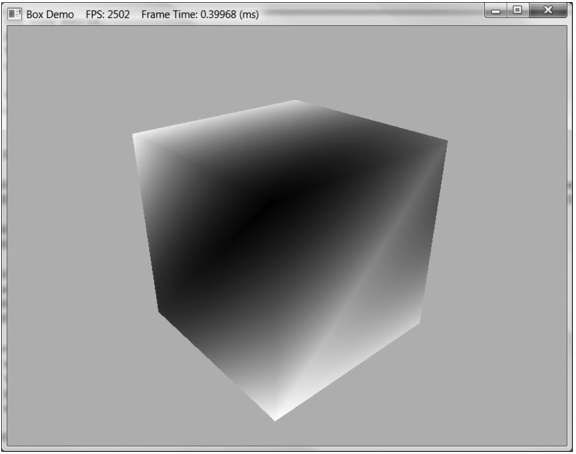
\includegraphics[width=\textwidth]{6-7}
	\centering
	\caption{Box DEMO 截图}
	\label{fig:6-7}
\end{figure}

\section{总结}
TODO:

\section{练习}
%---------- 1 ----------------
\begin{flushleft}
1. 写出下面顶点结构的 D3D12\_INPUT\_ELEMENT\_DESC 数组:
\end{flushleft}
\begin{lstlisting}
struct Vertex
{
    XMFLOAT3 Pos;
    XMFLOAT3 Tangent;
    XMFLOAT3 Normal;
    XMFLOAT2 Tex0;
    XMFLOAT2 Tex1;
    XMCOLOR  Color;
};
\end{lstlisting}

%---------- 2 ----------------
\begin{flushleft}
~\\
2. 重写彩箱DEMO,这次使用 2 个顶点缓冲区(2个输入槽)给管道提供顶点数据。一个缓冲区存储位置元素,另一个存储存储颜色元素。下面给定两个分开的顶点数据结构:\\
\end{flushleft}
\begin{lstlisting}
struct VPosData
{
    XMFLOAT3 Pos;
};

struct VColorData
{
    XMFLOAT4 Color;
};
\end{lstlisting}
\begin{flushleft}
位置元素挂在输入槽0上,颜色元素挂在输入操1上。此外还需注意 D3D12\_INPUT\_ELEMENT\_DESC::AlignedByteOffset 对于两个元素来说都是0;然后使用 ID3D12CommandList::IASetVertexBuffers 方法来将缓冲区绑定到槽0和槽1。然后,Direct3D将使用来自不同输入槽的元素来组合顶点。 这可以用作优化。 例如,在阴影映射算法中,我们需要每帧绘制两次场景:一次从光源的角度(阴影传递),一次从主摄像头的角度(主传递)。 阴影传递仅需要位置数据和纹理坐标(对于经过alpha测试的几何体)。 因此我们可以将顶点数据分成两个槽:一个槽包含位置和纹理坐标,另一个槽包含其他顶点属性(例如,法线和切线矢量)。 现在我们可以轻松地仅在阴影传递所需的顶点数据中流动(位置和纹理坐标),从而为阴影传递节省数据带宽。 主渲染过程将使用两个顶点输入槽来获取所需的所有顶点数据。 为了提高性能,建议最小化用于小于或等于3的小数字的输入槽数。\\
\end{flushleft}

%---------- 3 ----------------
\begin{flushleft}
3. 绘制以下图形:\\
\begin{itemize}
  \item 1. 一个点列表,如图5.13a。
  \item 2. 一个线段条,如图5.13b。
  \item 3. 一个线段列表,如图5.13c。
  \item 4. 一个三角条,如图5.13d。
  \item 5. 一个三角列表,如图5.14a。
\end{itemize}
\end{flushleft}

%---------- 4 ----------------
\begin{flushleft}
4. 构造金字塔的顶点和索引列表,如图\ref{fig:6-8}所示,并绘制它。 将基顶点设为绿色和顶上顶点设为红色。\\
\end{flushleft}
\begin{figure}[h]
    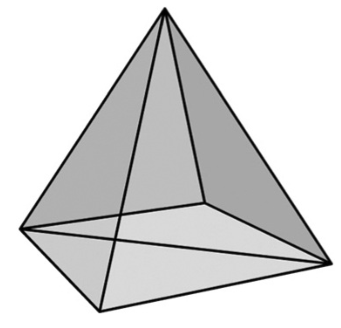
\includegraphics[width=\textwidth]{6-8}
    \centering
    \caption{金字塔三角形}
    \label{fig:6-8}
\end{figure}
%---------- 5 ----------------
\begin{flushleft}
5. 运行“Box” DEMO,并回想一下我们仅在顶点指定颜色。 解释如何为三角形上的每个像素获取像素颜色。
\end{flushleft}


%---------- 6 ----------------
\begin{flushleft}
6. 修改 Box Demo, 在转换为世界空间之前将以下变换应用于顶点着色器中的每个顶点。
\end{flushleft}
\begin{lstlisting}
vin.PosL.xy += 0.5f*sin(vinL.Pos.x)*sin(3.0f*gTime);
vin.PosL.z *= 0.6f + 0.4f*sin(2.0f*gTime);
\end{lstlisting}
\begin{flushleft}
您需要添加一个gTime常量缓冲区变量; 此变量对应于当前的 GameTimer::TotalTime() 值。 使用正弦函数周期性地扭曲顶点来将时间通过顶点动画来展现。
\end{flushleft}

%---------- 7 ----------------
\begin{flushleft}
7. 将箱(box)和金字塔的顶点(练习4)合并到一个大的顶点缓冲区中。 还将框和金字塔的索引合并到一个大索引缓冲区中(但不更新索引值)。 然后使用 ID3D12CommandList::DrawIndexedInstanced 的参数逐个绘制框和金字塔。 使用世界变换矩阵,使框和金字塔在世界空间中不相交。
\end{flushleft}

%---------- 8 ----------------
\begin{flushleft}
8. 通过在线框(wireframe)模式下渲染多维数据集来修改Box演示。
\end{flushleft}

%---------- 9 ----------------
\begin{flushleft}
9. 修改Box演示, 禁用背面剔除(D3D12\_CULL\_NONE); 也尝试剔除正面而不是背面(D3D12\_CULL\_FRONT)。 以线框(wireframe)模式输出结果,以便您可以更轻松地查看差异。
\end{flushleft}

%---------- 10 ----------------
\begin{flushleft}
10. 如果顶点内存很重要,那么从128位颜色值减少到32位颜色值可能是值得的。修改“Box”演示 在顶点结构中使用32位颜色值而不是128位颜色值。 您的顶点结构和相应的顶点输入描述将如下所示:\\
\end{flushleft}
\begin{lstlisting}
struct Vertex
{
    XMFLOAT3 Pos;
    XMCOLOR Color;
}

D3D12_INPUT_ELEMENT_DESC vertexDesc[] = {
    {“POSITION”, 0, DXGI_FORMAT_R32G32B32_FLOAT, 0, 0, 
                 D3D12_INPUT_PER_VERTEX_DATA, 0},
    {“COLOR”,    0, DXGI_FORMAT_B8G8R8A8_UNORM, 0, 12,
                 D3D12_INPUT_PER_VERTEX_DATA, 0}
};
\end{lstlisting}
\begin{flushleft}
我们使用 DXGI\_FORMAT\_B8G8R8A8\_UNORM 格式(8位红色,绿色,蓝色和alpha)。 此格式对应于常见的32位图形颜色格式ARGB,但 DXGI\_FORMAT 符号以小端表示法列出它们在内存中出现的字节。 在little-endian中,多字节(multi-byte)数据字(word)的字节从最低有效字节写入最高有效字节,这就是为什么 ARGB 在内存中出现为 BGRA,其中最小内存地址处的最低有效字节和最高有效字节为 最高的内存地址。
\end{flushleft}

%---------- 11 ----------------
\begin{flushleft}
11. 思考下面 C++ 顶点结构:
\end{flushleft}
\begin{lstlisting}
struct Vertex
{
    XMFLOAT3 Pos;
    XMFLOAT4 Color;
};
\end{lstlisting}
\begin{itemize}
  \item 1. 输入布局描述顺序是否需要匹配顶点结构顺序? 也就是说,以下顶点声明是否适用于此顶点结构? 做一个实验来找出答案。 然后给出你为什么认为它有效或无效的推理。
  \begin{lstlisting}
  D3D11_INPUT_ELEMENT_DESC vertexDesc[] =
  {
      {“COLOR”,    0, DXGI_FORMAT_R32G32B32A32_FLOAT, 0, 12,
                   D3D11_INPUT_PER_VERTEX_DATA, 0},
      {“POSITION”, 0, DXGI_FORMAT_R32G32B32_FLOAT, 0, 0,
                   D3D11_INPUT_PER_VERTEX_DATA, 0}
  };
  \end{lstlisting}
  \item 2. 相应的顶点着色器结构顺序是否需要匹配 C++ 顶点结构顺序? 也就是说,以下顶点着色器结构是否与上述 C++ 顶点结构一起使用? 做一个实验来找出答案。 然后给出你为什么认为它有效或无效的推理。
  \begin{lstlisting}
  struct VertexIn
  {
      float4 Color : COLOR;
      float3 Pos   : POSITION;
  };
  \end{lstlisting}
\end{itemize}

%---------- 12 ----------------
\begin{flushleft}
12. 将视口(viewport)设置为后缓冲区(back buffer)的左半部分。
\end{flushleft}

%---------- 13 ----------------
\begin{flushleft}
13. 使用剪刀测试来剔除以后缓冲区为中心的矩形外的所有像素,宽度为mClientWidth/2,高度为 mClientHeight/2。 请记住,您还需要使用光栅化器状态组启用剪刀测试。
\end{flushleft}

%---------- 14 ----------------
\begin{flushleft}
14. 像素着色器颜色色调。 使用常量缓冲区为颜色随时间变化。 使用平滑缓动功能。 在顶点着色器和像素着色器中执行此操作。
\end{flushleft}

%---------- 15 ----------------
\begin{flushleft}
15. 修改 Box DEMO 中的像素着色器为如下形式:
\end{flushleft}
\begin{lstlisting}
float4 PS(VertexOut pin) : SV_Target
{
    clip(pin.Color.r - 0.5f);
    return pin.Color;
}
\end{lstlisting}
\begin{flushleft}
运行程序并猜测内置 clip 方法的作用。
\end{flushleft}

%---------- 16 ----------------
\begin{flushleft}
修改 Box 演示中的像素着色器,以在插值顶点颜色和通过常量缓冲区指定的 gPulseColor 之间平滑脉冲。 您还需要更新应用程序端的常量缓冲区。 HLSL代码中的常量缓冲区和像素着色器应如下所示:
\end{flushleft}
\begin{lstlisting}
cbuffer cbPerObject : register(b0)
{
    float4x4 gWorldViewProj;
    float4 gPulseColor;
    float gTime;
};

float4 PS(VertexOut pin) : SV_Target
{
    const float pi = 3.14159;

    // Oscillate a value in [0,1] over time using a sine functio.
    float s = 0.5f*sin(2*gTime - 0.25f(pi) + 0.5f;

    // Linearly interpolate between pin.Color and gPulseColor based on
    // parameter s.
    float4 c = lerp(pin.Color, gPulseColor, s);
    return c;
}
\end{lstlisting}
\begin{flushleft}
gTime 变量对应于 GameTimer::TotalTime() 的值。
\end{flushleft}

\chapter{在Direct3D中绘制2(Drawing in Direct3D Part 2)}
\begin{flushleft}
本章介绍我们将在本书其余部分使用的一些绘图模式。 本章首先介绍一种绘图优化的方法,我们将其称为“帧资源”。使用帧资源,我们修改渲染循环,这样我们就不必每帧刷新命令队列; 这提高了CPU和GPU的利用率。 接下来,我们介绍渲染项的概念,并解释我们如何根据更新频率划分常量数据。 此外,我们更详细地检查根签名,并了解其他根参数类型:根描述符和根常量。 最后,我们展示了如何绘制一些更复杂的对象; 到本章结束时,您将能够绘制类似丘陵和山谷,圆柱体,球体和动画波浪模拟的表面。\\
~\\
{\large Objectives:}
\begin{itemize}
    \item 了解对渲染过程的修改,不要求我们每帧刷新命令队列,从而提高性能。
    \item 了解其他两种类型的根签名参数类型:根描述符和根常量。
    \item 探索如何在程序上生成和绘制常见的几何形状,如网格,圆柱体和球体。
    \item 了解我们如何在CPU上设置顶点动画并使用动态顶点缓冲区将新顶点位置上传到GPU。
\end{itemize}
\end{flushleft}

%---- 7.1 ------
\section{帧资源(Frame Resources)}
\begin{flushleft}
回忆 4.2 节,CPU和GPU并行工作。 CPU构建并提交命令列表(除了其他CPU工作之外),GPU处理命令队列中的命令。 目标是让CPU和GPU忙碌,以充分利用系统上可用的硬件资源。 到目前为止,在我们的演示中,我们已经每帧同步CPU和GPU一次。 两个例子解释这种同步的必要性:\\
\begin{itemize}
    \item 1.在GPU完成执行命令之前,不能重置命令分配器(command allocator)。 假设我们没有进行同步,以便CPU在GPU处理完当前帧n之前可以继续下一帧n + 1:如果CPU在帧n + 1中重置命令分配器,但GPU仍在处理命令 从第n帧开始,我们将清除GPU仍在使用的命令。
    \item 2.在GPU完成执行引用常量缓冲区的绘图命令之前,CPU无法更新常量缓冲区。 此示例对应于4.2.2节和图4.7中描述的情况。 假设我们没有进行同步,以便CPU在GPU完成处理当前帧n之前可以继续下一帧n + 1:如果CPU在帧n + 1中覆盖常量缓冲区数据,但GPU还没有 执行引用帧n中的常量缓冲区的绘制调用,然后常量缓冲区包含当GPU执行帧n的绘制调用时的错误数据。
\end{itemize}
因此,我们一直在每帧结束时调用 D3DApp::FlushCommandQueue,以确保GPU已完成执行帧的所有命令。 此解决方案有效,但由于以下原因效率低下:\\
\begin{itemize}
    \item 1.在帧开始时,GPU将不会有任何要处理的命令,因为我们等待清空命令队列。 它必须等到CPU构建并提交一些命令才能执行。
    \item 2.在帧结束时,CPU正在等待GPU完成处理命令。
\end{itemize}
所以每一帧,CPU和GPU都会在某些时候空闲。\\
~\\
该问题的一个解决方案是创建CPU修改每个帧所需的资源的循环数组。 我们称这种资源为帧资源,我们通常使用三个帧资源元素的循环数组。 对于帧n,CPU将循环通过帧资源队列以获得下一个可用(即,未被GPU使用)帧资源。 然后,CPU将执行任何资源更新,并在GPU处理先前帧时构建和提交帧n的命令列表。 然后CPU继续进行第n + 1帧并重复。 如果帧资源阵列有三个元素,这可以使CPU在GPU之前达到两帧,从而确保GPU保持忙碌状态。 下面是我们在本章中用于“Shapes”演示的帧资源类的示例。 由于CPU只需要在此演示中修改常量缓冲区,因此帧资源类仅包含常量缓冲区。\\
\end{flushleft}
\begin{lstlisting}
// Stores the resources needed for the CPU to build
// the command lists
// for a frame. The contents here will vary from app
// to app based on
// the needed resources.
struct FrameResource
{
public:
    FrameResource(ID3D12Device* device, UINT passCount, UINT objectCount);
    FrameResource(const FrameResource& rhs) = delete;
    FrameResource& operator=(const FrameResource& rhs) = delete;
    ~FrameResource();
    // We cannot reset the allocator until the GPU is
    // done processing the
    // commands. So each frame needs their own
    // allocator.
    Microsoft::WRL::ComPtr<ID3D12CommandAllocator> CmdListAlloc;
    
    // We cannot update a cbuffer until the GPU is done
    // processing the
    // commands that reference it. So each frame needs
    // their own cbuffers.
    std::unique_ptr<UploadBuffer<PassConstants>> PassCB = nullptr;
    std::unique_ptr<UploadBuffer<ObjectConstants>>
    ObjectCB = nullptr;
    // Fence value to mark commands up to this fence
    // point. This lets us
    // check if these frame resources are still in use
    // by the GPU.
    UINT64 Fence = 0;
};

FrameResource::FrameResource(ID3D12Device* device,
                             UINT passCount, UINT
                             objectCount)
{
    ThrowIfFailed(device->CreateCommandAllocator(
        D3D12_COMMAND_LIST_TYPE_DIRECT,
        IID_PPV_ARGS(CmdListAlloc.GetAddressOf())));
    PassCB = std::make_unique<UploadBuffer<PassConstants>>(
        device,
        passCount, 
        true);
    ObjectCB = std::make_unique<UploadBuffer<ObjectConstants>>(
        device,
        objectCount, true);
}
FrameResource::˜FrameResource() {}
\end{lstlisting}
\begin{flushleft}
然后,我们的应用程序类将三个帧资源的向量实例化,并设置成员变量以跟踪当前帧资源:\\
\end{flushleft}
\begin{lstlisting}
static const int NumFrameResources = 3;
std::vector<std::unique_ptr<FrameResource>> mFrameResources;
FrameResource* mCurrFrameResource = nullptr;
int mCurrFrameResourceIndex = 0;
void ShapesApp::BuildFrameResources()
{
    for(int i = 0; i < gNumFrameResources; ++i)
    {
        mFrameResources.push_back(std::make_unique<FrameResource>(
                                      md3dDevice.Get(), 
                                      1, 
                                      (UINT)mAllRitems.size()));
    }
}
\end{lstlisting}
\begin{flushleft}
现在,对于CPU帧n,算法的工作原理如下:\\
\end{flushleft}
\begin{lstlisting}
void ShapesApp::Update(const GameTimer& gt)
{
    // Cycle through the circular frame resource array.
    mCurrFrameResourceIndex = (mCurrFrameResourceIndex + 1) % NumFrameResources;
    mCurrFrameResource = mFrameResources[mCurrFrameResourceIndex];
    // Has the GPU finished processing the commands of
    // the current frame
    // resource. If not, wait until the GPU has
    // completed commands up to
    // this fence point.
    if(mCurrFrameResource->Fence != 0 &&
       mCommandQueue->GetLastCompletedFence() < mCurrFrameResource->Fence)
    {
        HANDLE eventHandle = CreateEventEx(nullptr, false, 
                                  false, EVENT_ALL_ACCESS);
        ThrowIfFailed(mCommandQueue->SetEventOnFenceCompletion(
             mCurrFrameResource->Fence, eventHandle));
        WaitForSingleObject(eventHandle, INFINITE);
        CloseHandle(eventHandle);
    }
    // […] Update resources in mCurrFrameResource (like cbuffers).
}
void ShapesApp::Draw(const GameTimer& gt)
{
    // […] Build and submit command lists for this frame.
    // Advance the fence value to mark commands up to
    // this fence point.
    mCurrFrameResource->Fence = ++mCurrentFence;
    // Add an instruction to the command queue to set a
    // new fence point.
    // Because we are on the GPU timeline, the new fence
    // point won’t be
    // set until the GPU finishes processing all the
    // commands prior to
    // this Signal().
    mCommandQueue->Signal(mFence.Get(), mCurrentFence);
    // Note that GPU could still be working on commands
    // from previous
    // frames, but that is okay, because we are not
    // touching any frame
    // resources associated with those frames.
}
\end{lstlisting}
\begin{flushleft}
请注意,此解决方案不会阻止等待。 如果一个处理器处理帧的速度比另一个处理器快得多,那么一个处理器最终将不得不等待另一个处理器赶上,因为我们不能让一个处理器远远超过另一个处理器。 如果GPU处理命令的速度比CPU提交工作的速度快,那么GPU将处于空闲状态。 一般来说,如果我们试图推动图形限制,我们希望避免这种情况,因为我们没有充分利用GPU。 另一方面,如果CPU总是以比GPU更快的速度处理帧,那么CPU将不得不在某个时刻等待。 这是理想的情况,因为GPU正在被充分利用; 额外的CPU周期总是可以用于游戏的其他部分,如AI,物理和游戏逻辑。\\
因此,如果多个帧资源不能阻止任何等待,它对我们有何帮助? 它可以帮助我们保持GPU的供给。 当GPU正在处理来自帧n的命令时,它允许CPU继续构建和提交帧n + 1和n + 2的命令。 这有助于保持命令队列非空,以便GPU始终有工作要做。
\end{flushleft}

%---- 7.2 ------
\section{渲染项(Render Items)}
\begin{flushleft}
绘制对象需要设置多个参数,例如绑定顶点和索引缓冲区,绑定对象常量,设置基本类型(primitive type)以及指定DrawIndexedInstanced参数。 当我们开始在场景中绘制更多对象时,创建一个存储绘制对象所需数据的轻量级结构会很有帮助。 这些数据因应用程序而异,因为我们添加了需要不同绘图数据的新功能。 我们将提交完整绘制所需的数据集称为渲染管道渲染项。 对于此演示,我们的RenderItem结构如下所示:\\
\end{flushleft}
\begin{lstlisting}
// Lightweight structure stores parameters to draw a shape.  This will
// vary from app-to-app.
struct RenderItem
{
    RenderItem() = default;

    // World matrix of the shape that describes the object's local space
    // relative to the world space, which defines the position, orientation,
    // and scale of the object in the world.
    XMFLOAT4X4 World = MathHelper::Identity4x4();

    // Dirty flag indicating the object data has changed 
    // and we need to update the constant buffer.
    // Because we have an object cbuffer for each FrameResource, 
    // we have to apply the update to each FrameResource.  
    // Thus, when we modify obect data we should set 
    // NumFramesDirty = gNumFrameResources so that each 
    // frame resource gets the update.
    int NumFramesDirty = gNumFrameResources;

    // Index into GPU constant buffer corresponding to 
    // the ObjectCB for this render item.
    UINT ObjCBIndex = -1;

    MeshGeometry* Geo = nullptr;

    // Primitive topology.
    D3D12_PRIMITIVE_TOPOLOGY PrimitiveType = D3D_PRIMITIVE_TOPOLOGY_TRIANGLELIST;

    // DrawIndexedInstanced parameters.
    UINT IndexCount = 0;
    UINT StartIndexLocation = 0;
    int BaseVertexLocation = 0;
};
\end{lstlisting}
\begin{flushleft}
我们的应用程序将根据需要绘制的方式维护渲染项目列表; 也就是说,需要不同PSO的渲染项目将保存在不同的列表中。\\
\end{flushleft}
\begin{lstlisting}
// List of all the render items.
std::vector<std::unique_ptr<RenderItem>> mAllRitems;
// Render items divided by PSO.
std::vector<RenderItem*> mOpaqueRitems;
std::vector<RenderItem*> mTransparentRitems;
\end{lstlisting}

%---- 7.3 ------
\section{传递常量(Pass Constants)}
\begin{flushleft}
NOTICE: Pass Constants 这是一整个名词。该常量用于存储额外信息\\
~\\
从上一节中可以看出,我们在FrameResource类中引入了一个新的常量缓冲区:
\end{flushleft}
\begin{lstlisting}
std::unique_ptr<UploadBuffer<PassConstants>> PassCB = nullptr;
\end{lstlisting}
\begin{flushleft}
在演示中,此缓冲区存储在给定渲染过程中固定的常量数据,例如眼睛位置,视图和投影矩阵,以及有关屏幕(渲染目标)尺寸的信息; 它还包括游戏计时信息,这是在着色器程序中可以访问的有用数据。 请注意,我们的演示不一定会使用所有这些常量数据,我们可以方便地使用这些数据,并且提供额外数据的成本很低。 例如,虽然我们现在不需要渲染目标大小,但是当我们实现一些后期处理效果时,将需要具有该信息。
\end{flushleft}
\begin{lstlisting}
cbuffer cbPass : register(b1)
{
    float4x4 gView;
    float4x4 gInvView;
    float4x4 gProj;
    float4x4 gInvProj;
    float4x4 gViewProj;
    float4x4 gInvViewProj;
    float3   gEyePosW;
    float    cbPerObjectPad1;
    float2   gRenderTargetSize;
    float2   gInvRenderTargetSize;
    float    gNearZ;
    float    gFarZ;
    float    gTotalTime;
    float    gDeltaTime;
};
\end{lstlisting}
\begin{flushleft}
我们还修改了每个对象常量缓冲区,仅存储与对象关联的常量。 到目前为止,我们与绘图对象关联的唯一常量数据是其世界矩阵:
\end{flushleft}
\begin{lstlisting}
cbuffer cbPerObject : register(b0)
{
    float4x4 gWorld;
};
\end{lstlisting}
\begin{flushleft}
这些更改是根据更新频率对常量进行分组。 每次通过常量只需要在每次渲染过程中更新一次,并且对象常量只需要在对象的世界矩阵发生变化时进行更改。如果我们在场景中有一个静态对象,就像一棵树,我们只需要将其世界矩阵设置一次到一个常量缓冲区,然后再也不要更新常量缓冲区。 在我们的演示中,我们实现了以下方法来处理每次传递和每个对象常量缓冲区的更新。Update方法中每帧调用一次这些方法。
\end{flushleft}
\begin{lstlisting}
void ShapesApp::UpdateObjectCBs(const GameTimer& gt)
{
    auto currObjectCB = mCurrFrameResource->ObjectCB.get();
    for(auto& e : mAllRitems)
    {
        // Only update the cbuffer data if the constants have changed.  
        // This needs to be tracked per frame resource.
        if(e->NumFramesDirty > 0)
        {
            XMMATRIX world = XMLoadFloat4x4(&e->World);

            ObjectConstants objConstants;
            XMStoreFloat4x4(&objConstants.World, XMMatrixTranspose(world));

            currObjectCB->CopyData(e->ObjCBIndex, objConstants);

            // Next FrameResource need to be updated too.
            e->NumFramesDirty--;
        }
    }
}

void ShapesApp::UpdateMainPassCB(const GameTimer& gt)
{
    XMMATRIX view = XMLoadFloat4x4(&mView);
    XMMATRIX proj = XMLoadFloat4x4(&mProj);

    XMMATRIX viewProj = XMMatrixMultiply(view, proj);
    XMMATRIX invView = XMMatrixInverse(&XMMatrixDeterminant(view), view);
    XMMATRIX invProj = XMMatrixInverse(&XMMatrixDeterminant(proj), proj);
    XMMATRIX invViewProj = XMMatrixInverse(&XMMatrixDeterminant(viewProj), viewProj);

    XMStoreFloat4x4(&mMainPassCB.View, XMMatrixTranspose(view));
    XMStoreFloat4x4(&mMainPassCB.InvView, XMMatrixTranspose(invView));
    XMStoreFloat4x4(&mMainPassCB.Proj, XMMatrixTranspose(proj));
    XMStoreFloat4x4(&mMainPassCB.InvProj, XMMatrixTranspose(invProj));
    XMStoreFloat4x4(&mMainPassCB.ViewProj, XMMatrixTranspose(viewProj));
    XMStoreFloat4x4(&mMainPassCB.InvViewProj, XMMatrixTranspose(invViewProj));
    mMainPassCB.EyePosW = mEyePos;
    mMainPassCB.RenderTargetSize = XMFLOAT2((float)mClientWidth, (float)mClientHeight);
    mMainPassCB.InvRenderTargetSize = XMFLOAT2(1.0f / mClientWidth, 1.0f / mClientHeight);
    mMainPassCB.NearZ = 1.0f;
    mMainPassCB.FarZ = 1000.0f;
    mMainPassCB.TotalTime = gt.TotalTime();
    mMainPassCB.DeltaTime = gt.DeltaTime();

    auto currPassCB = mCurrFrameResource->PassCB.get();
    currPassCB->CopyData(0, mMainPassCB);
}
\end{lstlisting}
\begin{flushleft}
我们相应地更新顶点着色器以支持这些常量缓冲区更改:\\
\end{flushleft}
\begin{lstlisting}
VertexOut VS(VertexIn vin)
{
    VertexOut vout;
    // Transform to homogeneous clip space.
    float4 posW = mul(float4(vin.PosL, 1.0f), gWorld);
    vout.PosH = mul(posW, gViewProj);
    // Just pass vertex color into the pixel shader.
    vout.Color = vin.Color;
    return vout;
}
\end{lstlisting}
\begin{flushleft}
这种调整每个顶点的额外矢量矩阵乘法在具有充足计算能力的现代GPU上可以忽略不计。\\
~\\
我们的着色器所期望的资源已经改变了; 因此,我们需要相应地更新根签名以获取两个描述符表(我们需要两个表,因为CBV将被设置为不同的频率 - 每次传递CBV仅需要在每个渲染过程中设置一次,而每个对象CBV需要 每个渲染项设置):
\end{flushleft}
\begin{lstlisting}
void ShapesApp::BuildRootSignature()
{
    CD3DX12_DESCRIPTOR_RANGE cbvTable0;
    cbvTable0.Init(D3D12_DESCRIPTOR_RANGE_TYPE_CBV, 1, 0);

    CD3DX12_DESCRIPTOR_RANGE cbvTable1;
    cbvTable1.Init(D3D12_DESCRIPTOR_RANGE_TYPE_CBV, 1, 1);

    // Root parameter can be a table, root descriptor or root constants.
    CD3DX12_ROOT_PARAMETER slotRootParameter[2];

    // Create root CBVs.
    slotRootParameter[0].InitAsDescriptorTable(1, &cbvTable0);
    slotRootParameter[1].InitAsDescriptorTable(1, &cbvTable1);

    // A root signature is an array of root parameters.
    CD3DX12_ROOT_SIGNATURE_DESC rootSigDesc(2, slotRootParameter, 0, nullptr, 
        D3D12_ROOT_SIGNATURE_FLAG_ALLOW_INPUT_ASSEMBLER_INPUT_LAYOUT);

    // create a root signature with a single slot which points to a descriptor range consisting of a single constant buffer
    ComPtr<ID3DBlob> serializedRootSig = nullptr;
    ComPtr<ID3DBlob> errorBlob = nullptr;
    HRESULT hr = D3D12SerializeRootSignature(&rootSigDesc, D3D_ROOT_SIGNATURE_VERSION_1,
        serializedRootSig.GetAddressOf(), errorBlob.GetAddressOf());

    if(errorBlob != nullptr)
    {
        ::OutputDebugStringA((char*)errorBlob->GetBufferPointer());
    }
    ThrowIfFailed(hr);

    ThrowIfFailed(md3dDevice->CreateRootSignature(
        0,
        serializedRootSig->GetBufferPointer(),
        serializedRootSig->GetBufferSize(),
        IID_PPV_ARGS(mRootSignature.GetAddressOf())));
}
\end{lstlisting}
\begin{flushleft}
NOTICE: 不要过多地使用着色器中的常量缓冲区数量。 [Thibieroz13]建议您将它们保持在5以下以保持性能。
\end{flushleft}

%---- 7.4 ------
\section{图形集合(Shape Geometry)}
\begin{flushleft}
在本节中,我们将展示如何为椭圆体,球体,圆柱体和圆锥体创建几何体。 这些形状对于绘制天空圆顶,调试,可视化碰撞检测和延迟渲染非常有用。 例如,您可能希望将所有游戏角色渲染为调试测试的球体。\\
~\\
我们将过程几何生成代码放在GeometryGenerator类(GeometryGenerator.h / .cpp)中。 GeometryGenerator是一个实用程序类,用于生成简单的几何形状,如网格,球体,圆柱体和盒子,我们在本书中将它们用于演示程序。 这个类在系统内存中生成数据,然后我们必须将我们想要的数据复制到顶点和索引缓冲区。 GeometryGenerator会创建一些将在后面的章节中使用的顶点数据。 我们当前的演示中不需要这些数据,因此我们不会将此数据复制到顶点缓冲区中。 MeshData结构是嵌套在GeometryGenerator中的简单结构,它存储顶点和索引列表:\\
\end{flushleft}
\begin{lstlisting}
class GeometryGenerator
{
public:
    using uint16 = std::uint16_t;
    using uint32 = std::uint32_t;

    struct Vertex
    {
        Vertex(){}
        Vertex(
            const DirectX::XMFLOAT3& p, 
            const DirectX::XMFLOAT3& n, 
            const DirectX::XMFLOAT3& t, 
            const DirectX::XMFLOAT2& uv) :
            Position(p), 
            Normal(n), 
            TangentU(t), 
            TexC(uv){}
        Vertex(
            float px, float py, float pz, 
            float nx, float ny, float nz,
            float tx, float ty, float tz,
            float u, float v) : 
            Position(px,py,pz), 
            Normal(nx,ny,nz),
            TangentU(tx, ty, tz), 
            TexC(u,v){}

        DirectX::XMFLOAT3 Position;
        DirectX::XMFLOAT3 Normal;
        DirectX::XMFLOAT3 TangentU;
        DirectX::XMFLOAT2 TexC;
    };

    struct MeshData
    {
        std::vector<Vertex> Vertices;
        std::vector<uint32> Indices32;

        std::vector<uint16>& GetIndices16()
        {
            if(mIndices16.empty())
            {
                mIndices16.resize(Indices32.size());
                for(size_t i = 0; i < Indices32.size(); ++i)
                    mIndices16[i] = static_cast<uint16>(Indices32[i]);
            }

            return mIndices16;
        }

    private:
        std::vector<uint16> mIndices16;
    };
......
};
\end{lstlisting}
%---- 7.4.1 ----
\subsection{创建圆柱体网格(Generating a Cylinder Mesh)}
\begin{flushleft}
我们通过指定圆柱体的底部和顶部半径,高度以及切片和堆叠数来定义圆柱体,如图\ref{fig:7-1}所示。 我们将圆柱体分成三个部分:1)侧面几何形状,2)顶盖几何形状,以及3)底盖几何形状。
\end{flushleft}
\begin{figure}[h]
    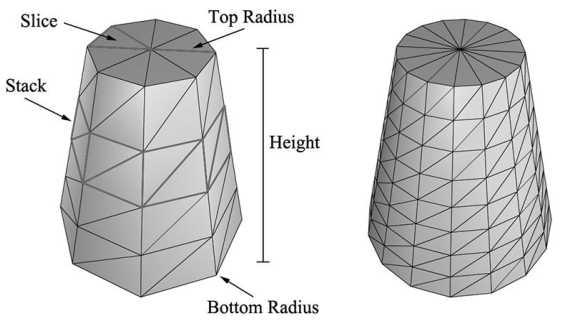
\includegraphics[width=\textwidth]{7-1}
    \centering
    \caption{在此图中,左侧的圆柱体有八个切片和四个堆叠,右侧的圆柱体有十六个切片和八个堆叠。 切片和堆栈控制三角形密度。 请注意,顶部和底部半径可以不同,以便我们可以创建锥形对象,而不仅仅是“纯”圆柱体。}
    \label{fig:7-1}
\end{figure}

%---- 7.4.1.1 ----
\subsubsection{圆柱体边缘几何(Cylinder Side Geometry)}
\begin{flushleft}
我们生成以原点为中心的圆柱体,平行于$y$轴。 从图\ref{fig:7-1}中,所有顶点都位于圆柱体的“环”上,其中有stackCount + 1个环,每个环都有 sliceCount 个(唯一)顶点。 连续环之间的半径差异为$\Delta r=(topRadius - bottomRadius)/ stackCount$。 如果我们从索引为0的底环开始,那么第i个环的半径是$r_{i} = bottomRadius + i\Delta r$,第i个环的高度是 $h_{i}=-\frac{h}{2}+i\Delta h$其中$\Delta h$是堆栈高度,h是圆柱高度。 因此,基本思想是迭代每个环,并生成位于该环上的顶点。 这给出了以下实现:\\
\end{flushleft}
\begin{lstlisting}
GeometryGenerator::MeshData 
GeometryGenerator::CreateCylinder(
    float bottomRadius, 
    float topRadius, 
    float height, 
    uint32 sliceCount, 
    uint32 stackCount)
{
    MeshData meshData;

    //
    // Build Stacks.
    // 

    float stackHeight = height / stackCount;

    // Amount to increment radius as we move up 
    // each stack level from bottom to top.
    float radiusStep = (topRadius - bottomRadius) / stackCount;

    uint32 ringCount = stackCount+1;

    // Compute vertices for each stack ring 
    // starting at the bottom and moving up.
    for(uint32 i = 0; i < ringCount; ++i)
    {
        float y = -0.5f*height + i*stackHeight;
        float r = bottomRadius + i*radiusStep;

        // vertices of ring
        float dTheta = 2.0f*XM_PI/sliceCount;
        for(uint32 j = 0; j <= sliceCount; ++j)
        {
            Vertex vertex;

            float c = cosf(j*dTheta);
            float s = sinf(j*dTheta);

            vertex.Position = XMFLOAT3(r*c, y, r*s);

            vertex.TexC.x = (float)j/sliceCount;
            vertex.TexC.y = 1.0f - (float)i/stackCount;

            // Cylinder can be parameterized as follows, where we introduce v
            // parameter that goes in the same direction as the v tex-coord
            // so that the bitangent goes in the same direction 
            // as the v tex-coord.
            //   Let r0 be the bottom radius and let r1 be the top radius.
            //   y(v) = h - hv for v in [0,1].
            //   r(v) = r1 + (r0-r1)v
            //
            //   x(t, v) = r(v)*cos(t)
            //   y(t, v) = h - hv
            //   z(t, v) = r(v)*sin(t)
            // 
            //  dx/dt = -r(v)*sin(t)
            //  dy/dt = 0
            //  dz/dt = +r(v)*cos(t)
            //
            //  dx/dv = (r0-r1)*cos(t)
            //  dy/dv = -h
            //  dz/dv = (r0-r1)*sin(t)

            // This is unit length.
            vertex.TangentU = XMFLOAT3(-s, 0.0f, c);

            float dr = bottomRadius-topRadius;
            XMFLOAT3 bitangent(dr*c, -height, dr*s);

            XMVECTOR T = XMLoadFloat3(&vertex.TangentU);
            XMVECTOR B = XMLoadFloat3(&bitangent);
            XMVECTOR N = XMVector3Normalize(XMVector3Cross(T, B));
            XMStoreFloat3(&vertex.Normal, N);

            meshData.Vertices.push_back(vertex);
        }
    }
......
\end{lstlisting}
\begin{flushleft}
NOTICE: 观察到每个环的第一个和最后一个顶点在位置上重复,但纹理坐标不重复。 我们必须这样做,以便我们可以正确地将纹理应用于圆柱体。\\
~\\
NOTICE: 实际上GeometryGenerator::CreateCylinder创建了额外的顶点数据,例如法线向量和纹理坐标,这些对未来的演示非常有用。 现在不要担心这些数量。\\
~\\
从图\ref{fig:7-2}可以看出,每个堆栈中的每个切片都有一个四边形(两个三角形)。 图\ref{fig:7-2}显示第$i$个堆栈和第$j$个切片的索引由下式给出:\\
\end{flushleft}
\begin{align*}
\Delta ABC = (i\cdot n+j, (i+1)\cdot n+j,(i+1)\cdot n+j+1)\\
\Delta ACD = (i\cdot n+j, (i+1)\cdot n+j+1,i\cdot n+j+1)
\end{lstlisting}
\begin{align*}
其中n是每个环的顶点数。 所以关键的想法是遍历每个堆栈中的每个切片,并应用上面的公式。\\
\end{flushleft}
\begin{lstlisting}
    // Add one because we duplicate the first and last vertex per ring
    // since the texture coordinates are different.
    uint32 ringVertexCount = sliceCount+1;

    // Compute indices for each stack.
    for(uint32 i = 0; i < stackCount; ++i)
    {
        for(uint32 j = 0; j < sliceCount; ++j)
        {
            meshData.Indices32.push_back(i*ringVertexCount + j);
            meshData.Indices32.push_back((i+1)*ringVertexCount + j);
            meshData.Indices32.push_back((i+1)*ringVertexCount + j+1);

            meshData.Indices32.push_back(i*ringVertexCount + j);
            meshData.Indices32.push_back((i+1)*ringVertexCount + j+1);
            meshData.Indices32.push_back(i*ringVertexCount + j+1);
        }
    }

    BuildCylinderTopCap(bottomRadius, topRadius, height, sliceCount, stackCount, meshData);
    BuildCylinderBottomCap(bottomRadius, topRadius, height, sliceCount, stackCount, meshData);

    return meshData;
}
\end{lstlisting}
\begin{figure}[h]
    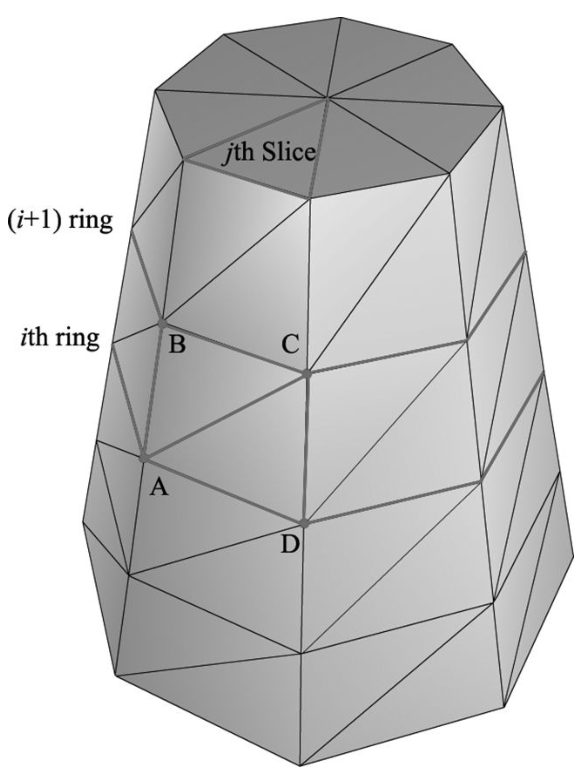
\includegraphics[width=\textwidth]{7-2}
    \centering
    \caption{包含在第$i$个和第$i + 1$个环中的顶点A,B,C,D和第$j$个切片。}
    \label{fig:7-2}
\end{figure}

%---- 7.4.1.2 ----
\subsubsection{顶面底面几何(Cap Geometry)}
\begin{flushleft}
生成顶面几何图形相当于生成顶部和底部环的切片三角形以近似圆形:\\
\end{flushleft}
\begin{lstlisting}
void GeometryGenerator::BuildCylinderTopCap(
    float bottomRadius, 
    float topRadius, 
    float height,
    uint32 sliceCount, 
    uint32 stackCount, 
    MeshData& meshData)
{
    uint32 baseIndex = (uint32)meshData.Vertices.size();

    float y = 0.5f*height;
    float dTheta = 2.0f*XM_PI/sliceCount;

    // Duplicate cap ring vertices because 
    // the texture coordinates and normals differ.
    for(uint32 i = 0; i <= sliceCount; ++i)
    {
        float x = topRadius*cosf(i*dTheta);
        float z = topRadius*sinf(i*dTheta);

        // Scale down by the height to try and 
        // make top cap texture coord area
        // proportional to base.
        float u = x/height + 0.5f;
        float v = z/height + 0.5f;

        meshData.Vertices.push_back(
            Vertex(x, y, z, 
                0.0f, 1.0f, 0.0f, 
                1.0f, 0.0f, 0.0f, 
                u, v));
    }

    // Cap center vertex.
    meshData.Vertices.push_back(
        Vertex(0.0f, y, 0.0f, 
            0.0f, 1.0f, 0.0f, 
            1.0f, 0.0f, 0.0f, 
            0.5f, 0.5f));

    // Index of center vertex.
    uint32 centerIndex = (uint32)meshData.Vertices.size()-1;

    for(uint32 i = 0; i < sliceCount; ++i)
    {
        meshData.Indices32.push_back(centerIndex);
        meshData.Indices32.push_back(baseIndex + i+1);
        meshData.Indices32.push_back(baseIndex + i);
    }
}
\end{lstlisting}
\begin{flushleft}
底面类似。\\
\end{flushleft}

%---- 7.4.2 ----
\subsection{创建球面网格(Generating a Sphere Mesh)}
\begin{flushleft}
我们通过指定半径,切片和堆栈计数来定义球体,如图\ref{fig:7-3}所示。 除了每个环的半径变化是基于三角函数的非线性方式之外,用于生成球体的算法非常类似于圆柱体的算法。 我们将留给读者研究 GeometryGenerator::CreateSphere 代码。 请注意,我们可以应用非均匀缩放世界变换将球体变换为椭圆体。
\end{flushleft}
\begin{figure}[h]
    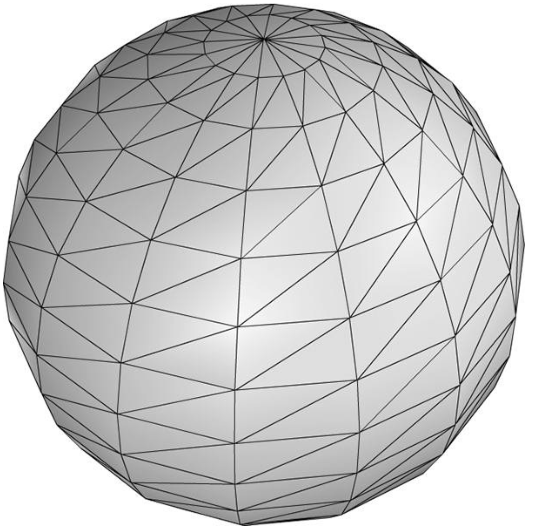
\includegraphics[width=\textwidth]{7-3}
    \centering
    \caption{切片和堆栈的思想也适用于球体来控制曲面细分的级别。}
    \label{fig:7-3}
\end{figure}

%---- 7.4.3 ----
\subsection{创建地圈网格(Generating a Geosphere Mesh)}
\begin{flushleft}
从图\ref{fig:7-3}可以看出,球体的三角形没有相等的面积。 在某些情况下这可能是不合需要的。 地圈使用具有几乎相等面积的三角形以及相等的边长来近似球体(参见图\ref{fig:7-4})。
\end{flushleft}

\begin{figure}[h]
    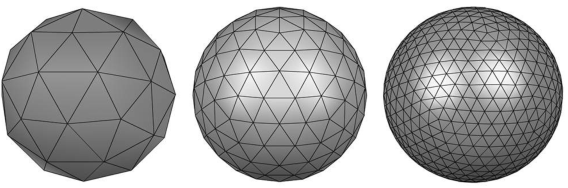
\includegraphics[width=\textwidth]{7-4}
    \centering
    \caption{通过重复细分和重投影到球体上来近似地圈。}
    \label{fig:7-4}
\end{figure}

\begin{flushleft}
为了生成地圈,我们从二十面体开始,细分三角形,然后将新顶点投影到具有给定半径的球体上。 我们可以重复此过程以改进曲面细分。\\
图\ref{fig:7-5}显示了如何将三角形细分为四个相等大小的三角形。 只需沿原始三角形的边缘取中点即可找到新的顶点。 然后,通过将顶点投影到单位球上然后标量乘以$r: v^{'}=r \frac{v}{||v||}$,可以将新顶点投影到半径为$r$的球体上
\end{flushleft}

\begin{figure}[h]
    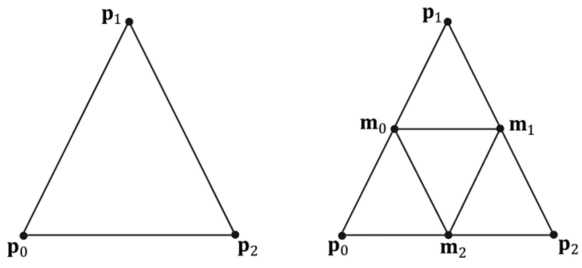
\includegraphics[width=\textwidth]{7-5}
    \centering
    \caption{将三角形细分为四个相等面积的三角形。}
    \label{fig:7-5}
\end{figure}

\begin{flushleft}
代码如下:\\
\end{flushleft}
\begin{lstlisting}
GeometryGenerator::MeshData 
GeometryGenerator::CreateGeosphere(
    float radius, 
    uint32 numSubdivisions)
{
    MeshData meshData;

    // Put a cap on the number of subdivisions.
    numSubdivisions = std::min<uint32>(numSubdivisions, 6u);

    // Approximate a sphere by tessellating an icosahedron.

    const float X = 0.525731f; 
    const float Z = 0.850651f;

    XMFLOAT3 pos[12] = 
    {
        XMFLOAT3(-X, 0.0f, Z),  XMFLOAT3(X, 0.0f, Z),  
        XMFLOAT3(-X, 0.0f, -Z), XMFLOAT3(X, 0.0f, -Z),    
        XMFLOAT3(0.0f, Z, X),   XMFLOAT3(0.0f, Z, -X), 
        XMFLOAT3(0.0f, -Z, X),  XMFLOAT3(0.0f, -Z, -X),    
        XMFLOAT3(Z, X, 0.0f),   XMFLOAT3(-Z, X, 0.0f), 
        XMFLOAT3(Z, -X, 0.0f),  XMFLOAT3(-Z, -X, 0.0f)
    };

    uint32 k[60] =
    {
        1,4,0,  4,9,0,  4,5,9,  8,5,4,  1,8,4,    
        1,10,8, 10,3,8, 8,3,5,  3,2,5,  3,7,2,    
        3,10,7, 10,6,7, 6,11,7, 6,0,11, 6,1,0, 
        10,1,6, 11,0,9, 2,11,9, 5,2,9,  11,2,7 
    };

    meshData.Vertices.resize(12);
    meshData.Indices32.assign(&k[0], &k[60]);

    for(uint32 i = 0; i < 12; ++i)
        meshData.Vertices[i].Position = pos[i];

    for(uint32 i = 0; i < numSubdivisions; ++i)
        Subdivide(meshData);

    // Project vertices onto sphere and scale.
    for(uint32 i = 0; i < meshData.Vertices.size(); ++i)
    {
        // Project onto unit sphere.
        XMVECTOR n = XMVector3Normalize(XMLoadFloat3(&meshData.Vertices[i].Position));

        // Project onto sphere.
        XMVECTOR p = radius*n;

        XMStoreFloat3(&meshData.Vertices[i].Position, p);
        XMStoreFloat3(&meshData.Vertices[i].Normal, n);

        // Derive texture coordinates from spherical coordinates.
        float theta = atan2f(meshData.Vertices[i].Position.z, 
                             meshData.Vertices[i].Position.x);

        // Put in [0, 2pi].
        if(theta < 0.0f)
            theta += XM_2PI;

        float phi = acosf(meshData.Vertices[i].Position.y / radius);

        meshData.Vertices[i].TexC.x = theta/XM_2PI;
        meshData.Vertices[i].TexC.y = phi/XM_PI;

        // Partial derivative of P with respect to theta
        meshData.Vertices[i].TangentU.x = -radius*sinf(phi)*sinf(theta);
        meshData.Vertices[i].TangentU.y = 0.0f;
        meshData.Vertices[i].TangentU.z = +radius*sinf(phi)*cosf(theta);

        XMVECTOR T = XMLoadFloat3(&meshData.Vertices[i].TangentU);
        XMStoreFloat3(&meshData.Vertices[i].TangentU, XMVector3Normalize(T));
    }

    return meshData;
}
\end{lstlisting}

%---- 7.5 ----
\section{Shapes Demo}
\begin{flushleft}
为了演示我们的球体和圆柱体生成代码,我们实现了如图\ref{fig:7-6}所示的 "Shapes" 演示。 此外,您还将获得在场景中定位和绘制多个对象的经验(即,创建多个世界变换矩阵)。 此外,我们将所有场景几何体放在一个大顶点和索引缓冲区中。 然后我们将使用 DrawIndexedInstanced 方法一次绘制一个对象(因为需要在对象之间更改世界矩阵); 因此,您将看到使用 DrawIndexedInstanced 的 StartIndexLocation 和 BaseVertexLocation 参数的示例。\\
\end{flushleft}

\begin{figure}[h]
    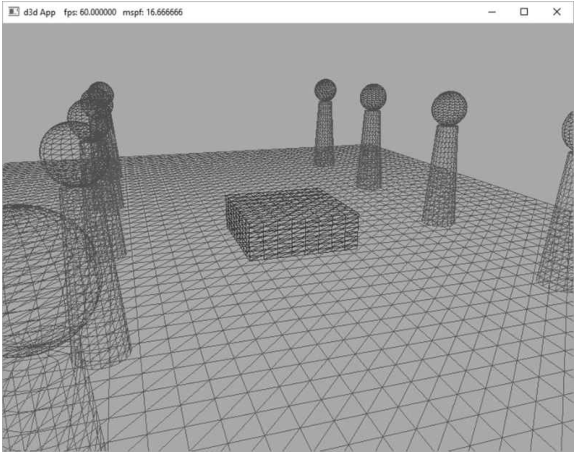
\includegraphics[width=\textwidth]{7-6}
    \centering
    \caption{"Shapes"演示的截图}
    \label{fig:7-6}
\end{figure}

%---- 7.5.1 ----
\subsection{顶点和顶点缓冲区(Vertex and Index Buffers)}
\begin{flushleft}
如图\ref{fig:7-6}所示,在本演示中,我们绘制了一个框,网格(grid),圆柱体和球体。 尽管我们在此演示中绘制了多个球体和圆柱体,但我们只需要一个球体和圆柱体几何体的副本。 我们只是多次重绘相同的球体和圆柱网格,但是使用不同的世界矩阵; 这是几何实例化的一个例子,它可以节省内存。\\
我们将所有网格顶点和索引打包到一个顶点和索引缓冲区中。 这是通过连接顶点和索引数组来完成的。 这意味着当我们绘制一个对象时,我们只绘制顶点和索引缓冲区的子集。 为了使用 ID3D12CommandList::DrawIndexedInstanced 仅绘制几何的子集,我们需要知道三个量(回想一下图\ref{fig:6-3}以及第6章中关于它的讨论)。 我们需要知道连接索引缓冲区中对象的起始索引,它的索引计数,我们需要知道基本顶点位置 - 对象相对于连接顶点缓冲区的第一个顶点的索引。 回想一下,基本顶点位置是在提取顶点之前添加到绘制调用中的索引的整数值,以便索引引用连接顶点缓冲区中的正确子集。 (另见第5章的练习2)\\

下面的代码显示了如何创建几何缓冲区,如何缓存必要的图纸数量以及如何绘制对象。
\end{flushleft}

\begin{lstlisting}
void ShapesApp::BuildShapeGeometry()
{
    GeometryGenerator geoGen;
    GeometryGenerator::MeshData box = 
        geoGen.CreateBox(1.5f, 0.5f, 1.5f, 3);
    GeometryGenerator::MeshData grid = 
        geoGen.CreateGrid(20.0f, 30.0f, 60, 40);
    GeometryGenerator::MeshData sphere = 
        geoGen.CreateSphere(0.5f, 20, 20);
    GeometryGenerator::MeshData cylinder = 
        geoGen.CreateCylinder(0.5f, 0.3f, 3.0f, 20, 20);

    //
    // We are concatenating all the geometry 
    // into one big vertex/index buffer.  So
    // define the regions in the buffer each submesh covers.
    //

    // Cache the vertex offsets to each object 
    // in the concatenated vertex buffer.
    UINT boxVertexOffset = 0;
    UINT gridVertexOffset = (UINT)box.Vertices.size();
    UINT sphereVertexOffset = gridVertexOffset + 
                           (UINT)grid.Vertices.size();
    UINT cylinderVertexOffset = sphereVertexOffset + 
                           (UINT)sphere.Vertices.size();

    // Cache the starting index for each object in the concatenated index buffer.
    UINT boxIndexOffset = 0;
    UINT gridIndexOffset = (UINT)box.Indices32.size();
    UINT sphereIndexOffset = gridIndexOffset + 
                           (UINT)grid.Indices32.size();
    UINT cylinderIndexOffset = sphereIndexOffset + 
                           (UINT)sphere.Indices32.size();

    // Define the SubmeshGeometry that cover different 
    // regions of the vertex/index buffers.

    SubmeshGeometry boxSubmesh;
    boxSubmesh.IndexCount = (UINT)box.Indices32.size();
    boxSubmesh.StartIndexLocation = boxIndexOffset;
    boxSubmesh.BaseVertexLocation = boxVertexOffset;

    SubmeshGeometry gridSubmesh;
    gridSubmesh.IndexCount = (UINT)grid.Indices32.size();
    gridSubmesh.StartIndexLocation = gridIndexOffset;
    gridSubmesh.BaseVertexLocation = gridVertexOffset;

    SubmeshGeometry sphereSubmesh;
    sphereSubmesh.IndexCount = (UINT)sphere.Indices32.size();
    sphereSubmesh.StartIndexLocation = sphereIndexOffset;
    sphereSubmesh.BaseVertexLocation = sphereVertexOffset;

    SubmeshGeometry cylinderSubmesh;
    cylinderSubmesh.IndexCount = (UINT)cylinder.Indices32.size();
    cylinderSubmesh.StartIndexLocation = cylinderIndexOffset;
    cylinderSubmesh.BaseVertexLocation = cylinderVertexOffset;

    //
    // Extract the vertex elements we are 
    // interested in and pack the
    // vertices of all the meshes into 
    // one vertex buffer.
    //

    auto totalVertexCount =
        box.Vertices.size() +
        grid.Vertices.size() +
        sphere.Vertices.size() +
        cylinder.Vertices.size();

    std::vector<Vertex> vertices(totalVertexCount);

    UINT k = 0;
    for(size_t i = 0; i < box.Vertices.size(); ++i, ++k)
    {
        vertices[k].Pos = box.Vertices[i].Position;
        vertices[k].Color = XMFLOAT4(DirectX::Colors::DarkGreen);
    }

    for(size_t i = 0; i < grid.Vertices.size(); ++i, ++k)
    {
        vertices[k].Pos = grid.Vertices[i].Position;
        vertices[k].Color = XMFLOAT4(DirectX::Colors::ForestGreen);
    }

    for(size_t i = 0; i < sphere.Vertices.size(); ++i, ++k)
    {
        vertices[k].Pos = sphere.Vertices[i].Position;
        vertices[k].Color = XMFLOAT4(DirectX::Colors::Crimson);
    }

    for(size_t i = 0; i < cylinder.Vertices.size(); ++i, ++k)
    {
        vertices[k].Pos = cylinder.Vertices[i].Position;
        vertices[k].Color = XMFLOAT4(DirectX::Colors::SteelBlue);
    }

    std::vector<std::uint16_t> indices;
    indices.insert(indices.end(), 
                   std::begin(box.GetIndices16()), 
                   std::end(box.GetIndices16()));
    indices.insert(indices.end(), 
                   std::begin(grid.GetIndices16()), 
                   std::end(grid.GetIndices16()));
    indices.insert(indices.end(), 
                   std::begin(sphere.GetIndices16()), 
                   std::end(sphere.GetIndices16()));
    indices.insert(indices.end(), 
                   std::begin(cylinder.GetIndices16()), 
                   std::end(cylinder.GetIndices16()));

    const UINT vbByteSize = (UINT)vertices.size() * 
                            sizeof(Vertex);
    const UINT ibByteSize = (UINT)indices.size() * 
                            sizeof(std::uint16_t);

    auto geo = std::make_unique<MeshGeometry>();
    geo->Name = "shapeGeo";

    ThrowIfFailed(D3DCreateBlob(vbByteSize, &geo->VertexBufferCPU));
    CopyMemory(geo->VertexBufferCPU->GetBufferPointer(), 
                    vertices.data(), 
                    vbByteSize);

    ThrowIfFailed(D3DCreateBlob(ibByteSize, &geo->IndexBufferCPU));
    CopyMemory(geo->IndexBufferCPU->GetBufferPointer(), 
                    indices.data(), 
                    ibByteSize);

    geo->VertexBufferGPU = d3dUtil::CreateDefaultBuffer(md3dDevice.Get(),
        mCommandList.Get(), vertices.data(), 
        vbByteSize, geo->VertexBufferUploader);

    geo->IndexBufferGPU = d3dUtil::CreateDefaultBuffer(md3dDevice.Get(),
        mCommandList.Get(), indices.data(), 
        ibByteSize, geo->IndexBufferUploader);

    geo->VertexByteStride = sizeof(Vertex);
    geo->VertexBufferByteSize = vbByteSize;
    geo->IndexFormat = DXGI_FORMAT_R16_UINT;
    geo->IndexBufferByteSize = ibByteSize;

    geo->DrawArgs["box"] = boxSubmesh;
    geo->DrawArgs["grid"] = gridSubmesh;
    geo->DrawArgs["sphere"] = sphereSubmesh;
    geo->DrawArgs["cylinder"] = cylinderSubmesh;

    mGeometries[geo->Name] = std::move(geo);
}
\end{lstlisting}

\begin{flushleft}
在上面方法的最后一行中使用的 mGeometries 变量定义如下:\\
\end{flushleft}

\begin{lstlisting}
std::unordered_map<std::string, 
            std::unique_ptr<MeshGeometry>> mGeometries;
\end{lstlisting}

\begin{flushleft}
这是我们在本书其余部分使用的常见模式。 为每个几何体,PSO,纹理,着色器等创建新的变量名称很麻烦,因此我们使用无序地图进行常量时间查找并按名称引用我们的对象。 以下是一些例子:\\
\end{flushleft}

\begin{lstlisting}
std::unordered_map<std::string,
    std::unique_ptr<MeshGeometry>> mGeometries;
std::unordered_map<std::string, ComPtr<ID3DBlob>>
    mShaders;
std::unordered_map<std::string,
    ComPtr<ID3D12PipelineState>> mPSOs;
\end{lstlisting}

%---- 7.5.2 ----
\subsection{渲染项(Render Items)}
\begin{flushleft}
我们现在定义场景渲染项。 观察所有渲染项如何共享相同的 MeshGeometry,并使用 DrawArgs 获取 DrawIndexedInstanced 参数以绘制顶点/索引缓冲区的子区域。\\
\end{flushleft}

\begin{lstlisting}
// ShapesApp member variable.
std::vector<std::unique_ptr<RenderItem>> mAllRitems;
std::vector<RenderItem*> mOpaqueRitems;

void ShapesApp::BuildRenderItems()
{
    auto boxRitem = std::make_unique<RenderItem>();
    XMStoreFloat4x4(&boxRitem->World, 
         XMMatrixScaling(2.0f, 2.0f, 2.0f)*
         XMMatrixTranslation(0.0f, 0.5f, 0.0f));

    boxRitem->ObjCBIndex = 0;
    boxRitem->Geo = mGeometries["shapeGeo"].get();
    boxRitem->PrimitiveType = D3D_PRIMITIVE_TOPOLOGY_TRIANGLELIST;
    boxRitem->IndexCount = boxRitem->Geo->
        DrawArgs["box"].IndexCount;
    boxRitem->StartIndexLocation = boxRitem->Geo->
        DrawArgs["box"].StartIndexLocation;
    boxRitem->BaseVertexLocation = boxRitem->Geo->
        DrawArgs["box"].BaseVertexLocation;
    mAllRitems.push_back(std::move(boxRitem));

    auto gridRitem = std::make_unique<RenderItem>();
    gridRitem->World = MathHelper::Identity4x4();
    gridRitem->ObjCBIndex = 1;
    gridRitem->Geo = mGeometries["shapeGeo"].get();
    gridRitem->PrimitiveType = D3D_PRIMITIVE_TOPOLOGY_TRIANGLELIST;
    gridRitem->IndexCount = gridRitem->Geo->
        DrawArgs["grid"].IndexCount;
    gridRitem->StartIndexLocation = gridRitem->Geo->
        DrawArgs["grid"].StartIndexLocation;
    gridRitem->BaseVertexLocation = gridRitem->Geo->
        DrawArgs["grid"].BaseVertexLocation;
    mAllRitems.push_back(std::move(gridRitem));

    UINT objCBIndex = 2;
    for(int i = 0; i < 5; ++i)
    {
        auto leftCylRitem = std::make_unique<RenderItem>();
        auto rightCylRitem = std::make_unique<RenderItem>();
        auto leftSphereRitem = std::make_unique<RenderItem>();
        auto rightSphereRitem = std::make_unique<RenderItem>();

        XMMATRIX leftCylWorld = XMMatrixTranslation(
            -5.0f, 1.5f, -10.0f + i*5.0f);
        XMMATRIX rightCylWorld = XMMatrixTranslation(
            +5.0f, 1.5f, -10.0f + i*5.0f);

        XMMATRIX leftSphereWorld = XMMatrixTranslation(
            -5.0f, 3.5f, -10.0f + i*5.0f);
        XMMATRIX rightSphereWorld = XMMatrixTranslation(
            +5.0f, 3.5f, -10.0f + i*5.0f);

        XMStoreFloat4x4(&leftCylRitem->World, 
            rightCylWorld);
        leftCylRitem->ObjCBIndex = objCBIndex++;
        leftCylRitem->Geo = mGeometries["shapeGeo"].get();
        leftCylRitem->PrimitiveType = 
            D3D_PRIMITIVE_TOPOLOGY_TRIANGLELIST;
        leftCylRitem->IndexCount = leftCylRitem->Geo->
            DrawArgs["cylinder"].IndexCount;
        leftCylRitem->StartIndexLocation = leftCylRitem->Geo->
            DrawArgs["cylinder"].StartIndexLocation;
        leftCylRitem->BaseVertexLocation = leftCylRitem->Geo->
            DrawArgs["cylinder"].BaseVertexLocation;

        XMStoreFloat4x4(&rightCylRitem->World, leftCylWorld);
        rightCylRitem->ObjCBIndex = objCBIndex++;
        rightCylRitem->Geo = mGeometries["shapeGeo"].get();
        rightCylRitem->PrimitiveType = 
            D3D_PRIMITIVE_TOPOLOGY_TRIANGLELIST;
        rightCylRitem->IndexCount = rightCylRitem->Geo->
            DrawArgs["cylinder"].IndexCount;
        rightCylRitem->StartIndexLocation = rightCylRitem->Geo->
            DrawArgs["cylinder"].StartIndexLocation;
        rightCylRitem->BaseVertexLocation = rightCylRitem->Geo->
            DrawArgs["cylinder"].BaseVertexLocation;

        XMStoreFloat4x4(&leftSphereRitem->World, leftSphereWorld);
        leftSphereRitem->ObjCBIndex = objCBIndex++;
        leftSphereRitem->Geo = mGeometries["shapeGeo"].get();
        leftSphereRitem->PrimitiveType = 
            D3D_PRIMITIVE_TOPOLOGY_TRIANGLELIST;
        leftSphereRitem->IndexCount = leftSphereRitem->Geo->
            DrawArgs["sphere"].IndexCount;
        leftSphereRitem->StartIndexLocation = leftSphereRitem->Geo->
            DrawArgs["sphere"].StartIndexLocation;
        leftSphereRitem->BaseVertexLocation = leftSphereRitem->Geo->
            DrawArgs["sphere"].BaseVertexLocation;

        XMStoreFloat4x4(&rightSphereRitem->World, rightSphereWorld);
        rightSphereRitem->ObjCBIndex = objCBIndex++;
        rightSphereRitem->Geo = mGeometries["shapeGeo"].get();
        rightSphereRitem->PrimitiveType = 
            D3D_PRIMITIVE_TOPOLOGY_TRIANGLELIST;
        rightSphereRitem->IndexCount = rightSphereRitem->Geo->
            DrawArgs["sphere"].IndexCount;
        rightSphereRitem->StartIndexLocation = rightSphereRitem->Geo->
            DrawArgs["sphere"].StartIndexLocation;
        rightSphereRitem->BaseVertexLocation = rightSphereRitem->Geo->
            DrawArgs["sphere"].BaseVertexLocation;

        mAllRitems.push_back(std::move(leftCylRitem));
        mAllRitems.push_back(std::move(rightCylRitem));
        mAllRitems.push_back(std::move(leftSphereRitem));
        mAllRitems.push_back(std::move(rightSphereRitem));
    }

    // All the render items are opaque.
    for(auto& e : mAllRitems)
        mOpaqueRitems.push_back(e.get());
}
\end{lstlisting}

%---- 7.5.3 ----
\subsection{帧资源和常量缓冲视图(Frame Resources and Constant Buffer Views)}
\begin{flushleft}
回想一下,我们有一个 FrameResources 的向量,每个 FrameResource 都有一个上传缓冲区,用于存储场景中每个渲染项的传递常量和常量缓冲区。
\end{flushleft}

\begin{lstlisting}
std::unique_ptr<UploadBuffer<PassConstants>> PassCB = nullptr;
std::unique_ptr<UploadBuffer<ObjectConstants>> ObjectCB = nullptr;
\end{lstlisting}

\begin{flushleft}
如果我们有3个帧资源和 $n$ 个渲染项,那么我们有 $3n$ 个对象\footnote{原文是:"then we have three 3n object constant
buffers",是错误的}常量缓冲区和3个传递常量缓冲区。 因此,我们需要$3(n+1)$个常量缓冲区视图(CBV)。 所以,我们需要修改我们的CBV堆以包含其他描述符:\\
\end{flushleft}

\begin{lstlisting}
void ShapesApp::BuildDescriptorHeaps()
{
    UINT objCount = (UINT)mOpaqueRitems.size();

    // Need a CBV descriptor for each object for each frame resource,
    // +1 for the perPass CBV for each frame resource.
    UINT numDescriptors = (objCount+1) * 3;

    // Save an offset to the start of the pass CBVs.  
    // These are the last 3 descriptors.
    mPassCbvOffset = objCount * gNumFrameResources;

    D3D12_DESCRIPTOR_HEAP_DESC cbvHeapDesc;
    cbvHeapDesc.NumDescriptors = numDescriptors;
    cbvHeapDesc.Type = D3D12_DESCRIPTOR_HEAP_TYPE_CBV_SRV_UAV;
    cbvHeapDesc.Flags = D3D12_DESCRIPTOR_HEAP_FLAG_SHADER_VISIBLE;
    cbvHeapDesc.NodeMask = 0;
    ThrowIfFailed(md3dDevice->CreateDescriptorHeap(&cbvHeapDesc,
        IID_PPV_ARGS(&mCbvHeap)));
}
\end{lstlisting}

\begin{flushleft}
现在,我们可以使用以下代码填充CBV堆,其中描述符$0$到$n-1$包含第$0$帧资源的对象CBV,描述符$n$到$2n-1$包含第$1$帧资源的对象CBV,描述符$2n$到$3n-1$ 包含第二帧资源的对象CBV,描述符$3n$,$3n + 1$和$3n + 2$分别包含第$0$帧,第$1$帧和第$2$帧资源的传递CBV:\\
\end{flushleft}

\begin{lstlisting}
void ShapesApp::BuildConstantBufferViews()
{
    UINT objCBByteSize = d3dUtil::CalcConstantBufferByteSize(
            sizeof(ObjectConstants));

    UINT objCount = (UINT)mOpaqueRitems.size();

    // Need a CBV descriptor for each object for each frame resource.
    for(int frameIndex = 0; 
        frameIndex < gNumFrameResources; 
        ++frameIndex)
    {
        auto objectCB = mFrameResources[frameIndex]->
            ObjectCB->Resource();
        for(UINT i = 0; i < objCount; ++i)
        {
            D3D12_GPU_VIRTUAL_ADDRESS cbAddress = 
                objectCB->GetGPUVirtualAddress();

            // Offset to the ith object constant buffer in the buffer.
            cbAddress += i*objCBByteSize;

            // Offset to the object cbv in the descriptor heap.
            int heapIndex = frameIndex*objCount + i;
            auto handle = CD3DX12_CPU_DESCRIPTOR_HANDLE(mCbvHeap->
                GetCPUDescriptorHandleForHeapStart());
            handle.Offset(heapIndex, mCbvSrvUavDescriptorSize);

            D3D12_CONSTANT_BUFFER_VIEW_DESC cbvDesc;
            cbvDesc.BufferLocation = cbAddress;
            cbvDesc.SizeInBytes = objCBByteSize;

            md3dDevice->CreateConstantBufferView(&cbvDesc, handle);
        }
    }

    UINT passCBByteSize = d3dUtil::CalcConstantBufferByteSize(
        sizeof(PassConstants));

    // Last three descriptors are the pass CBVs for each frame resource.
    for(int frameIndex = 0; frameIndex < gNumFrameResources; ++frameIndex)
    {
        auto passCB = mFrameResources[frameIndex]->PassCB->Resource();
        D3D12_GPU_VIRTUAL_ADDRESS cbAddress = passCB->GetGPUVirtualAddress();

        // Offset to the pass cbv in the descriptor heap.
        int heapIndex = mPassCbvOffset + frameIndex;
        auto handle = CD3DX12_CPU_DESCRIPTOR_HANDLE(mCbvHeap->
            GetCPUDescriptorHandleForHeapStart());
        handle.Offset(heapIndex, mCbvSrvUavDescriptorSize);

        D3D12_CONSTANT_BUFFER_VIEW_DESC cbvDesc;
        cbvDesc.BufferLocation = cbAddress;
        cbvDesc.SizeInBytes = passCBByteSize;
        
        md3dDevice->CreateConstantBufferView(&cbvDesc, handle);
    }
}
\end{lstlisting}

\begin{flushleft}
回想一下,我们可以使用 ID3D12DescriptorHeap::GetCPUDescriptorHandleForHeapStart 方法获取堆中第一个描述符的句柄。 但是,现在我们的堆有多个描述符,这个方法已不再适用。 我们需要能够偏移到堆中的其他描述符。 为此,我们需要知道要在堆中递增的大小以获取到下一个描述符。 这是特定于硬件的,因此我们必须从设备查询此信息,这取决于堆类型。 回想一下,我们的 D3DApp 类缓存了这些信息:\\
\end{flushleft}

\begin{lstlisting}
mRtvDescriptorSize = md3dDevice->
    GetDescriptorHandleIncrementSize(
    D3D12_DESCRIPTOR_HEAP_TYPE_RTV);
mDsvDescriptorSize = md3dDevice->
    GetDescriptorHandleIncrementSize(
    D3D12_DESCRIPTOR_HEAP_TYPE_DSV);
mCbvSrvUavDescriptorSize = md3dDevice->
    GetDescriptorHandleIncrementSize(
    D3D12_DESCRIPTOR_HEAP_TYPE_CBV_SRV_UAV);
\end{lstlisting}

\begin{flushleft}
一旦我们知道描述符增量大小,我们就可以使用两个 CD3DX12\_CPU\_DESCRIPTOR\_HANDLE::Offset 方法之一来通过 n 个描述符来偏移句柄:\\
\end{flushleft}

\begin{lstlisting}
// Specify the number of descriptors to offset times 
// the descriptor Offset by n descriptors:
CD3DX12_CPU_DESCRIPTOR_HANDLE handle = mCbvHeap->
    GetCPUDescriptorHandleForHeapStart();
handle.Offset(n * mCbvSrvDescriptorSize);

// Or equivalently, specify the number of 
// descriptors to offset, followed by 
// the descriptor increment size:
CD3DX12_CPU_DESCRIPTOR_HANDLE handle = mCbvHeap->
    GetCPUDescriptorHandleForHeapStart();
handle.Offset(n, mCbvSrvDescriptorSize);
\end{lstlisting}

\begin{flushleft}
NOTICE: CD3DX12\_GPU\_DESCRIPTOR\_HANDLE 有相同的 Offset 方法。
\end{flushleft}


%---- 7.5.4 ----
\subsection{绘制场景(Draw the Scene)}
\begin{flushleft}
最后我们可以绘制渲染项。 也许唯一棘手的部分是通过程序偏移到堆中(我们想要绘制的对象的)正确CBV。 注意渲染项如何将索引存储到与渲染项关联的常量缓冲区的。\\
\end{flushleft}

\begin{lstlisting}
void ShapesApp::DrawRenderItems(
    ID3D12GraphicsCommandList* cmdList, 
    const std::vector<RenderItem*>& ritems)
{
    UINT objCBByteSize = d3dUtil::CalcConstantBufferByteSize(
        sizeof(ObjectConstants));
 
    auto objectCB = mCurrFrameResource->ObjectCB->Resource();

    // For each render item...
    for(size_t i = 0; i < ritems.size(); ++i)
    {
        auto ri = ritems[i];

        cmdList->IASetVertexBuffers(0, 1, 
            &ri->Geo->VertexBufferView());
        cmdList->IASetIndexBuffer(
            &ri->Geo->IndexBufferView());
        cmdList->IASetPrimitiveTopology(
            ri->PrimitiveType);

        // Offset to the CBV in the descriptor heap for 
        // this object and for this frame resource.
        UINT cbvIndex = mCurrFrameResourceIndex*
            (UINT)mOpaqueRitems.size() + ri->ObjCBIndex;
        auto cbvHandle = CD3DX12_GPU_DESCRIPTOR_HANDLE(mCbvHeap->
            GetGPUDescriptorHandleForHeapStart());
        cbvHandle.Offset(cbvIndex, mCbvSrvUavDescriptorSize);

        cmdList->SetGraphicsRootDescriptorTable(0, cbvHandle);

        cmdList->DrawIndexedInstanced(ri->IndexCount, 1, 
            ri->StartIndexLocation, ri->BaseVertexLocation, 0);
    }
}
\end{lstlisting}

\begin{flushleft}
DrawRenderItems 方法由 Draw 调用:\\
\end{flushleft}

\begin{lstlisting}
void ShapesApp::Draw(const GameTimer& gt)
{
    auto cmdListAlloc = mCurrFrameResource->CmdListAlloc;

    // Reuse the memory associated with command recording.
    // We can only reset when the associated command 
    // lists have finished execution on the GPU.
    ThrowIfFailed(cmdListAlloc->Reset());

    // A command list can be reset after it has 
    // been added to the command queue via ExecuteCommandList.
    // Reusing the command list reuses memory.
    if(mIsWireframe)
    {
        ThrowIfFailed(mCommandList->Reset(
            cmdListAlloc.Get(), 
            mPSOs["opaque_wireframe"].Get()));
    }
    else
    {
        ThrowIfFailed(mCommandList->Reset(
            cmdListAlloc.Get(), 
            mPSOs["opaque"].Get()));
    }

    mCommandList->RSSetViewports(1, &mScreenViewport);
    mCommandList->RSSetScissorRects(1, &mScissorRect);

    // Indicate a state transition on the resource usage.
    mCommandList->ResourceBarrier(1, 
        &CD3DX12_RESOURCE_BARRIER::Transition(
            CurrentBackBuffer(),
            D3D12_RESOURCE_STATE_PRESENT, 
            D3D12_RESOURCE_STATE_RENDER_TARGET));

    // Clear the back buffer and depth buffer.
    mCommandList->ClearRenderTargetView(CurrentBackBufferView(), 
        Colors::LightSteelBlue, 0, nullptr);
    mCommandList->ClearDepthStencilView(DepthStencilView(), 
        D3D12_CLEAR_FLAG_DEPTH | D3D12_CLEAR_FLAG_STENCIL, 
        1.0f, 0, 0, nullptr);

    // Specify the buffers we are going to render to.
    mCommandList->OMSetRenderTargets(1, &CurrentBackBufferView(), 
        true, &DepthStencilView());

    ID3D12DescriptorHeap* descriptorHeaps[] = { mCbvHeap.Get() };
    mCommandList->SetDescriptorHeaps(
        _countof(descriptorHeaps), 
        descriptorHeaps);

	mCommandList->SetGraphicsRootSignature(mRootSignature.Get());

    int passCbvIndex = mPassCbvOffset + mCurrFrameResourceIndex;
    auto passCbvHandle = CD3DX12_GPU_DESCRIPTOR_HANDLE(
        mCbvHeap->GetGPUDescriptorHandleForHeapStart());
    passCbvHandle.Offset(passCbvIndex, mCbvSrvUavDescriptorSize);
    mCommandList->SetGraphicsRootDescriptorTable(1, passCbvHandle);

    DrawRenderItems(mCommandList.Get(), mOpaqueRitems);

    // Indicate a state transition on the resource usage.
    mCommandList->ResourceBarrier(1, 
        &CD3DX12_RESOURCE_BARRIER::Transition(
            CurrentBackBuffer(),
            D3D12_RESOURCE_STATE_RENDER_TARGET, 
            D3D12_RESOURCE_STATE_PRESENT));

    // Done recording commands.
    ThrowIfFailed(mCommandList->Close());

    // Add the command list to the queue for execution.
    ID3D12CommandList* cmdsLists[] = { mCommandList.Get() };
    mCommandQueue->ExecuteCommandLists(_countof(cmdsLists), cmdsLists);

    // Swap the back and front buffers
    ThrowIfFailed(mSwapChain->Present(0, 0));
    mCurrBackBuffer = (mCurrBackBuffer + 1) % SwapChainBufferCount;

    // Advance the fence value to mark commands 
    // up to this fence point.
    mCurrFrameResource->Fence = ++mCurrentFence;
    
    // Add an instruction to the command queue 
    // to set a new fence point. 
    // Because we are on the GPU timeline, 
    // the new fence point won't be 
    // set until the GPU finishes processing all
    // the commands prior to this Signal().
    mCommandQueue->Signal(mFence.Get(), mCurrentFence);
}
\end{lstlisting}

%---- 7.6 ----
\section{更多关于根签名(More on Root Signatures)}
\begin{flushleft}
我们在前一章的第6.6.5节中介绍了根签名。 根签名定义在发出绘制调用之前需要将哪些资源绑定到管道以及这些资源如何映射到着色器输入寄存器。 需要绑定哪些资源取决于当前着色器程序所期望的资源。 创建PSO时,将验证根签名和着色器程序组合。
\end{flushleft}

%---- 7.6.1 ----
\subsection{根参数(Root Parameters)}
\begin{flushleft}
回想一下,根签名是由一组根参数定义的。 到目前为止,我们只创建了一个存储描述符表的根参数。 但是,root参数实际上可以是以下三种类型之一:\\
\end{flushleft}

\begin{itemize}
  \item 描述符表(Descriptor Table): 期望描述符表引用堆中的连续范围,该范围标识要绑定的资源。
  \item 根描述符(Root Descriptor | Inline Descriptor): 期望直接设置描述符以识别要绑定的资源; 描述符不需要在堆中。 只有 CBV 到常量缓冲区,SRV/UAV 到缓冲区可以绑定为根描述符。 特别是,这意味着 SRV 到纹理不能绑定为根描述符。
  \item 根常量(Root constant): 期望直接绑定的32位常量值列表。
\end{itemize}

\begin{flushleft}
出于性能考虑,可以将64个DWORD限制在根签名中。 这三种根参数具有以下内存消耗:\\
\end{flushleft}

\begin{itemize}
  \item 描述符表(Descriptor Table): 1 DWORD
  \item 根描述符(Root Descriptor): 2 DWORDs
  \item 根常量(Root constant): 每 32-bit 常量 1 DWORD
\end{itemize}

\begin{flushleft}
我们可以创建一个任意的根签名,只要我们不超过64个DWORD限制。 根常量非常方便,但它们的成本很快就会增加。 例如,如果我们需要的唯一常量数据是世界视图投影矩阵,我们可以使用16个根常量来存储它,这将使我们不需要涉及常量缓冲区和CBV堆。 但是,这会占我们根签名预算的四分之一。 使用根描述符只能是两个DWORD,描述符表只有一个DWORD。 随着我们的应用程序变得越来越复杂,我们的常量缓冲区数据将变得越来越大,并且我们不太可能只使用根常量。 在实际应用程序中,您可能会使用所有三种类型的根参数的组合。\\
在代码中,通过填写 CD3DX12\_ROOT\_PARAMETER 结构来描述根参数。 正如我们在 CD3DX 代码中看到的那样,CD3DX12\_ROOT\_PARAMETER 扩展了 D3D12\_ROOT\_PARAMETER 并添加了一些辅助初始化函数。\\
\end{flushleft}

\begin{lstlisting}
typedef struct D3D12_ROOT_PARAMETER
{
    D3D12_ROOT_PARAMETER_TYPE ParameterType;
    union
    {
        D3D12_ROOT_DESCRIPTOR_TABLE DescriptorTable;
        D3D12_ROOT_CONSTANTS Constants;
        D3D12_ROOT_DESCRIPTOR Descriptor;
    };
    D3D12_SHADER_VISIBILITY ShaderVisibility;
} D3D12_ROOT_PARAMETER;
\end{lstlisting}

\begin{itemize}
  \item 1.ParameterType: 以下枚举类型的成员,指示根参数类型(描述符表,根常量,CBV根描述符,SRV根描述符,UAV根描述符)。
  \begin{lstlisting}
    enum D3D12_ROOT_PARAMETER_TYPE
    {
        D3D12_ROOT_PARAMETER_TYPE_DESCRIPTOR_TABLE = 0,
        D3D12_ROOT_PARAMETER_TYPE_32BIT_CONSTANTS = 1,
        D3D12_ROOT_PARAMETER_TYPE_CBV = 2,
        D3D12_ROOT_PARAMETER_TYPE_SRV = 3 ,
        D3D12_ROOT_PARAMETER_TYPE_UAV = 4
    } D3D12_ROOT_PARAMETER_TYPE;
  \end{lstlisting}
  \item 2.DescriptorTable/Constants/Descriptor: 描述根参数的结构。您填写的联合成员取决于根参数类型。 7.6.2节,7.6.3节和7.6.4节讨论了这些结构。
  \item 3.ShaderVisibility: 以下枚举的成员,指定哪个着色器程序可以看到此根参数。 通常在本书中我们指定 D3D12\_SHADER\_VISIBILITY\_ALL。 但是,如果我们知道资源仅用于像素着色器,那么我们可以指定 D3D12\_SHADER\_VISIBILITY\_PIXEL。 限制根参数的可见性可能会促使一些优化。\\
  \begin{lstlisting}
    enum D3D12_SHADER_VISIBILITY
    {
        D3D12_SHADER_VISIBILITY_ALL = 0,
        D3D12_SHADER_VISIBILITY_VERTEX = 1,
        D3D12_SHADER_VISIBILITY_HULL = 2,
        D3D12_SHADER_VISIBILITY_DOMAIN = 3,
        D3D12_SHADER_VISIBILITY_GEOMETRY = 4,
        D3D12_SHADER_VISIBILITY_PIXEL = 5
    } D3D12_SHADER_VISIBILITY;
  \end{lstlisting}
\end{itemize}

%---- 7.6.2 ----
\subsection{描述符表(Descriptor Tables)}
\begin{flushleft}
通过填写 D3D12\_ROOT\_PARAMETER 的 DescriptorTable 成员来进一步定义描述符表根参数。\\
\end{flushleft}

\begin{lstlisting}
typedef struct D3D12_ROOT_DESCRIPTOR_TABLE
{
    UINT NumDescriptorRanges;
    const D3D12_DESCRIPTOR_RANGE *pDescriptorRanges;
} D3D12_ROOT_DESCRIPTOR_TABLE;
\end{lstlisting}

\begin{flushleft}
这只是指定 D3D12\_DESCRIPTOR\_RANGE 的数组和数组中的范围数。\\
D3D12\_DESCRIPTOR\_RANGE 结构定义如下:\\
\end{flushleft}

\begin{lstlisting}
typedef struct D3D12_DESCRIPTOR_RANGE
{
    D3D12_DESCRIPTOR_RANGE_TYPE RangeType;
    UINT NumDescriptors;
    UINT BaseShaderRegister;
    UINT RegisterSpace;
    UINT OffsetInDescriptorsFromTableStart;
} D3D12_DESCRIPTOR_RANGE;
\end{lstlisting}

\begin{itemize}
  \item 1.RangeType: 以下枚举类型的成员,指示此范围中的描述符类型:\\
  \begin{lstlisting}
    enum D3D12_DESCRIPTOR_RANGE_TYPE
    {
    D3D12_DESCRIPTOR_RANGE_TYPE_SRV = 0,
    D3D12_DESCRIPTOR_RANGE_TYPE_UAV = 1,
    D3D12_DESCRIPTOR_RANGE_TYPE_CBV = 2 ,
    D3D12_DESCRIPTOR_RANGE_TYPE_SAMPLER = 3
    } D3D12_DESCRIPTOR_RANGE_TYPE;
  \end{lstlisting}
  NOTICE: 采样器描述符在纹理章节中讨论。
  \item 2.NumDescriptors: 范围中的描述符个数
  \item 3.BaseShaderRegister: 基本着色器寄存器参数绑定到。 例如,如果将 NumDescriptors 设置为3,将 BaseShaderRegister 设置为 1,范围类型为 CBV(对于常量缓冲区),那么您将绑定到 HLSL 寄存器\\
  \begin{lstlisting}
    cbuffer cbA : register(b1) {…};
    cbuffer cbB : register(b2) {…};
    cbuffer cbC : register(b3) {…};
  \end{lstlisting}
  \item 4.RegisterSpace: 此属性为您提供另一个指定着色器寄存器的维度。 例如,以下两个寄存器似乎与寄存器槽t0重叠,但它们是不同的寄存器,因为它们位于不同的空间中:\\
  \begin{lstlisting}
    Texture2D gDiffuseMap :register(t0,space0);
    Texture2D gNormalMap : register(t0, space1);
  \end{lstlisting}
  \item 5.OffsetInDescriptorsFromTableStart: 从表的开头偏移此范围的描述符。请参阅下面的示例。
\end{itemize}

\begin{flushleft}
初始化为描述符表的槽参数采用 D3D12\_DESCRIPTOR\_RANGE 实例的数组,因为我们可以在一个表中混合各种类型的描述符。 假设我们按顺序通过以下三个范围定义了六个描述符的表:两个CBV,三个SRV和一个UAV。 这个表的定义如下:\\
\end{flushleft}

\begin{lstlisting}
// Create a table with 2 CBVs, 3 SRVs and 1 UAV.
CD3DX12_DESCRIPTOR_RANGE descRange[3];
descRange[0].Init(
    D3D12_DESCRIPTOR_RANGE_TYPE_CBV, // descriptor type
    2, // descriptor count
    0, // base shader register arguments are bound to 
       // for this root parameter
    0, // register space
    0);// offset from start of table

descRange[1].Init(
    D3D12_DESCRIPTOR_RANGE_TYPE_SRV, // descriptor type
    3, // descriptor count
    0, // base shader register arguments are bound to 
       // for this root parameter
    0, // register space
    2);// offset from start of table
descRange[2].Init(
    D3D12_DESCRIPTOR_RANGE_TYPE_UAV, // descriptor type
    1, // descriptor count
    0, // base shader register arguments are bound to 
       // for this root parameter
    0, // register space
    5);// offset from start of table
slotRootParameter[0].InitAsDescriptorTable(
    3, descRange, D3D12_SHADER_VISIBILITY_ALL);
\end{lstlisting}

\begin{flushleft}
像往常一样,有一个继承自 D3D12\_DESCRIPTOR\_RANGE 的 CD3DX12\_DESCRIPTOR\_RANGE 变体,我们使用以下初始化函数:\\
\end{flushleft}

\begin{lstlisting}
void CD3DX12_DESCRIPTOR_RANGE::Init(
    D3D12_DESCRIPTOR_RANGE_TYPE rangeType,
    UINT numDescriptors,
    UINT baseShaderRegister,
    UINT registerSpace = 0,
    UINT offsetInDescriptorsFromTableStart =
        D3D12_DESCRIPTOR_RANGE_OFFSET_APPEND);
\end{lstlisting}

\begin{flushleft}
该表涵盖六个描述符,并且应用程序期望在描述符堆中绑定连续范围的描述符,其包括两个CBV,随后是三个SRV,后跟一个UAV。 我们看到所有范围类型都从寄存器0开始,但没有"重叠"(overlap)冲突,因为CBV,SRV和UAV都绑定到不同的寄存器类型,每个寄存器类型从寄存器0开始。\\
我们可以通过指定 D3D12\_DESCRIPTOR\_RANGE\_OFFSET\_APPEND 让 Direct3D 为我们计算 OffsetInDescriptorsFromTableStart 值; 这会让 Direct3D 使用表中先前的范围描述符计数来计算偏移量。 请注意,CD3DX12\_DESCRIPTOR\_RANGE::Init 方法默认为寄存器空间为0,OffsetInDescriptorsFromTableStart 默认为 D3D12\_DESCRIPTOR\_RANGE\_OFFSET\_APPEND。\\
\end{flushleft}

%---- 7.6.3 ----
\subsection{根描述符(Root Descriptors)}
\begin{flushleft}
通过填写 D3D12\_ROOT\_PARAMETER 的描述符成员来进一步定义根描述符根参数。\\
\end{flushleft}

\begin{lstlisting}
typedef struct D3D12_ROOT_DESCRIPTOR
{
    UINT ShaderRegister;
    UINT RegisterSpace;
} D3D12_ROOT_DESCRIPTOR;
\end{lstlisting}

\begin{flushleft}
1.ShaderRegister: 着色器寄存器将绑定描述符。 例如,如果指定 2 并且此根参数是 CBV,则参数将映射到 register(b2) 中的常量缓冲区:\\
\end{flushleft}
\begin{lstlisting}
cbuffer cbPass : register(b2) {…};
\end{lstlisting}
\begin{flushleft}
2.RegisterSpace: 见 D3D12\_DESCRIPTOR\_RANGE::RegisterSpace\\
~\\
与需要我们在描述符堆中设置描述符句柄的描述符表不同,要设置根描述符,我们只需直接绑定资源的虚拟地址。\\
\end{flushleft}
\begin{lstlisting}
UINT objCBByteSize = d3dUtil::CalcConstantBufferByteSize(
    sizeof(ObjectConstants));
D3D12_GPU_VIRTUAL_ADDRESS objCBAddress = objectCB->
    GetGPUVirtualAddress();

// Offset to the constants for this object in the buffer.
objCBAddress += ri->ObjCBIndex*objCBByteSize;
cmdList->SetGraphicsRootConstantBufferView(
    0, // root parameter index
    objCBAddress);
\end{lstlisting}

%---- 7.6.4 ----
\subsection{根常量(Root Constants)}
\begin{flushleft}
通过填写 D3D12\_ROOT\_PARAMETER 的常量成员来进一步定义描述符表根参数。\\
\end{flushleft}
\begin{lstlisting}
typedef struct D3D12_ROOT_CONSTANTS
{
    UINT ShaderRegister;
    UINT RegisterSpace;
    UINT Num32BitValues;
} D3D12_ROOT_CONSTANTS;
\end{lstlisting}

\begin{flushleft}
1.ShaderRegister: 见 D3D12\_ROOT\_DESCRIPTOR::ShaderRegister。\\
2.RegisterSpace: 见 D3D12\_DESCRIPTOR\_RANGE::RegisterSpace。\\
3.Num32BitValues: 此根参数所需的32位常量数。\\
~\\
设置根常量仍然从着色器的角度将数据映射到常量缓冲区。 以下示例说明:\\
\end{flushleft}

\begin{lstlisting}
// Application code: Root signature definition.
CD3DX12_ROOT_PARAMETER slotRootParameter[1];
slotRootParameter[0].InitAsConstants(12, 0);
// A root signature is an array of root parameters.
CD3DX12_ROOT_SIGNATURE_DESC rootSigDesc(1,
    slotRootParameter,
    0, nullptr,
    D3D12_ROOT_SIGNATURE_FLAG_ALLOW_INPUT_ASSEMBLER_INPUT_LAYOUT);
// Application code: to set the constants to register b0.
auto weights = CalcGaussWeights(2.5f);
int blurRadius = (int)weights.size() / 2;
cmdList->SetGraphicsRoot32BitConstants(0, 1,
             &blurRadius, 0);
cmdList->SetGraphicsRoot32BitConstants(0,
            (UINT)weights.size(), 
            weights.data(), 1);
// HLSL code.
cbuffer cbSettings : register(b0)
{
    // We cannot have an array entry in a 
    // constant buffer that gets
    // mapped onto root constants, so list each 
    // element. 
    int gBlurRadius;
    // Support up to 11 blur weights.
    float w0;
    float w1;
    float w2;
    float w3;
    float w4;
    float w5;
    float w6;
    float w7;
    float w8;
    float w9;
    float w10;
};
\end{lstlisting}

\begin{flushleft}
ID3D12GraphicsCommandList::SetGraphicsRoot32BitConstants 方法有以下参数:\\
\end{flushleft}

\begin{lstlisting}
void ID3D12GraphicsCommandList::SetGraphicsRoot32BitConstants(
    UINT RootParameterIndex,
    UINT Num32BitValuesToSet,
    const void *pSrcData,
    UINT DestOffsetIn32BitValues);
\end{lstlisting}

\begin{flushleft}
1.RootParameterIndex: 我们设置的根参数索引。\\
2.Num32BitValuesToSet: 设置 32-bit 值个数。\\
3.pSrcData: 指向32-bit值数组的指针。\\
4.DestOffsetIn32BitValues: 在常量缓冲区的32-bit值的偏移量。\\
~\\
与根描述符一样,设置根常量可以绕过描述符堆的需要。\\
\end{flushleft}

%---- 7.6.5 ----
\subsection{更复杂的根签名例子(A More Complicated Root Signature Example)}
\begin{flushleft}
考虑一个使用下面资源的着色器:\\
\end{flushleft}
\begin{lstlisting}
Texture2D gDiffuseMap : register(t0);
cbuffer cbPerObject : register(b0)
{
    float4x4 gWorld;
    float4x4 gTexTransform;
};
cbuffer cbPass : register(b1)
{
    float4x4 gView;
    float4x4 gInvView;
    float4x4 gProj;
    float4x4 gInvProj;
    float4x4 gViewProj;
    float4x4 gInvViewProj;
    float3 gEyePosW;
    float cbPerObjectPad1;
    float2 gRenderTargetSize;
    float2 gInvRenderTargetSize;
    float gNearZ;
    float gFarZ;
    float gTotalTime;
    float gDeltaTime;
    float4 gAmbientLight;
    Light gLights[MaxLights];
};
cbuffer cbMaterial : register(b2)
{
    float4 gDiffuseAlbedo;
    float3 gFresnelR0;
    float gRoughness;
    float4x4 gMatTransform;
};
\end{lstlisting}
\begin{flushleft}
该着色器的根签名如下:\\
\end{flushleft}
\begin{lstlisting}
CD3DX12_DESCRIPTOR_RANGE texTable;
texTable.Init(
    D3D12_DESCRIPTOR_RANGE_TYPE_SRV,
    1, // number of descriptors
    0); // register t0
// Root parameter can be a table, root 
// descriptor or root constants.
CD3DX12_ROOT_PARAMETER slotRootParameter[4];
// Perfomance TIP: Order from most frequent 
// to least frequent.
slotRootParameter[0].InitAsDescriptorTable(1,
    &texTable, D3D12_SHADER_VISIBILITY_PIXEL);

// register b0
slotRootParameter[1].InitAsConstantBufferView(0);
// register b1
slotRootParameter[2].InitAsConstantBufferView(1);
// register b2
slotRootParameter[3].InitAsConstantBufferView(2);

// A root signature is an array of root parameters.
CD3DX12_ROOT_SIGNATURE_DESC rootSigDesc(4,
    slotRootParameter,
    0, nullptr,
    D3D12_ROOT_SIGNATURE_FLAG_ALLOW_INPUT_ASSEMBLER_INPUT_LAYOUT);
\end{lstlisting}

%---- 7.6.6 ----
\subsection{根参数版本控制(Root Parameter Versioning)}
\begin{flushleft}
根参数值(Root arguments)指的是我们传递给根参数(Root parameter)的实际值。 考虑以下代码,我们在绘制调用之间更改根参数值(在本例中仅为描述符表):\\
\end{flushleft}

\begin{lstlisting}
for(size_t i = 0; i < mRitems.size(); ++i)
{
    const auto& ri = mRitems[i];
    ...
    // Offset to the CBV for this frame 
    // and this render item.
    int cbvOffset = mCurrFrameResourceIndex*
                    (int)mRitems.size();
    cbvOffset += ri.CbIndex;
    cbvHandle.Offset(cbvOffset, mCbvSrvDescriptorSize);
    // Identify descriptors to use for this draw call.
    cmdList->SetGraphicsRootDescriptorTable(0,
                cbvHandle);
    cmdList->DrawIndexedInstanced(
        ri.IndexCount, 1,
        ri.StartIndexLocation,
        ri.BaseVertexLocation, 0);
}
\end{lstlisting}

\begin{flushleft}
每次绘制调用都会使用当前设置的根参数值状态。 它起作用的原因是硬件会自动保存每个绘制调用的根参数值当前状态的快照。 换句话说,根参数值会自动为每个绘制调用进行版本控制。\\
请注意,根签名可以提供比着色器更多的字段。 例如,如果根签名指定根参数中的根 CBV 为 2 ,但着色器不使用该常量缓冲区,则只要根签名确实指定了着色器使用的所有资源,此组合就有效。\\
为了提高性能,我们应该限制根签名大小。 其中一个原因是每个绘制调用会自动版本化根参数。 根签名越大,根参数的这些快照就越大。 此外,SDK文档建议根签名中的根参数应从最常更改到最不频繁更改进行排序。 Direct3D 12文档还建议尽可能避免切换根签名,因此最好在您创建的许多PSO上共享相同的根签名。 特别是,具有与多个着色器程序一起工作的“超级”根签名可能是有益的,即使并非所有着色器都使用根签名定义的所有参数。 另一方面,它还取决于这个“超级”根签名有多大才能使其工作。 如果它太大,它可以抵消不切换根签名的收益。
\end{flushleft}


%---- 7.7 ----
\section{Land And Waves Demo}
\begin{flushleft}
在本节中,我们将展示如何构建如图\ref{fig:7-7}所示的“Land and Waves”演示。 该演示在程序上构造三角形网格并偏移顶点高度以创建地形。 此外,它使用另一个三角形网格来表示水,并设置顶点高度的动画以创建波浪。 此演示还切换到使用根描述符作为常量缓冲区,这允许我们放弃对CBV的描述符堆的支持。
\end{flushleft}
\begin{figure}[h]
    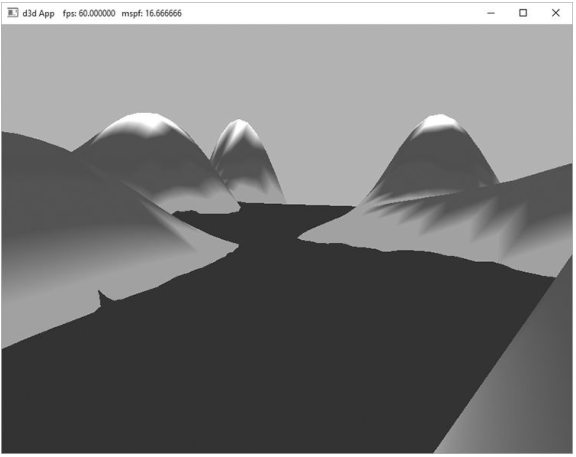
\includegraphics[width=\textwidth]{7-7}
    \centering
    \caption{“Lands and Waves”演示的屏幕截图。 因为我们还没有照明,所以很难看到波浪的形状。 按住“1”键可以在线框模式下查看场景,以更好地查看波形。}
    \label{fig:7-7}
\end{figure}

\begin{flushleft}
“漂亮”的实值(real-valued)函数$y=f(x,z)$的图是表面。 我们可以通过在$xz$平面中构建网格来近似表面,其中每个四边形由两个三角形构成,然后将函数应用于每个网格点; 见图\ref{fig:7-8}。
\end{flushleft}

\begin{figure}[h]
    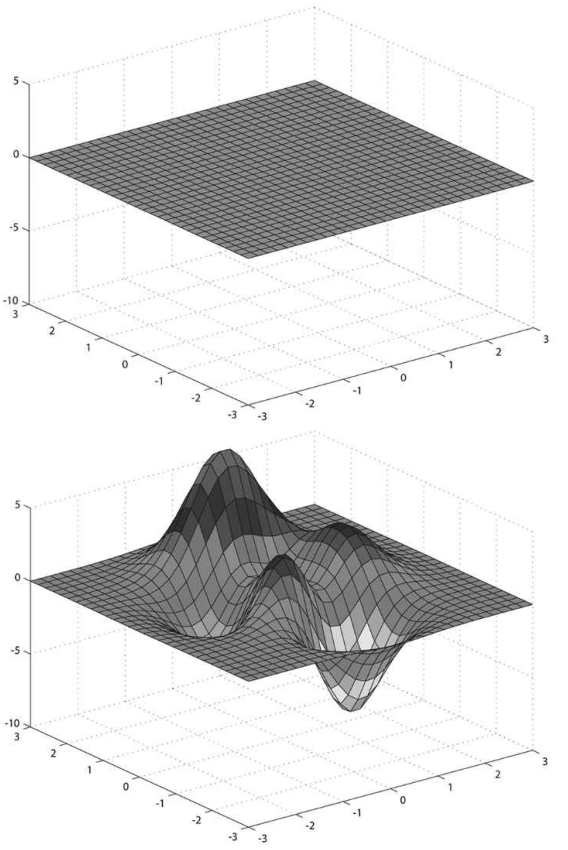
\includegraphics[width=\textwidth]{7-8}
    \centering
    \caption{(顶部)在xz平面中放置网格。(底部)对于每个网格点,应用函数f(x,z)以获得y坐标。 点(x,f(x,z),z)的图给出了曲面图。}
    \label{fig:7-8}
\end{figure}

%---- 7.7.1 ----
\subsection{创建网格顶点(Generating the Grid Vertices)}
\begin{flushleft}

\end{flushleft}



\chapter{光照(Lighting)}
\begin{flushleft}
考虑图\ref{fig:8-1}。 在左边我们有一个没有照明的球体,在右边,我们有一个点亮的球体。 正如你所看到的,左边的球体看起来很平坦——也许它根本不是一个球体,而只是一个2D圆圈! 另一方面,右侧的球体确实看起来是3D——照明和阴影有助于我们对物体的固体形状和体积的感知。 事实上,我们对世界的视觉感知取决于光线及其与材料的相互作用,因此,产生逼真场景的大部分问题都与物理上精确的照明模型有关。
\end{flushleft}

\begin{figure}[h]
    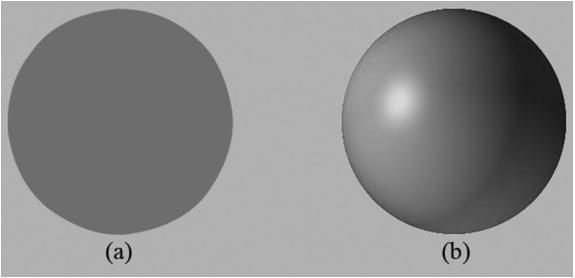
\includegraphics[width=\textwidth]{8-1}
    \centering
    \caption{(a)未点亮的球体看起来是2D。(b)点亮的球体看起来是3D。}
    \label{fig:8-1}
\end{figure}

\begin{flushleft}
当然,一般来说,模型越准确,计算成本越高; 因此,必须在现实主义和速度之间达成平衡。 例如,用于电影的3D特殊FX场景可以比游戏更复杂并且使用非常逼真的照明模型,因为电影的帧是预渲染的,因此它们可以花费数小时或数天来处理帧。 另一方面,游戏是实时应用程序,因此,帧需要以每秒至少30帧的速率绘制。\\
请注意,本书中解释和实现的照明模型很大程度上基于[Möller08]中描述的模型。\\
~\\
{\large Objectives:}
\begin{itemize}
    \item 了解灯光和材料之间的相互作用
    \item 了解局部照明和全局照明之间的差异
    \item 了解我们如何在数学上描述表面上的一个点“朝向”的方向,以便我们可以确定入射光照射到表面的角度
    \item 学习如何正确转换法向量
    \item 能够区分环境光,漫反射光和镜面光
    \item 了解如何实现定向灯,指示灯和聚光灯
    \item 通过控制衰减参数来了解如何根据深度改变光强度
\end{itemize}
\end{flushleft}

%------- 8.1 ---------------
\section{光与材质的相互作用(Light And Meterial Interaction)}
\begin{flushleft}
使用灯光时,我们不再直接指定顶点颜色; 相反,我们指定材质和灯光,然后应用光照方程式,根据光/材料相互作用计算我们的顶点颜色。 这样可以使对象更加逼真地着色(再次比较图\ref{fig:8-1}a和\ref{fig:8-1}b)。\\
可以将材质视为确定光如何与对象表面相互作用的属性。 比如表面反射和吸收的光的颜色,表面下材料的折射率,表面的光滑程度以及表面的透明度。 通过指定材质属性,我们可以模拟不同类型的真实世界表面,如木材,石材,玻璃,金属和水。\\
在我们的模型中,光源可以发出各种强度的红色,绿色和蓝色光; 通过这种方式,我们可以模拟许多浅色。 当光从光源向外传播并与物体碰撞时,一些光可能被吸收而一些光可能被反射(对于透明物体,例如玻璃,一些光线穿过介质,但我们不考虑这里的透明度)。 反射光现在沿着其新的路径行进并且可能撞击其他物体,其中一些光再次被吸收和反射。 在完全吸收之前,光线可能会撞击许多物体。 据推测,一些光线最终会进入眼睛(见图\ref{fig:8-2})并撞击视网膜上的光受体细胞(称为视锥细胞和视杆细胞)。\\
\end{flushleft}

\begin{figure}[h]
    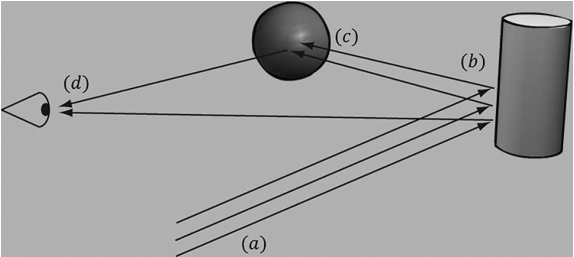
\includegraphics[width=\textwidth]{8-2}
    \centering
    \caption{(a)入射白光的通量。(b)光线照射到圆柱体上,一些光线被吸收,其他光线散射到眼睛和球体上。(c)从圆筒向球体反射的光被再次吸收或反射并进入眼睛。(d)眼睛接收入射光,确定眼睛看到的是什么。}
    \label{fig:8-2}
\end{figure}

\begin{flushleft}
根据三色理论(见[Santrock03]),视网膜含有三种光受体,每种受体对红光,绿光和蓝光敏感(有一些重叠)。 入射的RGB光根据光的强度对其相应的光接收器产生不同强度的刺激。 当光受体受到刺激(或不被刺激)时,神经冲动沿着视神经向大脑发送,大脑基于光受体的刺激在大脑中产生图像。 (当然,如果你闭上/遮住眼睛,受体细胞就不会受到任何刺激,大脑会将其记录为黑色。)\\

例如,再次考虑图\ref{fig:8-2}。假设圆柱体的材料反射75%的红光,75%的绿光,并吸收其余部分,球体反射25%的红光并吸收其余部分。还假设从光源发射纯白光。当光线照射到圆柱体上时,所有的蓝光都被吸收,只有75%的红光和绿光被反射(即,中高强度的黄色)。然后这种光被散射——其中一些光进入眼睛,一些光线向球体传播。进入眼睛的部分主要刺激红色和绿色锥形细胞达到半高度;因此,观察者将圆柱视为半亮的黄色阴影。现在,其他光线向球体射出并撞击它。球体反射25%的红光并吸收其余部分;因此,稀释的入射红光(中高强度红色)被进一步稀释并反射,并且所有进入的绿光被吸收。这剩余的红光然后进入眼睛并较低程度地刺激红锥细胞。因此,观察者将球体视为深红色。\\
我们(和大多数实时应用)在本书中采用的照明模型称为局部照明模型。 使用局部模型,每个对象独立于另一个对象被点亮,并且在光照过程中仅考虑从光源直接发射的光(即,从其他场景对象反弹以击中当前被点亮的对象的光是忽略的)。 图\ref{fig:8-3}显示了该模型的结果。
\end{flushleft}

\begin{figure}[h]
    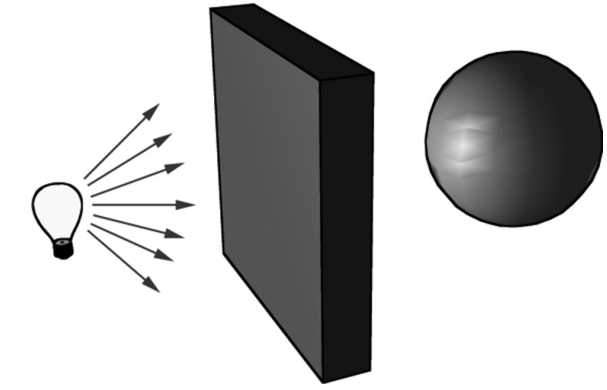
\includegraphics[width=\textwidth]{8-3}
    \centering
    \caption{在物理上,墙壁阻挡了灯泡发出的光线,并且球体位于墙壁的阴影中。 然而,在局部照明模型中,球体被照亮,好像墙壁不存在一样。}
    \label{fig:8-3}
\end{figure}

\begin{flushleft}
另一方面,全局照明通过不仅考虑从光源直接发射的光而且还考虑从场景中的其他物体反弹的间接光来模拟光物体。 这些被称为全局照明模型,因为它们在照亮对象时会考虑全局场景中的所有内容。 对于实时游戏而言,全局照明模型通常过于昂贵(但非常接近于生成逼真的场景)。 寻找近似全局照明的实时方法是一个正在进行研究的领域; 例如,参见\href{http://on-demand.gputechconf.com/gtc/2014/presentations/S4552-rt-voxel-based-global-illumination-gpus.pdf}{\textcolor{linkColor}{voxel global illumination}}。 其他流行的方法是预先计算静态对象(例如,墙壁,雕像)的间接照明,然后使用该结果来近似动态对象的间接照明(例如,移动游戏角色)。\\
\end{flushleft}

%------- 8.2 ---------------
\section{法向量(Normal Vectors)}
\begin{flushleft}
面法线(face normal)是描述多边形正面朝向的单位矢量(即,它与多边形上的所有点正交); 见图\ref{fig:8-4}a。 表面法线是与表面上的点的切平面正交的单位矢量; 见图\ref{fig:8-4}b。 观察表面法线确定表面上的点“朝向”的方向。\\
\end{flushleft}

\begin{figure}[h]
    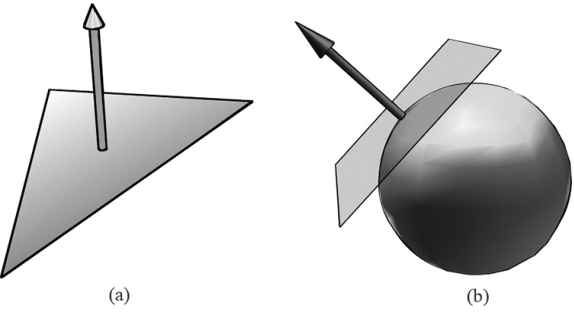
\includegraphics[width=\textwidth]{8-4}
    \centering
    \caption{(a)面部法线与面部上的所有点正交。 (b)表面法线是与表面上的点的切平面正交的矢量。}
    \label{fig:8-4}
\end{figure}

\begin{figure}[h]
    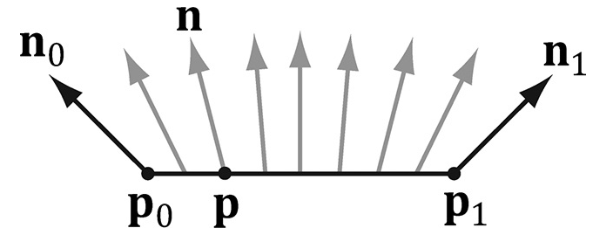
\includegraphics[width=\textwidth]{8-5}
    \centering
    \caption{顶点法线$n_{0}$和$n_{1}$在段顶点$p_{0}$和$p_{1}$处定义。 通过在顶点法线之间进行线性插值(加权平均),找到线段内部的点$p$的法向量$n$; 也就是说,$p=p_{0}+t(p_{1}-p_{0})$,其中$t$代表$p_{0}p$与$p_{0}p_{1}$的比例,则$p$的法线$n=n_{0} + t(n_{1}-n_{0})$。尽管为了简单起见我们在线段上表现了正常插值,但这个想法可以直观地应用在3D三角形上。}
    \label{fig:8-5}
\end{figure}

\begin{flushleft}
对于光照计算,我们需要在三角形网格表面上的每个点处的曲面法线,以便我们可以确定光线照射到网格曲面上的点的角度。 为了获得曲面法线,我们仅在顶点处指定曲面法线(所谓的顶点法线)。 然后,为了在三角形网格的表面上的每个点处获得近似的表面法线,这些顶点法线将在光栅化期间在三角形上插值(回忆5.10.3节并参见图\ref{fig:8-5})。\\
~\\
NOTICE: 对每个像素的法线和光照计算进行插值称为像素照明或phong照明。 一种较便宜但不太精确的方法是每个顶点进行照明计算。 然后,从顶点着色器输出每顶点光照计算的结果,并在三角形的像素上进行插值。 将像素着色器移动到顶点着色器的计算是质量方面的常见性能优化,有时视觉差异非常小,使得这种优化非常有吸引力。\\
\end{flushleft}

%------- 8.2.1 ---------------
\subsection{计算法向量(Computing Normal Vectors)}
\begin{flushleft}
为了找到三角形$p_{0}$,$p_{1}$,$p_{2}$的面法线,我们首先计算位于三角形边缘的两个向量:\\
\end{flushleft}

\begin{align*}
u=p_{1}-p_{0}\\
v=p_{2}-p_{0}
\end{align*}

\begin{flushleft}
然后,其面法向量为:\\
\end{flushleft}

\begin{align*}
n=\frac{u\times v}{||u\times v||}
\end{align*}

\begin{flushleft}
下面是一个函数,用于计算三角形三个顶点的三角形正面(5.10.2节)的面法线。\\
\end{flushleft}

\begin{lstlisting}
XMVECTOR ComputeNormal(FXMVECTOR p0, FXMVECTOR p1, FXMVECTOR p2)
{
    XMVECTOR u = p1 - p0;
    XMVECTOR v = p2 - p0;
    return XMVector3Normalize(XMVector3Cross(u,v));
}
\end{lstlisting}

\begin{figure}[h]
    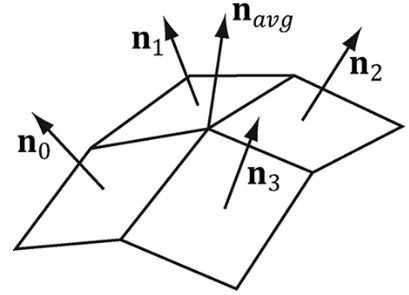
\includegraphics[width=\textwidth]{8-6}
    \centering
    \caption{中间顶点由相邻的四个多边形共享,因此我们通过平均四个多边形面法线来近似中间顶点法线。}
    \label{fig:8-6}
\end{figure}

\begin{flushleft}
对于可微分的表面,我们可以使用微积分来找到曲面上的法线。 不幸的是,三角形网格不可区分。 通常应用于三角形网格的技术称为顶点法线平均(vetex normal averaging)。 网格中的顶点法线$n$或任意顶点$v$是通过平均共享顶点$v$的网格中每个多边形的面法线来找到的。例如,在图\ref{fig:8-6}中,网格中的四个多边形因此共享顶点$v$, $v$的顶点法线由下式给出:\\
\end{flushleft}

\begin{align*}
n_{avg}=\frac{n_{0}+n_{1}+n_{2}+n_{3}}{||n_{0}+n_{1}+n_{2}+n_{3}||}
\end{align*}

\begin{flushleft}
在上面的例子中,我们不需要除以4,就像我们在典型的平均值中那样,因为我们将结果标准化。 还要注意,可以构建更复杂的平均方案; 例如,可以使用加权平均值,其中权重由多边形的面积确定(例如,具有较大区域的多边形比具有较小区域的多边形具有更多权重)。\\
以下伪代码显示了如何在给定三角形网格的顶点和索引列表的情况下实现此平均:\\
\end{flushleft}

\begin{lstlisting}
// Input:
// 1. An array of vertices (mVertices). Each vertex has a
// position component (pos) and a normal component (normal).
// 2. An array of indices (mIndices).
// For each triangle in the mesh:
for(UINT i = 0; i < mNumTriangles; ++i)
{
    // indices of the ith triangle
    UINT i0 = mIndices[i*3+0];
    UINT i1 = mIndices[i*3+1];
    UINT i2 = mIndices[i*3+2];

    // vertices of ith triangle
    Vertex v0 = mVertices[i0];
    Vertex v1 = mVertices[i1];
    Vertex v2 = mVertices[i2];

    // compute face normal
    Vector3 e0 = v1.pos - v0.pos;
    Vector3 e1 = v2.pos - v0.pos;
    Vector3 faceNormal = Cross(e0, e1);

    // This triangle shares the following three vertices,
    // so add this face normal into the average of these
    // vertex normals.
    mVertices[i0].normal += faceNormal;
    mVertices[i1].normal += faceNormal;
    mVertices[i2].normal += faceNormal;
}
// For each vertex v, we have summed the face normals of all
// the triangles that share v, so now we just need to normalize.
for(UINT i = 0; i < mNumVertices; ++i)
    mVertices[i].normal = Normalize(&mVertices[i].normal));
\end{lstlisting}

%------- 8.2.2 ---------------
\subsection{转换法向量(Transforming Normal Vectors)}
\begin{flushleft}
考虑图\ref{fig:8-7}a,其中我们具有与法向量$n$正交的切向量$u=v_{1}-v_{0}$。 如果我们应用非均匀缩放变换$A$,我们从图\ref{fig:8-7}b中看到,变换的切向量$uA=v_{1}A-v_{0}A$不与变换的法向量$nA$保持正交。
\end{flushleft}

\begin{figure}
\begin{subfigure}{1\textwidth}
  \centering
  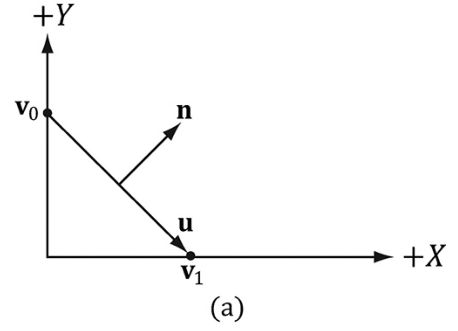
\includegraphics[width=1\linewidth]{8-7-a}
\end{subfigure}
\begin{subfigure}{1\textwidth}
  \centering
  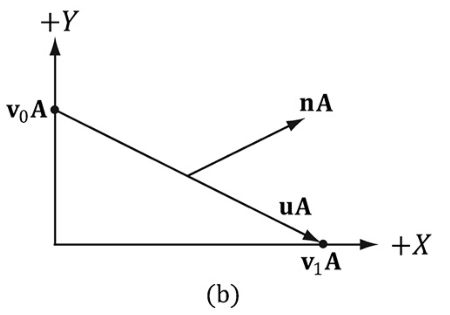
\includegraphics[width=1\linewidth]{8-7-b}
\end{subfigure}
\begin{subfigure}{1\textwidth}
  \centering
  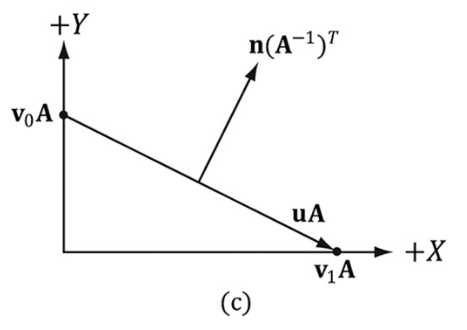
\includegraphics[width=1\linewidth]{8-7-c}
\end{subfigure}
\caption{(a)转变前的表面法线。(b)在x轴上缩放2个单位后,法线不再与表面正交。 (c)通过缩放变换的逆转置正确地变换的表面法线。}
\label{fig:8-7}
\end{figure}

\begin{flushleft}
所以我们的问题是:给定转换矩阵$A$转换点和向量(非正态),我们想找到一个转换矩阵$B$,使得转换的切线向量与转换的法向量正交(即 $uA\cdot nB = 0$)。 要做到这一点,首先从我们知道的东西开始:我们知道法向量$n$与切向量$u$正交:\\
\end{flushleft}

\begin{tabular}{|p{5em}|p{35em}|} 
\hline
$u\cdot n=0$ & 切线向量与法向量正交\\ 
\hline
$un^{T}=0$ & 将点积重写为矩阵乘法\\ 
\hline
$u(AA^{-1})n^{T}=0$ & 插入单位矩阵$I=AA^{-1}$\\
\hline 
$(uA)(A^{-1}n^{T})=0$ & 矩阵乘法结合律\\
\hline 
$(uA)(((A^{-1}n^{T})^{T})^{T})=0$ & 矩阵转置性质:$(A^{T})^{T}=A$\\
\hline 
$(uA)((n(A^{-1})^{T})^{T})=0$ & 矩阵转置性质:$(AB^{T})^{T}=B^{T}A^{T}$\\
\hline 
$uA\cdot n(A^{-1})^{T}=0$ & 将矩阵乘法重写为点积\\ 
\hline
$uA\cdot nB=0$ & 经B转换的法向量与经A转换的法向量正交\\ 
\hline
\end{tabular}

\begin{flushleft}
因此,$B=(A^{-1})^{T}$(A的逆转置)在转换法向量时起作用,使得它们垂直于其相关的变换切线向量$uA$。\\

注意,如果矩阵是正交的(正交矩阵$(A^{T}=A^{-1})$),则$B=(A^{-1})^{T}=(A^{T})^{T}=A$; 也就是说,我们不需要计算逆转置,因为A在这种情况下完成了工作。 总之,当通过非均匀或剪切变换转换法向量时,请使用逆转置。\\
我们在 MathHelper.h 中实现了一个辅助函数来计算逆转换:\\
\end{flushleft}

\begin{lstlisting}
static XMMATRIX InverseTranspose(CXMMATRIX M)
{
    XMMATRIX A = M;
    A.r[3] = XMVectorSet(0.0f, 0.0f, 0.0f, 1.0f);
    XMVECTOR det = XMMatrixDeterminant(A);
    return XMMatrixTranspose(XMMatrixInverse(&det, A));
}
\end{lstlisting}

\begin{flushleft}
我们清除矩阵中的任何平移转换,因为我们使用逆转置来转换向量,并且转换仅适用于点。 但是,根据 3.2.1 节,我们知道为向量设置$w=0$(使用齐次坐标)可以防止向量被平移变换修改。 因此,我们不应该将矩阵中的平移归零。 问题是如果我们想要连接逆转置和不包含非均匀缩放的另一个矩阵,比如视图矩阵$(A^{-1})^{T}V$,$(A^{-1})^{T}$的第四列中的转置平移"泄漏"(leaks)到矩阵乘法运算导致错误。因此,我们将平移归零以作为预防措施以避免此错误。 正确的方法是通过以下方式转换法线:$((AV)^{-1})^{T}$。 下面是缩放和平移矩阵的示例,以及第四列不是$[0,0,0,1]^{T}$的逆转置看起来是什么样的:\\
\end{flushleft}

\begin{align*}
A&=
\begin{bmatrix}
1 & 0 & 0 & 0\\
0 & 0.5 & 0 & 0\\
0 & 0 & 0.5 & 0\\
1 & 1 & 1 & 1
\end{bmatrix}\\
(A^{-1})^{T}&=
\begin{bmatrix}
1 & 0 & 0 & -1\\
0 & 2 & 0 & -2\\
0 & 0 & 2 & -2\\
0 & 0 & 0 & 1
\end{bmatrix}
\end{align*}

\begin{flushleft}
NOTICE: 即使使用逆转置变换,法向量也可能失去单位长度; 因此,它们可能需要在转换后重新规范化。
\end{flushleft}

%------- 8.3 ---------------
\section{照明中的重要向量(Important Vectors In Lighting)}
\begin{flushleft}
在本节中,我们总结了一些与照明有关的重要向量。参考图\ref{fig:8-8},$E$是眼睛位置,我们正在考虑眼睛沿着由单位向量$v$定义的位置线看到的点$p$。在点$p$ 处,表面具有法向量$n$,并且该点被一个入射方向$I$的光线击中。光向量$L$是朝向撞击表面点的光线的相反方向的单位矢量。虽然使用光传播方向可能更直观,但对于光照计算,我们使用光向量$L$;特别地,为了计算朗伯余弦定律(Lambert’s Cosine Law),向量$L$用于计算$L\cdot n=cos\Theta_{i}$,其中$\Theta_{i}$是$L$和$n$之间的角度。反射向量$r$是关于表面法线$n$的入射光向量的反射。视图向量(或眼睛向量)$v$=标准化$(E-p)$是从表面点$p$到眼点$E$的单位向量,其定义从眼睛到被观察表面上的点的位置线。有时我们需要使用矢量$-v$,它是从眼睛到表面上我们正在计算光照的点的单位向量。\\
\end{flushleft}

\begin{figure}[h]
    \label{fig:8-8}
    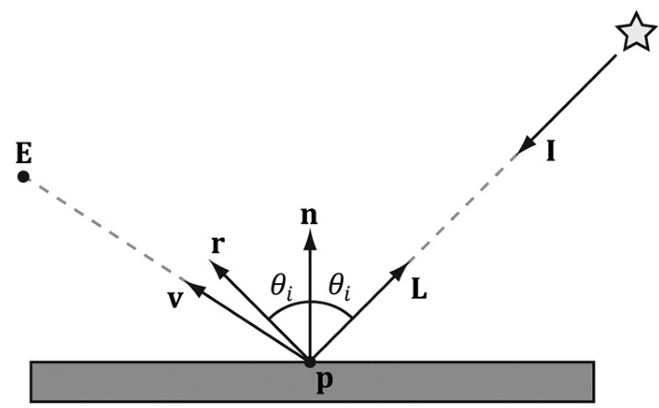
\includegraphics[width=\textwidth]{8-8}
    \centering
    \caption{光照计算中涉及到的重要向量}
\end{figure}

\begin{flushleft}
反射向量由下式给出:$r=I-2(n\cdot I)n$; 见图\ref{fig:8-9}。 (假设$n$是单位向量。)但是,我们实际上可以使用HLSL内部反射函数在着色器程序中为我们计算$r$。
\end{flushleft}

\begin{figure}[h]
    \label{fig:8-9}
    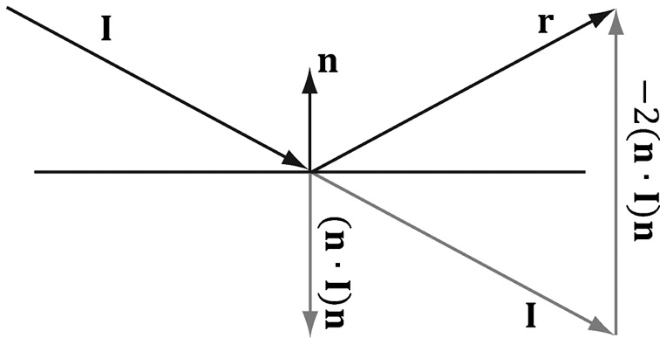
\includegraphics[width=\textwidth]{8-9}
    \centering
    \caption{反射几何}
\end{figure}

%------- 8.4 ---------------
\section{朗伯余弦定律(Lambert’s Cosine Law)}
\begin{flushleft}
我们可以将光视为在某个方向上穿过空间的光子集合。每个光子携带一些(光)能量。 每秒发射的(光)能量的量称为辐射通量。 每个区域的辐射通量密度(称为辐照度)很重要,因为这将决定表面上的区域接收多少光(它对眼睛看起来有多亮)。 粗略说,我们可以将辐照度视为撞击表面上的区域的光量,或者通过空间中的假想区域的光量。\\

正面撞击表面的光(即,光向量$L$等于法线向量$n$)比以一定角度掠过表面的光更强烈。考虑具有横截面积$A_{1}$的小光束,其中辐射通量$P$穿过它。 如果我们将这个光束瞄准正面(图\ref{fig:8-10}a),则光束照射到表面上的区域$A_{1}$,$A_{1}$处的辐照度为$E_{1}=P/A_{1}$。 现在假设我们旋转光束使其以一定角度撞击表面(图\ref{fig:8-10}b),然后光束覆盖较大的区域$A_{2}$,并且照射该区域的辐照度为$E_{2}=P/A_{2}$。 通过三角函数,$A_{1}$和$A_{2}$通过以下方式关联:\\
\end{flushleft}

\begin{align*}
cos\Theta = \frac{A_{1}}{A_{2}}\Rightarrow \frac{1}{A_{2}}=\frac{cos\Theta}{A_{1}}
\end{align*}

\begin{flushleft}
所以,\\
\end{flushleft}

\begin{align*}
E_{2}=\frac{P}{A_{2}}=\frac{P}{A_{1}}cos\Theta=E_{1}cos\Theta=E_{1}(n\cdot L)
\end{align*}

\begin{figure}[h]
    \label{fig:8-10}
    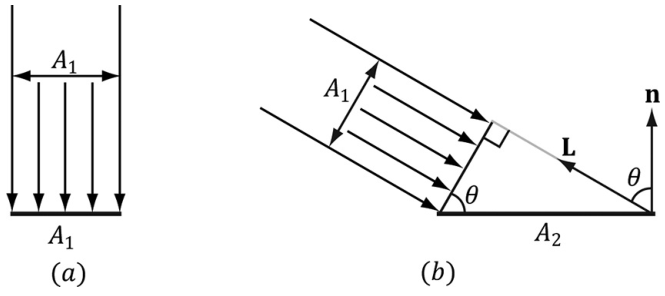
\includegraphics[width=\textwidth]{8-10}
    \centering
    \caption{(a)横截面积为$A_{1}$的光束正面撞击表面。(b)具有横截面面积$A_{1}$的光束以一定角度撞击表面以覆盖表面上的较大区域$A_{2}$,从而将光能扩散到更大的区域上,从而使光看起来“更暗”。}
\end{figure}

\begin{flushleft}
换句话说,辐照度打击区域$A_{2}$等于垂直于被$n\cdot L=cos\Theta$缩放变换的光方向的区域$A_{1}$处的辐照度。 这被称为兰伯特的余弦定律。 为了处理光线照射到背面(导致点积为负)的情况,我们用最大函数限制结果:\\
\end{flushleft}

\begin{align*}
f(\Theta)=max(cos\Theta,0)=max(L\cdot n, 0)
\end{align*}

\begin{flushleft}
图\ref{fig:8-11}显示了$f(\Theta)$的曲线图,以观察 0.0 到 1.0(即0%到100%)的强度如何随θ变化。
\end{flushleft}

\begin{figure}[h]
    \label{fig:8-11}
    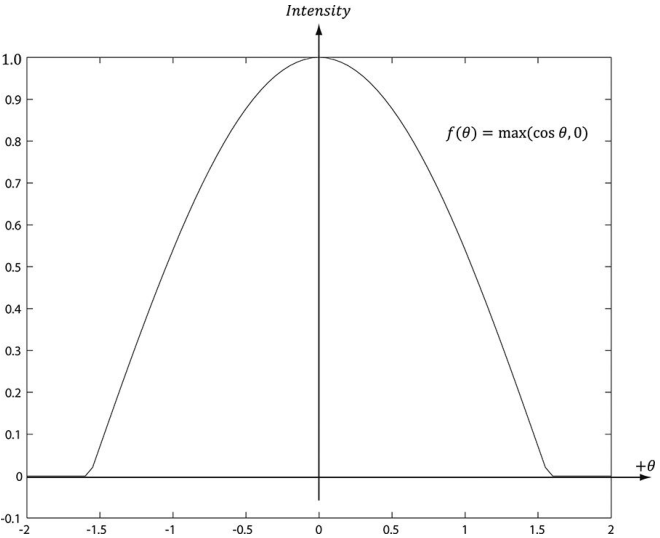
\includegraphics[width=\textwidth]{8-11}
    \centering
    \caption{对于$-2\leq \Theta \leq 2$,函数$f(\Theta)=max(cos\Theta,0)=max(L\cdot n, 0)$的曲线图。注意$\pi /2 \approx 1.57$。}
\end{figure}

%------- 8.5 ---------------
\section{漫射照明(Diffuse Lighting)}
\begin{flushleft}
考虑不透明物体的表面,如图\ref{fig:8-12}所示。当光线照射到表面上的某个点时,一些光线会进入物体内部并与表面附近的物质相互作用。光线会在内部反射,其中一些会被吸收,剩下的部分会向各个方向散射出来;这称为漫反射。为简化起见,我们假设光线在光线进入的同一点散射出来。吸收和散射的量取决于材料;例如,木材,泥土,砖块,瓷砖和灰泥会不同地吸收/散射光线(这就是材料看起来不同的原因)。我们对这种光/材料相互作用近似建模,规定光在表面上方的所有方向上均匀散射;因此,无论视点(眼睛位置)如何,反射光都会到达眼睛。因此,我们不需要考虑该视点(即,漫射照明计算是视点无关的),并且无论视点如何,表面上的点的颜色总是看起来相同。\\
\end{flushleft}

\begin{figure}[h]
    \label{fig:8-12}
    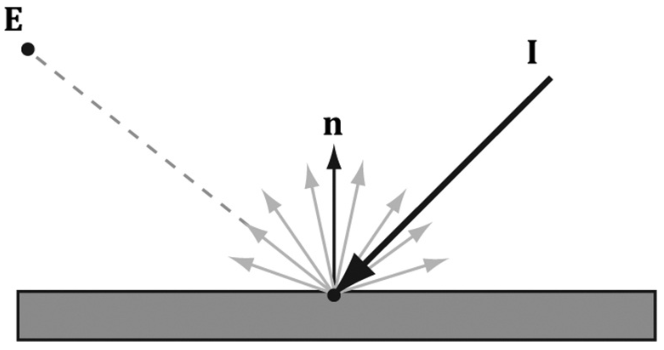
\includegraphics[width=\textwidth]{8-12}
    \centering
    \caption{当撞击漫射表面时,入射光在每个方向上均匀地散射。 这个想法是光进入介质的内部并在表面下散射。 一些光将被吸收,剩余的光会从表面散射回来。 因为很难对这种次表面散射进行建模,所以我们假设重新发射的光在光进入的点附近在表面上方的所有方向上均匀地散射出来。}
\end{figure}

\begin{flushleft}
我们将漫射照明的计算分为两部分。 对于第一部分,我们指定浅色和漫反射色。 漫反射率指定了由于漫反射而表面反射的入射光量(通过节能,未反射的量被材料吸收)。 这是通过分量色彩乘法处理的(因为光可以着色)。 例如,假设表面上的某些点反射50%的入射红光,100%的绿光和75%的蓝光,并且入射光的颜色是80%强度的白光。 也就是说,入射光量由$B_{L}=(0.8,0.8,0.8)$给出,漫反射率由$m_{d}=(0.5,1.0,0.75)$ 给出; 那么从该点反射的光量由下式给出:\\
\end{flushleft}

\begin{align*}
c_{d}=B_{L}\bigotimes m_{d}=(0.8,0.8,0.8)\bigotimes (0.5,1.0,0.75)=(0.4,0.8,0.6)
\end{align*}

\begin{flushleft}
请注意,漫反射率反射率分量必须在0.0到1.0的范围内,以便它们描述反射光的分数。\\
但是,上述公式并不完全正确。 我们仍然需要引入Lambert的余弦定律(它根据表面法线和光向量之间的角度控制表面接收的原始光的多少)。 设$B_{L}$表示入射光量,$m_{d}$ 是漫反射率颜色,$L$是光向量,$n$是表面法线。 然后,一个点反射的漫射光量由下式给出:\\
\end{flushleft}

\begin{align*}\tag{eq.8.1}\label{eq.8.1}
c_{d}=max(L\cdot n, 0)\cdot B_{L}\bigotimes m_{d}
\end{align*}

%------- 8.6 ---------------
\section{环境照明(Ambient Lighting)}
\begin{flushleft}
如前所述,我们的照明模型没有考虑从场景中的其他物体反弹的间接光。 然而,我们在现实世界中看到的很多光是间接的。 例如,连接到房间的走廊可能不在房间的直接线路中,房间内有光源,但是灯光从房间的墙壁反弹,有些可能会进入走廊,从而使其变亮一点点。 作为第二个例子,假设我们坐在桌子上有茶壶的房间里,房间里有一个光源。 只有茶壶的一侧位于光源的直线上; 然而,茶壶的背面不会是完全黑色的。 这是因为一些光线从房间的墙壁或其他物体上散开,最终撞击茶壶的背面。\\
为了解释这种间接光,我们在照明方程中引入了一个环境术语:\\
\end{flushleft}

\begin{align*}\tag{eq.8.2}\label{eq.8.2}
c_{a}=A_{L}\bigotimes m_{d}
\end{align*}

\begin{flushleft}
颜色$A_{L}$表示表面接收的间接(环境)光的总量,与从光源发出的光不同,这是由于当光从其他表面反弹时发生的吸收。 漫反射率$m_{d}$表示由于漫反射而表面反射的入射光量。 我们使用相同的值来指定表面反射的入射环境光量; 也就是说,对于环境照明,我们正在模拟间接(环境)光的漫反射。 所有环境光都会使物体均匀亮一点 - 根本没有真正的物理计算。 这个想法是,间接光在场景周围散射和反射很多次,以至于它在每个方向上均匀地撞击物体。
\end{flushleft}

%------- 8.7 ---------------
\section{高光照明(Specular Lighting)}
\begin{flushleft}
我们使用漫射照明来模拟漫反射,其中光进入介质,反射,一些光被吸收,剩余的光在每个方向上从介质中散射出来。 由于菲涅耳效应(Fresnel effect),发生了第二种反射,这是一种物理现象。 当光线到达具有不同折射率的两种介质之间的界面时,一些光被反射,剩余的光被折射(见图\ref{fig:8-13})。 折射率是介质的物理性质,其是真空中的光速与给定介质中的光速之比。 我们将这种光反射过程称为镜面反射,将反射光称为镜面反射光。 镜面光如图\ref{fig:8-14}a所示。
\end{flushleft}

\begin{figure}[h]
    \label{fig:8-13}
    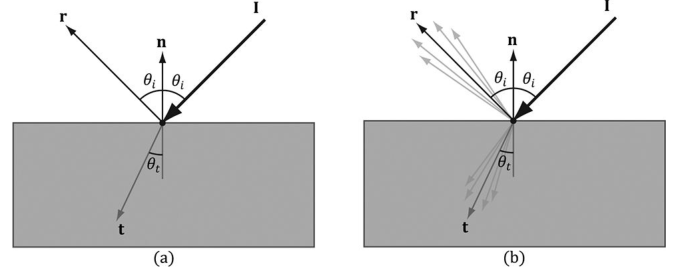
\includegraphics[width=\textwidth]{8-13}
    \centering
    \caption{(a)对于具有法向量$n$的完全平坦的镜子的菲涅耳效应(Frenel eefct)。 入射光$I$被分开,其中一些光在反射方向$r$上反射,并且剩余的光在折射方向$t$上折射到介质中。 所有这些向量都在同一平面上。 反射向量和法线之间的角度总是$θ_{i}$,这与光向量$L=-I$和法线$n$之间的角度相同。 折射向量和$-n$之间的角度$θ_{t}$取决于两种介质之间的折射率,并由斯涅尔定律(Snell's Law)表示。 (b)大多数物体不是完全平坦的镜子,但具有微观粗糙度。 这导致反射和折射的光在反射和折射矢量周围扩散。}
\end{figure}

\begin{flushleft}
如果折射的向量离开介质(从另一侧)并进入眼睛,则该物体看起来是透明的。 也就是说,光线穿过透明物体。 实时图形通常使用alpha混合或后期处理效果来近似透明对象的折射,我们将在本书后面解释。 目前,我们只考虑不透明的对象。\\
对于不透明物体,折射光进入介质并经历漫反射。 因此我们可以从图\ref{fig:8-14}b中看到,对于不透明物体,从表面反射并使其进入眼睛的光量是身体反射(漫射)光和镜面反射的组合。 与漫射光相比,镜面光可能不会进入眼睛,因为它反射在特定方向; 也就是说,镜面反射计算是视点相关的。 这意味着当眼睛在场景周围移动时,它接收的镜面光量将发生变化。\\
\end{flushleft}

\begin{figure}[h]
    \label{fig:8-14}
    \includegraphics[width=\textwidth]{8-14}
    \centering
    \caption{(a)粗糙表面的镜面光围绕反射向量$r$扩散。 (b)使其进入眼睛的反射光是镜面反射和漫反射的组合。}
\end{figure}

%------- 8.7.1 ---------------
\subsection{菲涅耳效应(Fresnel Effect)}
\begin{flushleft}
让我们考虑具有法向量$n$的平坦表面,该向量将具有不同折射率的两种介质分开。 由于表面处的折射率不连续,当入射光照射到表面时,一些反射离开表面,一些折射到表面(见图\ref{fig:8-13})。 菲涅耳方程在数学上描述了被反射的入射光的百分比,$0\leq R_{F} \leq 1$。通过能量守恒,如果$R_{F}$是反射光的量,则$(1-R_{F})$是折射光的量。 值$R_{F}$是 RGB 向量,因为反射量取决于光的颜色。\\
反射的光量取决于介质(某些材料将比其他材料更具反射性)以及法向量$n$和光向量$L$之间的角度$\Theta_{i}$。由于它们的复杂性,完整的菲涅耳方程通常不用于实时渲染; 相反,使用 Schlick 近似:\\
\end{flushleft}

\begin{align*}
R_{F}(\Theta_{i})=R_{F}(0^{\circ})+(1-R_{F}(0^{\circ}))(1-cos\Theta_{i})^{5} 
\end{align*}

\begin{flushleft}
$R_{F}(0^{\circ})$是介质的特性; 以下是常见材料的一些值[Möller08]:\\
\end{flushleft}

\begin{tabular}{|p{5em}|p{35em}|} 
\hline
介质 & $R_{F}(0^{\circ})$\\ 
\hline
水 & $(0.02,0.02,0.02)$\\ 
\hline
玻璃 & $(0.08,0.08,0.08)$\\ 
\hline
塑料 & $(0.05,0.05,0.05)$\\ 
\hline
金 & $(1.0,0.71,0.29)$\\ 
\hline
银 & $(0.95,0.93,0.88)$\\ 
\hline
铜 & $(0.95,0.64,0.54)$\\ 
\hline
\end{tabular}

\begin{flushleft}
图\ref{fig:8-15}显示了几个不同$R_{F}(0^{\circ})$的 Schlick 近似图。观察的关键是反射量随着$\Theta_{i}\rightarrow 90^{\circ}$的增加而增加。让我们看一个现实世界的例子。考虑图\ref{fig:8-16}。假设我们站在一个相对清澈的水的平静池塘深处几英尺深。如果我们向下看,我们大多看到池塘底部的沙子和岩石。这是因为从环境反射到我们眼睛中的光形成了接近$0.0^{\circ}$的小角度$\Theta_{i}$;因此,反射量低,并且因为节能,折射量高。另一方面,如果我们望向地平线,我们将看到池塘水中的强烈反射。这是因为从进入我们眼睛的环境下来的光形成接近$90.0^{\circ}$的角度$\Theta_{i}$,从而增加了反射量。此行为通常称为菲涅耳效应。简要总结菲涅耳效应:反射光的量取决于材料$R_{F}(0^{\circ})$和法向量与光向量之间的角度。\\
\end{flushleft}

\begin{figure}[h]
    \label{fig:8-15}
    \includegraphics[width=\textwidth]{8-15}
    \centering
    \caption{针对不同材料绘制的Schlick近似值:水,红宝石和铁。}
\end{figure}

\begin{figure}[h]
    \label{fig:8-16}
    \includegraphics[width=\textwidth]{8-16}
    \centering
    \caption{(a):俯视池塘,反射低,折射高,因为$L$和$n$之间的角度很小。 (b)看向地平线,反射高,折射低,因为$L$和$n$之间的角度接近$90^{\circ}$。}
\end{figure}

\begin{flushleft}
金属吸收透射光[Möller08],这意味着它们不会有人体反射。 然而,金属看起来不是黑色,因为它们具有高$R_{F}(0^{\circ})$值,这意味着即使在$0^{\circ}$附近的小入射角下它们也能反射相当数量的镜面反射光。\\
\end{flushleft}
\clearpage

%------- 8.7.2 ---------------
\subsection{粗糙度(Roughness)}
\begin{flushleft}
现实世界中的反光物体往往不是完美的镜子。 即使物体的表面看起来是扁平的,在微观层面我们也可以认为它具有粗糙度。 参见图\ref{fig:8-17},我们可以认为一个完美的镜子没有粗糙度,它的微法线都与宏观法线的方向相同。 随着粗糙度的增加,微法线的方向偏离宏观法线,导致反射光扩散到镜面波瓣。
\end{flushleft}

\begin{figure}[h]
    \label{fig:8-17}
    \includegraphics[width=\textwidth]{8-17}
    \centering
    \caption{(a)黑色水平条表示小表面元素的放大。 在微观层面,该区域具有许多微观法线,由于微观水平的粗糙度而瞄准不同的方向。 表面越光滑,微法线与宏观法线的平均值越大; 表面越粗糙,微法线就越偏离宏观法线。(b)这种粗糙度导致镜面反射光扩散。 镜面反射的形状称为镜面反射。 通常,镜面凸角的形状可以根据被建模的表面材料的类型而变化。}
\end{figure}

\begin{flushleft}
为了在数学上模拟粗糙度,我们采用了微平面模型,我们将微观表面建模为一组称为微平面的微小扁平元素; 微法线是微平面的法线。 对于给定的视图$v$和光向量$L$,我们想要知道将$L$反射为$v$的微平面的分数(faction); 换句话说,具有法线$h=$标准化$(L + v)$的微平面的分数(faction); 见图\ref{fig:8-18}。 这将告诉我们有多少光线从镜面反射到眼睛中——将$L$反射到$v$中的微透镜越多,眼睛看到的镜面反射光越亮。
\end{flushleft}

\begin{figure}[h]
    \label{fig:8-18}
    \includegraphics[width=\textwidth]{8-18}
    \centering
    \caption{具有法线$h$的微平面将$L$反射为$v$。}
\end{figure}

\begin{flushleft}
向量$h$被称为中间向量,因为它位于$L$和$v$之间的中间。此外,我们还介绍中间向量$h$和宏观法线$n$之间的角度$\Theta h$。\\

我们定义归一化分布函数$\rho(\Theta_{h})\epsilon [0,1]$来表示具有法线$h$的微平面的分数,其与宏观法线$n$形成角度$\Theta h$。 直观地,我们期望当$\Theta h=0^{\circ}$时$\rho(\Theta_{h})$达到其最大值。 也就是说,我们预计微平面法线偏向宏观法线,并且随着$\Theta h$增加(当$h$偏离微法线$n$时),法线$h$的微平面的比例将减小。 一个流行的可控函数模型$\rho(\Theta_{h})$符合刚才讨论的期望:\\
\end{flushleft}

\begin{align*}
\rho(\Theta_{h})&=cos^{m}(\Theta_{h})\\
&=cos^{m}(n\cdot h)
\end{align*}

\begin{flushleft}
注意,$cos(\Theta h)=(n\cdot h)$提供了向量和单位长度。 图\ref{fig:8-19}显示了各种$m$的$\rho(\Theta_{h})=cos_{h}(\Theta_{h})$。 这里$m$控制粗糙度,代表具有法线$h$的微平面的分数,与宏观法线$n$形成角度$\Theta_{h}$。 随着$m$减小,表面变得更粗糙,并且微平面法线越来越偏离宏观法线。 随着$m$增加,表面变得更平滑,并且微平面法线越来越收敛于宏观法线。
\end{flushleft}

\begin{figure}[h]
    \label{fig:8-19}
    \includegraphics[width=\textwidth]{8-19}
    \centering
    \caption{具有法线$h$的微平面将$L$反射为$v$。}
\end{figure}

\begin{flushleft}
我们可以将$\rho(\Theta_{h})$与归一化因子结合起来,以获得一个基于粗糙度模拟光的镜面反射量的新函数:\\
\end{flushleft}

\begin{align*}
S(\Theta_{h})&=\frac{m+8}{8}cos^{m}(\Theta_{h})\\
&=\frac{m+8}{8}(n\cdot h)^{m}
\end{align*}

\begin{flushleft}
图\ref{fig:8-20}显示了该函数的各种$m$。 像以前一样,$m$控制粗糙度,但我们增加了$\frac{m+8}{8}$归一化因子,以便保存光能; 它基本上控制了图\ref{fig:8-20}中曲线的高度,因此当镜面波瓣变宽或变窄时,整体光能得以保存。 对于较小的$m$,表面较粗糙,镜面波瓣随着光能量的扩散而变宽; 因此,我们预计,由于能量已经分散,镜面高光会变暗。 另一方面,对于更大的$m$,表面更光滑并且镜面波瓣更窄; 因此,我们预计,由于能量集中,镜面高光更加明亮。 几何上,$m$控制镜面波瓣的扩散。 要模拟光滑的表面(如抛光金属),您将使用较大的$m$,而对于较粗糙的表面,您将使用较小的$m$。
\end{flushleft}

\begin{figure}[h]
    \label{fig:8-20}
    \includegraphics[width=\textwidth]{8-20}
    \centering
    \caption{由粗糙度模拟光的镜面反射的函数。}
\end{figure}

\begin{flushleft}
总结本节,让我们结合菲涅耳反射和表面粗糙度。 我们正在尝试计算反射到视图方向$v$的光量(见图\ref{fig:8-18})。 回想一下,具有法线$h$的微平面将光反射到$v$中。令$\alpha_{h}$是光向量和半向量$h$之间的角度,然后$R_{F}(\alpha_{h})$告诉我们由于菲涅耳效应而将$h$反射到$v$中的光量。 由于菲涅耳效应引起的反射光$R_{F}(\alpha_{h})$的量乘以由粗糙度$S(\Theta_{h})$引起的反射光量,得到镜面反射光的量:$(max(L\cdot n,0)\cdot B_{L})$表示撞击我们正在照射的表面点的入射光的量,然后由于粗糙度和菲涅耳效应而镜面反射到眼睛中的$(max(L\cdot n,0)\cdot B_{L})$的分数由下式给出:\\
\end{flushleft}

\begin{align*}\tag{eq.8.3}\label{eq.8.3}
c_{s}=max(L\cdot n, 0)\cdot B_{L}\bigotimes R_{F}(\alpha_{h})\frac{m+8}{8}(n\cdot h)^{m}
\end{align*}

\begin{flushleft}
观察到如果$L\cdot n\leq 0$,则光线照射到我们正在计算的表面背面;因此前侧表面不接收光。
\end{flushleft}

%------- 8.8 ---------------
\section{照明模型回顾(Lighting Model Recap)}
\begin{flushleft}
将所有物质组合在一起,从表面反射的总光量是环境光反射率,漫反射光反射率和镜面反射光的总和:\\
\end{flushleft}

\begin{itemize}
  \item 1.环境光$c_{a}$:模拟由于间接光线而从表面反射的光量。
  \item 2.漫射光$c_{d}$:模拟进入介质内部的光线,散射在表面下方,其中一些光线被吸收,剩余的光线从表面散射回来。 因为很难对这种次表面散射进行建模,所以我们假设重新发射的光在光进入的点附近在表面上方的所有方向上均匀地散射出来。
  \item 3.镜面光$c_{s}$:模拟由于菲涅耳效应和表面粗糙度而从表面反射的光。\\
  这导致我们的着色器在本书中实现的照明方程:\\
  \begin{align*}\tag{eq.8.4}\label{eq.8.4}
  LitColor&=c_{a}+c_{d}+c{s}\\
  &=A_{L}\bigotimes m_{d}+max(L\cdot n, 0)\cdot B_{L}\bigotimes (m_{d}+R_{F}(\alpha_{h})\frac{m+8}{8}(n\cdot h)^{m})
  \end{align*}
\end{itemize}

\begin{flushleft}
假设该等式中的所有向量都是单位长度。\\
\end{flushleft}

\begin{itemize}
  \item 1.$L$:光向量瞄准光源。
  \item 2.$n$:平面法向量。
  \item 3.$h$:中间向量位于光向量和视图向量之间(从点亮的表面点到眼点的向量)。
  \item 4.$A_{L}$:表示进入的环境光的数量。
  \item 5.$B_{L}$:表示进入的直射光量。
  \item 6.$m_{d}$:指定由于漫反射而表面反射的入射光的量。
  \item 7.$L\cdot n$:朗伯余弦定理。
  \item 8.$\alpha_{h}$:半向量$h$和光向量$L$之间的角度。
  \item 9.$R_{F}(\alpha_{h})$:表示由于菲涅耳效应而进入眼睛的$h$反射光量。
  \item 10.$m$:控制表面粗糙度。
  \item 11.$(n\cdot h)_{h}$:表示具有法线$h$的微平面的分数,其与宏观法线$n$形成角度$θ_{h}$。
  \item 12.$\frac{m+8}{8}$:在镜面反射中模拟能量守恒的归一化因子。
\end{itemize}

\begin{flushleft}
图\ref{fig:8-21}显示了三种光模型作用在一起的样子。\\
\end{flushleft}

\begin{figure}[h]
    \label{fig:8-21}
    \includegraphics[width=\textwidth]{8-21}
    \centering
    \caption{(a)仅用环境光着色的球体,均匀地照亮它。(b)环境光和漫射照明相结合。 由于朗伯余弦定律,现在从明亮到黑暗平稳过渡。(c)环境光,漫反射光和镜面光。 镜面反射照明产生镜面反射。}
\end{figure}

\begin{flushleft}
NOTICE: 公式8.4是一种常见且流行的照明方程,但它只是一个模型。还有其他照明模型。
\end{flushleft}

%------- 8.9 ---------------
\section{实现材质(Implementing Materials)}
\begin{flushleft}
材质数据结构如下,其定义在 d3dUtil.h 中:\\
\end{flushleft}

\begin{lstlisting}
// Simple struct to represent a material for our demos.  
// A production 3D engine would likely create a class 
// hierarchy of Materials.
struct Material
{
    // Unique material name for lookup.
    std::string Name;

    // Index into constant buffer corresponding to this material.
    int MatCBIndex = -1;

    // Index into SRV heap for diffuse texture.
    int DiffuseSrvHeapIndex = -1;

    // Index into SRV heap for normal texture.
    int NormalSrvHeapIndex = -1;

    // Dirty flag indicating the material has changed and
    // we need to update the constant buffer.
    // Because we have a material constant buffer for each 
    // FrameResource, we have to apply the
    // update to each FrameResource.  Thus, when we modify 
    // a material we should set 
    // NumFramesDirty = gNumFrameResources so that each frame 
    // resource gets the update.
    int NumFramesDirty = gNumFrameResources;

    // Material constant buffer data used for shading.
    DirectX::XMFLOAT4 DiffuseAlbedo = { 1.0f, 1.0f, 1.0f, 1.0f };
    DirectX::XMFLOAT3 FresnelR0 = { 0.01f, 0.01f, 0.01f };
    float Roughness = .25f;
    DirectX::XMFLOAT4X4 MatTransform = MathHelper::Identity4x4();
};
\end{lstlisting}

\begin{flushleft}
对真实世界的材料进行建模需要结合为DiffuseAlbedo和FresnelR0设置实际值,以及一些艺术调整。 例如,金属导体吸收进入金属内部的折射光[Möller08],这意味着金属不会有漫反射(即,DiffuseAlbedo将为零)。 然而,为了补偿我们没有进行100%的光照物理模拟,设置不为零的低DiffuseAlbedo值可以提供更好的艺术效果。 重点是:我们将尝试使用物理上真实的材料值,也可以随意调整我们想要的值以求更好的效果(艺术的角度)。\\
在我们的材料数据结构中,粗糙度在$[0,1]$范围内的标准化浮点值中取值。 粗糙度为 0 表示表面非常光滑,粗糙度为 1 表示物理上可能的最粗糙表面。 标准化范围使得更容易编写粗糙度并比较不同材料之间的粗糙度。 例如,粗糙度为0.6的材料的粗糙度是粗糙度为0.3的材料的两倍。 在着色器代码中,我们将使用粗糙度来导出公式\ref{eq.8.4}中使用的指数$m$。 请注意,根据我们对粗糙度的定义,表面的光泽度(shininess)只是粗糙度(roughness)的倒数:$shininess=1-roughness \epsilon [0,1]$。\\

现在的问题是我们应该在什么样的粒度上指定材料值?材料值可能在表面上变化; 也就是说,表面上的不同点可能具有不同的材料值。 例如,考虑如图\ref{fig:8-22}所示的汽车模型,其中框架,窗户,灯光和轮胎以不同方式反射和吸收光线,因此材料值需要在汽车表面上变化。
\end{flushleft}

\begin{figure}[h]
    \label{fig:8-22}
    \includegraphics[width=\textwidth]{8-22}
    \centering
    \caption{汽车网格划分为五个材料属性组。}
\end{figure}

\begin{flushleft}
要实现此变化,一种解决方案可能是在每个顶点的基础上指定材质值。 然后,这些每个顶点材质将在光栅化期间在三角形上进行插值,为三角形网格表面上的每个点提供材质值。 然而,正如我们在第7章的“Hills”演示中看到的那样,每个顶点颜色仍然太粗糙,无法逼真地模拟精细细节。 此外,每个顶点颜色会向我们的顶点结构添加额外的数据,我们需要使用工具来绘制每个顶点颜色。 相反,流行的解决方案是使用纹理映射,它必须等到下一章。 对于本章,我们允许在绘制调用频率上进行材料更改。 为此,我们定义每个唯一材料的属性并将它们放在一个表中:\\
\end{flushleft}

\begin{lstlisting}
std::unordered_map<std::string, 
    std::unique_ptr<Material>> mMaterials;
void LitWavesApp::BuildMaterials()
{
    auto grass = std::make_unique<Material>();
    grass->Name = “grass”;
    grass->MatCBIndex = 0;
    grass->DiffuseAlbedo = XMFLOAT4(0.2f, 0.6f, 0.6f, 1.0f);
    grass->FresnelR0 = XMFLOAT3(0.01f, 0.01f, 0.01f);
    grass->Roughness = 0.125f;
    
    // This is not a good water material definition, but
    // we do not have all the rendering tools we need 
    // (transparency, environment reflection), 
    // so we fake it for now.
    auto water = std::make_unique<Material>();
    water->Name = “water”;
    water->MatCBIndex = 1;
    water->DiffuseAlbedo = XMFLOAT4(0.0f, 0.2f, 0.6f, 1.0f);
    water->FresnelR0 = XMFLOAT3(0.1f, 0.1f, 0.1f);
    water->Roughness = 0.0f;

    mMaterials[“grass”] = std::move(grass);
    mMaterials[“water”] = std::move(water);
}
\end{lstlisting}

\begin{flushleft}
上表将材料数据存储在系统内存中。 为了使GPU能够在着色器中访问材料数据,我们需要在常量缓冲区中映射相关数据。 就像我们对每个对象的常量缓冲区一样,我们为每个FrameResource添加一个常量缓冲区,它将存储每个材质的常量:\\
\end{flushleft}

\begin{lstlisting}
struct MaterialConstants
{
    DirectX::XMFLOAT4 DiffuseAlbedo = { 1.0f, 1.0f, 1.0f, 1.0f };
    DirectX::XMFLOAT3 FresnelR0 = { 0.01f, 0.01f, 0.01f };
    float Roughness = 0.25f;
    // Used in the chapter on texture mapping.
    DirectX::XMFLOAT4X4 MatTransform = MathHelper::Identity4x4();
};

struct FrameResource
{
public:
    ...
    std::unique_ptr<UploadBuffer<MaterialConstants>>
    MaterialCB = nullptr;
    ...
};
\end{lstlisting}

\begin{flushleft}
请注意,MaterialConstants结构包含Material数据的子集; 具体来说,它只包含着色器渲染所需的数据。\\
在更新函数中,材料数据随后会被更改(“dirty”)时复制到常量缓冲区的子区域,以便GPU材料常量缓冲区数据与系统内存材料数据保持同步:\\
\end{flushleft}

\begin{lstlisting}
void LitWavesApp::UpdateMaterialCBs(const GameTimer& gt)
{
    auto currMaterialCB = mCurrFrameResource->MaterialCB.get();
    for(auto& e : mMaterials)
    {
        // Only update the cbuffer data if the constants have changed.  
        // If the cbuffer data changes, it needs to be updated 
        // for each FrameResource.
        Material* mat = e.second.get();
        if(mat->NumFramesDirty > 0)
        {
            XMMATRIX matTransform = XMLoadFloat4x4(&mat->MatTransform);

            MaterialConstants matConstants;
            matConstants.DiffuseAlbedo = mat->DiffuseAlbedo;
            matConstants.FresnelR0 = mat->FresnelR0;
            matConstants.Roughness = mat->Roughness;

            currMaterialCB->CopyData(mat->MatCBIndex, matConstants);

            // Next FrameResource need to be updated too.
            mat->NumFramesDirty--;
        }
    }
}
\end{lstlisting}

\begin{flushleft}
现在每个渲染项都包含一个指向材质的指针。 请注意,多个渲染项可以引用相同的Material对象; 例如,多个渲染项可能使用相同的“砖”材质。 反过来,每个Material对象都有一个索引,指定其常量数据是否在材质常量缓冲区中。 从这里,我们可以偏移到我们正在绘制的渲染项所需的常量数据的虚拟地址,并将其设置为期望材质常量数据的根描述符。 (或者,我们可以在堆中偏移到CBV描述符并设置描述符表,但我们在此演示中定义了我们的根签名,以获取材质常量缓冲区而不是表的根描述符。)以下代码显示了我们如何使用不同材质绘制渲染项目:\\
\end{flushleft}

\begin{lstlisting}
void LitWavesApp::DrawRenderItems(
    ID3D12GraphicsCommandList* cmdList, 
    const std::vector<RenderItem*>& ritems)
{
    UINT objCBByteSize = d3dUtil::CalcConstantBufferByteSize(
        sizeof(ObjectConstants));
    UINT matCBByteSize = d3dUtil::CalcConstantBufferByteSize(
        sizeof(MaterialConstants));

    auto objectCB = mCurrFrameResource->ObjectCB->Resource();
    auto matCB = mCurrFrameResource->MaterialCB->Resource();

    // For each render item...
    for(size_t i = 0; i < ritems.size(); ++i)
    {
        auto ri = ritems[i];

        cmdList->IASetVertexBuffers(0, 1, 
            &ri->Geo->VertexBufferView());
        cmdList->IASetIndexBuffer(
            &ri->Geo->IndexBufferView());
        cmdList->IASetPrimitiveTopology(
            ri->PrimitiveType);

        D3D12_GPU_VIRTUAL_ADDRESS objCBAddress = 
            objectCB->GetGPUVirtualAddress() + 
            ri->ObjCBIndex*objCBByteSize;
        D3D12_GPU_VIRTUAL_ADDRESS matCBAddress = 
            matCB->GetGPUVirtualAddress() + 
            ri->Mat->MatCBIndex*matCBByteSize;

        cmdList->SetGraphicsRootConstantBufferView(
            0, 
            objCBAddress);
        cmdList->SetGraphicsRootConstantBufferView(
            1, 
            matCBAddress);

        cmdList->DrawIndexedInstanced(
            ri->IndexCount, 
            1, ri->StartIndexLocation, 
            ri->BaseVertexLocation, 0);
    }
}
\end{lstlisting}

\begin{flushleft}
提醒读者,我们需要在三角形网格表面上的每个点处使用法向量,以便可以确定光线照射到网格表面上的点的角度(对于朗伯余弦定律)。 为了在三角形网格的表面上的每个点处获得近似法向量,我们在顶点级别指定法线。 在光栅化期间,这些顶点法线将在三角形内插值。\\
到目前为止,我们已经讨论过光的成分,但我们还没有讨论过特定类型的光源。 接下来的三节将介绍如何实现灯光,并行灯光,点光源和聚光灯。\\
\end{flushleft}

%------- 8.10 ---------------
\section{平行光(Parallel Lights)}
\begin{flushleft}
平行光(或定向光)近似于非常远的光源。 因此,我们可以将所有入射光线看作近似相互平行(图\ref{fig:8-23})。 此外,由于光源距离很远,我们可以忽略距离的影响,只需指定光线照射到场景的光强度。
\end{flushleft}

\begin{figure}[h]
    \label{fig:8-23}
    \includegraphics[width=\textwidth]{8-23}
    \centering
    \caption{平行光射入平面}
\end{figure}

\begin{flushleft}
平行光源由向量定义,该向量指定光线行进的方向。 因为光线是平行的,所以它们都使用相同的方向向量。 光向量,瞄准光线行进的相反方向。 可以精确建模为定向光的光源的一个常见例子是太阳(图\ref{fig:8-24})。
\end{flushleft}

\begin{figure}[h]
    \label{fig:8-24}
    \includegraphics[width=\textwidth]{8-24}
    \centering
    \caption{该图未按比例绘制,但如果您在地球上选择一个小的表面区域,则撞击该区域的光线大致平行。}
\end{figure}

%------- 8.11 ---------------
\section{点光(Point Lights)}
\begin{flushleft}
点光源的一个很好的物理实例是灯泡; 它向各个方向辐射(图\ref{fig:8-25})。 特别地,对于任意点$P$,存在从光源$Q$到该点的光线。像往常一样,我们将光向量定义为相反的方向; 也就是说,从点$P$到点光源$Q$的方向:\\
\end{flushleft}

\begin{align*}
L=\frac{Q-P}{||Q-P||}
\end{align*}

\begin{flushleft}
基本上,点光源和平行光源之间的唯一区别在于如何计算光向量——点光源是点到点变化,但对于平行光源,g光向量保持不变。
\end{flushleft}

\begin{figure}[h]
    \label{fig:8-25}
    \includegraphics[width=\textwidth]{8-25}
    \centering
    \caption{点光源向各个方向辐射;特别地,对于任意点$P$,存在源自点光源$Q$朝向$P$的光线。}
\end{figure}

%------- 8.11.1 ---------------
\subsection{衰减(Attenuation)}
\begin{flushleft}
在物理上,基于逆平方定律,光强度随距离的增加而减弱。也就是说,远离光源的距离$d$处的光强度由下式给出:\\
\end{flushleft}

\begin{align*}
I(d)=\frac{I_{0}}{d^{2}}
\end{align*}

\begin{flushleft}
其中$I_{0}$是距离光源$d=1$的光强度。 如果您设置基于物理的光源值并使用HDR(高动态范围)光照和色调映射,则该公式非常有效。 但是,这里还有一个更便利的线性衰减函数(在我们演示中使用):\\
\end{flushleft}

\begin{align*}
att(d)=saturate(\frac{falloffEnd-d}{falloffEnd-falloffStart})
\end{align*}

\begin{flushleft}
该函数的图如\ref{fig:8-26}所示。饱和函数将参数限制到范围[0,1]:\\
\end{flushleft}

\begin{align*}
saturate(x)=\left\{\begin{matrix}
x,0\leq x\leq 1 \\
0,x < 0\\
1,x > 1
\end{matrix}\right.
\end{align*}

\begin{figure}[h]
    \label{fig:8-26}
    \includegraphics[width=\textwidth]{8-26}
    \centering
    \caption{光的衰减系数保持在最高强度(1.0),直到距离$d$达到 $falloffStart$ 点,然后当距离达到 $falloffEnd$ 线性衰减到0.0。}
\end{figure}

\begin{flushleft}
计算点光源的公式与公式\ref{eq.8.4}相同,但我们必须通过衰减系数$att(d)$来缩放光源值$B_{L}$. 请注意,衰减不会影响环境条件,因为环境术语用于模拟已反弹的间接光。\\
使用我们的衰减函数,与光源的距离大于或等于$falloffEnd$的点不接收光。 这提供了一个有用的照明优化:在我们的着色器程序中,如果一个点超出范围,那么我们可以提前返回并跳过具有动态分支的照明计算。
\end{flushleft}

%------- 8.12 ---------------
\section{聚光灯(Spotlight)}
\begin{flushleft}
聚光灯的一个很好的物理例子是手电筒。 基本上,聚光灯的位置为$Q$,朝向$d$方向,并形成锥形辐射光(见图\ref{fig:8-27})。
\end{flushleft}

\begin{figure}[h]
    \label{fig:8-27}
    \includegraphics[width=\textwidth]{8-27}
    \centering
    \caption{聚光灯是位置$Q$,瞄准方向$d$,并且辐射
通过角度为$\varphi max$的锥形光}
\end{figure}

\begin{flushleft}
为了实现聚光灯,我们从点光源开始:光向量由下式给出:\\
\end{flushleft}

\begin{align*}
L=\frac{Q-P}{||Q-P||}
\end{align*}

\begin{flushleft}
其中$P$是被照亮的位置,$Q$是聚光灯的位置。 从图\ref{fig:8-27}可以看出,当且仅当$-L$和$d$之间的角度$\Phi$小于锥角$\varphi max$时,$P$位于聚光灯的圆锥内(接收到光)。 此外,聚光灯锥体内的所有光线强度不应相同; 当锥体从0增加到$\varphi max$时,锥体中心的光应该是最强的,并且光强度应该渐变为零。\\
那么$\Phi$的函数是如何控制强度衰减的,以及如何控制聚光灯锥体的大小? 我们可以使用图\ref{fig:8-19}中相同图形的函数,但用$\Phi$替换$\Theta_{h}$,用$s$代替$m$:\\
\end{flushleft}

\begin{align*}
k_{spot}(\Phi)=max(cos\Phi,0)^{s}=max(-L\cdot d,0)^{s}
\end{align*}

\begin{flushleft}
这给了我们想要的东西:当$\Phi$增加时,强度平滑地消失; 另外,通过改变指数$s$,可以间接控制$\varphi max$(强度下降到0的角度); 也就是说,我们可以通过改变$s$来缩小或扩展聚光锥。 例如,如果我们设置$s = 8$,则锥体大约是$45^{\circ}$的半角。\\
聚光公式与公式\ref{eq.8.4}类似,不同之处在于我们将光源值$B_{L}$乘以衰减系数$att(d)$和聚光因子$k_{spot}$,以根据点相对于聚光灯锥的位置来缩放光强度。\\
我们看到聚光灯的计算量比点光源更多,因为需要计算额外的$k_{spot}$因子并乘以它。 类似地,我们看到点光计算量比定向光更多,因为需要计算距离$d$(这实际上非常消耗资源,因为距离涉及平方根运算),我们需要计算并乘以衰减因子。 总而言之,定向灯是最便宜的光源,其次是点光源,其次是聚光灯是最昂贵的光源。
\end{flushleft}

%------- 8.13 ---------------
\section{光的计算实现(Lighting Implementation)}
\begin{flushleft}
本章讨论实现定向光源,点光源,聚光灯光源的细节。
\end{flushleft}

%------- 8.13.1 ---------------
\subsection{光的数据结构(Light Structure)}
\begin{flushleft}
在d3dUtil.h中,我们定义了以下结构来支持灯光。 该结构可以表示定向,点或聚光灯。 但是,根据光源的类型,不会使用某些值; 例如,点光源不使用Direction数据成员。\\
\end{flushleft}

\begin{lstlisting}
struct Light
{
    DirectX::XMFLOAT3 Strength;  // Light color
    float FalloffStart;          // point/spot light only
    DirectX::XMFLOAT3 Direction; // directional/spot light only
    float FalloffEnd;            // point/spot light only
    DirectX::XMFLOAT3 Position;  // point/spot light only
    float SpotPower;             // spot light only
};
\end{lstlisting}

\begin{flushleft}
LightingUtils.hlsl 文件定义了对应的数据结构:\\
\end{flushleft}

\begin{lstlisting}
struct Light
{
    float3 Strength;
    float FalloffStart; // point/spot light only
    float3 Direction; // directional/spot light only
    float FalloffEnd; // point/spot light only
    float3 Position; // point light only
    float SpotPower; // spot light only
};
\end{lstlisting}

\begin{flushleft}
Light 结构(以及 MaterialConstants 结构)中列出的数据成员的顺序不是任意的。它们是 HLSL 结构打包规则。 有关详细信息,请参阅附录B(“结构封装”),但主要思想是在 HLSL 中,发生结构填充,以便将元素打包到4D向量中,并限制单个元素不能跨两个4D向量进行拆分。 这意味着上面的结构可以很好地打包成三个4D向量,如下所示:\\
\end{flushleft}

\begin{lstlisting}
vector 1: (Strength.x, Strength.y, Strength.z, FalloffStart)
vector 2: (Direction.x, Direction.y, Direction.z, FalloffEnd)
vector 3: (Position.x, Position.y, Position.z, SpotPower)
\end{lstlisting}

\begin{flushleft}
另一方面,如果将 Light 结构写成这样:\\
\end{flushleft}

\begin{lstlisting}
struct Light
{
    DirectX::XMFLOAT3 Strength; // Light color
    DirectX::XMFLOAT3 Direction;// directional/spot light only
    DirectX::XMFLOAT3 Position; // point/spot light only
    float FalloffStart; // point/spot light only
    float FalloffEnd; // point/spot light only
    float SpotPower; // spot light only
};

struct Light
{
    float3 Strength;
    float3 Direction; // directional/spot light only
    float3 Position; // point light only
    float FalloffStart; // point/spot light only
    float FalloffEnd; // point/spot light only
    float SpotPower; // spot light only
};
\end{lstlisting}

\begin{flushleft}
然后这样的数据结构会被封装这样的4D向量成:\\
\end{flushleft}

\begin{lstlisting}
vector 1: (Strength.x, Strength.y, Strength.z, empty)
vector 2: (Direction.x, Direction.y, Direction.z, empty)
vector 3: (Position.x, Position.y, Position.z, empty)
vector 4: (FalloffStart, FalloffEnd, SpotPower, empty)
\end{lstlisting}

\begin{flushleft}
第二种方法占用更多数据,但这不是主要问题。更严重的问题是我们有一个镜像 HLSL 结构的 C++应用程序端结构,但C++结构不遵循相同的 HLSL 打包规则; 因此,C++ 和 HLSL 结构布局可能不会匹配,除非您小心使用HLSL打包规则并将它们写入。如果C++和HLSL结构布局不匹配,那么当我们使用memcpy将数据从CPU上传到GPU常量缓冲区时,将会渲染错误。
\end{flushleft}

%------- 8.13.2 ---------------
\subsection{通用的工具函数(Common Helper Functions)}
\begin{flushleft}
LightingUtils.hlsl 中定义了以下三个函数以及包含多种类型的光共有的代码和一些辅助函数。\\
\end{flushleft}

\begin{itemize}
  \item 1. CalcAttenuation: 实现线性衰减系数,适用于点光源和聚光灯。
  \item 2. SchlickFresnel: Schlick 近似菲涅耳方程; 它基于由菲涅耳效应引起的光向量$L$和表面法线$n$之间的角度与法线$n$的表面反射的光的百分比近似
  \item 3. BlinnPhong: 计算反射到眼睛的光量; 它是漫反射和镜面反射的总和。
\end{itemize}

\begin{lstlisting}
float CalcAttenuation(float d, float falloffStart, float falloffEnd)
{
    // Linear falloff.
    return saturate((falloffEnd-d) / (falloffEnd - falloffStart));
}

// Schlick gives an approximation to Fresnel reflectance 
// (see pg. 233 "Real-Time Rendering 3rd Ed.").
// R0 = ( (n-1)/(n+1) )^2, where n is the index of refraction.
float3 SchlickFresnel(float3 R0, float3 normal, float3 lightVec)
{
    float cosIncidentAngle = saturate(dot(normal, lightVec));

    float f0 = 1.0f - cosIncidentAngle;
    float3 reflectPercent = R0 + (1.0f - R0)*(f0*f0*f0*f0*f0);

    return reflectPercent;
}

float3 BlinnPhong(float3 lightStrength, float3 lightVec, 
    float3 normal, float3 toEye, Material mat)
{
    const float m = mat.Shininess * 256.0f;
    float3 halfVec = normalize(toEye + lightVec);

    float roughnessFactor = (m + 8.0f)*pow(max(dot(halfVec, normal), 0.0f), m) / 8.0f;
    float3 fresnelFactor = SchlickFresnel(mat.FresnelR0, halfVec, lightVec);

    float3 specAlbedo = fresnelFactor*roughnessFactor;

    // Our spec formula goes outside [0,1] range, but we are 
    // doing LDR rendering.  So scale it down a bit.
    specAlbedo = specAlbedo / (specAlbedo + 1.0f);

    return (mat.DiffuseAlbedo.rgb + specAlbedo) * lightStrength;
}
\end{lstlisting}

\begin{flushleft}
使用以下 HLSL 函数:点,pow和max,它们分别是向量点积函数,幂函数和最大函数。 大多数HLSL内在函数的描述可以在附录B中找到,以及其他HLSL语法的快速入门。 然而,有一点需要注意的是,当两个向量与运算符*相乘时,乘法是按分量进行的。\\
~//
NOTICE: 我们计算镜面反照率的公式允许镜面反射值大于1,表示非常明亮的高光。 但是,我们的渲染目标要求颜色值处于[0,1]的低动态范围(LDR)。 超出此范围的值将简单地限制为1.0。 因此,为了在没有尖锐夹具的情况下获得更柔和的镜面高光,我们需要缩小镜面反照率:\\
$$specAlbedo = specAlbedo / (specAlbedo + 1.0f)$$\\
高动态范围(HDR)照明使用浮点渲染目标,允许光值超出范围[0,1],然后执行色调映射步骤以将高动态范围重新映射回[0,1]用于显示,同时保留重要的细节。 HDR渲染和色调映射本身就是一个主题——请参阅[Reinhard10]的教科书。[Pettineo12]提供了一个很好的介绍和演示来进行实验。\\

~\\
NOTICE: 在PC上,HLSL函数始终内联; 因此,函数或参数传递没有性能开销。
\end{flushleft}

%------- 8.13.3 ---------------
\subsection{实现定向光源(Implementing Directional Lights)}
\begin{flushleft}
给定眼睛位置$E$并且在表面法线$n$和材料属性的眼睛可见的表面上给出点$p$,以下HLSL函数输出从定向光源反射到眼睛方向的光量。 $v=normalize(E - p)$。 在我们的示例中,将在像素着色器中调用此函数,以根据光照确定像素的颜色。\\
\end{flushleft}

\begin{lstlisting}
float3 ComputeDirectionalLight(Light L, Material mat,
    float3 normal, float3 toEye)
{
    // The light vector aims opposite the direction the 
    // light rays travel.
    float3 lightVec = -L.Direction;
    // Scale light down by Lambert’s cosine law.
    float ndotl = max(dot(lightVec, normal), 0.0f);
    float3 lightStrength = L.Strength * ndotl;
    return BlinnPhong(lightStrength, lightVec, normal, toEye, mat);
}
\end{lstlisting}

%------- 8.13.4 ---------------
\subsection{实现点光源(Implementing Point Lights)}
\begin{flushleft}
给定眼睛位置$E$并且在表面法线$n$和材料属性的眼睛可见的表面上给出点$p$,以下HLSL函数输出从点光源反射到眼睛方向的光向量。 $v =normalize(E-p)$。 示例中,将在像素着色器中调用此函数,以根据光照确定像素的颜色。\\
\end{flushleft}

\begin{lstlisting}
float3 ComputePointLight(Light L, Material mat, float3
pos, float3 normal, float3 toEye)
{
    // The vector from the surface to the light.
    float3 lightVec = L.Position - pos;
    // The distance from surface to light.
    float d = length(lightVec);
    // Range test.
    if(d > L.FalloffEnd)
        return 0.0f;
    // Normalize the light vector.
    lightVec /= d;
    // Scale light down by Lambert’s cosine law.
    float ndotl = max(dot(lightVec, normal), 0.0f);
    float3 lightStrength = L.Strength * ndotl;
    // Attenuate light by distance.
    float att = CalcAttenuation(d, L.FalloffStart, L.FalloffEnd);
    lightStrength *= att;
    return BlinnPhong(lightStrength, lightVec, normal, toEye, mat);
}
\end{lstlisting}

%------- 8.13.5 ---------------
\subsection{实现聚光灯光源(Implementing Spotlights)}
\begin{flushleft}
给定眼睛位置$E$并且在表面法线$n$和材料属性的眼睛可见的表面上给出点$p$,以下HLSL函数输出从聚光源反射到眼睛方向的光向量。 $v =normalize(E-p)$。 示例中,将在像素着色器中调用此函数,以根据光照确定像素的颜色。\\
\end{flushleft}

\begin{lstlisting}
float3 ComputeSpotLight(Light L, Material mat, float3 pos, float3 normal, float3 toEye)
{
    // The vector from the surface to the light.
    float3 lightVec = L.Position - pos;

    // The distance from surface to light.
    float d = length(lightVec);

    // Range test.
    if(d > L.FalloffEnd)
        return 0.0f;

    // Normalize the light vector.
    lightVec /= d;

    // Scale light down by Lambert's cosine law.
    float ndotl = max(dot(lightVec, normal), 0.0f);
    float3 lightStrength = L.Strength * ndotl;

    // Attenuate light by distance.
    float att = CalcAttenuation(d, L.FalloffStart, L.FalloffEnd);
    lightStrength *= att;

    // Scale by spotlight
    float spotFactor = pow(max(dot(-lightVec, L.Direction), 0.0f), L.SpotPower);
    lightStrength *= spotFactor;

    return BlinnPhong(lightStrength, lightVec, normal, toEye, mat);
}
\end{lstlisting}

%------- 8.13.6 ---------------
\subsection{整合多种光源(Accumulating Multiple Lights)}
\begin{flushleft}
照明是附加的,因此支持场景中的多个光源意味着我们需要迭代每个光源并汇总其对正在计算的点/像素的影响。示例框架最多可支持16个灯光。 我们可以使用方向灯,点光源或聚光灯的任意组合,但总数不得超过十六。 此外,我们的代码使用了这样的约定:定向光源必须首先出现在灯光阵列中,点光源放在第二位,而聚光灯光源最后才出现。以下代码计算点的光照方程\\
\end{flushleft}

\begin{lstlisting}
#define MaxLights 16

// Constant data that varies per material.
cbuffer cbPass : register(b2)
{
    ...

    // Indices [0, 
    // NUM_DIR_LIGHTS) are directional lights;
    // indices [NUM_DIR_LIGHTS, 
    // NUM_DIR_LIGHTS+NUM_POINT_LIGHTS) are point lights;
    // indices [NUM_DIR_LIGHTS+NUM_POINT_LIGHTS, 
    // NUM_DIR_LIGHTS+NUM_POINT_LIGHT+NUM_SPOT_LIGHTS)
    // are spot lights for a maximum of MaxLights per object.
    Light gLights[MaxLights];
};

float4 ComputeLighting(Light gLights[MaxLights], Material mat,
                       float3 pos, float3 normal, float3 toEye,
                       float3 shadowFactor)
{
    float3 result = 0.0f;

    int i = 0;

#if (NUM_DIR_LIGHTS > 0)
    for(i = 0; i < NUM_DIR_LIGHTS; ++i)
    {
        result += shadowFactor[i] * 
               ComputeDirectionalLight(gLights[i], 
                   mat, normal, toEye);
    }
#endif

#if (NUM_POINT_LIGHTS > 0)
    for(i = NUM_DIR_LIGHTS; 
        i < NUM_DIR_LIGHTS+NUM_POINT_LIGHTS;
        ++i)
    {
        result += ComputePointLight(gLights[i], 
            mat, pos, normal, toEye);
    }
#endif

#if (NUM_SPOT_LIGHTS > 0)
    for(i = NUM_DIR_LIGHTS + NUM_POINT_LIGHTS; 
    i < NUM_DIR_LIGHTS + NUM_POINT_LIGHTS + NUM_SPOT_LIGHTS;
    ++i)
    {
        result += ComputeSpotLight(gLights[i], 
        mat, pos, normal, toEye);
    }
#endif 
    return float4(result, 0.0f);
}
\end{lstlisting}

\begin{flushleft}
显然光源数量的控制靠的是 \#defines。着色器仅针对实际需要的光源数进行照明计算。 因此,如果应用程序只需要三个光源,则只需对三个光源进行计算。 如果应用程序需要在不同时间支持不同数量的光源,那么只需使用不同的 \#defines 生成不同的着色器即可。\\
~\\
NOTICE: 在学习有关阴影的章节之前,不会使用shadowFactor参数。 所以现在,我们只是将它设置为向量$(1,1,1)$,这使得阴影因子在等式中没有影响。
\end{flushleft}

%------- 8.13.7 ---------------
\subsection{主HLSL文件(The Main HLSL File)}
\begin{flushleft}
下面的代码包含用于本章演示的顶点和像素着色器,并使用我们一直在讨论的LightingUtil.hlsl中的HLSL代码。
\end{flushleft}

\begin{lstlisting}
//***************************************************************************************
// Default.hlsl by Frank Luna (C) 2015 All Rights Reserved.
//
// Default shader, currently supports lighting.
//***************************************************************************************

// Defaults for number of lights.
#ifndef NUM_DIR_LIGHTS
    #define NUM_DIR_LIGHTS 1
#endif

#ifndef NUM_POINT_LIGHTS
    #define NUM_POINT_LIGHTS 0
#endif

#ifndef NUM_SPOT_LIGHTS
    #define NUM_SPOT_LIGHTS 0
#endif

// Include structures and functions for lighting.
#include "LightingUtil.hlsl"

// Constant data that varies per frame.

cbuffer cbPerObject : register(b0)
{
    float4x4 gWorld;
};

cbuffer cbMaterial : register(b1)
{
    float4 gDiffuseAlbedo;
    float3 gFresnelR0;
    float  gRoughness;
    float4x4 gMatTransform;
};

// Constant data that varies per material.
cbuffer cbPass : register(b2)
{
    float4x4 gView;
    float4x4 gInvView;
    float4x4 gProj;
    float4x4 gInvProj;
    float4x4 gViewProj;
    float4x4 gInvViewProj;
    float3 gEyePosW;
    float cbPerObjectPad1;
    float2 gRenderTargetSize;
    float2 gInvRenderTargetSize;
    float gNearZ;
    float gFarZ;
    float gTotalTime;
    float gDeltaTime;
    float4 gAmbientLight;

    // Indices [0, NUM_DIR_LIGHTS) are directional lights;
    // indices [NUM_DIR_LIGHTS, NUM_DIR_LIGHTS+NUM_POINT_LIGHTS) are point lights;
    // indices [NUM_DIR_LIGHTS+NUM_POINT_LIGHTS, NUM_DIR_LIGHTS+NUM_POINT_LIGHT+NUM_SPOT_LIGHTS)
    // are spot lights for a maximum of MaxLights per object.
    Light gLights[MaxLights];
};
 
struct VertexIn
{
    float3 PosL    : POSITION;
    float3 NormalL : NORMAL;
};

struct VertexOut
{
    float4 PosH    : SV_POSITION;
    float3 PosW    : POSITION;
    float3 NormalW : NORMAL;
};

VertexOut VS(VertexIn vin)
{
    VertexOut vout = (VertexOut)0.0f;

    // Transform to world space.
    float4 posW = mul(float4(vin.PosL, 1.0f), gWorld);
    vout.PosW = posW.xyz;

    // Assumes nonuniform scaling; otherwise, 
    // need to use inverse-transpose of world matrix.
    vout.NormalW = mul(vin.NormalL, (float3x3)gWorld);

    // Transform to homogeneous clip space.
    vout.PosH = mul(posW, gViewProj);

    return vout;
}

float4 PS(VertexOut pin) : SV_Target
{
    // Interpolating normal can unnormalize it, so renormalize it.
    pin.NormalW = normalize(pin.NormalW);

    // Vector from point being lit to eye. 
    float3 toEyeW = normalize(gEyePosW - pin.PosW);

    // Indirect lighting.
    float4 ambient = gAmbientLight*gDiffuseAlbedo;

    const float shininess = 1.0f - gRoughness;
    Material mat = { gDiffuseAlbedo, gFresnelR0, shininess };
    float3 shadowFactor = 1.0f;
    float4 directLight = ComputeLighting(gLights, mat, pin.PosW,
        pin.NormalW, toEyeW, shadowFactor);

    float4 litColor = ambient + directLight;

    // Common convention to take alpha from diffuse material.
    litColor.a = gDiffuseAlbedo.a;

    return litColor;
}
\end{lstlisting}

%------- 8.14 ---------------
\section{光照演示(Lighting Demo)}
\begin{flushleft}
照明演示是在前一章的“Waves”演示基础上做的修改。 它使用一个定向光源光来代表太阳。 用户可以使用左右上下键调整太阳位置。 虽然我们已经讨论了如何实现材料和灯光,但以下小节将讨论尚未讨论的实现细节。 图\ref{fig:8-28}显示了照明演示的屏幕截图。
\end{flushleft}

\begin{figure}[h]
    \label{fig:8-28}
    \includegraphics[width=\textwidth]{8-28}
    \centering
    \caption{光照演示截图}
\end{figure}

%------- 8.14.1 ---------------
\subsection{顶点格式(Vertex Format)}
\begin{flushleft}
照明计算需要表面法线。 我们在顶点级别定义法线; 然后在三角形的像素上插入这些法线,以便我们可以对每个像素进行光照计算。 而且,我们不再指定顶点颜色。 相反,通过对每个像素应用照明方程来生成像素颜色。 为了支持顶点法线,修改顶点结构,如下所示:\\
\end{flushleft}

\begin{lstlisting}
// C++ Vertex structure
struct Vertex
{
    DirectX::XMFLOAT3 Pos;
    DirectX::XMFLOAT3 Normal;
};

// Corresponding HLSL vertex structure
struct VertexIn
{
    float3 PosL    : POSITION;
    float3 NormalL : NORMAL;
};
\end{lstlisting}

\begin{flushleft}
当增加一个新的顶点格式时,需要在 input layout 中增加描述:\\
\end{flushleft}

\begin{lstlisting}
mInputLayout =
{
    { "POSITION", 0, DXGI_FORMAT_R32G32B32_FLOAT, 0, 0,
      D3D12_INPUT_CLASSIFICATION_PER_VERTEX_DATA, 0 },
    { "NORMAL", 0, DXGI_FORMAT_R32G32B32_FLOAT, 0, 12,
      D3D12_INPUT_CLASSIFICATION_PER_VERTEX_DATA, 0 }
};
\end{lstlisting}

%------- 8.14.2 ---------------
\subsection{法线计算(Normal Computation)}
\begin{flushleft}
GeometryGenerator中的形状(shape)函数已经创建了具有顶点法线的数据。 但是,在这个演示中修改网格的高度使其看起来像地形,我们需要自己为地形生成法线向量。\\
因为地形表面由函数$y=f(x,z)$给出,可以使用微积分直接计算法向量,而不是8.2.1节中描述的常规平均技术。为此,对于曲面上的每个点,我们通过取偏导数在正x轴和正z轴方向上形成两个切向量:\\
\end{flushleft}

\begin{align*}
T_{x}&=(1, \frac{\partial f}{\partial x},0)\\
T_{z}&=(0,\frac{\partial f}{\partial z},1)
\end{align*}

\begin{flushleft}
这两个向量位于表面点的切平面中。取叉乘然后给出法线向量:\\
\end{flushleft}

\begin{align*}
n&=T_{z}\times T_{x}=
\begin{vmatrix}
i & j & k\\ 
0 & \frac{\partial f}{\partial z} & 1\\ 
1 & \frac{\partial f}{\partial x} & 0
\end{vmatrix}\\
&=\left (\begin{vmatrix}
\frac{\partial f}{\partial z} & 1\\ 
\frac{\partial f}{\partial x} & 0
\end{vmatrix},-\begin{vmatrix}
0 & 1\\ 
1 & 0
\end{vmatrix},\begin{vmatrix}
0 & \frac{\partial f}{\partial z}\\ 
1 & \frac{\partial f}{\partial x}
\end{vmatrix}\right )\\
&=\left (-\frac{\partial f}{\partial x},1, -\frac{\partial f}{\partial z}\right )
\end{align*}

\begin{flushleft}
该函数用来生成地表网格:\\
\end{flushleft}

\begin{align*}
f(x,z)=0.3z\cdot sin(0.1x)+0.3x\cdot cos(0.1z)
\end{align*}

\begin{flushleft}
其偏导数是:\\
\end{flushleft}

\begin{align*}
\frac{\partial f}{\partial x}&=0.03z\cdot cos(0.1x)+0.3cos(0.1z)\\
\frac{\partial f}{\partial z}&=0.3sin(0.1x)-0.03x\cdot sin(0.1z)
\end{align*}

\begin{flushleft}
表面点$(x,f(x,z),z)$的表面法线:\\
\end{flushleft}

\begin{align*}
n(x,z)=\left (-\frac{\partial f}{\partial x},1,-\frac{\partial f}{\partial z}\right )
=\begin{bmatrix}
-0.03z\cdot cos(0.1x)-0.3cos(0.1z)\\ 
1\\ 
-0.3sin(0.1x)+0.03x\cdot sin(0.1z)
\end{bmatrix}^{T}
\end{align*}

\begin{flushleft}
注意这个曲面法线不是单位长度,因此需要在光照计算之前进行标准化。\\
每个顶点处进行上述计算以获得顶点法线:\\
\end{flushleft}

\begin{lstlisting}
XMFLOAT3 LitWavesApp::GetHillsNormal(float x, float z)const
{
    // n = (-df/dx, 1, -df/dz)
    XMFLOAT3 n(
        -0.03f*z*cosf(0.1f*x) - 0.3f*cosf(0.1f*z),
        1.0f,
        -0.3f*sinf(0.1f*x) + 0.03f*x*sinf(0.1f*z));

    XMVECTOR unitNormal = XMVector3Normalize(XMLoadFloat3(&n));
    XMStoreFloat3(&n, unitNormal);

    return n;
}
\end{lstlisting}

\begin{flushleft}
除了我们没有水的公式外,水面的法向量以类似的方式完成。 然而,可以使用有限差分方案来近似每个顶点处的切向量(参见[Lengyel02]或任何数值分析书)。\\

NOTICE: 如果你不擅长微积分,不要担心,因为它不会在本书中起主要作用。 现在它很有用,因为我们使用数学表面来生成几何体,以便我们可以绘制一些有趣的对象。最终,我们将从3D建模程序导出的文件中加载3D网格。
\end{flushleft}

%------- 8.14.3 ---------------
\subsection{更新光源方向(Updating the Light Direction)}
\begin{flushleft}
如8.13.7节所示,我们的Lights数组被放入per-pass常量缓冲区。 该演示使用一个定向光源来表示太阳,并允许用户使用左右上下箭头键调整太阳位置。 因此,每一帧,我们都需要从太阳计算新的光方向,并将其设置为per-pass常量缓冲区。\\
我们以球坐标$(\rho ,\theta ,\varphi)$跟踪太阳位置,但半径$\rho$无关紧要,因为我们假设太阳是无限远的。 特别是,我们只使用$\rho=1$使其位于单位球面上并将$(1 ,\theta ,\varphi)$解释为朝向太阳的方向。 光的方向只是朝向太阳的方向的负面。 以下是更新太阳的相关代码。\\
\end{flushleft}

\begin{lstlisting}
float mSunTheta = 1.25f*XM_PI;
float mSunPhi = XM_PIDIV4;

void LitWavesApp::OnKeyboardInput(const GameTimer& gt)
{
    const float dt = gt.DeltaTime();

    if(GetAsyncKeyState(VK_LEFT) & 0x8000)
        mSunTheta -= 1.0f*dt;

    if(GetAsyncKeyState(VK_RIGHT) & 0x8000)
        mSunTheta += 1.0f*dt;

    if(GetAsyncKeyState(VK_UP) & 0x8000)
        mSunPhi -= 1.0f*dt;

    if(GetAsyncKeyState(VK_DOWN) & 0x8000)
        mSunPhi += 1.0f*dt;

    mSunPhi = MathHelper::Clamp(mSunPhi, 0.1f, XM_PIDIV2);
}

void LitWavesApp::UpdateMainPassCB(const GameTimer& gt)
{
    XMMATRIX view = XMLoadFloat4x4(&mView);
    XMMATRIX proj = XMLoadFloat4x4(&mProj);

    XMMATRIX viewProj = XMMatrixMultiply(view, proj);
    XMMATRIX invView = XMMatrixInverse(
        &XMMatrixDeterminant(view), view);
    XMMATRIX invProj = XMMatrixInverse(
        &XMMatrixDeterminant(proj), proj);
    XMMATRIX invViewProj = XMMatrixInverse(
        &XMMatrixDeterminant(viewProj), viewProj);

    XMStoreFloat4x4(
        &mMainPassCB.View, XMMatrixTranspose(view));
    XMStoreFloat4x4(
        &mMainPassCB.InvView, XMMatrixTranspose(invView));
    XMStoreFloat4x4(
        &mMainPassCB.Proj, XMMatrixTranspose(proj));
    XMStoreFloat4x4(
        &mMainPassCB.InvProj, XMMatrixTranspose(invProj));
    XMStoreFloat4x4(
        &mMainPassCB.ViewProj, XMMatrixTranspose(viewProj));
    XMStoreFloat4x4(
        &mMainPassCB.InvViewProj, 
        XMMatrixTranspose(invViewProj));
    mMainPassCB.EyePosW = mEyePos;
    mMainPassCB.RenderTargetSize = XMFLOAT2(
        (float)mClientWidth, 
        (float)mClientHeight);
    mMainPassCB.InvRenderTargetSize = XMFLOAT2(
        1.0f / mClientWidth, 
        1.0f / mClientHeight);
    mMainPassCB.NearZ = 1.0f;
    mMainPassCB.FarZ = 1000.0f;
    mMainPassCB.TotalTime = gt.TotalTime();
    mMainPassCB.DeltaTime = gt.DeltaTime();
    mMainPassCB.AmbientLight = { 0.25f, 0.25f, 0.35f, 1.0f };

    XMVECTOR lightDir = -MathHelper::SphericalToCartesian(
        1.0f, mSunTheta, mSunPhi);

    XMStoreFloat3(&mMainPassCB.Lights[0].Direction, lightDir);
    mMainPassCB.Lights[0].Strength = { 1.0f, 1.0f, 0.9f };

    auto currPassCB = mCurrFrameResource->PassCB.get();
    currPassCB->CopyData(0, mMainPassCB);
}
\end{lstlisting}

\begin{flushleft}
NOTICE: 将Light数组放入per-pass常量缓冲区意味着每个渲染通道不能超过16个(我们支持的最大光源数)光源。 这对于小型演示来说已经足够了。 然而,对于大型游戏世界来说,这还不够,因为你可以想象有数百个灯光的游戏关卡遍布整个关卡。 解决此问题的一种方法是将Light数组移动到每个对象的常量缓冲区。 然后,对于每个对象O,您搜索场景并找到影响对象O的灯光,并将这些灯光绑定到常量缓冲区。 影响O的灯光是其体积(点光源和聚光灯锥体)与其相交的灯光。 另一种流行的策略是使用延迟渲染或前向+渲染。\\
\end{flushleft}

%------- 8.14.4 ---------------
\subsection{更新根签名(Updating to Root Signature)}
\begin{flushleft}
Lighting为我们的着色器程序引入了一个新的材质常量缓冲区。 为了支持这一点,我们需要更新我们的根签名以支持额外的常量缓冲区。 与每对象常量缓冲区一样,我们使用材质常量缓冲区的根描述符来支持直接绑定常量缓冲区,而不是通过描述符堆。
\end{flushleft}

%------- 8.15 ---------------
\section{总结}
\begin{itemize}
  \item 1.对于光照,我们不再指定每顶点颜色,而是定义场景光和每顶点材质。 可以将材质视为确定光如何与对象表面相互作用的属性。 每个顶点材质在三角形的面上插值,以获得三角形网格的每个表面点处的材质值。 然后,照明方程基于光和表面材质之间的相互作用计算眼睛看到的表面颜色; 还涉及其他参数,例如表面法线和眼睛位置。
  \item 2.曲面法线是与表面上的点的切平面正交的单位向量。 曲面法线确定曲面上的点的“朝向”。对于光照计算,我们需要三角形网格表面上每个点的曲面法线,以便我们可以确定光线照射到网格上的点的角度。 为了获得曲面法线,我们仅在顶点处指定曲面法线(所谓的顶点法线)。 然后,为了在三角形网格的表面上的每个点处获得近似的表面法线,这些顶点法线将在光栅化期间在三角形上插值。 对于任意三角形网格,顶点法线通常通过称为法线平均的技术来近似。 如果矩阵$A$用于变换点和向量(非法向量),则应使用$(A^{-1})^{T}$来变换表面法线。
  \item 3.平行(定向)光近似于非常远的光源。 因此,我们可以将所有入射光线近似为彼此平行。 定向光的物理实例是太阳相对于地球。点光源向各个方向发光。 点光源的物理示例是灯泡。 聚光灯通过锥形发光。 聚光灯的物理实例是手电筒。
  \item 4.由于菲涅耳效应,当光到达具有不同折射率的两种介质之间的界面时,一些光被反射并且剩余的光被折射到介质中。 反射的光量取决于介质(某些材料将比其他材料更具反射性)以及法向量$n$和光矢量$L$之间的角度$\Theta_{i}$。由于它们的复杂性,完整的菲涅耳方程通常不用于实时渲染; 因此,使用Schlick近似。
  \item 5.现实世界中的反光物体往往不是完美的镜子。 即使物体的表面看起来是扁平的,在微观层面我们也可以认为它具有粗糙度。 我们可以认为一个完美的镜子没有粗糙度,它的微法线都与宏观法线的方向相同。 随着粗糙度增加,微法线的方向偏离宏观法线,导致反射光扩散到镜面波瓣中。
  \item 6.环境光模拟间接光,它在场景周围散射和反射很多次,使其在各个方向均匀地照射物体,从而均匀地照亮它。 漫射光模拟光进入介质内部并在表面下散射,其中一些光被吸收并且剩余的光从表面散射回来。 因为很难对这种次表面散射进行建模,所以我们假设重新发射的光在光进入的点附近在表面上方的所有方向上均匀地散射出来。 由于菲涅耳效应和表面粗糙度,镜面光模拟从表面反射的光
\end{itemize}

%------- 8.16 ---------------
\section{练习}
\begin{flushleft}
1.修改本章的光照演示,使定向光源仅发出大部分红光。 此外,使用正弦函数使光的强度作为时间的函数振荡,使得光看起来是脉冲的。 使用彩色和脉冲灯可以用于不同的游戏情绪; 例如,脉冲红灯可用于表示紧急情况。\\

2.通过更改材料的粗糙度来修改本章的照明演示。\\
3.通过添加材料和三点照明系统修改上一章中的“形状”演示。 三点照明系统通常用于胶片和摄影,以获得比一个光源所能提供的更好的照明; 它包括一个称为键灯的主光源,一个通常瞄准键灯侧面方向的辅助补光灯和一个背光灯。 我们使用三点照明来伪造间接照明,从而提供更好的物体定义,而不仅仅是使用环境组件进行间接照明。 三点照明系统使用三个方向灯。\\
\end{flushleft}

\begin{figure}[h]
    \label{fig:8-29}
    \includegraphics[width=\textwidth]{8-29}
    \centering
    \caption{练习3的截图}
\end{figure}

\begin{flushleft}
4.修改练习3,删除三点光源并在列上方添加以每个球体为中心的点。\\
5.修改练习3,移除三点照明并在列上方添加以每个球体为中心的聚光灯并瞄准。\\
6.卡通风格照明的一个特征是从一种色调到下一种色调的突然过渡(与平滑过渡相反),如图\ref{fig:8-30}所示。 这可以通过以常规方式计算$k_{d}$ 和$k_{s}$来实现,然后在像素着色器中使用它们之前通过离散函数对它们进行转换,如下所示:\\
\end{flushleft}

\begin{align*}
k^{'}_{d}&=f(k_{d})=\left\{\begin{matrix}
0.4 & if & -\infty < k_{d} \leq 0.0 \\ 
0.6 & if & 0.0 < k_{d} \leq 0.5 \\
1.0 & if & 0.5 < k_{d} \leq 1.0 
\end{matrix}\right. \\
k^{'}_{s}&=g(k_{s})=\left\{\begin{matrix}
0.0 & if & 0.0 \leq k_{s} \leq 0.1 \\ 
0.5 & if & 0.1 < k_{s} \leq 0.8 \\
0.8 & if & 0.8 < k_{s} \leq 1.0 
\end{matrix}\right.
\end{align*}

\begin{flushleft}
修改本章的光照演示,使用这种类型的卡通着色。 (注意:上面的函数$f$和$g$只是开始的示例函数,可以调整,直到得到你想要的结果。)
\end{flushleft}

\begin{figure}[h]
    \label{fig:8-30}
    \includegraphics[width=\textwidth]{8-30}
    \centering
    \caption{卡通光照截图}
\end{figure}



\chapter{纹理(Texturing)}
\begin{flushleft}
我们的演示渐渐变得有趣,真实世界的对象通常比每个对象的材料有更多的细节。 纹理映射是一种允许我们将图像数据映射到三角形上的技术,从而使我们能够显着增加场景的细节和真实感。 例如,我们可以通过在每一侧绘制板条纹理来构建一个立方体并将其转换为板条箱(图\ref{fig:9-1})。
\end{flushleft}

\begin{figure}[h]
    \label{fig:9-1}
    \includegraphics[width=\textwidth]{9-1}
    \centering
    \caption{Crate演示创建一个带有条板纹理的立方体。}
\end{figure}

\begin{flushleft}
当然,一般来说,模型越准确,计算成本越高; 因此,必须在现实主义和速度之间达成平衡。 例如,用于电影的3D特殊FX场景可以比游戏更复杂并且使用非常逼真的照明模型,因为电影的帧是预渲染的,因此它们可以花费数小时或数天来处理帧。 另一方面,游戏是实时应用程序,因此,帧需要以每秒至少30帧的速率绘制。\\
请注意,本书中解释和实现的照明模型很大程度上基于[Möller08]中描述的模型。\\
~\\
{\large Objectives:}
\begin{itemize}
    \item 1.了解如何指定映射到三角形的纹理部分。
    \item 2.了解如何创建并启用纹理。
    \item 3.了解如何过滤纹理以创建更平滑的图像。
    \item 4.了解如何使用地址模式多次平铺纹理。
    \item 5.了解如何组合多个纹理以创建新纹理和特殊效果。
    \item 6.学习如何通过纹理动画创建一些基本效果。
\end{itemize}
\end{flushleft}

%------- 9.1 ---------------
\section{纹理和资源回顾(Texture And Resource Recap)}
\begin{flushleft}
回想一下,自第4章以来我们已经使用了纹理; 深度缓冲区和后台缓冲区是由 ID3D12Resource 接口表示的2D纹理对象,D3D12\_RESOURCE\_DESC::Dimension 为 D3D12\_RESOURCE\_DIMENSION\_TEXTURE2D。为了便于参考,在第一部分中,我们将回顾第4章中已经介绍过的大部分纹理材料。\\

2D纹理是数据元素的矩阵。 2D纹理的一个用途是存储2D图像数据,其中纹理中的每个元素存储像素的颜色。 但是,这不是唯一的用法; 例如,在称为法线贴图的高级技术中,纹理中的每个元素都存储3D向量而不是颜色。 因此,尽管将纹理视为存储图像数据是常见的,但它们实际上更为通用。1D纹理(D3D12\_RESOURCE\_DIMENSION\_TEXTURE1D)类似于数据元素的1D阵列,3D纹理(D3D12\_RESOURCE\_DIMENSION\_TEXTURE3D)类似于数据元素的3D数组。 1D,2D和3D纹理界面均由通用ID3D12Resource表示。\\

纹理与缓冲区资源不同,缓冲区资源只存储数据数组; 纹理可以具有mipmap级别,GPU可以对它们执行特殊操作,例如应用过滤器和多重采样。 由于纹理资源支持这些特殊操作,它们仅限于某种数据格式,而缓冲资源可以存储任意数据。 纹理支持的数据格式由DXGI\_FORMAT枚举类型描述。 一些示例格式是:\\
\end{flushleft}

\begin{itemize}
  \item 1.DXGI\_FORMAT\_R32G32B32\_FLOAT:表示每个元素都是三个 32-bit的浮点型分量
  \item 2.DXGI\_FORMAT\_R16G16B16A16\_UNORM:每个元素都是四个 16-bit 的分量,取值范围在[0,1]
  \item 3.DXGI\_FORMAT\_R32G32\_UINT: 每个元素都是两个32-bit无符号整型分量
  \item 4.DXGI\_FORMAT\_R8G8B8A8\_UNORM: 每个元素都是四个 8-bit 无符号分量,取值范围在[0,1]
  \item 5.DXGI\_FORMAT\_R8G8B8A8\_SNORM: 每个元素都是四个 8-bit 有符号分量,取值范围在[-1, 1]
  \item 6.DXGI\_FORMAT\_R8G8B8A8\_SINT: 每个元素都是四个 8-bit 有符号整型分量,取值范围在[-128,127]
  \item 7.DXGI\_FORMAT\_R8G8B8A8\_UINT: 每个元素都是四个 8-bit 无符号整型分量,取值范围在[0, 255]
  \item 8.DXGI\_FORMAT\_R16G16B16A16\_TYPELESS: 每个元素都是四个 16-bit 的分量,可以在后面处理过程中,重新解释为其他类型 注:R、G、B、A分别表示red, green, blue, alpha
\end{itemize}

\begin{flushleft}
请注意,R、G、B、A字母分别代表红色、绿色、蓝色和透明度。 正如我们之前所说,纹理不需要存储颜色信息;举个例子,格式 DXGI\_FORMAT\_R32G32B32\_FLOAT 有三个浮点型分量,可以存储具有浮点坐标的3D矢量(不一定是颜色矢量)。 还有无类型格式,只保留内存,然后指定当纹理绑定到渲染管道时如何在以后重新解释数据(有点像转换); 例如,以下无类型格式保留具有四个8位分量的元素,但不指定数据类型(例如,整数,浮点,无符号整数):DXGI\_FORMAT\_R16G16B16A16\_TYPELESS。\\
~\\
NOTICE: DirectX 11 SDK文档说:“创建完全类型的资源会使资源限制为使用它创建的格式。 这使运行时能够优化访问[...]。“因此,如果您真的需要,您应该只创建无类型资源; 否则,创建一个完全类型的资源。\\
~\\
纹理可以绑定到渲染管道的不同阶段;一个常见的例子是使用纹理作为渲染目标(即Direct3D绘制到纹理中)和作为着色器资源(即,纹理将在着色器中采样)。纹理既可以用作渲染目标,也可以用作着色器资源,但不能同时使用。渲染到纹理然后将其用作着色器资源,一种称为渲染到纹理的方法允许一些有趣的特殊效果,我们将在本书后面使用它们。对于要用作渲染目标和着色器资源的纹理,我们需要为该纹理资源创建两个描述符:(1)一个存在于渲染目标堆中(即D3D12\_DESCRIPTOR\_HEAP\_TYPE\_RTV)和(2)存在于其中的一个着色器资源堆(即D3D12\_DESCRIPTOR\_HEAP\_TYPE\_CBV\_SRV\_UAV)。 (请注意,着色器资源堆还可以存储常量缓冲区视图描述符和无序访问视图描述符。)然后,资源可以绑定为渲染目标,或绑定为根签名中的根参数的着色器输入(但从不在同时):\\
\end{flushleft}

\begin{lstlisting}
// Bind as render target.
CD3DX12_CPU_DESCRIPTOR_HANDLE rtv = ...;
CD3DX12_CPU_DESCRIPTOR_HANDLE dsv = ...;
cmdList->OMSetRenderTargets(1, &rtv, true, &dsv);
// Bind as shader input to root parameter.
CD3DX12_GPU_DESCRIPTOR_HANDLE tex = ...;
cmdList->SetGraphicsRootDescriptorTable(rootParamIndex, tex);
\end{lstlisting}

\begin{flushleft}
资源描述符基本上做了两件事:它们告诉Direct3D资源将如何使用(即,您将绑定它的管道的哪个阶段),如果资源格式在创建时被指定为无类型,那么现在必须在创建视图时声明类型。 因此,对于无类型格式,纹理的元素可以在一个管道阶段中被视为浮点值,而在另一个管道阶段中被视为整数; 这基本上相当于对数据的重新解释。\\
在本章中,我们只对将纹理绑定为着色器资源感兴趣,以便我们的像素着色器可以对纹理进行采样来着色像素。\\
\end{flushleft}

%------- 9.2 ---------------
\section{纹理坐标(Texture Coordinates)}
\begin{flushleft}
Direct3D使用纹理坐标系,该坐标系包含一个水平延伸到图像的$u$轴和一个垂直于图像运行的$v$轴。 坐标$(u,v)$使得$0\leq u,v\leq 1$,将纹理上的元素称为纹素(texel)。 请注意,$v$轴在“向下”方向上为正(参见图\ref{fig:9-2})。另外,请注意使用的归一化坐标间隔$[0,1]$,因为它为Direct3D提供了与维度无关的范围; 例如,无论实际纹理尺寸是$256\times 256$,$512\times 1024$还是$2048\times 2048$像素,$(0.5,0.5)$总是指定中间纹理像素。 同样地,$(0.25,0.75)$将纹理元素识别为水平方向上总宽度的四分之一,以及垂直方向上总高度的四分之三。 目前,纹理坐标始终在$[0,1]$范围内,但稍后我们将解释当您超出此范围时会发生什么。
\end{flushleft}

\begin{figure}[h]
    \label{fig:9-2}
    \includegraphics[width=\textwidth]{9-2}
    \centering
    \caption{纹理坐标系,有时称为纹理空间。}
\end{figure}

\begin{figure}[h]
    \label{fig:9-3}
    \includegraphics[width=\textwidth]{9-3}
    \centering
    \caption{左边是三维空间中的三角形,右边是我们在纹理上定义一个2D三角形,它将被映射到3D三角形上。}
\end{figure}

\begin{flushleft}
对于每个3D三角形,要在纹理上定义一个相应的三角形,以映射到3D三角形上(参见图\ref{fig:9-3})。 令$p_{0}$,$p_{1}$和$p_{2}$为具有相应纹理坐标$q_{0}$,$q_{1}$和$q_{2}$的3D三角形的顶点。 对于3D三角形上的任意点$(x,y,z)$,通过使用相同的$s$,$t$参数对3D三角形上的顶点纹理坐标进行线性插值来找到其纹理坐标$(u,v)$;即\\
如果 \\
\end{flushleft}
\begin{align*}
(x,y,z)=p=p_{0}+s(p_{1}-p_{0})+t(p_{2}-p_{0})\\
\end{align*}
\begin{flushleft}
对于 $s\geq 0,t\geq 0,s+t\leq 1$ 则,\\
\end{flushleft}
\begin{align*}
(u,v)=q=q_{0}+s(q_{1}-q_{0})+t(q_{2}-q_{0})
\end{align*}
\begin{flushleft}
这样,三角形上的每个点都有一个相应的纹理坐标。\\
为了实现这一点,需要再次修改顶点结构,并添加一对纹理坐标,用于标识纹理上的一个点。 现在每个3D顶点都有一个相应的2D纹理顶点。 因此,由三个顶点定义的每个3D三角形也在纹理空间中定义2D三角形(即,我们已经为每个3D三角形关联了2D纹理三角形)。\\
\end{flushleft}

\begin{lstlisting}
struct Vertex
{
    DirectX::XMFLOAT3 Pos;
    DirectX::XMFLOAT3 Normal;
    DirectX::XMFLOAT2 TexC;
};

std::vector<D3D12_INPUT_ELEMENT_DESC> mInputLayout =
{
    { "POSITION", 0, DXGI_FORMAT_R32G32B32_FLOAT, 0, 0,
       D3D12_INPUT_CLASSIFICATION_PER_VERTEX_DATA, 0 },
    { "NORMAL", 0, DXGI_FORMAT_R32G32B32_FLOAT, 0, 12,
       D3D12_INPUT_CLASSIFICATION_PER_VERTEX_DATA, 0 },
    { "TEXCOORD", 0, DXGI_FORMAT_R32G32_FLOAT, 0, 24,
       D3D12_INPUT_CLASSIFICATION_PER_VERTEX_DATA, 0 },
};
\end{lstlisting}

\begin{flushleft}
~\\
NOTICE: 您可以创建“奇数”纹理映射,其中2D纹理三角形与3D三角形有很大不同。 因此,当2D纹理被映射到3D三角形时,发生大量拉伸和扭曲,使得结果看起来不好。 例如,将锐角三角形映射到直角三角形需要拉伸。 通常,纹理失真应该最小化,除非纹理艺术家需要失真外观。\\
~\\
请注意,在图\ref{fig:9-3}中,我们将整个纹理图像映射到立方体的每个面上。这绝不是必需的。 可以将纹理的子集映射到几何体上。 实际上,我们可以在一个大的纹理贴图上放置几个不相关的图像(这称为纹理图集),并将其用于几个不同的对象(图\ref{fig:9-4})。 纹理坐标将决定纹理的哪个部分映射到三角形。\\
\end{flushleft}

\begin{figure}[h]
    \label{fig:9-4}
    \includegraphics[width=\textwidth]{9-4}
    \centering
    \caption{在一个大纹理上存储四个子纹理的纹理图集。 设置每个顶点的纹理坐标,以便将纹理的所需部分映射到几何体上。}
\end{figure}

%------- 9.3 ---------------
\section{纹理数据源(Texture Data Sources)}
\begin{flushleft}
为游戏创建纹理的最流行的方法是让艺术家在Photoshop或其他图像编辑器中制作它们,然后将它们保存为图像文件,如BMP,DDS,TGA或PNG。 然后游戏应用程序将加载时的图像数据加载到ID3D12Resource对象中。 对于实时图形应用程序,DDS(DirectDraw表面格式)图像文件格式是首选,因为它支持GPU本身理解的各种图像格式; 特别是,它支持可由GPU本机解压缩的压缩图像格式。\\
~\\
NOTICE: 艺术家不应将DDS格式用作工作图像格式。相反,他们应该使用他们喜欢的格式来保存工作。 然后,当纹理完成时,它们会导出到DDS以用于游戏应用程序。
~\\
\end{flushleft}

%------- 9.3.1 ---------------
\subsection{DDS 概览(DDS Overview)}
\begin{flushleft}
DDS格式是3D图形的理想选择,因为它支持专门用于3D图形的特殊格式和纹理类型。 它本质上是为GPU构建的图像格式。例如,DDS纹理支持3D图形开发中使用的以下功能(尚未讨论):\\
\end{flushleft}

\begin{itemize} 
  \item 1.贴图(mipmaps)
  \item 2.GPU可以本地解压缩的压缩格式
  \item 3.纹理数组
  \item 4.立方体贴图
  \item 5.体积纹理
\end{itemize}

\begin{flushleft}
DDS格式可以支持不同的像素格式。 像素格式由DXGI\_FORMAT枚举类型的成员描述; 但是,并非所有格式都适用于DDS纹理。通常,对于未压缩的图像数据,您将使用以下格式:\\
\end{flushleft}

\begin{itemize} 
  \item 1.DXGI\_FORMAT\_B8G8R8A8\_UNORM 或 DXGI\_FORMAT\_B8G8R8X8\_UNORM:用于低动态范围的图像。
  \item 2.DXGI\_FORMAT\_R16G16B16A16\_FLOAT:用于高动态范围图像。
\end{itemize}

\begin{flushleft}
随着虚拟世界随着数百个纹理的增长,纹理的GPU内存需求迅速增加(请记住,我们需要将所有这些纹理保留在GPU内存中以便快速应用它们)。 为了帮助减轻这些内存需求,Direct3D支持压缩纹理格式:BC1,BC2,BC3,BC4,BC5,BC6和BC7:\\
\end{flushleft}

\begin{itemize} 
  \item 1.BC1(DXGI\_FORMAT\_BC1\_UNORM):如果需要压缩支持三种颜色通道的格式,并且只需要一个1位(开/关)alpha分量,请使用此格式。
  \item 2.BC2(DXGI\_FORMAT\_BC2\_UNORM):如果需要压缩支持三种颜色通道的格式,并且只需要一个4位alpha分量,请使用此格式。
  \item 3.BC3(DXGI\_FORMAT\_BC3\_UNORM):如果需要压缩支持三种颜色通道的格式和8位alpha分量,请使用此格式。
  \item 4.BC4(DXGI\_FORMAT\_BC4\_UNORM):如果需要压缩包含一个颜色通道的格式(例如,灰度图像),请使用此格式。
  \item 5.BC5(DXGI\_FORMAT\_BC5\_UNORM):如果需要压缩支持两种颜色通道的格式,请使用此格式。
  \item 6.BC6(DXGI\_FORMAT\_BC6\_UF16):将此格式用于压缩HDR(高动态范围)图像数据。
  \item 7.BC7(DXGI\_FORMAT\_BC7\_UNORM):使用此格式进行高质量RGBA压缩。 这种格式显着减少了压缩法线贴图造成的错误。
\end{itemize}

\begin{flushleft}
~\\
NOTICE: 压缩纹理只能用作渲染管道的着色器阶段的输入,而不能用作渲染目标。\\
NOTICE: 因为块压缩算法适用于$4\times 4$像素块,所以纹理的尺寸必须是4的倍数。\\
~\\
同样,这些格式的优点是它们可以压缩存储在GPU内存中,然后在需要时由GPU即时解压缩。 存储压缩在DDS文件中的纹理的另一个好处是它们也占用较少的硬盘空间。
\end{flushleft}

%------- 9.3.2 ---------------
\subsection{创建 DDS 文件(Createing DDS Files)}
\begin{flushleft}
如果您不熟悉图形编程,您可能不熟悉DDS,可能更习惯使用BMP,TGA或PNG等格式。 以下是将传统图像格式转换为DDS格式的两种方法:\\
\end{flushleft}

\begin{itemize} 
  \item 1.NVIDIA为Adobe Photoshop提供了一个插件,可以将图像导出为DDS格式。 该插件可在https://developer.nvidia.com/nvidia-texture-tools-adobe-photoshop 获得。 在其他选项中,它允许您指定DDS文件的DXGI\_FORMAT,并生成贴图。
  \item 2.Microsoft提供了一个名为texconv的命令行工具,可用于将传统图像格式转换为DDS。 此外,texconv程序还有其他功能,例如调整图像大小,更改像素格式,生成mipmap及其他。 您可以在以下网站https://directxtex.codeplex.com/wikipage?title=Texconv\&referringTitle=Documentation找到文档和下载链接。
\end{itemize}

\begin{flushleft}
以下示例输入BMP文件 bricks.bmp 以格式 BC3\_UNORM 输出DDS文件 bricks.dds 生成具有10个mipmap的mipmap链。
\end{flushleft}

\begin{lstlisting}
texconv -m 10 -f BC3_UNORM treeArray.dds
\end{lstlisting}

\begin{flushleft}
~\\
NOTICE:  Microsoft提供了一个名为texassemble的附加命令行工具,用于创建存储纹理数组,体积贴图和立方体贴图的DDS文件。 我们将在本书的后面部分使用此工具。其文档和下载链接可以在https://directxtex.codeplex.com/wikipage?title=Texassemble\&referringTitle=Documentation 找到。\\
~\\
NOTICE: Visual Studio 2015具有内置的图像编辑器,除了其他流行的格式外,还支持DDS。 您可以将图像拖到Visual Studio 2015中,它应该在图像编辑器中打开它。 对于DDS文件,您可以查看mipmap级别,更改DDS格式以及查看各种颜色通道。\\
\end{flushleft}

%------- 9.4---------------
\section{创建并启用纹理(Creating and Enabling a Texture)}

%------- 9.4.1 ---------------
\subsection{加载(Loading DDS Files)}
\begin{flushleft}
Microsoft提供了简单的加载 DDS 文件的源码,见 https://github.com/Microsoft/DirectXTK/wiki/DDSTextureLoader 。\\
然而,在撰写本文时,代码仅支持DirectX 11.我们修改了DDSTextureLoader.h / .cpp文件并为DirectX 12提供了另一种方法(这些修改过的文件可以在DVD上的Common文件夹中或者可下载的来源中找到):\\
\end{flushleft}

\begin{lstlisting}
HRESULT DirectX::CreateDDSTextureFromFile12(
    _In_ ID3D12Device* device,
    _In_ ID3D12GraphicsCommandList* cmdList,
    _In_z_ const wchar_t* szFileName,
    _Out_ Microsoft::WRL::ComPtr<ID3D12Resource>& texture,
    _Out_ Microsoft::WRL::ComPtr<ID3D12Resource>& textureUploadHeap);
\end{lstlisting}

\begin{itemize}
  \item 1.device: 指向D3D设备创建纹理资源的指针。
  \item 2.cmdList: 用于提交GPU命令的命令列表(例如,将纹理数据从上载堆复制到默认堆)。
  \item 3.szFileName: 要加载的图像的文件名。
  \item 4.texture: 使用加载的图像数据返回纹理资源。
  \item 5.textureUploadHeap: 返回用作上传堆(Upload Heap)的纹理资源,用来将图像数据复制到默认堆纹理资源中。 在GPU完成复制命令之前,不能销毁此资源。
\end{itemize}

\begin{flushleft}
要从名为WoodCreate01.dds的图像创建纹理,我们将编写以下内容:\\
\end{flushleft}

\begin{lstlisting}
struct Texture
{
    // Unique material name for lookup.
    std::string Name;
    std::wstring Filename;
    Microsoft::WRL::ComPtr<ID3D12Resource> Resource = nullptr;
    Microsoft::WRL::ComPtr<ID3D12Resource> UploadHeap = nullptr;
};

auto woodCrateTex = std::make_unique<Texture>();
woodCrateTex->Name = "woodCrateTex";
woodCrateTex->Filename = L”Textures/WoodCrate01.dds”;
ThrowIfFailed(DirectX::CreateDDSTextureFromFile12(
    md3dDevice.Get(), mCommandList.Get(),
    woodCrateTex->Filename.c_str(),
    woodCrateTex->Resource, 
    woodCrateTex->UploadHeap));
\end{lstlisting}

%------- 9.4.2 ---------------
\subsection{SRV 堆(SRV Heap)}
\begin{flushleft}
一旦创建了纹理资源,我们需要为它创建一个SRV描述符,我们可以将其设置为根签名参数槽以供着色器程序使用。 为此,我们首先需要使用 ID3D12Device::CreateDescriptorHeap 创建描述符堆来存储SRV描述符。 以下代码构建一个具有三个描述符的堆,这些描述符可以存储CBV,SRV或UAV描述符,并且对着色器可见:\\
\end{flushleft}

\begin{lstlisting}
D3D12_DESCRIPTOR_HEAP_DESC srvHeapDesc = {};
srvHeapDesc.NumDescriptors = 3;
srvHeapDesc.Type = D3D12_DESCRIPTOR_HEAP_TYPE_CBV_SRV_UAV;
srvHeapDesc.Flags = D3D12_DESCRIPTOR_HEAP_FLAG_SHADER_VISIBLE;
ThrowIfFailed(md3dDevice->CreateDescriptorHeap(
    &srvHeapDesc, IID_PPV_ARGS(&mSrvDescriptorHeap)));
\end{lstlisting}

%------- 9.4.3 ---------------
\subsection{创建 SRV 描述符(Creating SRV Descriptors)}
\begin{flushleft}
一旦我们有了SRV堆,我们就需要创建实际的描述符。 通过填写 D3D12\_SHADER\_RESOURCE\_VIEW\_DESC 对象来描述SRV描述符,该对象描述资源的使用方式和其他信息——其格式、维度、mipmaps计数等。\\
\end{flushleft}

\begin{lstlisting}
typedef struct D3D12_SHADER_RESOURCE_VIEW_DESC
{
    DXGI_FORMAT Format;
    D3D12_SRV_DIMENSION ViewDimension;
    UINT Shader4ComponentMapping;
    union
    {
        D3D12_BUFFER_SRV Buffer;
        D3D12_TEX1D_SRV Texture1D;
        D3D12_TEX1D_ARRAY_SRV Texture1DArray;
        D3D12_TEX2D_SRV Texture2D;
        D3D12_TEX2D_ARRAY_SRV Texture2DArray;
        D3D12_TEX2DMS_SRV Texture2DMS;
        D3D12_TEX2DMS_ARRAY_SRV Texture2DMSArray;
        D3D12_TEX3D_SRV Texture3D;
        D3D12_TEXCUBE_SRV TextureCube;
        D3D12_TEXCUBE_ARRAY_SRV TextureCubeArray;
    };
} D3D12_SHADER_RESOURCE_VIEW_DESC;

typedef struct D3D12_TEX2D_SRV
{
    UINT MostDetailedMip;
    UINT MipLevels;
    UINT PlaneSlice;
    FLOAT ResourceMinLODClamp;
} D3D12_TEX2D_SRV;
\end{lstlisting}

\begin{flushleft}
对于2D纹理,我们只关注 union 的 D3D12\_TEX2D\_SRV 部分。\\
\end{flushleft}

\begin{flushleft}
1.Format: 资源的格式。 如果格式为非无类型,则在创建视图时设置该值的DXGI\_FORMAT。 如果在创建期间为资源指定了无类型DXGI\_FORMAT,则必须在此处为视图指定非无类型格式,以便GPU知道如何解释数据。\\

2.ViewDimension: 资源维度; 目前,我们正在使用2D纹理,因此我们指定D3D12\_SRV\_DIMENSION\_TEXTURE2D。 其他常见的纹理尺寸为:\\
\end{flushleft}

\begin{itemize}
  \item 1.D3D12\_SRV\_DIMENSION\_TEXTURE1D: 1D 纹理资源
  \item 2.D3D12\_SRV\_DIMENSION\_TEXTURE3D: 3D 纹理资源
  \item 3.D3D12\_SRV\_DIMENSION\_TEXTURECUBE: 立方体纹理资源。
\end{itemize}

\begin{flushleft}
3.Shader4ComponentMapping: 在着色器中对纹理进行采样时,它将返回指定纹理坐标处的纹理数据的向量。 此字段提供了一种当重新排序采样纹理时返回向量分量的方法。 例如,您可以使用此字段交换红色和绿色分量。这将用于特殊情况,我们在本书中不需要这些情况。 所以我们只指定 D3D12\_DEFAULT\_SHADER\_4\_COMPONENT\_MAPPING,它不会对分量重新排序,只是按照它存储在纹理资源中的顺序返回数据。\\

4.MostDetailedMip: 指定要查看的最详细的mipmap级别的索引。这将是介于 $0$ 和 $MipCount-1$ 之间的数字。\\

5.MipLevels: 要查看的mipmap级别数,从MostDetailedMip开始。 此字段与MostDetailedMip一起允许我们指定要查看的mipmap级别的子范围。您可以指定$-1$以指示查看从MostDetailedMip到最后一个mipmap级别的所有mipmap级别。\\

6.PlaneSlice: 平面索引。\\

7.ResourceMinLODClamp: 指定可以访问的最小mipmap级别。0.0表示可以访问所有mipmap级别。 指定3.0表示可以访问mipmap级别3.0到$MipCount-1$。\\

下面用三个资源的实际描述符填充上一节中创建的堆:\\
\end{flushleft}

\begin{lstlisting}
// Suppose the following texture resources are already created.
// ID3D12Resource* bricksTex;
// ID3D12Resource* stoneTex;
// ID3D12Resource* tileTex;
// Get pointer to the start of the heap.
CD3DX12_CPU_DESCRIPTOR_HANDLE hDescriptor(
    mSrvDescriptorHeap->GetCPUDescriptorHandleForHeapStart());
D3D12_SHADER_RESOURCE_VIEW_DESC srvDesc = {};
srvDesc.Shader4ComponentMapping = 
    D3D12_DEFAULT_SHADER_4_COMPONENT_MAPPING;
srvDesc.Format = bricksTex->GetDesc().Format;
srvDesc.ViewDimension = D3D12_SRV_DIMENSION_TEXTURE2D;
srvDesc.Texture2D.MostDetailedMip = 0;
srvDesc.Texture2D.MipLevels = bricksTex->GetDesc().MipLevels;
srvDesc.Texture2D.ResourceMinLODClamp = 0.0f;
md3dDevice->CreateShaderResourceView(
    bricksTex.Get(),
    &srvDesc, hDescriptor);
// offset to next descriptor in heap
hDescriptor.Offset(1, mCbvSrvDescriptorSize);
srvDesc.Format = stoneTex->GetDesc().Format;
srvDesc.Texture2D.MipLevels = 
    stoneTex->GetDesc().MipLevels;
md3dDevice->CreateShaderResourceView(
    stoneTex.Get(),
    &srvDesc, hDescriptor);
// offset to next descriptor in heap
hDescriptor.Offset(1, mCbvSrvDescriptorSize);
srvDesc.Format = tileTex->GetDesc().Format;
srvDesc.Texture2D.MipLevels = 
    tileTex->GetDesc().MipLevels;
md3dDevice->CreateShaderResourceView(
    tileTex.Get(),
    &srvDesc, hDescriptor);
\end{lstlisting}

%------- 9.4.4 ---------------
\subsection{绑定纹理到管道中(Binding Textures to the Pipeline)}
\begin{flushleft}
现在通过更改材料常量缓冲区来指定每个绘制调用的材质。 这意味着绘制调用中的所有几何体都将具有相同的材质值。 这样产生的效果很局限,因为无法指定每个像素的材质变化,所以场景缺乏细节。 使用纹理贴图替代材质常量缓冲区能允许每个像素的变化,提高场景的细节和真实感,如图\ref{fig:9-1}所示。\\

在本章中,添加一个漫反射反照率纹理贴图来指定材质的漫反射反照率分量。 FresnelR0 和 Roughness 材质值仍将通过材质常数缓冲区以每个绘制调用频率指定; 但是,在“法线贴图”一章中,我们将介绍如何使用纹理来指定每像素级别的粗糙度。 请注意,通过纹理化,我们仍然会将 DiffuseAlbedo 组件保留在材质常量缓冲区中。 实际上,将在像素着色器中以下列方式将其与纹理漫反射反照率值组合:\\
\end{flushleft}

\begin{lstlisting}
// Get diffuse albedo at this pixel from texture.
float4 texDiffuseAlbedo = gDiffuseMap.Sample(
    gsamAnisotropicWrap, pin.TexC);
// Multiple texture sample with constant buffer albedo.
float4 diffuseAlbedo = texDiffuseAlbedo * gDiffuseAlbedo;
\end{lstlisting}

\begin{flushleft}
通常,我们将设置 DiffuseAlbedo=(1,1,1,1),这样就能不修改 texDiffuseAlbedo。 但是,有时稍微调整漫反射反照率而不创建新纹理是有效的。 例如,假设我们有一个砖纹理,而艺术家想要略微淡化蓝色。 这可以通过设置 DiffuseAlbedo=(0.9,0.9,1,1) 来减少红色和绿色成分来实现。\\

在材质定义中添加一个索引(该索引引用描述符堆中的SRV),指定与材质关联的纹理:\\
\end{flushleft}

\begin{lstlisting}
struct Material
{
    ...
    // Index into SRV heap for diffuse texture
    int DiffuseSrvHeapIndex = -1;
    ...
}
\end{lstlisting}

\begin{flushleft}
然后,假设已经定义了根签名以期望将着色器资源视图表绑定到第0个槽参数,我们可以使用以下代码绘制具有纹理的渲染项:\\
\end{flushleft}

\begin{lstlisting}
void CrateApp::DrawRenderItems(
ID3D12GraphicsCommandList* cmdList,
const std::vector<RenderItem*>& ritems)
{
    UINT objCBByteSize =
        d3dUtil::CalcConstantBufferByteSize(
            sizeof(ObjectConstants));
    UINT matCBByteSize =
        d3dUtil::CalcConstantBufferByteSize(
            sizeof(MaterialConstants));
    auto objectCB = mCurrFrameResource->
        ObjectCB->Resource();
    auto matCB = mCurrFrameResource->
        MaterialCB->Resource();
    // For each render item…
    for(size_t i = 0; i < ritems.size(); ++i)
    {
        auto ri = ritems[i];
        cmdList->IASetVertexBuffers(0, 1, 
            &ri->Geo->VertexBufferView());
        cmdList->IASetIndexBuffer(
            &ri->Geo->IndexBufferView());
        cmdList->IASetPrimitiveTopology(
            ri->PrimitiveType);
        CD3DX12_GPU_DESCRIPTOR_HANDLE tex(
            mSrvDescriptorHeap->
                GetGPUDescriptorHandleForHeapStart());
        tex.Offset(ri->Mat->DiffuseSrvHeapIndex, 
            mCbvSrvDescriptorSize);
        D3D12_GPU_VIRTUAL_ADDRESS objCBAddress =
            objectCB->GetGPUVirtualAddress() +
            ri->ObjCBIndex*objCBByteSize;
        D3D12_GPU_VIRTUAL_ADDRESS matCBAddress =
            matCB->GetGPUVirtualAddress() +
            ri->Mat->MatCBIndex*matCBByteSize;
        cmdList->SetGraphicsRootDescriptorTable(0, tex);
        cmdList->SetGraphicsRootConstantBufferView(1,
            objCBAddress);
        cmdList->SetGraphicsRootConstantBufferView(3,
            matCBAddress);
        cmdList->DrawIndexedInstanced(
            ri->IndexCount,
            1, 
            ri->StartIndexLocation,
            ri->BaseVertexLocation, 
            0);
    }
}
\end{lstlisting}

\begin{flushleft}
~\\
NOTICE: 任何着色器(顶点,几何或像素着色器)实际上都可以使用纹理资源。 现在,我们将在像素着色器中使用它们。 正如我们所提到的,纹理本质上是支持GPU上特殊操作的特殊数组,所以不难想象它们在其他着色器程序中也很有用。\\
~\\

NOTICE: 纹理图集可以提高性能,因为它可以通过一次绘制调用绘制更多几何图形。 例如,假设我们使用了如图\ref{fig:9-4}所示的纹理图集,其中包含板条箱,草和砖纹理。 然后,通过将每个对象的纹理坐标调整到其对应的子纹理,我们可以将所有几何体放在一个渲染项中(假设每个对象不需要更改其他参数)。 绘制调用有开销,因此最好使用这样的技术将开销降到最低,尽管我们注意到与早期版本的Direct3D相比,Direct3D 12的开销显著降低。\\
~\\
\end{flushleft}

%------- 9.5 ---------------
\section{滤镜(Filters)}
%------- 9.5.1 ---------------
\subsection{放大(Magnification)}
\begin{flushleft}
纹理贴图的元素应该被认为是来自连续图像的离散颜色样本;它们不应该被认为是带有区域的矩形。所以问题是:如果我们的纹理坐标$(u,v)$与其中一个纹素点不一致,会发生什么?这可能发生在以下情况中。假设玩家放大场景中的墙壁,使墙壁覆盖整个屏幕。例如,假设显示器分辨率为$1024\times 1024$,墙壁的纹理分辨率为$256\times 256$。需要进行纹理放大——试图用几个纹素覆盖许多像素。在例子中,每个texel点之间有四个像素。当顶点纹理坐标在三角形上插值时,每个像素将被赋予一对唯一的纹理坐标。因此,将存在具有纹理坐标的像素,其与纹理像素点之一不一致的情况。给定纹素处的颜色,可以使用插值来近似纹素之间的颜色。插值图形硬件支持两种方法:常量插值和线性插值。实际上,几乎总是使用线性插值。\\

图\ref{fig:9-5}说明了1D中的这些方法:假设我们有一个具有256个样本的1D纹理和一个插值纹理坐标$u=0.126484375$。 归一化纹理坐标是$0.126484375\times 256 = 32.38$纹素。 当然,这个值位于我们的两个纹素样本之间,因此我们必须使用插值来近似它。\\
\end{flushleft}

\begin{figure}[h]
    \label{fig:9-5}
    \includegraphics[width=\textwidth]{9-5}
    \centering
    \caption{(a)给定纹素点,我们构造一个分段常数函数来逼近纹素点之间的值; 这有时被称为最近邻点采样,因为使用了最近的纹素点的值。 (b)给定纹素点,我们构造一个分段线性函数来逼近纹素点之间的值。}
\end{figure}

\begin{flushleft}
二维线性插值称为双线性插值,如图\ref{fig:9-6}所示。 给定四个纹素之间的一对纹理坐标,我们在$u$方向上进行两次1D线性插值,然后在$v$方向上进行一次1D插值。
\end{flushleft}

\begin{figure}[h]
    \label{fig:9-6}
    \includegraphics[width=\textwidth]{9-6}
    \centering
    \caption{这里我们有四个纹素点:$c_{ij}$,$c_{i,j+1}$,$c_{i+1,j}$和$c_{i+1,j+1}$。 我们想要使用插值来近似位于这四个纹素点之间的$c$的颜色; 在这个例子中,$c$位于$c_{ij}$右边$0.75$个单位和$c_{ij}$下面$0.38$个单位。 我们首先在前两种颜色之间进行一维线性插值以得到$c_{T}$. 同样,我们在底部两种颜色之间进行一维线性插值以获得$c_{B}$. 最后,我们在$c_{T}$和$c_{B}$之间进行一维线性插值得到$c$。}
\end{figure}

\begin{flushleft}
图\ref{fig:9-7}显示了常量插值和线性插值之间的差异。 如您所见,常量插值具有创建块状图像的特征。 线性插值更平滑,但仍然看起来不真实(例如,更高分辨率的纹理)。\\
\end{flushleft}

\begin{figure}[h]
    \label{fig:9-7}
    \includegraphics[width=\textwidth]{9-7}
    \centering
    \caption{放大具有板条纹理的立方体。在左边我们使用常数插值,这会出现明显的马赛克; 因为插值函数具有不连续性(图\ref{fig:9-5}a),这使得变化突然而不平滑。 在右侧,我们使用线性过滤,由于插值函数的连续性,出现更平滑的图像效果。}
\end{figure}

%------- 9.5.2 ---------------
\subsection{缩小(Minification)}
\begin{flushleft}
缩小与放大相反。在缩小时,太多的纹素被映射到太少的像素。例如,考虑以下情况,我们在其上绘制了一个$256\times 256$纹理的墙。看着墙壁的眼睛一直向后移动,使墙壁越来越小,直到它只覆盖屏幕上的$64\times 64$像素。所以现在我们有$256\times 256$纹素被映射到$64\times 64$屏幕像素。在这种情况下,像素的纹理坐标通常仍然不与纹理贴图的任何纹素相吻合,因此常量和线性插值滤镜仍然适用于缩小情况。直观地说,应该采用$256\times 256$纹素的一种平均下采样(downsampling)来将其降低到$64\times 64$。mipmapping技术以一些额外的内存为代价提供了有效的近似。在初始化时(或资源创建时),通过对图像进行下采样(downsampling)以创建mipmap链来生成较小版本的纹理(请参见图\ref{fig:9-8})。因此,平均工作是针对mipmap大小预先计算的。在运行时,图形硬件将根据程序员指定的mipmap设置执行两项不同的操作:\\
\end{flushleft}

\begin{itemize}
  \item 1.选择并使用与投影屏幕几何分辨率最匹配的mipmap级别进行纹理处理,根据需要应用常量或线性插值。 这称为mipmap的点过滤(point filtering),因为它类似于常量插值——您只需选择最近的mipmap级别并将其用于纹理。
  \item 2.选择最接近投影屏幕几何分辨率的两个最接近的mipmap级别进行纹理处理(一个将更大,一个将小于屏幕几何分辨率)。 接下来,对这两个mipmap级别应用常量或线性过滤,使每个级别生成纹理颜色。 最后,在这两个纹理颜色结果之间进行插值。 这称为mipmap的线性过滤(linear filtering),因为它类似于线性插值——在两个最近的mipmap级别之间进行线性插值。
\end{itemize}

\begin{flushleft}
通过从mipmap链中选择最佳纹理级别的细节,可以大大减少缩小量。
\end{flushleft}

\begin{figure}[h]
    \label{fig:9-8}
    \includegraphics[width=\textwidth]{9-8}
    \centering
    \caption{一个 mipmap 链; 每个连续的mipmap是每个维度的一半大小,前一个mipmap级别的详细信息低至$1\times 1$。}
\end{figure}

\begin{flushleft}
~\\
NOTICE:如9.3.2节所述,可以使用Photoshop DDS导出插件或使用texconv程序创建mipmap。 这些程序使用下采样算法从基本图像数据生成较低的mipmap级别。 有时这些算法不会保留我们想要的细节,艺术家必须手动创建/编辑较低的mipmap级别以保留重要的细节。
~\\
\end{flushleft}

%------- 9.5.3 ---------------
\subsection{各向异性过滤(Anisotropic Filtering)}
\begin{flushleft}
可以使用的另一种类型的过滤器称为各向异性过滤。 该过滤器有助于减轻当多边形的法线向量和相机的外观向量之间的角度较宽时发生的失真(例如,当多边形与视图窗口正交时)。 这种过滤器是最昂贵的,但是可以用于校正失真伪像。 图\ref{fig:9-9}显示了比较各向异性过滤和线性过滤的屏幕截图。
\end{flushleft}

\begin{figure}[h]
    \label{fig:9-9}
    \includegraphics[width=\textwidth]{9-9}
    \centering
    \caption{板条箱的顶面几乎与观察窗口正交。 (左)使用线性过滤条件的顶部非常模糊。 (右)各向异性过滤在从这个角度渲染板条顶面时做得更好。}
\end{figure}

%------- 9.6 ---------------
\section{地址模式(Address Modes)}
\begin{flushleft}
结合常数或线性插值的纹理定义了向量值函数$T(u,v)=(r,g,b,a)$。 也就是说,给定纹理坐标$(u,v)\epsilon [0,1]^{2}$,纹理函数$T$返回颜色$(r,g,b,a)$。 Direct3D允许我们以四种不同的方式(称为地址模式)扩展此功能的域:包裹(wrap),边框颜色(border color),钳位(clamp)和镜像(mirror)。\\
1.包裹(wrap)通过在每个整数结处重复图像来扩展纹理函数(参见图\ref{fig:9-10})。
\end{flushleft}

\begin{figure}[h]
    \label{fig:9-10}
    \includegraphics[width=\textwidth]{9-10}
    \centering
    \caption{包裹地址模式。}
\end{figure}

\begin{flushleft}
2.边框颜色(border color)通过将不在$[0,1]^{2}$ 中的每个$(u,v)$映射到程序员指定的某种颜色来扩展纹理功能(参见图\ref{fig:9-11})。
\end{flushleft}

\begin{figure}[h]
    \label{fig:9-11}
    \includegraphics[width=\textwidth]{9-11}
    \centering
    \caption{边框颜色地址模式。}
\end{figure}

\begin{flushleft}
3.钳位(clamp)通过将不在$[0,1]^{2}$中的每个$(u,v)$映射到颜色$T(u_{0},v_{0})$来扩展纹理函数,其中$(u_{0},v_{0})$是最近的点$(u,v)$包含在$[0,1]^{2}$中(见图\ref{fig:9-12})。
\end{flushleft}

\begin{figure}[h]
    \label{fig:9-12}
    \includegraphics[width=\textwidth]{9-12}
    \centering
    \caption{钳位地址模式。}
\end{figure}

\begin{flushleft}
4.镜像(mirror)通过在每个整数结处镜像图像来扩展纹理函数(参见图\ref{fig:9-13})。
\end{flushleft}

\begin{figure}[h]
    \label{fig:9-13}
    \includegraphics[width=\textwidth]{9-13}
    \centering
    \caption{镜像地址模式。}
\end{figure}

\begin{flushleft}
一个地址模式始终被定义(包裹模式是默认模式),则$[0,1]$范围之外的纹理坐标也被定义。\\
包裹地址模式可能是最常用的; 它允许我们在某些表面上重复平铺纹理。 这有效地使我们能够在不提供额外数据的情况下增加纹理分辨率(尽管额外的分辨率是重复的)。 通过平铺,通常重要的是纹理是无缝的。 例如,板条箱纹理不是无缝的,因为您可以清楚地看到重复。 但是,图\ref{fig:9-14}显示了无缝砖纹理重复$2\times 3$次。
\end{flushleft}

\begin{figure}[h]
    \label{fig:9-14}
    \includegraphics[width=\textwidth]{9-14}
    \centering
    \caption{砖纹理平铺$2\times 3$次。 因为纹理是无缝的,所以重复模式更难以注意到。}
\end{figure}

\clearpage

\begin{flushleft}
地址模式在 Direct3D 中由 D3D12\_TEXTURE\_ADDRESS\_MODE 枚举类定义:\\
\end{flushleft}

\begin{lstlisting}
typedef enum D3D12_TEXTURE_ADDRESS_MODE
{
    D3D12_TEXTURE_ADDRESS_MODE_WRAP = 1,
    D3D12_TEXTURE_ADDRESS_MODE_MIRROR = 2,
    D3D12_TEXTURE_ADDRESS_MODE_CLAMP = 3,
    D3D12_TEXTURE_ADDRESS_MODE_BORDER = 4,
    D3D12_TEXTURE_ADDRESS_MODE_MIRROR_ONCE = 5
} D3D12_TEXTURE_ADDRESS_MODE;
\end{lstlisting}

%------- 9.7 ---------------
\section{采样器对象(Sampler Objects)}
\begin{flushleft}
在前两节中,我们看到除了纹理数据之外,还有两个与使用纹理相关的关键概念:纹理过滤和地址模式。 采样纹理资源时使用的过滤器和地址模式由采样器对象定义。 应用程序通常需要多个采样器对象以不同方式对纹理进行采样。\\
\end{flushleft}

%------- 9.7.1 ---------------
\subsection{创建采样器(Creating Samplers)}
\begin{flushleft}
正如将在下一节中看到的,采样器用于着色器。 为了将采样器绑定到着色器以供使用,我们需要将描述符绑定到采样器对象。 以下代码显示了示例根签名,以便第二个槽采用绑定到采样器寄存器槽0的一个采样器描述符的表。\\
\end{flushleft}

\begin{lstlisting}
CD3DX12_DESCRIPTOR_RANGE descRange[3];
descRange[0].Init(D3D12_DESCRIPTOR_RANGE_TYPE_SRV, 1, 0);
descRange[1].Init(D3D12_DESCRIPTOR_RANGE_TYPE_SAMPLER, 1, 0);
descRange[2].Init(D3D12_DESCRIPTOR_RANGE_TYPE_CBV, 1, 0);
CD3DX12_ROOT_PARAMETER rootParameters[3];
rootParameters[0].InitAsDescriptorTable(
    1,
    &descRange[0], 
    D3D12_SHADER_VISIBILITY_PIXEL);
rootParameters[1].InitAsDescriptorTable(
    1,
    &descRange[1], 
    D3D12_SHADER_VISIBILITY_PIXEL);
rootParameters[2].InitAsDescriptorTable(
    1,
    &descRange[2], 
    D3D12_SHADER_VISIBILITY_ALL);
CD3DX12_ROOT_SIGNATURE_DESC descRootSignature;
descRootSignature.Init(
    3, 
    rootParameters, 
    0, 
    nullptr,
    D3D12_ROOT_SIGNATURE_FLAG_ALLOW_INPUT_ASSEMBLER_INPUT_LAYOUT);
\end{lstlisting}

\begin{flushleft}
如果要设置采样器描述符,需要一个采样器堆。通过填写D3D12\_DESCRIPTOR\_HEAP\_DESC 实例并指定堆类型D3D12\_DESCRIPTOR\_HEAP\_TYPE\_SAMPLER来创建采样器堆:\\
\end{flushleft}

\begin{lstlisting}
D3D12_DESCRIPTOR_HEAP_DESC descHeapSampler = {};
descHeapSampler.NumDescriptors = 1;
descHeapSampler.Type = D3D12_DESCRIPTOR_HEAP_TYPE_SAMPLER;
descHeapSampler.Flags = D3D12_DESCRIPTOR_HEAP_FLAG_SHADER_VISIBLE;
ComPtr<ID3D12DescriptorHeap> mSamplerDescriptorHeap;
ThrowIfFailed(mDevice->CreateDescriptorHeap(
    &descHeapSampler,
    __uuidof(ID3D12DescriptorHeap),
    (void**)&mSamplerDescriptorHeap));
\end{lstlisting}

\begin{flushleft}
一旦有一个采样器堆,就可以创建采样器描述符。 在这里通过填写D3D12\_SAMPLER\_DESC对象来指定地址模式和过滤器类型以及其他参数:\\
\end{flushleft}

\begin{lstlisting}
typedef struct D3D12_SAMPLER_DESC
{
    D3D12_FILTER Filter;
    D3D12_TEXTURE_ADDRESS_MODE AddressU;
    D3D12_TEXTURE_ADDRESS_MODE AddressV;
    D3D12_TEXTURE_ADDRESS_MODE AddressW;
    FLOAT MipLODBias;
    UINT MaxAnisotropy;
    D3D12_COMPARISON_FUNC ComparisonFunc;
    FLOAT BorderColor[4];
    FLOAT MinLOD;
    FLOAT MaxLOD;
} D3D12_SAMPLER_DESC;
\end{lstlisting}

\begin{flushleft}
1. Filter: D3D12\_FILTER枚举类型的成员,用于指定要使用的过滤类型。\\
2. AddressU: 纹理的水平$u$轴方向上的地址模式。\\
3. AddressV: 纹理的垂直$v$轴方向上的地址模式。\\
4. AddressW: 纹理的深度$w$轴方向上的地址模式(仅适用于3D纹理)。\\
5. MipLODBias: 偏移所选择的mipmap级别的值。指定0.0表示无偏差。\\
6. MaxAnisotropy: 最大各向异性值必须在1-16之间。 这仅适用于D3D12\_FILTER\_ANISOTROPIC或D3D12\_FILTER\_COMPARISON\_ANISOTROPIC。较大的值更昂贵,但可以提供更好的结果。\\
7. ComparisonFunc: 高级选项用于某些特定应用程序,如阴影贴图。现在,只需设置为D3D12\_COMPARISON\_FUNC\_ALWAYS,直到影子映射章节。\\
8. BorderColor: 用于指定地址模式 D3D12\_TEXTURE\_ADDRESS\_MODE\_BORDER 的边框颜色。\\
9. MinLOD: 可以选择的最小mipmap级别。\\
10. MaxLOD: 可以选择的最大mipmap级别。\\
~\\
以下是常用 D3D12\_FILTER 类型的一些示例:\\
1. D3D12\_FILTER\_MIN\_MAG\_MIP\_POINT:对纹理贴图进行点过滤,并跨越mipmap级别进行点过滤(即,使用最近的mipmap级别)。\\
2. D3D12\_FILTER\_MIN\_MAG\_LINEAR\_MIP\_POINT:纹理贴图上的双线性滤波,以及跨mipmap级别的点过滤(即,使用最近的mipmap级别)。\\
3. D3D12\_FILTER\_MIN\_MAG\_MIP\_LINEAR:纹理贴图上的双线性滤波,以及两个最近的下部和上部mipmap级别之间的线性滤波。 这通常称为三线性过滤。\\
4. D3D12\_FILTER\_ANISOTROPIC:用于缩小,放大和mipmapping的各向异性过滤。\\
~\\

您可以从这些示例中找出其他可能的排列,或者您可以在SDK文档中查找D3D12\_FILTER枚举类型。\\

以下示例说明如何为堆中的采样器创建描述符,该采样器使用线性过滤,包裹地址模式和其他参数的典型默认值:\\
\end{flushleft}

\begin{lstlisting}
D3D12_SAMPLER_DESC samplerDesc = {};
samplerDesc.Filter = D3D12_FILTER_MIN_MAG_MIP_LINEAR;
samplerDesc.AddressU = D3D12_TEXTURE_ADDRESS_MODE_WRAP;
samplerDesc.AddressV = D3D12_TEXTURE_ADDRESS_MODE_WRAP;
samplerDesc.AddressW = D3D12_TEXTURE_ADDRESS_MODE_WRAP;
samplerDesc.MinLOD = 0;
samplerDesc.MaxLOD = D3D12_FLOAT32_MAX;
samplerDesc.MipLODBias = 0.0f;
samplerDesc.MaxAnisotropy = 1;
samplerDesc.ComparisonFunc = D3D12_COMPARISON_FUNC_ALWAYS;
md3dDevice->CreateSampler(
    &samplerDesc,
    mSamplerDescriptorHeap->GetCPUDescriptorHandleForHeapStart());
\end{lstlisting}

\begin{flushleft}
以下代码显示如何将采样器描述符绑定到根签名参数槽以供着色器程序使用:\\
\end{flushleft}

\begin{lstlisting}
commandList->SetGraphicsRootDescriptorTable(
    1,
    samplerDescriptorHeap->
    GetGPUDescriptorHandleForHeapStart());
\end{lstlisting}

%------- 9.7.2 ---------------
\subsection{静态采样器(Static Samplers)}
\begin{flushleft}
事实证明,图形应用程序通常只使用少数采样器。 因此,Direct3D提供了一个特殊的快捷方式来定义一个采样器数组并设置它们,而无需经过创建采样器堆的过程。 CD3DX12\_ROOT\_SIGNATURE\_DESC 类的Init函数有两个参数,允许您定义应用程序可以使用的所谓静态采样器数组。静态采样器由D3D12\_STATIC\_SAMPLER\_DESC 结构描述。 此结构与D3D12\_SAMPLER\_DESC非常相似,但有以下例外:\\

1.边框颜色可能有一些限制。具体来说,静态采样器的边框颜色必须是以下成员:\\
\end{flushleft}

\begin{lstlisting}
enum D3D12_STATIC_BORDER_COLOR
{
    D3D12_STATIC_BORDER_COLOR_TRANSPARENT_BLACK = 0,
    D3D12_STATIC_BORDER_COLOR_OPAQUE_BLACK = 
        (D3D12_STATIC_BORDER_COLOR_TRANSPARENT_BLACK + 1),
    D3D12_STATIC_BORDER_COLOR_OPAQUE_WHITE = 
        (D3D12_STATIC_BORDER_COLOR_OPAQUE_BLACK + 1)
} D3D12_STATIC_BORDER_COLOR;
\end{lstlisting}

\begin{flushleft}
2. 它包含用于指定着色器寄存器,寄存器空间和着色器的其他字段可见性,通常被指定为采样器堆的一部分。\\

此外,您只能定义2032个静态采样器,这对于大多数应用来说已经足够了。 但是,如果确实需要更多,则可以使用非静态采样器并通过采样器堆。\\
我们在演示中使用静态采样器。 以下代码显示了我们如何定义静态采样器。 请注意,在演示中不需要所有这些静态采样器,但仍然定义它们,以便在需要它们时马上使用。 无论如何,它只是少数,定义一些可能使用或不使用的额外采样器并没有什么坏处。\\
\end{flushleft}

\begin{lstlisting}
std::array<const CD3DX12_STATIC_SAMPLER_DESC, 6> 
TexColumnsApp::GetStaticSamplers()
{
    // Applications usually only need a handful of samplers. 
    // So just define them all up front
    // and keep them available as part of the root signature.  

    const CD3DX12_STATIC_SAMPLER_DESC pointWrap(
        0, // shaderRegister
        D3D12_FILTER_MIN_MAG_MIP_POINT, // filter
        D3D12_TEXTURE_ADDRESS_MODE_WRAP,  // addressU
        D3D12_TEXTURE_ADDRESS_MODE_WRAP,  // addressV
        D3D12_TEXTURE_ADDRESS_MODE_WRAP); // addressW

    const CD3DX12_STATIC_SAMPLER_DESC pointClamp(
        1, // shaderRegister
        D3D12_FILTER_MIN_MAG_MIP_POINT, // filter
        D3D12_TEXTURE_ADDRESS_MODE_CLAMP,  // addressU
        D3D12_TEXTURE_ADDRESS_MODE_CLAMP,  // addressV
        D3D12_TEXTURE_ADDRESS_MODE_CLAMP); // addressW

    const CD3DX12_STATIC_SAMPLER_DESC linearWrap(
        2, // shaderRegister
        D3D12_FILTER_MIN_MAG_MIP_LINEAR, // filter
        D3D12_TEXTURE_ADDRESS_MODE_WRAP,  // addressU
        D3D12_TEXTURE_ADDRESS_MODE_WRAP,  // addressV
        D3D12_TEXTURE_ADDRESS_MODE_WRAP); // addressW

    const CD3DX12_STATIC_SAMPLER_DESC linearClamp(
        3, // shaderRegister
        D3D12_FILTER_MIN_MAG_MIP_LINEAR, // filter
        D3D12_TEXTURE_ADDRESS_MODE_CLAMP,  // addressU
        D3D12_TEXTURE_ADDRESS_MODE_CLAMP,  // addressV
        D3D12_TEXTURE_ADDRESS_MODE_CLAMP); // addressW

    const CD3DX12_STATIC_SAMPLER_DESC anisotropicWrap(
        4, // shaderRegister
        D3D12_FILTER_ANISOTROPIC, // filter
        D3D12_TEXTURE_ADDRESS_MODE_WRAP,  // addressU
        D3D12_TEXTURE_ADDRESS_MODE_WRAP,  // addressV
        D3D12_TEXTURE_ADDRESS_MODE_WRAP,  // addressW
        0.0f,                             // mipLODBias
        8);                               // maxAnisotropy

    const CD3DX12_STATIC_SAMPLER_DESC anisotropicClamp(
        5, // shaderRegister
        D3D12_FILTER_ANISOTROPIC, // filter
        D3D12_TEXTURE_ADDRESS_MODE_CLAMP,  // addressU
        D3D12_TEXTURE_ADDRESS_MODE_CLAMP,  // addressV
        D3D12_TEXTURE_ADDRESS_MODE_CLAMP,  // addressW
        0.0f,                              // mipLODBias
        8);                                // maxAnisotropy

    return { 
        pointWrap, pointClamp,
        linearWrap, linearClamp, 
        anisotropicWrap, anisotropicClamp };
}

void TexColumnsApp::BuildRootSignature()
{
    CD3DX12_DESCRIPTOR_RANGE texTable;
    texTable.Init(
        D3D12_DESCRIPTOR_RANGE_TYPE_SRV, 
        1,  // number of descriptors
        0); // register t0

    // Root parameter can be a table, root descriptor 
    // or root constants.
    CD3DX12_ROOT_PARAMETER slotRootParameter[4];

    // Perfomance TIP: Order from most frequent 
    // to least frequent.
    slotRootParameter[0].InitAsDescriptorTable(
        1, 
        &texTable, 
        D3D12_SHADER_VISIBILITY_PIXEL);
    // register b0
    slotRootParameter[1].InitAsConstantBufferView(0);
    // register b1
    slotRootParameter[2].InitAsConstantBufferView(1);
    // register b2
    slotRootParameter[3].InitAsConstantBufferView(2);

    auto staticSamplers = GetStaticSamplers();

    // A root signature is an array of root parameters.
    CD3DX12_ROOT_SIGNATURE_DESC rootSigDesc(
        4, 
        slotRootParameter,
        (UINT)staticSamplers.size(), 
        staticSamplers.data(),
        D3D12_ROOT_SIGNATURE_FLAG_ALLOW_INPUT_ASSEMBLER_INPUT_LAYOUT);

    // create a root signature with a single slot 
    // which points to a descriptor range consisting 
    // of a single constant buffer
    ComPtr<ID3DBlob> serializedRootSig = nullptr;
    ComPtr<ID3DBlob> errorBlob = nullptr;
    HRESULT hr = D3D12SerializeRootSignature(
        &rootSigDesc, D3D_ROOT_SIGNATURE_VERSION_1,
        serializedRootSig.GetAddressOf(), 
        errorBlob.GetAddressOf());

    if(errorBlob != nullptr)
    {
        ::OutputDebugStringA((char*)errorBlob->
        GetBufferPointer());
    }
    ThrowIfFailed(hr);

    ThrowIfFailed(md3dDevice->CreateRootSignature(
        0,
        serializedRootSig->GetBufferPointer(),
        serializedRootSig->GetBufferSize(),
        IID_PPV_ARGS(mRootSignature.GetAddressOf())));
}
\end{lstlisting}

%------- 9.8 ---------------
\section{在着色器中采样纹理(Sampling Textures In A Shader)}
\begin{flushleft}
纹理对象在HLSL中定义,并使用以下语法分配给纹理寄存器:\\
\end{flushleft}

\begin{lstlisting}
Texture2D gDiffuseMap : register(t0);
\end{lstlisting}

\begin{flushleft}
请注意,纹理寄存器使用由$tn$指定,其中$n$是标识纹理寄存器槽的整数。 根签名定义指定从slot参数到着色器寄存器的映射; 这是应用程序代码如何将SRV绑定到着色器中的特定Texture2D对象。\\

类似地,采样器对象定义为HLSL,并使用以下语法分配给采样器寄存器:\\
\end{flushleft}

\begin{lstlisting}
SamplerState gsamPointWrap : register(s0);
SamplerState gsamPointClamp : register(s1);
SamplerState gsamLinearWrap : register(s2);
SamplerState gsamLinearClamp : register(s3);
SamplerState gsamAnisotropicWrap : register(s4);
SamplerState gsamAnisotropicClamp : register(s5);
\end{lstlisting}

\begin{flushleft}
这些采样器对应于我们在上一节中设置的静态采样器阵列。 请注意,纹理寄存器使用$sn$指定,其中$n$是标识采样器寄存器槽的整数。\\
现在,给定像素着色器中像素的一对纹理坐标$(u,v)$,我们实际使用 Texture2D::Sample 方法对纹理进行采样:\\
\end{flushleft}

\begin{lstlisting}
Texture2D gDiffuseMap : register(t0);
SamplerState gsamPointWrap : register(s0);
SamplerState gsamPointClamp : register(s1);
SamplerState gsamLinearWrap : register(s2);
SamplerState gsamLinearClamp : register(s3);
SamplerState gsamAnisotropicWrap : register(s4);
SamplerState gsamAnisotropicClamp : register(s5);

struct VertexOut
{
    float4 PosH : SV_POSITION;
    float3 PosW : POSITION;
    float3 NormalW : NORMAL;
    float2 TexC : TEXCOORD;
};

float4 PS(VertexOut pin) : SV_Target
{
    float4 diffuseAlbedo =
    gDiffuseMap.Sample(gsamAnisotropicWrap, pin.TexC) *
    gDiffuseAlbedo;
    ...
\end{lstlisting}

\begin{flushleft}
我们为第一个参数传递一个SamplerState对象,表示如何对纹理数据进行采样,并为第二个参数传递像素的$(u,v)$纹理坐标。 此方法使用 SamplerState 对象指定的过滤方法从指定$(u,v)$点处的纹理贴图返回插值颜色。\\
\end{flushleft}


%------- 9.9 ---------------
\section{条箱演示(Crate Demo)}
\begin{flushleft}
现在回顾一下将条箱(crate)纹理添加到多维数据集的关键点(如图\ref{fig:9-1}所示)。
\end{flushleft}

%------- 9.9.1 ---------------
\subsection{设定纹理坐标(Specifying Texture Coordinates)}
\begin{flushleft}
GeometryGenerator::CreateBox 生成箱(box)的纹理坐标,以便将整个纹理图像映射到箱的每个面上。 为简洁起见,我们仅显示正面,背面和顶面的顶点定义。 另请注意,我们省略了顶点构造函数中法线和切线向量的坐标(纹理坐标以粗体显示)。\\
\end{flushleft}

\begin{lstlisting}[escapechar=^]
GeometryGenerator::MeshData
GeometryGenerator::CreateBox(
float width, float height, float depth,
uint32 numSubdivisions)
{
    MeshData meshData;
    Vertex v[24];
    float w2 = 0.5f*width;
    float h2 = 0.5f*height;
    float d2 = 0.5f*depth;
    // Fill in the front face vertex data.
    v[0] = Vertex(..., ^\textbf{1.0f, 0.0f, 0.0f}^, ...);
    v[1] = Vertex(..., ^\textbf{1.0f, 0.0f, 0.0f}^, ...);
    v[2] = Vertex(..., ^\textbf{1.0f, 0.0f, 0.0f}^, ...);
    v[3] = Vertex(..., ^\textbf{1.0f, 0.0f, 0.0f}^, ...);
    // Fill in the back face vertex data.
    v[4] = Vertex(..., ^\textbf{-1.0f, 0.0f, 0.0f}^, ...);
    v[5] = Vertex(..., ^\textbf{-1.0f, 0.0f, 0.0f}^, ...);
    v[6] = Vertex(..., ^\textbf{-1.0f, 0.0f, 0.0f}^, ...);
    v[7] = Vertex(..., ^\textbf{-1.0f, 0.0f, 0.0f}^, ...);
     // Fill in the top face vertex data.
    v[8] = Vertex(..., ^\textbf{1.0f, 0.0f, 0.0f}^, ...);
    v[9] = Vertex(..., ^\textbf{1.0f, 0.0f, 0.0f}^, ...);
    v[10] = Vertex(..., ^\textbf{1.0f, 0.0f, 0.0f}^, ...);
    v[11] = Vertex(..., ^\textbf{1.0f, 0.0f, 0.0f}^, ...);
\end{lstlisting}

\begin{flushleft}
如果需要帮助,请查看为什么以这种方式指定纹理坐标,请参见图\ref{fig:9-3}。
\end{flushleft}

%------- 9.9.2 ---------------
\subsection{创建纹理(Creating the Texture)}
\begin{flushleft}
在初始化通过文件创建纹理,如下所示:\\
\end{flushleft}

\begin{lstlisting}
// Helper structure to group data related to the texture.
struct Texture
{
    // Unique material name for lookup.
    std::string Name;
    std::wstring Filename;
    Microsoft::WRL::ComPtr<ID3D12Resource> Resource =
        nullptr;
    Microsoft::WRL::ComPtr<ID3D12Resource> UploadHeap =
        nullptr;
};

std::unordered_map<std::string,
    std::unique_ptr<Texture>> mTextures;
void CrateApp::LoadTextures()
{
    auto woodCrateTex = std::make_unique<Texture>();
    woodCrateTex->Name = “woodCrateTex”;
    woodCrateTex->Filename = L”Textures/WoodCrate01.dds”;
    ThrowIfFailed(DirectX::CreateDDSTextureFromFile12(
        md3dDevice.Get(),
        mCommandList.Get(), 
        woodCrateTex->Filename.c_str(),
        woodCrateTex->Resource, 
        woodCrateTex->UploadHeap));
    mTextures[woodCrateTex->Name] =
        std::move(woodCrateTex);
}
\end{lstlisting}

\begin{flushleft}
将所有独特纹理存储在unordered map中,以便我们可以按名称查找它们。 在生产代码中,在加载纹理之前,您需要检查纹理数据是否已经加载(即,它是否已经包含在unordered map中),以便它不会多次加载。\\
\end{flushleft}

%------- 9.9.3 ---------------
\subsection{设置纹理(Setting the Texture)}
\begin{flushleft}
一旦创建了纹理并在描述符堆中为它创建了SRV,将纹理绑定到管道就可以在着色器程序中使用。接下来只需将其设置为需要纹理的根签名参数:\\
\end{flushleft}

\begin{lstlisting}
// Get SRV to texture we want to bind.
CD3DX12_GPU_DESCRIPTOR_HANDLE tex(
    mSrvDescriptorHeap->
    GetGPUDescriptorHandleForHeapStart());
tex.Offset(
    ri->Mat->DiffuseSrvHeapIndex,
    mCbvSrvDescriptorSize);
...
// Bind to root parameter 0. The root parameter
// description specifies which
// shader register slot this corresponds to.
cmdList->SetGraphicsRootDescriptorTable(0, tex);
\end{lstlisting}

%------- 9.9.4 ---------------
\subsection{更新 HLSL(Updated HLSL)}
\begin{flushleft}
下面是修改后的 Default.hlsl 文件,现在支持纹理(纹理代码已加粗):\\
\end{flushleft}

\begin{lstlisting}[escapechar=^]
//*********************************************************
// Default.hlsl by Frank Luna (C) 2015 All Rights Reserved.
//*********************************************************

// Defaults for number of lights.
#ifndef NUM_DIR_LIGHTS
    #define NUM_DIR_LIGHTS 3
#endif

#ifndef NUM_POINT_LIGHTS
    #define NUM_POINT_LIGHTS 0
#endif

#ifndef NUM_SPOT_LIGHTS
    #define NUM_SPOT_LIGHTS 0
#endif

// Include structures and functions for lighting.
#include "LightingUtil.hlsl"

Texture2D    gDiffuseMap : register(t0);


SamplerState gsamPointWrap        : register(s0);
SamplerState gsamPointClamp       : register(s1);
SamplerState gsamLinearWrap       : register(s2);
SamplerState gsamLinearClamp      : register(s3);
SamplerState gsamAnisotropicWrap  : register(s4);
SamplerState gsamAnisotropicClamp : register(s5);

// Constant data that varies per frame.
cbuffer cbPerObject : register(b0)
{
    float4x4 gWorld;
    ^\textbf{float4x4 gTexTransform;}^
};

// Constant data that varies per material.
cbuffer cbPass : register(b1)
{
    float4x4 gView;
    float4x4 gInvView;
    float4x4 gProj;
    float4x4 gInvProj;
    float4x4 gViewProj;
    float4x4 gInvViewProj;
    float3 gEyePosW;
    float cbPerObjectPad1;
    float2 gRenderTargetSize;
    float2 gInvRenderTargetSize;
    float gNearZ;
    float gFarZ;
    float gTotalTime;
    float gDeltaTime;
    float4 gAmbientLight;

    // Indices [0, NUM_DIR_LIGHTS) are directional lights;
    // indices [NUM_DIR_LIGHTS, NUM_DIR_LIGHTS+NUM_POINT_LIGHTS) are point lights;
    // indices [NUM_DIR_LIGHTS+NUM_POINT_LIGHTS, NUM_DIR_LIGHTS+NUM_POINT_LIGHT+NUM_SPOT_LIGHTS)
    // are spot lights for a maximum of MaxLights per object.
    Light gLights[MaxLights];
};

cbuffer cbMaterial : register(b2)
{
    float4   gDiffuseAlbedo;
    float3   gFresnelR0;
    float    gRoughness;
    ^\textbf{float4x4 gMatTransform;}^
};

struct VertexIn
{
    float3 PosL    : POSITION;
    float3 NormalL : NORMAL;
    ^\textbf{float2 TexC    : TEXCOORD;}^
};

struct VertexOut
{
    float4 PosH    : SV_POSITION;
    float3 PosW    : POSITION;
    float3 NormalW : NORMAL;
    ^\textbf{float2 TexC    : TEXCOORD;}^
};

VertexOut VS(VertexIn vin)
{
    VertexOut vout = (VertexOut)0.0f;
    
    // Transform to world space.
    float4 posW = mul(float4(vin.PosL, 1.0f), gWorld);
    vout.PosW = posW.xyz;

    // Assumes nonuniform scaling; otherwise, need to use 
    // inverse-transpose of world matrix.
    vout.NormalW = mul(vin.NormalL, (float3x3)gWorld);

    // Transform to homogeneous clip space.
    vout.PosH = mul(posW, gViewProj);
    
    ^\textbf{// Output vertex attributes for }^
    ^\textbf{// interpolation across triangle.}^
    ^\textbf{float4 texC = mul(float4(vin.TexC, 0.0f, 1.0f), gTexTransform);}^
    ^\textbf{vout.TexC = mul(texC, gMatTransform).xy;}^
    
    return vout;
}

float4 PS(VertexOut pin) : SV_Target
{
    ^\textbf{float4 diffuseAlbedo = }^
       ^\textbf{gDiffuseMap.Sample(gsamAnisotropicWrap, pin.TexC) *}^
       ^\textbf{gDiffuseAlbedo;}^
    
    // Interpolating normal can unnormalize it, so renormalize it.
    pin.NormalW = normalize(pin.NormalW);

    // Vector from point being lit to eye. 
    float3 toEyeW = normalize(gEyePosW - pin.PosW);

    // Light terms.
    float4 ambient = gAmbientLight*diffuseAlbedo;

    const float shininess = 1.0f - gRoughness;
    Material mat = { diffuseAlbedo, gFresnelR0, shininess };
    float3 shadowFactor = 1.0f;
    float4 directLight = ComputeLighting(gLights, mat, pin.PosW,
        pin.NormalW, toEyeW, shadowFactor);

    float4 litColor = ambient + directLight;

    // Common convention to take alpha from diffuse albedo.
    litColor.a = diffuseAlbedo.a;

    return litColor;
}
\end{{lstlisting}

%------- 9.10 ---------------
\section{纹理转换(Transforming Textures)}
\begin{flushleft}
我们没有讨论过的两个常量缓冲区变量是gTexTransform和gMatTransform。 这些变量在顶点着色器中用于变换输入纹理坐标:\\
\end{flushleft}

\begin{lstlisting}
// Output vertex attributes for 
// interpolation across triangle.
float4 texC = mul(float4(vin.TexC, 0.0f, 1.0f),
                  gTexTransform);
vout.TexC = mul(texC, gMatTransform).xy;
\end{lstlisting}

\begin{flushleft}
纹理坐标表示纹理平面中的2D点。因此,可以像任何其他点一样平移、旋转和缩放它们。 以下是转换纹理的一些示例用法:\\
1.砖纹理沿墙壁被拉伸。墙顶点当前具有范围$[0,1]$中的纹理坐标。将纹理坐标缩放$4$倍,则范围变为$[0,4]$,这样纹理将在墙上重复4乘4(four-by-four)次。\\

2.云纹理在清澈的蓝天延伸。通过将纹理坐标转换为时间的函数,云在天空上呈现动画效果。\\

3.纹理旋转有时对粒子效果非常有用,例如,我们会随着时间的推移旋转火球纹理。\\

在“条箱”演示中,使用单位矩阵变换,以便输入纹理坐标保持不变,在下一节中,将解释使用纹理变换的演示。\\
请注意,要将2D纹理坐标转换为$4\times 4$矩阵,我们将其扩展为4D向量:\\
\end{flushleft}

\begin{lstlisting}
vin.TexC -> float4(vin.Tex, 0,0f, 1.0f)
\end{lstlisting}

\begin{flushleft}
在乘法完成之后,通过丢弃$z$分量和$w$分量将得到的4D向量回送到2D向量。 那是,\\
\end{flushleft}

\begin{lstlisting}
vout.TexC = mul(float4(vin.TexC, 0.0f, 1.0f), gTexTransform).xy;
\end{lstlisting}

\begin{flushleft}
使用两个单独的纹理变换矩阵 gTexTransform 和 gMatTransform,因为有时这种做法对材质转换纹理(对于像水这样的动画材料)很有帮助,但有时它使纹理变换成为对象的属性更方便。\\

因为正在处理2D纹理坐标,所以我们只关心对前两个坐标进行的转换。 例如,如果纹理矩阵转换了$z$坐标,则它对结果纹理坐标没有影响。\\
\end{flushleft}

%------- 9.11 ---------------
\section{纹理的小山和波浪演示(Textured Hills And Waves Demo)}
\begin{flushleft}
在这个演示中,为陆地和水场景添加纹理。第一个关键问题是在土地上铺设草纹。 因为陆地网格是一个大的表面,如果我们简单地在其上拉伸纹理,那么太少的纹素将覆盖每个三角形。 换句话说,表面没有足够的纹理分辨率; 因此我们会得到放大的效果。 因此,需要在陆地网格上重复草纹理以获得更高的分辨率。 第二个关键问题是在水几何上随时间函数滚动水纹理。这种简单动画使水更有说服力。 图\ref{fig:9-15}显示了演示的屏幕截图。\\
\end{flushleft}

\begin{figure}[h]
    \label{fig:9-15}
    \includegraphics[width=\textwidth]{9-15}
    \centering
    \caption{地面纹理演示截图}
\end{figure}

%------- 9.11.1 ---------------
\subsection{网格纹理坐标生成(Grid Texture Coordinate Generation)}
\begin{flushleft}
图\ref{fig:9-16}显示了$xz$平面中的$m\times n$网格和归一化纹理空间域$[0,1]^{2}$中的对应网格。 从图中可以清楚地看出,$xz$平面中第$i$个网格顶点的纹理坐标是纹理空间中第$i$个网格顶点的坐标。 第$i$个顶点的纹理空间坐标是:\\
\end{flushleft}

\begin{align*}
u_{ij}&=j\cdot \Delta u\\
v_{ij}&=i\cdot \Delta v
where \Delta u=\frac{1}{n-1} and \Delta v=\frac{1}{m-1}
\end{align*}

\begin{figure}[h]
    \label{fig:9-16}
    \includegraphics[width=\textwidth]{9-16}
    \centering
    \caption{$xz$空间中的网格顶点$v_{ij}$的纹理坐标由$uv$空间中的第$i$个网格顶点$T_{ij}$给出。}
\end{figure}

\begin{flushleft}
因此,使用以下代码在 GeometryGenerator::CreateGrid 方法中为网格生成纹理坐标:\\
\end{flushleft}

\begin{lstlisting}[escapechar=^]
GeometryGenerator::MeshData 
GeometryGenerator::CreateGrid(
    float width,
    float depth,
    uint32 m,
    uint32 n)
{
    MeshData meshData;

    uint32 vertexCount = m*n;
    uint32 faceCount   = (m-1)*(n-1)*2;

    //
    // Create the vertices.
    //

    float halfWidth = 0.5f*width;
    float halfDepth = 0.5f*depth;

    float dx = width / (n-1);
    float dz = depth / (m-1);

    ^\textbf{float du = 1.0f / (n-1);}^
    ^\textbf{float dv = 1.0f / (m-1);}^

    meshData.Vertices.resize(vertexCount);
    for(uint32 i = 0; i < m; ++i)
    {
        float z = halfDepth - i*dz;
        for(uint32 j = 0; j < n; ++j)
        {
            float x = -halfWidth + j*dx;

            meshData.Vertices[i*n+j].Position = XMFLOAT3(x, 0.0f, z);
            meshData.Vertices[i*n+j].Normal   = XMFLOAT3(0.0f, 1.0f, 0.0f);
            meshData.Vertices[i*n+j].TangentU = XMFLOAT3(1.0f, 0.0f, 0.0f);

            ^\textbf{// Stretch texture over grid.}^
            ^\textbf{meshData.Vertices[i*n+j].TexC.x = j*du;}^
            ^\textbf{meshData.Vertices[i*n+j].TexC.y = i*dv;}^
        }
    }
    ...
}
\end{lstlisting}

%------- 9.11.2 ---------------
\subsection{纹理平铺(Texture Tiling)}
\begin{flushleft}
我们说在土地网格上铺设草纹。但到目前为止,计算的纹理坐标位于单位域$[0,1]^{2}$; 所以不会发生平铺。 要平铺纹理,指定包裹地址模式,并使用纹理变换矩阵将纹理坐标缩放到5倍。 这样一来,纹理坐标被映射到域$[0,5]^{2}$,以便纹理在平面网格表面上平铺$5\times 5$次:\\
\end{flushleft}
\begin{lstlisting}
void TexWavesApp::BuildRenderItems()
{
    auto gridRitem = std::make_unique<RenderItem>();
    gridRitem->World = MathHelper::Identity4x4();
    XMStoreFloat4x4(&gridRitem->TexTransform,
    XMMatrixScaling(5.0f, 5.0f, 1.0f));
    ...
}
\end{lstlisting}

%------- 9.11.3 ---------------
\subsection{纹理动画(Texture Animation)}
\begin{flushleft}
要在水几何体上滚动水纹理,将纹理平面中的纹理坐标转换为AnimateMaterials方法中的时间函数,该方法在每个更新周期调用。 如果每帧的位移很小,则会产生平滑动画的错觉。 使用包裹地址模式和无缝纹理,以便我们可以无缝地转换纹理空间平面周围的纹理坐标。 以下代码显示了如何计算水纹理的偏移向量,以及如何构建和设置水的纹理矩阵:\\
\end{flushleft}

\begin{lstlisting}
void TexWavesApp::AnimateMaterials(const GameTimer& gt)
{
    // Scroll the water material texture coordinates.
    auto waterMat = mMaterials["water"].get();

    float& tu = waterMat->MatTransform(3, 0);
    float& tv = waterMat->MatTransform(3, 1);

    tu += 0.1f * gt.DeltaTime();
    tv += 0.02f * gt.DeltaTime();

    if(tu >= 1.0f)
        tu -= 1.0f;

    if(tv >= 1.0f)
        tv -= 1.0f;

    waterMat->MatTransform(3, 0) = tu;
    waterMat->MatTransform(3, 1) = tv;

    // Material has changed, so need to update cbuffer.
    waterMat->NumFramesDirty = gNumFrameResources;
}
\end{lstlisting}

%------- 9.12---------------
\section{总结}
\begin{flushleft}
1.纹理坐标用于定义纹理上的三角形,该三角形映射到3D三角形。\\
2.为游戏创建纹理的最流行的方法是让艺术家在Photoshop或其他图像编辑器中制作它们,然后将它们保存为图像文件,如BMP,DDS,TGA或PNG。 然后游戏应用程序将加载时的图像数据加载到ID3D12Resource对象中。 对于实时图形应用程序,DDS(DirectDraw表面格式)图像文件格式是首选,因为它支持GPU本身理解的各种图像格式; 特别是,它支持可由GPU本机解压缩的压缩图像格式。\\
3.将传统图像格式转换为DDS格式有两种常用方法:使用导出到DDS的图像编辑器或使用名为texconv的Microsoft命令行工具。\\
4.我们可以使用 CreateDDSTextureFromFile12 函数从存储在磁盘上的图像文件创建纹理,该函数位于DVD上的Common/DDSTextureLoader.h/.cpp。\\
5.当我们放大表面并试图用几个纹素覆盖太多屏幕像素时,会发生放大(有马赛克)。 当我们缩小表面并且太多纹素正试图覆盖太少的屏幕像素时,会发生缩小(不平滑)。 Mipmap和纹理过滤器是处理放大和缩小的技术。 GPU本身支持三种纹理过滤(按质量最低,质量较低,质量最高,最昂贵):点,线性和各向异性过滤器。\\
6.地址模式定义了Direct3D应该对$[0,1]$范围之外的纹理坐标做什么。 例如,纹理应该是平铺,镜像,钳位等吗?\\
7.纹理坐标可以像其他点一样缩放,旋转和平移。 通过每帧少量地逐渐变换纹理坐标,可以将纹理设置动画。
\end{flushleft}

%------- 9.13---------------
\section{练习}
\begin{flushleft}
1.通过更改纹理坐标并使用不同的地址模式组合和过滤选项来试验“条箱”演示。 特别是,再现图\ref{fig:9-7},\ref{fig:9-9},\ref{fig:9-10},\ref{fig:9-11},\ref{fig:9-12}和\ref{fig:9-13}中的图像。\\
2.使用DirectX纹理工具,我们可以手动指定每个mipmap级别(File->Open Onto This Surface)。 创建一个带有mipmap链的DDS文件,如图\ref{fig:9-17}所示,在每个级别上使用不同的文本描述或颜色,以便您可以轻松区分每个mipmap级别。 使用此纹理修改条箱演示并让相机放大和缩小,以便您可以明确地看到mipmap级别发生变化。 尝试点和线性mipmap过滤。\\
\end{flushleft}
\begin{figure}[h]
    \label{fig:9-17}
    \includegraphics[width=\textwidth]{9-17}
    \centering
    \caption{手动构建的mipmap链,以便每个级别都可以轻松区分。}
\end{figure}

\begin{flushleft}
3.给定两个相同大小的纹理,我们可以通过不同的操作将它们组合起来以获得新的图像。 更一般地,这被称为多纹理,其中使用多个纹理来实现结果。 例如,我们可以添加,减去或(分量)乘以两个纹理的相应纹素。 图\ref{fig:9-18}显示了分量乘以两个纹理以获得类似火球的结果。 在本练习中,通过在图像着色器中组合图\ref{fig:9-18}中的两个源纹理来修改“条箱”演示,使在每个立方体面上生成火球纹理。 (本练习的图像文件可以从本书的网站下载。)请注意,您必须修改Default.hlsl以支持多个纹理。
\end{flushleft}
\begin{figure}[h]
    \label{fig:9-18}
    \includegraphics[width=\textwidth]{9-18}
    \centering
    \caption{手动构建的mipmap链,以便每个级别都可以轻松区分。}
\end{figure}

\begin{flushleft}
4.通过在每个立方体面上旋转火球纹理作为时间的函数,将解决方案修改为练习3。\\

5.令$p_{0}$,$p_{1}$和$p_{2}$为具有相应纹理坐标$q_{0}$,$q_{1}$和$q_{2}$的3D三角形的顶点。回想9.2节对于三角形上的任意点$p(s,t)=p_{0}+s(p_{1}-p_{0})+t(p_{2}-p_{0})$其中$s\geq 0$,$t\geq 0$,$s+t\leq 1$,其纹理坐标$(u,v)$是通过相同的$s$,$t$参数在3D三角形上线性插值顶点纹理坐标而得到的:\\
\end{flushleft}
\begin{align*}
(u,v)=q_{0}+s(q_{1}-q_{0})+t(q_{2}-q_{0})
\end{align*}

\begin{itemize}
  \item a.给定$(u,v)$和$q_{0}$,$q_{1}$和$q_{2}$,用$u$和$v$求解$(s,t)$(提示:考虑向量方程$(u,v)=q_{0}+s(q_{1}-q_{0})+t(q_{2}-q_{0})$。
  \item b.表达$p$作为$u$和$v$的函数; 也就是说,找到一个公式$p=p(u,v)$。
  \item c.计算$\partial p/\partial u$和$\partial p/\partial v$并给出这些向量的含义的几何解释。
\end{itemize}

\begin{flushleft}
6.通过向地面,列和球体添加纹理来修改上一章中的“LitColumns”演示(图\ref{9-19})。 纹理可以在本章的代码目录中找到。
\end{flushleft}

\begin{figure}[h]
    \label{fig:9-19}
    \includegraphics[width=\textwidth]{9-19}
    \centering
    \caption{纹理列场景}
\end{figure}






\chapter{混合(Blending)}
\begin{flushleft}
考虑图\ref{fig:10-1}。 首先绘制地形,绘制木箱,接着将地形和板条箱像素放在后面的缓冲区上。 然后,使用混合将水面绘制到后缓冲区(back buffer),以便水像素与地形混合,并在后缓冲区上放置像素,使地形和板条箱通过水显示。 在本章中,我们将研究混合技术,这些技术允许我们将当前光栅化的像素(所谓的源像素)与先前光栅化到后缓冲区的像素(所谓的目标像素)混合(组合)。这种技术使我们能够渲染半透明物体,如水和玻璃。\\
\end{flushleft}

\begin{figure}[h]
    \label{fig:10-1}
    \includegraphics[width=\textwidth]{10-1}
    \centering
    \caption{半透明的水面。}
\end{figure}

\begin{flushleft}
~\\
NOTICE: 为了便于讨论,特别提到后缓冲区作为渲染目标。 但是,稍后将展示可以渲染到“屏幕外”渲染目标。 混合适用于这些渲染目标,目标像素是先前光栅化到这些屏幕外渲染目标的像素值。
~\\
{\large Objectives:}
\begin{itemize}
    \item 1.了解混合的工作原理以及如何将其与Direct3D一起使用。
    \item 2.了解Direct3D支持的不同混合模式。
    \item 3.了解如何使用alpha分量来控制基元(primitive)的透明度。
    \item 4.要了解如何通过使用HLSL clip 函数来阻止像素完全被绘制到后缓冲区。
\end{itemize}
\end{flushleft}

%-------- 10.1 --------
\section{混合公式(The Blending Equation)}
\begin{flushleft}
设$C_{src}$是当前光栅化的第$i$个像素(源像素)的像素着色器的颜色输出,并且设$C_{dst}$是当前在后缓冲器(目标像素)上的第$i$个像素的颜色。 如果没有混合,$C_{src}$将覆盖$C_{dst}$(假设它通过深度/模板测试(depth/stencil test))并成为第$i$个后缓冲区像素的新颜色。 但是通过混合,新颜色$C$将覆盖$C_{dst}$(即,混合颜色$C$将被写入后缓冲器的第$i$个像素)。 Direct3D使用以下混合公式来混合源像素和目标像素颜色:\\
\end{flushleft}

\begin{align*}
C=C_{src}\bigotimes F_{src}\boxplus C_{dst}\bigotimes F_{dst}
\end{align*}

\begin{flushleft}
颜色$F_{src}$(源混合因子)和$F_{dst}$(目标混合因子)可以是10.3节中描述的任何值,它们允许以各种方式修改原始源像素和目标像素,获得不同的效果。$\bigotimes$运算符是5.3.1节中定义的颜色向量的分量乘法; $\boxplus$运算符是10.2节中定义的任何二元运算符。\\

上述混合方程仅适用于颜色的RGB分量。alpha分量实际上由另一个单独公式处理:\\
\end{flushleft}

\begin{align*}
A=A_{src}F_{src}\boxplus A_{dst}F_{dst}
\end{align*}

\begin{flushleft}
等式基本相同,但混合因子和二元运算可能不同。 将RGB与alpha分离的动机很简单,可以独立处理它们,这使混合控制变得更灵活。\\
~\\
NOTICE: 与混合RGB分量相比,混合alpha分量的频率要低得多。 这主要是因为我们不关心后缓冲区alpha值。 如果您有一些需要目标alpha值的算法,则处理后缓冲区alpha值即可。
~\\
\end{flushleft}

%-------- 10.2 --------
\section{混合操作符(Blend Operations)}
\begin{flushleft}
二元运算符$\boxplus$由以下枚举类定义,用于混合公式运算:\\
\end{flushleft}

\begin{lstlisting}[mathescape]
typedef enum D3D12_BLEND_OP
{
    D3D12_BLEND_OP_ADD = 1, $C=C_{src}\bigotimes F_{src} + C_{dst}\bigotimes F_{dst}$
    D3D12_BLEND_OP_SUBTRACT = 2, $C=C_{dst}\bigotimes F_{dst} - C_{src}\bigotimes F_{src}$
    D3D12_BLEND_OP_REV_SUBTRACT = 3, $C=C_{src}\bigotimes F_{src} - C_{dst}\bigotimes F_{dst}$
    D3D12_BLEND_OP_MIN = 4, $C=min(C_{src},C_{dst})$
    D3D12_BLEND_OP_MAX = 5, $C=max(C_{src},C_{dst})$
} D3D12_BLEND_OP;
\end{lstlisting}

\begin{flushleft}
~\\
NOTICE: min/max 操作符忽略混合因子($F$)
~\\

这些运算符也适用于alpha混合公式。 此外,可以为RGB和alpha指定不同的运算符。 例如,可以添加两个RGB术语,但减去两个alpha术语:\\
\end{flushleft}

\begin{align*}
C&=C_{src}\bigotimes F_{src}+C_{dst}\bigotimes F_{dst}\\
A&=A_{src}F_{src}-A_{dst}F_{dst}
\end{align*}

\begin{flushleft}
最近添加到Direct3D的一个功能是使用逻辑运算符而不是上面的传统混合方程来混合源颜色和目标颜色。 可用的逻辑运算符如下:\\
\end{flushleft}

\begin{lstlisting}
typedef enum D3D12_LOGIC_OP
{
    D3D12_LOGIC_OP_CLEAR = 0,
    D3D12_LOGIC_OP_SET = ( D3D12_LOGIC_OP_CLEAR + 1 ),
    D3D12_LOGIC_OP_COPY = ( D3D12_LOGIC_OP_SET + 1 ),
    D3D12_LOGIC_OP_COPY_INVERTED = ( D3D12_LOGIC_OP_COPY + 1 ),
    D3D12_LOGIC_OP_NOOP = ( D3D12_LOGIC_OP_COPY_INVERTED + 1 ),
    D3D12_LOGIC_OP_INVERT = ( D3D12_LOGIC_OP_NOOP + 1 ),
    D3D12_LOGIC_OP_AND = ( D3D12_LOGIC_OP_INVERT + 1 ),
    D3D12_LOGIC_OP_NAND = ( D3D12_LOGIC_OP_AND + 1 ),
    D3D12_LOGIC_OP_OR = ( D3D12_LOGIC_OP_NAND + 1 ),
    D3D12_LOGIC_OP_NOR = ( D3D12_LOGIC_OP_OR + 1 ),
    D3D12_LOGIC_OP_XOR = ( D3D12_LOGIC_OP_NOR + 1 ),
    D3D12_LOGIC_OP_EQUIV = ( D3D12_LOGIC_OP_XOR + 1 ),
    D3D12_LOGIC_OP_AND_REVERSE = ( D3D12_LOGIC_OP_EQUIV + 1 ),
    D3D12_LOGIC_OP_AND_INVERTED = ( D3D12_LOGIC_OP_AND_REVERSE + 1 ),
    D3D12_LOGIC_OP_OR_REVERSE = ( D3D12_LOGIC_OP_AND_INVERTED + 1 ),
    D3D12_LOGIC_OP_OR_INVERTED = ( D3D12_LOGIC_OP_OR_REVERSE + 1)
} D3D12_LOGIC_OP;
\end{lstlisting}

\begin{flushleft}
请注意,不能同时使用传统的混合和逻辑运算符混合; 之孽那个选一个计算。 另请注意,为了使用逻辑运算符混合,渲染目标格式必须支持UINT变体的格式,否则您将收到如下错误:\\
\end{flushleft}
\begin{lstlisting}
D3D12 ERROR:
ID3D12Device::CreateGraphicsPipelineState: The render
target format at slot 0 is format (R8G8B8A8_UNORM). This
format does not support logic ops. The Pixel Shader
output signature indicates this output could be written,
and the Blend State indicates logic op is enabled for
this slot. [ STATE_CREATION ERROR #678:
CREATEGRAPHICSPIPELINESTATE_OM_RENDER_TARGET_DOES_NOT_SUPPORT_LOGIC_OPS]
D3D12 WARNING: ID3D12Device::CreateGraphicsPipelineState:
Pixel Shader output ‘SV_Target0’ has type that is NOT
unsigned int, while the corresponding Output Merger
RenderTarget slot [0] has logic op enabled. This happens
to be well defined: the raw bits output from the shader
will simply be interpreted as UINT bits in the blender
without any data conversion. This warning is to check
that the application developer really intended to rely on
this behavior. [ STATE_CREATION WARNING #677:
CREATEGRAPHICSPIPELINESTATE_PS_OUTPUT_TYPE_MISMATCH]
\end{lstlisting}

%-------- 10.3 --------
\section{混合因子(Blend Factors)}
\begin{flushleft}
通过为源和目标混合因子设置不同的组合以及不同的混合运算符,可以实现许多不同的混合效果。 我们将在10.5节中说明一些组合,但您需要尝试其他组合以了解它们的作用。以下列表描述了适用于$F_{src}$和$F_{dst}$的基本混合因子。有关其他一些高级混合因子,请参阅SDK文档中的D3D12\_BLEND枚举类型。设$C_{src}=(r_{s},g_{s},b_{s})$,$A_{src}=a_{s}$(从像素着色器输出的RGBA值),$C_{dst}=(r_{d},g_{d},b_{d})$,$A_{dst}=a_{d}$(RGBA值已经存储在渲染目标中),$F$为$F_{src}或$F_{dst}$,我们有:\\
~\\
D3D12\_BLEND\_ZERO: $F=(0,0,0) and F=0$\\
D3D12\_BLEND\_ONE: $F=(1,1,1) and F=1$\\
D3D12\_BLEND\_SRC\_COLOR: $F=(r_{s},g_{s},b_{s})$\\
D3D12\_BLEND\_INV\_SRC\_COLOR: $F_{src}=(1−r_{s}, 1−g_{s},1−b_{s})$\\
D3D12\_BLEND\_SRC\_ALPHA: $F=(a_{s},a_{s},a_{s}) and F=a_{s}$\\
D3D12\_BLEND\_INV\_SRC\_ALPHA: $F=(1−a_{s},1−a_{s},1−a_{s}) and F=(1−a_{s})$\\
D3D12\_BLEND\_DEST\_ALPHA: $F=(a_{d},a_{d},a_{d}) and F=a_{d}$\\
D3D12\_BLEND\_INV\_DEST\_ALPHA: $F=(1−a_{d},1−a_{d},1−a_{d}) and F=(1−a_{d})$\\
D3D12\_BLEND\_DEST\_COLOR: $F=(r_{d},g_{d},b_{d})$\\
D3D12\_BLEND\_INV\_DEST\_COLOR: $F=(1−r_{d},1−g_{d},1−b_{d})$\\
D3D12\_BLEND\_SRC\_ALPHA\_SAT: $F=(a^{'}_{s},a^{'}_{s},a^{'}_{s}) and F=a^{'}_{s} where a^{'}_{s}=clamp(a_{s},0,1)$\\

D3D12\_BLEND\_BLEND\_FACTOR: $F=(r,g,b) and F=a$\\
其中颜色$(r,g,b,a)$被提供给 ID3D12GraphicsCommandList::OMSetBlendFactor 方法的第二个参数。 这允许您指定要直接使用的混合因子颜色; 在更改混合状态之前,它是不变的。\\

D3D12\_BLEND\_INV\_BLEND\_FACTOR: $F=(1-r,1-g,1-b) and F=1-a$\\
其中颜色$(r,g,b,a)$被提供给 ID3D12GraphicsCommandList::OMSetBlendFactor 方法的第二个参数。这允许您指定要直接使用的混合因子颜色; 在更改混合状态之前,它是不变的。\\
~\\
所有上述混合因子都适用于RGB混合公式。对于alpha混合等式,不允许以 \_COLOR 结尾的混合因子。\\
~\\
NOTICE: $clamp$函数定义如下:\\
\end{flushleft}

\begin{align*}
clamp(x,a,b)=\left\{\begin{matrix}
x,a\leq x \leq b\\ 
a,x<a\\ 
b,x>b
\end{matrix}\right.
\end{align*}

\begin{flushleft}
~\\
NOTICE: 我们可以使用以下函数设置混合因子颜色:\\
\end{flushleft}
\begin{lstlisting}
void ID3D12GraphicsCommandList::OMSetBlendFactor(const FLOAT BlendFactor [4]); 
\end{lstlisting}

\begin{flushleft}
传递 nullptr 会恢复默认的混合因子$(1,1,1,1)$。
~\\
\end{flushleft}

%-------- 10.4 --------
\section{混合状态(Blend State)}
\begin{flushleft}

\end{flushleft}










\chapter{模板(Stenciling)}
\begin{flushleft}
模板缓冲区是一个屏幕外缓冲区,我们可以使用它来实现一些特殊效果。 模板缓冲区具有与后缓冲区和深度缓冲区相同的分辨率,使得模板缓冲区中的第$i$个像素对应于后缓冲区和深度缓冲区中的第$i$个像素。 回想一下4.1.5,当指定模板缓冲区时,它会附加到深度缓冲区。 顾名思义,模板缓冲区用作模板,允许我们阻止某些像素片段渲染到后台缓冲区。\\

例如,在实现镜像时,我们需要在镜子的平面上反射一个物体; 但是,我们只想将反射绘制到镜子中。 我们可以使用模板缓冲区来阻止反射的渲染,除非它被绘制到镜像中(见图\ref{fig:11-1})。
\end{flushleft}

\begin{figure}[h]
    \includegraphics[width=\textwidth]{11-1}
    \centering
    \caption{(左)反射的头骨在镜子中正确显示。 墙体砖没有显示反射,因为它未能在该区域进行深度测试。 然而,在墙后面看,我们能够看到反射,从而打破了幻像(反射应该只通过镜子出现)。 (右)通过使用模板缓冲区,我们可以阻止反射的头骨被渲染,除非它被绘制在镜子中。}
    \label{fig:11-1}
\end{figure}

\begin{flushleft}
通过填写 D3D12\_DEPTH\_STENCIL\_DESC 实例并将其分配给管道状态对象(PSO)的 D3D12\_GRAPHICS\_PIPELINE\_STATE\_DESC::DepthStencilState 字段来配置模板缓冲区(以及深度缓冲区)状态。 通过研究现有的示例应用程序,学习有效地使用模板缓冲区。 一旦您了解了模板缓冲区的一些应用程序,您就可以更好地了解它如何用于您自己的特定需求。
{\large Objectives:}
\begin{itemize}
    \item 1.通过填写管道状态对象中的 D3D12\_DEPTH\_STENCIL\_DESC 字段来了解如何控制深度和模板缓冲区状态。
    \item 2.了解如何通过使用模板缓冲区来实现镜像,以防止反射被绘制到非镜像表面。
    \item 3.能够识别双重混合并理解模板缓冲区是如何防止它的。
    \item 4.解释深度复杂性,描述两种可以测量场景的深度复杂度的方式。
\end{itemize}
\end{flushleft}

%-------- 11.1 --------
\section{深度/模板格式和清除(Depth/Stencil Formats and Clearing)}
\begin{flushleft}
回忆深度/模板缓冲区是一种纹理,必须使用某些数据格式创建。用于深度/模板缓冲的格式如下:\\
\end{flushleft}

\begin{itemize}
  \item 1.DXGI\_FORMAT\_D32\_FLOAT\_S8X24\_UINT: 指定一个32位浮点型深度缓冲区,保留8位(无符号整数)用于映射到$[0,255]$范围的模板缓冲区,剩余24位不用于填充。
  \item 2.DXGI\_FORMAT\_D24\_UNORM\_S8\_UINT: 指定映射到$[0,1]$范围的无符号24位深度缓冲区,其中8位(无符号整数)保留给映射到$[0,255]$范围的模板缓冲区。
\end{itemize}

\begin{flushleft}
在我们的D3DApp框架中,当创建深度缓冲区时,指定:\\
\end{flushleft}

\begin{lstlisting}
DXGI_FORMAT mDepthStencilFormat = DXGI_FORMAT_D24_UNORM_S8_UINT;
depthStencilDesc.Format = mDepthStencilFormat;
\end{lstlisting}

\begin{flushleft}
此外,模板缓冲区应在每帧开始时重置为某个值。这是通过以下方法完成的(它也清除了深度缓冲区):\\
\end{flushleft}

\begin{lstlisting}
void ID3D12GraphicsCommandList::ClearDepthStencilView(
    D3D12_CPU_DESCRIPTOR_HANDLE DepthStencilView,
    D3D12_CLEAR_FLAGS ClearFlags,
    FLOAT Depth,
    UINT8 Stencil,
    UINT NumRects,
    const D3D12_RECT *pRects);
\end{lstlisting}

\begin{flushleft}
1.DepthStencilView: 我们想要清除深度/模板缓冲区视图的描述符。\\

2.ClearFlags: 指定 D3D12\_CLEAR\_FLAG\_DEPTH 仅清除深度缓冲区; 指定 D3D12\_CLEAR\_FLAG\_STENCIL 仅清除模板缓冲区; 指定 D3D12\_CLEAR\_FLAG\_DEPTH | D3D12\_CLEAR\_FLAG\_STENCIL 清除两者。\\

3.Depth: float-value 用于设置深度缓冲区中的每个像素; 它必须是浮点数$x$,$0\leq x\leq 1$。\\

4.Stencil: 用于设置模板缓冲区的每个像素的整数值; 它必须是整数$n$,$0\leq n\leq 255$。\\

5.NumRects: pRects指向的数组中的矩形数。\\

6.pRects: D3D12\_RECT 数组,用于标记深度/模板缓冲区上的矩形区域以进行清除; 指定 nullptr 以清除整个深度/模板缓冲区。\\
~\\
我们已经在演示的每个帧中调用了这个方法。:\\
mCommandList->ClearDepthStencilView(
    DepthStencilView(),
    D3D12_CLEAR_FLAG_DEPTH | D3D12_CLEAR_FLAG_STENCIL,
    1.0f, 0, 0, nullptr);
\end{flushleft}

%-------- 11.2 --------
\section{模板测试(The Stencil Test)}
\begin{flushleft}
如前所述,我们可以使用模板缓冲区来阻止渲染到后缓冲区的某些区域。 阻止特定像素被写入由模板测试决定,模板测试由以下内容给出:\\
\end{flushleft}

\begin{lstlisting}
if( StencilRef 
    & StencilReadMask Value 
    & StencilReadMask )
    accept pixel
else
    reject pixel
\end{lstlisting}

\begin{flushleft}
当像素被光栅化时(即,在输出合并阶段期间)执行模板测试,假设启用了模板,并采用两个操作数:\\

1.左侧(left-hand-side LHS)操作数,通过将应用程序定义的模板参考值(StencilRef)与应用程序定义的屏蔽值(StencilReadMask)进行AND运算确定。\\

2.右侧(right-hand-side RHS)操作数,通过对已经在模板缓冲区中的特定像素测试值(Value)与应用程序定义的屏蔽值(StencilReadMask)进行AND运算来确定。\\
~\\
请注意,LHS和RHS的StencilReadMask是相同的。 然后,模板测试将LHS与RHS进行比较,指定应用程序选择的比较函数,该函数返回true或false值。 如果测试结果为true,我们将像素写入后缓冲区(假设深度测试也通过)。 如果测试结果为false,那么我们阻止将像素写入后缓冲区。 当然,如果由于模板测试失败而导致像素被拒绝,则也不会将其写入深度缓冲区。\\

$\unlhd$操作符含义由下面枚举类定义:\\
\end{flushleft}

\begin{lstlisting}
typedef enum D3D12_COMPARISON_FUNC
{
    D3D12_COMPARISON_NEVER = 1,
    D3D12_COMPARISON_LESS = 2,
    D3D12_COMPARISON_EQUAL = 3,
    D3D12_COMPARISON_LESS_EQUAL = 4,
    D3D12_COMPARISON_GREATER = 5,
    D3D12_COMPARISON_NOT_EQUAL = 6,
    D3D12_COMPARISON_GREATER_EQUAL = 7,
    D3D12_COMPARISON_ALWAYS = 8,
} D3D12_COMPARISON_FUNC;
\end{lstlisting}
\begin{itemize}
  \item 1.D3D12\_COMPARISON\_NEVER:函数总是返回 false。
  \item 2.D3D12\_COMPARISON\_LESS:替换$\unlhd$为 $<$符号。
  \item 3.D3D12\_COMPARISON\_EQUAL:替换$\unlhd$为 $==$符号。
  \item 4.D3D12\_COMPARISON\_LESS\_EQUAL:替换$\unlhd$为 $\leq$符号。
  \item 5.D3D12\_COMPARISON\_GREATER:替换$\unlhd$为 $>$符号。
  \item 6.D3D12\_COMPARISON\_NOT\_EQUAL:替换$\unlhd$为 $!=$符号。
  \item 7.D3D12\_COMPARISON\_GREATER\_EQUAL:替换$\unlhd$为 $\geq$符号。
  \item 8.D3D12\_COMPARISON\_ALWAYS:函数总是返回 true。
\end{itemize}

%-------- 11.3 --------
\section{描述深度/模板状态(Describing The Depth/Stencil State)}
\begin{flushleft}
深度/模板状态由 D3D12\_DEPTH\_STENCIL\_DESC 实例填充定义:\\ 
\end{flushleft}

\begin{lstlisting}
typedef struct D3D12_DEPTH_STENCIL_DESC {
    BOOL DepthEnable; // Default True
    // Default: D3D11_DEPTH_WRITE_MASK_ALL
     D3D12_DEPTH_WRITE_MASK DepthWriteMask;
    // Default: D3D11_COMPARISON_LESS
    D3D12_COMPARISON_FUNC DepthFunc;
    BOOL StencilEnable; // Default: False
    UINT8 StencilReadMask; // Default: 0xff
    UINT8 StencilWriteMask; // Default: 0xff
    D3D12_DEPTH_STENCILOP_DESC FrontFace;
    D3D12_DEPTH_STENCILOP_DESC BackFace;
} D3D12_DEPTH_STENCIL_DESC;
\end{lstlisting}

%-------- 11.3.1 --------
\subsection{深度设置(Depth Settings)}
\begin{flushleft}
1.DepthEnable: 指定true以启用深度缓冲; 指定false以禁用它。 禁用深度测试时,绘制顺序很重要,即使它位于遮挡对象后面,也会绘制像素片段(回顾4.1.5)。 如果禁用深度缓冲,则无论DepthWriteMask设置如何,深度缓冲区中的元素也不会更新。\\

2.DepthWriteMask: 这可以是 D3D12\_DEPTH\_WRITE\_MASK\_ZERO 或 D3D12\_DEPTH\_WRITE\_MASK\_ALL,但不能同时使用两者。假设 DepthEnable 设置为 true,D3D12\_DEPTH\_WRITE\_MASK\_ZERO禁用对深度缓冲区的写入,但仍会进行深度测试。D3D12\_DEPTH\_WRITE\_MASK\_ALL允许写入深度缓冲区; 如果深度和模板测试都通过,将写入新的深度。 控制深度读取和写入的能力对于实现某些特殊效果是必要的。\\

3.DepthFunc: 指定 D3D12\_COMPARISON\_FUNC 枚举类型的成员之一以定义深度测试比较功能。 通常这总是 D3D12\_COMPARISON\_LESS,以便执行通常的深度测试,如4.1.5中所述。 也就是说,如果像素片段的深度值小于写入后缓冲器的前一像素的深度,则接受该像素片段。 但正如您所看到的,Direct3D允许您在必要时自定义深度测试。\\
\end{flushleft}

%-------- 11.3.2 --------
\subsection{模板设置(Stencil Settings)}
\begin{flushleft}
1.StencilEnable: 指定 true 以启用模板测试; 指定 false 以禁用它。\\
2.StencilReadMask: StencilReadMask 在模板测试时使用:\\
\end{flushleft}

\begin{lstlisting}
if( StencilRef 
    & StencilReadMask Value 
    & StencilReadMask )
    accept pixel
else
    reject pixel
\end{lstlisting}

\begin{flushleft}
默认值不屏蔽任何位:\\
\end{flushleft}
\begin{lstlisting}
#define D3D12_DEFAULT_STENCIL_READ_MASK (0xff)
\end{lstlisting}

\begin{flushleft}
3.StencilWriteMask: 当更新模板缓冲区时,我们可以使用写掩码(Write Mask)屏蔽掉某些位。 例如,如果要阻止写入前4位,可以使用 0x0f 的写掩码。 默认值不会屏蔽任何位:\\
\end{flushleft}
\begin{lstlisting}
#define D3D12_DEFAULT_STENCIL_WRITE_MASK (0xff)
\end{lstlisting}

\begin{flushleft}
4.FrontFace: 填写 D3D12\_DEPTH\_STENCILOP\_DESC 结构,指示模板缓冲区如何对前置三角形起作用。\\

5.BackFace: 填写 D3D12\_DEPTH\_STENCILOP\_DESC 结构,指示模板缓冲区如何对后置三角形起作用。\\
\end{flushleft}

\begin{lstlisting}
typedef struct D3D12_DEPTH_STENCILOP_DESC {
    D3D12_STENCIL_OP StencilFailOp; // Default: D3D12_STENCIL_OP_KEEP
    D3D12_STENCIL_OP StencilDepthFailOp; // Default: D3D12_STENCIL_OP_KEEP
    D3D12_STENCIL_OP StencilPassOp; // Default: D3D12_STENCIL_OP_KEEP
    D3D12_COMPARISON_FUNC StencilFunc; // Default: D3D12_COMPARISON_ALWAYS
} D3D12_DEPTH_STENCILOP_DESC;
\end{lstlisting}

\begin{flushleft}
(1).StencilFailOp: D3D12\_STENCIL\_OP 枚举类型的成员,描述当像素片段的模板测试失败时应如何更新模板缓冲区。\\
(2).StencilDepthFailOp: D3D12\_STENCIL\_OP 枚举类型的成员,描述在像素片段的模板测试通过然而深度测试失败时如何更新模板缓冲区。\\
(3).StencilPassOp: D3D12\_STENCIL\_OP 枚举类型的成员,描述当像素片段的模板测试和深度测试都通过时应如何更新模板缓冲区。\\
(4).StencilFunc: D3D12\_COMPARISON\_FUNC 枚举类型的成员,用于定义模板测试比较函数。
\end{flushleft}

\begin{lstlisting}
typedef enum D3D12_STENCIL_OP
{
    D3D12_STENCIL_OP_KEEP = 1,
    D3D12_STENCIL_OP_ZERO = 2,
    D3D12_STENCIL_OP_REPLACE = 3,
    D3D12_STENCIL_OP_INCR_SAT = 4,
    D3D12_STENCIL_OP_DECR_SAT = 5,
    D3D12_STENCIL_OP_INVERT = 6,
    D3D12_STENCIL_OP_INCR = 7,
    D3D12_STENCIL_OP_DECR = 8
} D3D12_STENCIL_OP;
\end{lstlisting}

\begin{flushleft}
(1).D3D12\_STENCIL\_OP\_KEEP: 指定不更改模板缓冲区; 也就是说,保持当前的值。\\
(2).D3D12\_STENCIL\_OP\_ZERO: 指定将模板缓冲区条目设置为零。\\
(3).D3D12\_STENCIL\_OP\_REPLACE: 指定使用模板测试中使用的模板参考值(StencilRef)替换模板缓冲区条目。 请注意,当我们将深度/模板状态块绑定到渲染管道(第11.3.3节)时,会设置 StencilRef 值。\\
(4).D3D12\_STENCIL\_OP\_INCR\_SAT:指定增加模板缓冲区条目。 如果递增的值超过最大值(例如,对于8位模板缓冲区为255),则我们将条目钳位到该最大值。\\
(5).D3D12\_STENCIL\_OP\_DECR\_SAT:指定递减模板缓冲区条目。 如果递减的值小于零,那么我们将条目钳位为零。\\
(6).D3D12\_STENCIL\_OP\_INVERT:指定反转模板缓冲区条目的位。\\
(7).D3D12\_STENCIL\_OP\_INCR: 指定增加模板缓冲区条目。 如果递增的值超过最大值(例如,对于8位模板缓冲区为255),则我们将其换行为0。\\
(8).D3D12\_STENCIL\_OP\_DECR: 指定递减模板缓冲区条目。 如果递减的值小于零,那么我们将换行到允许的最大值。\\
~\\
NOTICE: 观察到前面和后面三角形的模板行为可能不同。BackFace 设置与我们由于背面剔除而不渲染面向多边形的情况无关。但是,有时我们确实需要渲染面向某些图形算法的多边形,或透明几何体(如线栅栏,我们可以通过箱子看到背面)。 在这些情况下,BackFace 设置是相关的。
~\\
\end{flushleft}

%-------- 11.3.3 --------
\subsection{模板设置(Creating and Bingding a Depth/Stencil State)}
\begin{flushleft}
一旦我们完全填写了描述深度/模板状态的 D3D12\_DEPTH\_STENCIL\_DESC 实例,就可以将其分配给 PSO 的 D3D12\_GRAPHICS\_PIPELINE\_STATE\_DESC::DepthStencilState 字段。使用此 PSO 绘制的任何几何体都将使用 PSO 的深度/模板设置进行渲染。\\
我们还没有提到的一个细节是如何设置模板参考值。模板参考值使用 ID3D12GraphicsCommandList::OMSetStencilRef 方法设置,该方法采用单个无符号整数参数; 例如,以下将模板参考值设置为1:\\
\end{flushleft}

\begin{lstlisting}
mCommandList->OMSetStencilRef(1);
\end{lstlisting}

%-------- 11.4 --------
\section{实施平面镜(Implementing Planar Mirrors)}
\begin{flushleft}
自然界中的许多表面都充当镜子,让我们可以看到物体的反射。 本节介绍如何为3D应用程序模拟镜子。 请注意,为简单起见,仅实现平面镜子。 例如,闪亮的汽车可以反射; 然而,汽车的车身是光滑的,圆形的,不是平面的。 相反,我们渲染的反射,是像在闪亮的大理石地板上的反射或者在墙上挂着的镜子中的反射——换句话说,就是平面上的镜子。\\

实现镜面需要我们解决两个问题。 首先,必须学习如何反射任意平面上的物体,以便能够正确地绘制反射。 其次,必须只在镜子中反射,也就是说,必须以某种方式将一个表面“标记”为一个镜像,然后,就像渲染时一样,只有在反射对象处于镜子中时才绘制它。 请参阅图\ref{fig:11-1},它首先介绍了这个概念。\\

第一个问题很容易通过一些分析几何来解决,并在附录C中讨论。第二个问题可以使用模板缓冲区来解决。
\end{flushleft}

%-------- 11.4.1 --------
\subsection{镜面概览(mirror Overview)}
\begin{flushleft}
~\\
NOTICE: 当绘制反射时,还需要在镜面上反射光源。否则,反射中的光照将不准确。
~\\
图\ref{fig:11-2}显示了绘制对象的反射。这引入了图\ref{fig:11-1}所示的问题。 也就是说,物体的反射(在这种情况下是头骨)只是我们场景中的另一个物体,如果没有任何物体遮挡它,那么眼睛就会看到它。但是,只能通过镜子看到反射。 我们可以使用模板缓冲区解决这个问题,因为模板缓冲区允许我们阻止渲染到后缓冲区的某些区域。因此,如果没有渲染到镜子中,我们可以使用模板缓冲来阻止反射头骨的渲染。 以下概述了如何实现这一目标的步骤:\\
\end{flushleft}

\begin{figure}[h]
    \includegraphics[width=\textwidth]{11-2}
    \centering
    \caption{眼睛通过镜子看到盒子反射。 为了模拟这一点,我们在镜像平面上将箱子反转并像往常一样渲染反转过的箱子。}
    \label{fig:11-2}
\end{figure}

\begin{figure}[h]
    \includegraphics[width=\textwidth]{11-3}
    \centering
    \caption{后缓冲区和模板缓冲区的地板,墙壁和头骨清除为0(用浅灰色表示)。 模板缓冲区上绘制的黑色轮廓图示了后缓冲区像素和模板缓冲区像素之间的关系 - 它们不表示在模板缓冲区上绘制的任何数据。}
    \label{fig:11-3}
\end{figure}

\begin{flushleft}
1.将地板,墙壁和头骨渲染到后缓冲区进行普通渲染(不是镜像渲染)。 请注意,此步骤不会修改模板缓冲区。\\
2.将模板缓冲区清除为0.图\ref{fig:11-3}显示了此时的后缓冲区和模板缓冲区(颅骨用箱子代替)。\\
3.仅将镜像渲染到模板缓冲区。通过创建设置的混合状态来禁用对后台缓冲区的颜色写入\\
\end{flushleft}
\begin{lstlisting}
D3D12_RENDER_TARGET_BLEND_DESC::RenderTargetWriteMask = 0;
\end{lstlisting}
\begin{flushleft}
并且设置禁止写入到深度缓冲区\\
\end{flushleft}
\begin{lstlisting}
D3D12_DEPTH_STENCIL_DESC::DepthWriteMask = D3D12_DEPTH_WRITE_MASK_ZERO;
\end{lstlisting}
\begin{flushleft}
将镜像渲染到模板缓冲区时,将模板测试设置为始终成功(D3D12\_COMPARISON\_ALWAYS),并指定在测试通过时应将模板缓冲区条目替换为(SdcilRef)为 1(StencilRef)(D3D12\_STENCIL\_OP\_REPLACE)。如果深度测试失败,指定 D3D12\_STENCIL\_OP\_KEEP,以便在深度测试失败时不会更改模板缓冲区(例如,如果头骨遮挡了镜子的一部分,就会发生这种情况)。 由于我们只将镜像渲染到模板缓冲区,因此模板缓冲区中的所有像素都将为0,除了与镜像的可见部分对应的像素——它们的值为1。图\ref{fig:11-4}显示更新模板缓冲区。 基本上,在模板缓冲区中标记镜像的可见像素即可。
\end{flushleft}
\begin{figure}[h]
    \includegraphics[width=\textwidth]{11-4}
    \centering
    \caption{将镜像渲染到模板缓冲区,实质上标记模板缓冲区中与镜像的可见部分对应的像素。 模板缓冲区上的实心黑色区域表示模板条目设置为1。请注意,模板缓冲区中箱子被遮挡的区域未设置为1,因为它未通过深度测试(箱子位于部分镜子的前面)。}
    \label{fig:11-4}
\end{figure}

\begin{flushleft}
~\\
NOTICE: 在绘制颅骨之后将镜像绘制到模板缓冲区是很重要的,这样颅骨遮挡的镜像不能通过深度测试,因此不会修改模板缓冲区。我们不想打开被遮挡的模板缓冲区的部分; 否则反射的头骨将通过正常头骨显示出来。
~\\
4.现在我们将反射的头骨渲染到后缓冲区和模板缓冲区。 但请记住,如果模板测试通过,只会渲染到后台缓冲区。 这次,将模板测试设置为仅在模板缓冲区中的值等于1时才成功; 这是使用StencilRef为1和模板操作符 D3D12\_COMPARISON\_EQUAL 完成的。 通过这种方式,反射的头骨将仅渲染到相应的模板缓冲区条目中具有1的区域。 由于模板缓冲区中与镜子的可见部分相对应的区域是唯一具有1的条目,因此反射的颅骨将仅被渲染到镜子的可见部分中。\\

5.最后,将镜像正常渲染到后缓冲区。 然而,为了显示反射的头骨(位于镜子后面),需要渲染具有透明度混合的镜子。 如果没有渲染具有透明度的镜子,镜子将简单地遮挡反射,因为它的深度小于反射的深度。 为了实现这一点,只需要为镜像定义一个新的材质实例; 我们将漫反射组件的alpha通道设置为0.3以使镜像30%不透明,并且我们使用透明度混合状态渲染镜像,如上一章(第10.5.4节)中所述。\\
\end{flushleft}

\begin{lstlisting}[escapechar=^]
auto icemirror = std::make_unique<Material>();
icemirror->Name = "icemirror";
icemirror->MatCBIndex = 2;
icemirror->DiffuseSrvHeapIndex = 2;
^\textbf{icemirror->DiffuseAlbedo = XMFLOAT4(1.0f, 1.0f, 1.0f, 0.3f);}^
icemirror->FresnelR0 = XMFLOAT3(0.1f, 0.1f, 0.1f);
icemirror->Roughness = 0.5f;
\end{lstlisting}

\begin{flushleft}
这些设置使用了混合公式:\\
\end{flushleft}

\begin{align*}
C=0.3\cdot C_{src}+0.7\cdot C_{dst}
\end{align*}

\begin{flushleft}
假设已经将反射的头骨像素放置到后缓冲区,我们看到30%的颜色来自镜子(源),70%的颜色来自头骨(目标)。
\end{flushleft}

%-------- 11.4.2 --------
\subsection{定义镜像的深度/模板状态(Defining the Mirror Depth/Stencil States)}
\begin{flushleft}
为了实现先前描述的算法,我们需要两个PSO。 第一个用于绘制镜像以标记模板缓冲区上的镜像像素。 第二个用于绘制反射的头骨,使其仅被吸入镜子的可见部分。\\
\end{flushleft}

\begin{lstlisting}[escapechar=^]
//
// PSO for marking stencil mirrors.
//

CD3DX12_BLEND_DESC mirrorBlendState(D3D12_DEFAULT);
^\textbf{mirrorBlendState.RenderTarget[0].RenderTargetWriteMask = 0;}^

D3D12_DEPTH_STENCIL_DESC mirrorDSS;
mirrorDSS.DepthEnable = true;
^\textbf{mirrorDSS.DepthWriteMask = D3D12_DEPTH_WRITE_MASK_ZERO;}^
mirrorDSS.DepthFunc = D3D12_COMPARISON_FUNC_LESS;
mirrorDSS.StencilEnable = true;
mirrorDSS.StencilReadMask = 0xff;
mirrorDSS.StencilWriteMask = 0xff;

mirrorDSS.FrontFace.StencilFailOp = D3D12_STENCIL_OP_KEEP;
^\textbf{mirrorDSS.FrontFace.StencilDepthFailOp = D3D12_STENCIL_OP_KEEP;}^
^\textbf{mirrorDSS.FrontFace.StencilPassOp = D3D12_STENCIL_OP_REPLACE;}^
^\textbf{mirrorDSS.FrontFace.StencilFunc = D3D12_COMPARISON_FUNC_ALWAYS;}^

// We are not rendering backfacing polygons, 
// so these settings do not matter.
mirrorDSS.BackFace.StencilFailOp = D3D12_STENCIL_OP_KEEP;
mirrorDSS.BackFace.StencilDepthFailOp = D3D12_STENCIL_OP_KEEP;
mirrorDSS.BackFace.StencilPassOp = D3D12_STENCIL_OP_REPLACE;
mirrorDSS.BackFace.StencilFunc = D3D12_COMPARISON_FUNC_ALWAYS;

D3D12_GRAPHICS_PIPELINE_STATE_DESC markMirrorsPsoDesc = opaquePsoDesc;
markMirrorsPsoDesc.BlendState = mirrorBlendState;
markMirrorsPsoDesc.DepthStencilState = mirrorDSS;
ThrowIfFailed(md3dDevice->CreateGraphicsPipelineState(
    &markMirrorsPsoDesc, 
    IID_PPV_ARGS(&mPSOs["markStencilMirrors"])));

//
// PSO for stencil reflections.
//

D3D12_DEPTH_STENCIL_DESC reflectionsDSS;
reflectionsDSS.DepthEnable = true;
reflectionsDSS.DepthWriteMask = D3D12_DEPTH_WRITE_MASK_ALL;
reflectionsDSS.DepthFunc = D3D12_COMPARISON_FUNC_LESS;
reflectionsDSS.StencilEnable = true;
reflectionsDSS.StencilReadMask = 0xff;
reflectionsDSS.StencilWriteMask = 0xff;

reflectionsDSS.FrontFace.StencilFailOp = D3D12_STENCIL_OP_KEEP;
reflectionsDSS.FrontFace.StencilDepthFailOp = D3D12_STENCIL_OP_KEEP;
reflectionsDSS.FrontFace.StencilPassOp = D3D12_STENCIL_OP_KEEP;
^\textbf{reflectionsDSS.FrontFace.StencilFunc = D3D12_COMPARISON_FUNC_EQUAL;}^

// We are not rendering backfacing polygons, 
// so these settings do not matter.
reflectionsDSS.BackFace.StencilFailOp = D3D12_STENCIL_OP_KEEP;
reflectionsDSS.BackFace.StencilDepthFailOp = D3D12_STENCIL_OP_KEEP;
reflectionsDSS.BackFace.StencilPassOp = D3D12_STENCIL_OP_KEEP;
reflectionsDSS.BackFace.StencilFunc = D3D12_COMPARISON_FUNC_EQUAL;

D3D12_GRAPHICS_PIPELINE_STATE_DESC drawReflectionsPsoDesc = opaquePsoDesc;
drawReflectionsPsoDesc.DepthStencilState = reflectionsDSS;
drawReflectionsPsoDesc.RasterizerState.CullMode = D3D12_CULL_MODE_BACK;
^\textbf{drawReflectionsPsoDesc.RasterizerState.FrontCounterClockwise = true;}^
ThrowIfFailed(md3dDevice->CreateGraphicsPipelineState(
    &drawReflectionsPsoDesc, 
    IID_PPV_ARGS(&mPSOs["drawStencilReflections"])));
\end{lstlisting}

%-------- 11.4.3 --------
\subsection{绘制场景(Drawing the Scene)}
\begin{flushleft}
以下代码概述了我们的绘制方法。 为简洁起见,省略了不相关的细节,例如设置常量缓冲区值(有关详细信息,请参阅示例代码)。
\end{flushleft}
\begin{lstlisting}
// Draw opaque items—floors, walls, skull.
auto passCB = mCurrFrameResource->PassCB->Resource();
mCommandList->SetGraphicsRootConstantBufferView(
    2,
    passCB->GetGPUVirtualAddress());
DrawRenderItems(
    mCommandList.Get(),
    mRitemLayer[(int)RenderLayer::Opaque]);
// Mark the visible mirror pixels in the stencil
buffer with the value 1
mCommandList->OMSetStencilRef(1);
mCommandList->SetPipelineState(
    mPSOs["markStencilMirrors"].Get());
DrawRenderItems(
    mCommandList.Get(),
    mRitemLayer[(int)RenderLayer::Mirrors]);
// Draw the reflection into the mirror only 
// (only for pixels where the stencil buffer is 1).
// Note that we must supply a different per-pass 
// constant buffer—one with the lights reflected.
mCommandList->SetGraphicsRootConstantBufferView(
    2,
    passCB->GetGPUVirtualAddress() + 1 * passCBByteSize);
mCommandList->SetPipelineState(
    mPSOs["drawStencilReflections"].Get());
DrawRenderItems(
    mCommandList.Get(),
    mRitemLayer[(int)RenderLayer::Reflected]);
// Restore main pass constants and stencil ref.
mCommandList->SetGraphicsRootConstantBufferView(2,
passCB->GetGPUVirtualAddress());
mCommandList->OMSetStencilRef(0);
// Draw mirror with transparency so reflection blends through.
mCommandList->SetPipelineState(mPSOs[“transparent”].Get());
DrawRenderItems(
    mCommandList.Get(),
    mRitemLayer[(int)RenderLayer::Transparent]);
\end{lstlisting}

\begin{flushleft}
在上面的代码中需要注意的一点是在绘制 RenderLayer::Reflected 图层时如何更改 per-pass 常量缓冲区。因为在绘制反射时场景时,照明也需要反射。 照明存储在 per-pass 常量缓冲区中,因此创建了一个额外的 per-pass 常量缓冲区,用于存储反射的场景照明。 用于绘制反射的 per-pass 常量缓冲区在以下方法中设置:\\
\end{flushleft}

\begin{lstlisting}
PassConstants StencilApp::mMainPassCB;
PassConstants StencilApp::mReflectedPassCB;
void StencilApp::UpdateReflectedPassCB(
    const GameTimer& gt)
{
    mReflectedPassCB = mMainPassCB;
    XMVECTOR mirrorPlane = XMVectorSet(0.0f, 0.0f, 1.0f, 0.0f); // xy plane
    XMMATRIX R = XMMatrixReflect(mirrorPlane);
    // Reflect the lighting.
    for(int i = 0; i < 3; ++i)
    {
        XMVECTOR lightDir =
        XMLoadFloat3(&mMainPassCB.Lights[i].Direction);
        XMVECTOR reflectedLightDir =
        XMVector3TransformNormal(lightDir, R);
        XMStoreFloat3(&mReflectedPassCB.Lights[i].Direction,
        reflectedLightDir);
    }
    // Reflected pass stored in index 1
    auto currPassCB = mCurrFrameResource->PassCB.get();
    currPassCB->CopyData(1, mReflectedPassCB);
}
\end{lstlisting}

%-------- 11.4.4 --------
\subsection{缠绕顺序和反射(Winding Order and Reflections)}
\begin{flushleft}
当三角形在平面上反射时,其定点的缠绕顺序不会反转,其面法线不会反转。 因此,在反射之后,朝外的法线变为了向内法线(见图\ref{fig:11-5})。 为了纠正这个问题,告诉Direct3D将逆时针缠绕顺序的三角形解释为面向前方,将三角形顺时针缠绕顺序解释为背面(这与惯例——5.10.2节相反)。 这能使法线方向也进行了反射,面朝向外。 通过在PSO中设置以下光栅化器属性来反转绕线顺序约定:\\
\end{flushleft}

\begin{lstlisting}
drawReflectionsPsoDesc.RasterizerState.FrontCounterClockwise = true;
\end{lstlisting}

\begin{figure}[h]
    \includegraphics[width=\textwidth]{11-5}
    \centering
    \caption{多边形法线不会被反射反转,这使得它们在反射后,面朝向内。}
    \label{fig:11-5}
\end{figure}

%-------- 11.5 --------
\section{实现平面阴影(Implementing Planar Shadows)}
\begin{flushleft}
~\\
NOTICE: 本节的部分内容出现在Frank D. Luna的书中,DirectX 9.0c的3D游戏编程简介:Shader Approach,2006:Jones和Bartlett Learning,Burlington,MA。www.jblearning.com。 经许可重印。
~\\

阴影有助于我们了解场景中光线的发射位置,并最终使场景更加逼真。 在本节中,我们将展示如何实现平面阴影;(见图\ref{11-6})。\\
\end{flushleft}

\begin{figure}[h]
    \includegraphics[width=\textwidth]{11-6}
    \centering
    \caption{主光源在“镜子”演示中投射了一个平面阴影。}
    \label{fig:11-6}
\end{figure}

\begin{flushleft}
要实现平面阴影,必须首先找到对象投射到平面的阴影并对其进行几何建模。 这可以通过一些3D数学轻松完成。 然后,使用50%透明度的黑色材质渲染描述阴影的三角形。 像这样渲染阴影会引入一些称为“双重混合”的渲染物体,我们将在几个部分中进行解释; 利用模板缓冲区来防止发生双重混合。\\
\end{flushleft}

\begin{figure}[h]
    \includegraphics[width=\textwidth]{11-7}
    \centering
    \caption{相对于平行光源投射的阴影。}
    \label{fig:11-7}
\end{figure}

%-------- 11.5.1 --------
\subsection{平行光源阴影(Parallel Light Shadows)}
\begin{flushleft}
图\ref{fig:11-7}显示了一个物体相对于平行光源投射的阴影。 给定方向$L$的平行光源,穿过顶点$p$的光线由$r(t)=\boldsymbol{p}+t\boldsymbol{L}$给出。 光线$r(t)$与阴影平面$(\boldsymbol{n},d)的交点给出$\boldsymbol{s}$。 (读者可以在附录C中阅读有关光线和平面的更多信息。)通过使用平面拍摄穿过每个物体顶点的光线而得到的交叉点集定义了阴影的投影几何形状。 对于顶点$\boldsymbol{p}$,其阴影投影由下式给出\\
\end{flushleft}

\begin{align*}\tag{eq.11.1}\label{eq.11.1}
s=r(t_{s})=\boldsymbol{p}-\frac{\boldsymbol{n}\cdot \boldsymbol{p}+d}{\boldsymbol{n}\cdot \boldsymbol{L}}\boldsymbol{L}
\end{align*}

\begin{flushleft}
射线/平面相交测试的细节在附录C中给出。\\
公式\ref{eq.11.1}可以用矩阵编写。\\
\end{flushleft}

\begin{align*}
s^{'}=\begin{bmatrix}
p_{x} & p_{y} & p_{z} & 1
\end{bmatrix}
\begin{bmatrix}
\boldsymbol{n}\cdot \boldsymbol{L}-L_{x}n_{x} & -L_{y}n_{x} & -L_{z}n_{x} & 0\\
-L_{x}n_{y} & \boldsymbol{n}\cdot \boldsymbol{L}-L_{y}n_{y} & -L_{z}n_{y} & 0\\
-L_{x}n_{z} & -L_{y}n_{z} & \boldsymbol{n}\cdot \boldsymbol{L}-L_{z}n_{z} & 0\\
-L_{x}d & -L_{y}d & -L_{z}d & \boldsymbol{n}\cdot \boldsymbol{L}
\end{bmatrix}
\end{align*}

\begin{flushleft}
我们将前面的$4\times 4$矩阵称为方向阴影矩阵,并用$S_{dir}$表示。 要了解此矩阵如何等效于公式\ref{eq.11.1},只需要执行乘法运算。 然而,首先,观察该等式修改$w$分量,使得$s_{w}=\boldsymbol{n}\cdot \boldsymbol{L}$。 因此,当发生透视分割(5.6.3.4节)时,$s$的每个坐标将除以$\boldsymbol{n}\cdot \boldsymbol{L}$; 这就是我们如何使用矩阵得到公式\ref{eq.11.1}中$\boldsymbol{n}\cdot \boldsymbol{L}$的除法。 现在进行矩阵乘法以获得$i\epsilon {1,2,3}$的第$i$个坐标$s^{'}_{i}$,然后是我们获得的透视除法:\\
\end{flushleft}

\begin{align*}
s^{'}_{i}&=\frac{(\boldsymbol{n}\cdot \boldsymbol{L})p_{i}-L_{i}n_{x}p_{x}-L_{i}n_{y}p_{y}-L_{i}n_{z}p_{z}-L_{i}d)}{\boldsymbol{n}\cdot \boldsymbol{L}}\\
&=\frac{(\boldsymbol{n}\cdot \boldsymbol{L})p_{i}-(\boldsymbol{n}\cdot \boldsymbol{p}+d)L_{i}}{\boldsymbol{n}\cdot \boldsymbol{L}}\\
&=p_{i}-\frac{\boldsymbol{n}\cdot \boldsymbol{p}+d}{\boldsymbol{n}\cdot \boldsymbol{L}}L_{i}
\end{align*}

\begin{flushleft}
这正是公式\ref{eq.11.1}中$\boldsymbol{s}$的第$i$个坐标,所以$\boldsymbol{s}=\boldsymbol{s^{'}}$。\\

要使用阴影矩阵,将它与我们的世界矩阵相结合。 在世界变换之后,几何体还没有真正投射到阴影平面上,因为尚未发生透视分割。如果$s_{w}=n\cdot L<0$则会出现问题,因为这使得$w$坐标为负。 通常在透视投影过程中,将$z$坐标复制到$w$坐标,负$w$坐标意味着该点不在视图体积中,因此被剪掉(剪切在划分之前在齐次空间中完成)。 这是平面阴影的问题,因为除了透视分割之外,我们现在使用$w$坐标来实现阴影。 图\ref{fig:11-8}显示了一个有效的情况,其中$n\cdot L<0$,但阴影不会显示。\\
\end{flushleft}

\begin{figure}[h]
    \includegraphics[width=\textwidth]{11-8}
    \centering
    \caption{$n\cdot L<0$的情况。}
    \label{fig:11-8}
\end{figure}

\begin{flushleft}
为了解决这个问题,我们应该使用向量朝向无限远的光源$L^{\infty}=-L$替换定向光源$L$。 观察$r(t)=p+tL$和$r(t)=p+tL^{\infty}$定义相同的3D线,并且线与平面之间的交点是相同的(为了补偿$L^{\infty}$和$L$之间的符号差异,交点参数$t_{s}$将变得不同)。使用$L^{\infty}=-L$给出了相同的答案,$n\cdot L>0$,这避免了负$w$坐标。\\
\end{flushleft}

%-------- 11.5.2 --------
\subsection{点光源阴影(Point Light Shadows)}
\begin{figure}[h]
    \includegraphics[width=\textwidth]{11-9}
    \centering
    \caption{相对于点光源投射的阴影。}
    \label{fig:11-9}
\end{figure}

\begin{flushleft}
图\ref{fig:11-9}显示了一个物体相对于点光源投射的阴影,其点位置由点$L$描述。点光源通过任何顶点$p$的光线由$r(t)=p+t(p-L)$给出)。 光线$r(t)$与阴影平面$(n,d)$的交点给出$s$。 射线穿过每个物体顶点与平面相交的点集定义了阴影的投影几何形状。对于顶点$p$,其阴影投影由下式给出\\
\end{flushleft}

\begin{align*}\tag{eq.11.2}\label{eq.11.2}
s=r(t_{s})=p-\frac{n\cdot p+d}{n\cdot (p-L)}(p-L)
\end{align*}

\begin{flushleft}
公式\ref{eq.11.2}能携程矩阵形式:\\
\end{flushleft}

\begin{align*}
S_{point}=\begin{bmatrix}
 n\cdot L+d-L_{x}n_{x} & -L_{y}n_{x} & -L_{z}n_{x} & -n_{x} \\
 -L_{x}n_{y} & n\cdot L+d-L_{y}n_{y} & -L_{z}n_{y} & -n_{y} \\
 -L_{x}n_{z} & -L_{y}n_{z} & n\cdot L+d-L_{z}n_{z} & -n_{z} \\
 -L_{x}d & -L_{y}d & -L_{z}d & n\cdot L
\end{bmatrix}
\end{align*}

\begin{flushleft}
要了解此矩阵如何等效于公式\ref{eq.11.2},我们只需要像上一节中那样执行乘法。 请注意,最后一列没有零:\\
\end{flushleft}

\begin{align*}
s_{w}&=-p_{x}n_{x}-p_{y}n_{y}-p_{z}n_{z}+n\cdot L\\
&=-p\cdot n+n\cdot L\\
&=-n\cdot (p-L)
\end{align*}

\begin{flushleft}
这是公式\ref{eq.11.2}中分母的负数,但如果我们使分子变负数,就可以使分母变负。\\

~\\
NOTICE: 请注意,$L$为点和平行光源提供不同的用途。 对于点光源,我们使用$L$来定义点光源的位置。 对于平行光,我们使用$L$来定义朝向无限远光源的方向(即,平行光线行进的相反方向)。
~\\
\end{flushleft}

%-------- 11.5.3 --------
\subsection{一般阴影矩阵(General Shadow Matrix)}
\begin{flushleft}
使用齐次坐标,可以创建一个适用于点光源和定向光源的通用阴影矩阵。\\

1.如果$L_{w}=0$则$L$表示朝向无限远光源的方向(即,平行光线行进的方向相反)。\\
2.如果$L_{w}=1$,则$L$描述点光源的位置。\\

用以下阴影矩阵表示从顶点$p$到其投影$s$的变换:\\
\end{flushleft}

\begin{align*}
\boldsymbol{S}=\begin{bmatrix}
 n\cdot L+dL_{w}-L_{x}n_{x} & -L_{y}n_{x} & -L_{z}n_{x} & -L_{w}n_{x} \\
 -L_{x}n_{y} & n\cdot L+dL_{w}-L_{y}n_{y} & -L_{z}n_{y} & -L_{w}n_{y} \\
 -L_{x}n_{z} & -L_{y}n_{z} & n\cdot L+dL_{w}-L_{z}n_{z} & -L_{w}n_{z} \\
 -L_{x}d & -L_{y}d & -L_{z}d & n\cdot L
\end{bmatrix}
\end{align*}

\begin{flushleft}
不难看出如果$L_{w}=0$则$S$会减小到$S_{dir}$;如果 $L_{w}=1$,则$S$会减小到$S_{point}$,则。\\

给定我们希望投影阴影的平面,以及如果$w=0$则是描述平行光的向量或者如果$w=1$,则为点光源,DirectX数学库提供以下函数来构建阴影矩阵:\\
\end{flushleft}

\begin{lstlisting}
inline XMMATRIX XM_CALLCONV XMMatrixShadow(
    FXMVECTOR ShadowPlane,
    FXMVECTOR LightPosition);
\end{lstlisting}

\begin{flushleft}
先要了解更多,[Blinn96] 和 [Möller02] 都讨论了平面阴影。
\end{flushleft}

%-------- 11.5.4 --------
\subsection{使用模板缓冲区防止双混合(Using the Stencil Buffer to Prevent Double Blending)}
\begin{flushleft}
当我们将对象的几何形状展铺到平面上以描述其阴影时,可能(并且实际上可能)两个或更多个展平的三角形重叠。 当使用透明度渲染阴影时(使用混合),具有重叠三角形的这些区域将多次混合,显得更暗。 图\ref{fig:11-10}显示了这一点。\\
\end{flushleft}

\begin{figure}[h]
    \includegraphics[width=\textwidth]{11-10}
    \centering
    \caption{注意左图中阴影的较暗“痤疮”区域; 这些对应于扁平颅骨部分重叠的区域,导致“双重混合”。右侧的图像显示正确渲染的阴影,没有双重混合。}
    \label{fig:11-10}
\end{figure}

\begin{flushleft}
我们能使用模板缓冲区解决这个问题:\\
1.假设将渲染阴影的模板缓冲区像素清除为0。在镜像演示中也是如此,因为我们只是在地平面上投射阴影,并且只修改了镜像模板缓冲区像素。\\
2.如果模板缓冲区的条目为0,则将模板测试设置为仅接受像素。如果模板测试通过,则我们将模板缓冲区值增加到1。\\

第一次渲染阴影像素时,模板测试将通过,因为模板缓冲区条目为0.但是,当我们渲染此像素时,我们还将相应的模板缓冲区条目递增为1.因此,如果我们尝试覆盖到 已经渲染到的区域(在模板缓冲区中标记值为1),模板测试将失败。 这可以防止在同一像素上多次绘制,从而防止双重混合。\\
\end{flushleft}


%-------- 11.5.5 --------
\subsection{阴影代码(Shadow Code)}
\begin{flushleft}
我们定义了一个用于为阴影着色的阴影材质,它只是50%透明的黑色材质:\\
\end{flushleft}

\begin{lstlisting}
auto shadowMat = std::make_unique<Material>();
shadowMat->Name = "shadowMat";
shadowMat->MatCBIndex = 4;
shadowMat->DiffuseSrvHeapIndex = 3;
shadowMat->DiffuseAlbedo = XMFLOAT4(0.0f, 0.0f, 0.0f, 0.5f);
shadowMat->FresnelR0 = XMFLOAT3(0.001f, 0.001f, 0.001f);
shadowMat->Roughness = 0.0f;
\end{lstlisting}

\begin{flushleft}
为了防止双重混合,我们设置了具有深度/模板状态的以下PSO:\\
\end{flushleft}

\begin{lstlisting}[escapechar=^]
// We are going to draw shadows with transparency, 
// so base it off the transparency description.
D3D12_DEPTH_STENCIL_DESC shadowDSS;
shadowDSS.DepthEnable = true;
shadowDSS.DepthWriteMask = D3D12_DEPTH_WRITE_MASK_ALL;
shadowDSS.DepthFunc = D3D12_COMPARISON_FUNC_LESS;
shadowDSS.StencilEnable = true;
shadowDSS.StencilReadMask = 0xff;
shadowDSS.StencilWriteMask = 0xff;

shadowDSS.FrontFace.StencilFailOp = D3D12_STENCIL_OP_KEEP;
shadowDSS.FrontFace.StencilDepthFailOp = D3D12_STENCIL_OP_KEEP;
^\textbf{shadowDSS.FrontFace.StencilPassOp = D3D12_STENCIL_OP_INCR;}^
^\textbf{shadowDSS.FrontFace.StencilFunc = D3D12_COMPARISON_FUNC_EQUAL;}^

// We are not rendering backfacing polygons, 
// so these settings do not matter.
shadowDSS.BackFace.StencilFailOp = D3D12_STENCIL_OP_KEEP;
shadowDSS.BackFace.StencilDepthFailOp = D3D12_STENCIL_OP_KEEP;
shadowDSS.BackFace.StencilPassOp = D3D12_STENCIL_OP_INCR;
shadowDSS.BackFace.StencilFunc = D3D12_COMPARISON_FUNC_EQUAL;

D3D12_GRAPHICS_PIPELINE_STATE_DESC shadowPsoDesc = transparentPsoDesc;
shadowPsoDesc.DepthStencilState = shadowDSS;
ThrowIfFailed(md3dDevice->CreateGraphicsPipelineState(
    &shadowPsoDesc, 
    IID_PPV_ARGS(&mPSOs["shadow"])));
\end{lstlisting}

\begin{flushleft}
然后,我们使用阴影PSO绘制头骨阴影,StencilRef值为0:\\
\end{flushleft}

\begin{lstlisting}
// Draw shadows
mCommandList->OMSetStencilRef(0);
mCommandList->SetPipelineState(mPSOs["shadow"].Get());
DrawRenderItems(
    mCommandList.Get(),
    mRitemLayer[(int)RenderLayer::Shadow]);
\end{lstlisting}
\begin{flushleft}
头骨阴影渲染项的世界矩阵如下:\\
\end{flushleft}

\begin{lstlisting}
// Update shadow world matrix.
XMVECTOR shadowPlane = XMVectorSet(0.0f, 1.0f, 0.0f, 0.0f); // xz plane
XMVECTOR toMainLight = -XMLoadFloat3(&mMainPassCB.Lights[0].Direction);
XMMATRIX S = XMMatrixShadow(shadowPlane, toMainLight);
XMMATRIX shadowOffsetY = XMMatrixTranslation(0.0f, 0.001f, 0.0f);
XMStoreFloat4x4(
    &mShadowedSkullRitem->World,
    skullWorld * S * shadowOffsetY);
\end{lstlisting}

\begin{flushleft}
请注意,我们沿$y$轴偏移投影的阴影网格很少以防止z-fighting,因此阴影网格不会与地板网格相交,而是略微位于其上方。 如果网格确实相交,那么由于深度缓冲区的精度有限,我们会看到闪烁的瑕疵,因为地板和阴影网格像素竞争可见。
\end{flushleft}

%-------- 11.6 --------
\section{总结}
\begin{flushleft}
1.模板缓冲区是一个屏幕外缓冲区,我们可以用来阻止某些像素片段渲染到后台缓冲区。 模板缓冲区与深度缓冲区共享,因此具有与深度缓冲区相同的分辨率。有效的深度/模板缓冲区格式为 DXGI\_FORMAT\_D32\_FLOAT\_S8X24\_UINT 和 DXGI\_FORMAT\_D24\_UNORM\_S8\_UINT。\\

2.防止特定像素被写入由模板测试决定,模板测试由以下内容给出:\\
\end{flushleft}

\begin{align*}
if(StencilRef 
   & StencilReadMask Value 
   & StencilReadMask )
    accept pixel
else
    reject pixel
\end{align*}

\begin{flushleft}
3.其中$\unlhd$运算符是 D3D12\_COMPARISON\_FUNC 枚举类型中定义的任何一个函数。 StencilRef,StencilReadMask,StencilReadMask 和比较运算符$\unlhd$都是使用Direct3D深度/模板API设置的应用程序定义的数量集合。其值数量是模板缓冲区中的当前值。\\
4.深度/模板状态是PSO描述的一部分。具体来说,通过填写 D3D12\_GRAPHICS\_PIPELINE\_STATE\_DESC::DepthStencilState 字段来配置深度/模板状态,其中 DepthStencilState 的类型为 D3D12\_DEPTH\_STENCIL\_DESC。\\
5.模板参考值使用 ID3D12GraphicsCommandList::OMSetStencilRef 方法设置,该方法采用指定模板参考值的单个无符号整数参数。\\
\end{flushleft}


%-------- 11.7 --------
\section{练习}
\begin{flushleft}
1.证明当 $L_{w}=0$时,一般阴影矩阵$S$缩减为$S_{dir}$,当$L_{w}=1$时,$S$缩减为$S_{point}$\\
2.证明 $s=p-\frac{n\cdot p+d}{n\cdot (p-L)}(p-L)=pS_{point}$,通过对每个分量进行矩阵乘法,如11.5.1中针对定向灯所做的那样。\\
3.修改“镜像”演示,生成图\ref{fig:11-1}中的“左”图像。\\
4.修改“镜像”演示,生成图\ref{fig:11-10}中的“左”图像。\\
5.修改“镜像”演示。首先用下面的深度设置绘制一堵墙:\\
\end{flushleft}

\begin{lstlisting}
depthStencilDesc.DepthEnable = false;
depthStencilDesc.DepthWriteMask = D3D12_DEPTH_WRITE_MASK_ALL;
depthStencilDesc.DepthFunc = D3D12_COMPARISON_LESS;
\end{lstlisting}

\begin{flushleft}
接着,在墙后面用下面深度设置绘制头骨:\\
\end{flushleft}

\begin{lstlisting}
depthStencilDesc.DepthEnable = true;
depthStencilDesc.DepthWriteMask = D3D12_DEPTH_WRITE_MASK_ALL;
depthStencilDesc.DepthFunc = D3D12_COMPARISON_LESS;
\end{lstlisting}

\begin{flushleft}
墙是否遮挡了头骨?请说明原因。如果您使用以下方法来绘制墙壁会发生什么?\\
\end{flushleft}

\begin{lstlisting}
depthStencilDesc.DepthEnable = true;
depthStencilDesc.DepthWriteMask = D3D12_DEPTH_WRITE_MASK_ALL;
depthStencilDesc.DepthFunc = D3D12_COMPARISON_LESS;
\end{lstlisting}

\begin{flushleft}
请注意,此练习不使用模板缓冲区,应在该练习中禁用模板缓冲区。\\

6.修改“镜像”演示,不反转三角形绕线顺序。反射的茶壶是否正确渲染?\\
7.修改第10章中的“Blend”演示,在场景的中心绘制一个圆柱体(没有帽子)。 使用加法混合在本章的目录中找到60帧动画电子螺栓动画来构造圆柱体。效果如图\ref{fig:11-11}。\\
\end{flushleft}

\begin{figure}[h]
    \includegraphics[width=\textwidth]{11-11}
    \centering
    \caption{练习7的效果截图}
    \label{fig:11-11}
\end{figure}

\begin{flushleft}
8.深度复杂度是指通过深度测试竞争写入后缓冲器中的特定条目的像素片段的数量。 例如,我们绘制的像素可能被更接近相机的像素覆盖(并且在绘制整个场景后实际计算出最近的像素之前,这可能会发生几次)。 图\ref{fig:11-12}中的像素的深度复杂度为3,因为三个像素片段竞争像素。
\end{flushleft}

\begin{figure}[h]
    \includegraphics[width=\textwidth]{11-12}
    \centering
    \caption{多个像素片段竞争渲染到投影窗口上的单个像素。在该场景中,像素P的深度复杂度为3。}
    \label{fig:11-12}
\end{figure}

\begin{flushleft}
可能,显卡每帧可以填充几次像素。 这种过度绘制会影响性能,因为显卡浪费时间处理这些像素,最终被覆盖。 所以,测量场景中的深度复杂度以进行性能分析是有用的。\\

我们能以如下方式测量深度复杂度:渲染场景并使用模板缓冲区作为计数器; 也就是说,模板缓冲区中的每个像素最初都被清零,每次处理像素片段时,我们都会用 D3D12\_STENCIL\_OP\_INCR 递增计数。使用模板比较函数 D3D12\_COMPARISON\_ALWAYS,对应的模板缓冲区条目会始终为每个像素片段递增。 然后,例如,在绘制帧之后,如果第$i$个像素在模板缓冲区中具有相应的五个条目,则知道在该帧期间针对该像素处理了五个像素片段(即,像素深度复杂度为五)。 请注意,在计算深度复杂度时,从技术上讲,您只需要将场景渲染到模板缓冲区即可。\\

要可视化深度复杂度(存储在模板缓冲区中),请执行以下操作:\\

1.为每个深度复杂度$k$关联颜色$c_{k}$。 例如,蓝色表示深度复杂度为$1$,绿色表示深度复杂度为$2$,红色表示深度复杂度为$3$,依此类推。 (在非常复杂的场景中,像素的深度复杂度会变得非常大,您可能不希望为每个级别关联一种颜色。相反,您可以将颜色与一段连续的复杂度关联。例如,具有深度的像素复杂度1-5为蓝色,深度复杂度为6-10的像素为绿色,依此类推。)\\

2.将模板缓冲区操作符设置为 D3D12\_STENCIL\_OP\_KEEP,不再修改它。 (当我们在渲染场景,计算深度复杂度时,用 D3D12\_STENCIL\_OP\_INCR 修改模板缓冲区,但是当编写代码来可视化模板缓冲区时,我们只需要从模板缓冲区读取,我们不应该写入它。)\\

3.对于每个深度复杂度$k$级:\\
\end{flushleft}

\begin{itemize}
  \item (1).将模板比较功能设置为 D3D12\_COMPARISON\_EQUAL,并将模板参考值设置为$k$。
  \item (2).绘制覆盖整个投影窗口的四边形颜色$c_{k}$。 请注意,由于前面的模板比较功能和参考值,这只会对深度复杂度为$k$的像素进行着色。
\end{itemize}

\begin{flushleft}
通过这种设置,我们可以根据其深度复杂度对每个像素进行唯一着色,因此我们可以轻松地研究场景的深度复杂性。 在本练习中,渲染第10章“Blend”演示中使用的场景的深度复杂度。图\ref{fig:11-13}显示了一个示例屏幕截图。
\end{flushleft}

\begin{figure}[h]
    \includegraphics[width=\textwidth]{11-13}
    \centering
    \caption{练习8的截图}
    \label{fig:11-13}
\end{figure}

\begin{flushleft}
~\\
NOTICE:深度测试发生在管道的输出合并阶段,该阶段发生在像素着色器阶段之后。这意味着即使最终可能被深度测试拒绝,也会经过像素着色器处理像素片段。现代硬件会进行“early z-test”,这会在像素着色器之前执行深度测试。这样,被丢弃的像素片段在可能被昂贵的像素着色器处理之前被丢弃。要利用此优化,您应该尝试相对于相机以前后顺序渲染非混合游戏对象;首先绘制最近的对象,它们后面的对象就会无法通过early z-test而不会被进一步处理。如果由于高深度复杂性而导致场景遭受大量过度绘制的情况,使用 early z-test 会带来显着的性能优势。我们无法通过Direct3D API控制early z-test;是否可以执行early z-test由图形驱动程序决定。例如,如果像素着色器会修改像素片段的深度值,则不可能进行early z-test,因为像素着色器必须在深度测试之前执行。
~\\
NOTICE: 我们提到了修改像素着色器中像素深度的功能。这是如何运作的? 像素着色器实际上可以输出结构体,而不仅仅是我们到目前为止所做的单个颜色向量:\\
\end{flushleft}

\begin{lstlisting}
struct PixelOut
{
    float4 color : SV_Target;
    float depth : SV_Depth;
};
PixelOut PS(VertexOut pin)
{
    PixelOut pout;
    // ...usual pixel work
    pout.Color = float4(litColor, alpha);
    // set pixel depth in normalized [0, 1] range
    pout.depth = pin.PosH.z - 0.05f;
    return pout;
}
\end{lstlisting}

\begin{flushleft}
SV\_Position 元素的 z坐标(pin.PosH.z)给出未修改的像素深度值。使用特殊系统值语义 SV\_Depth,像素着色器可以输出修改的深度值。\\
~\\
9.实现深度复杂性可视化的另一种方法是使用加法混合。首先清除后面的缓冲区黑色并禁用深度测试。接下来,将源和目标混合因子都设置为 D3D12\_BLEND\_ONE,将混合操作设置为 D3D12\_BLEND\_OP\_ADD,以使混合方程看起来像 $C=C_{src}+C_{dst}$。观察这个公式,对于每个像素,累加写入它的所有像素片段的颜色。现在使用像素着色器渲染场景中的所有对象,该像素着色器输出低强度颜色,如$(0.05,0.05,0.05)$。一个像素越多的过度绘制,这些低强度颜色累加,增加了亮度。例如,如果一个像素过度绘制了十次,那么它的颜色强度将为$(0.5,0.5,0.5)$。因此,在渲染场景之后每个像素的强度显示了该像素的深度复杂度。使用第10章中的“Blend”演示作为测试场景,实现此版本的深度复杂度测量。\\

10.解释如何计算通过深度测试的像素数。解释如何计算未通过深度测试的像素数?\\
11.修改“镜子”演示,除头骨之外在镜子中对地面做镜面反射。\\
12.从阴影渲染项的世界矩阵中删除垂直偏移量,以便您可以看到 z-fighting 现象。\\
\end{flushleft}


\end{document}
